\documentclass{article}  
\usepackage[utf8]{inputenc}
\usepackage[english]{babel}
% \usepackage[a4paper, total={6.5in,10in}]{geometry}
\usepackage[a4paper, left=1in, right=1in, top=1in, bottom=1in]{geometry}
\usepackage{calc}
\usepackage{graphicx}
\usepackage{calrsfs}
\usepackage{mathtools}
%%%%%%%%%%%%%%%%%%%%%%%%%%%%%%%%%%%%%%%%%
% University Assignment Title Page 
% LaTeX Template
% Version 1.0 (27/12/12)
%
% This template has been downloaded from:
% http://www.LaTeXTemplates.com
%
% Original author:
% WikiBooks (http://en.wikibooks.org/wiki/LaTeX/Title_Creation)
%
% License:
% CC BY-NC-SA 3.0 (http://creativecommons.org/licenses/by-nc-sa/3.0/)
% 
% Instructions for using this template:
% This title page is capable of being compiled as is. This is not useful for 
% including it in another document. To do this, you have two options: 
%
% 1) Copy/paste everything between \begin{document} and \end{document} 
% starting at \begin{titlepage} and paste this into another LaTeX file where you 
% want your title page.
% OR
% 2) Remove everything outside the \begin{titlepage} and \end{titlepage} and 
% move this file to the same directory as the LaTeX file you wish to add it to. 
% Then add \input{./title_page_1.tex} to your LaTeX file where you want your
% title page.
%
%----------------------------------------------------------------------------------------
%	PACKAGES AND OTHER DOCUMENT CONFIGURATIONS
%----------------------------------------------------------------------------------------

\usepackage{ifxetex}
\usepackage{stackengine}
\usepackage{tabularx,longtable,multirow,caption,subcaption} %hangcaption, may use subfigure instead
\usepackage{calrsfs}
\usepackage[tight,ugly]{units}
\usepackage{url}
\usepackage{float}
\usepackage{calc}
\usepackage{graphicx}
\usepackage[colorinlistoftodos]{todonotes}
\usepackage{dsfont}
\usepackage{epstopdf} % automatically replace .eps with .pdf in graphics
\usepackage[numbers]{natbib}
\usepackage{array}
\usepackage{latexsym}
\usepackage{etoolbox}
\usepackage{enumerate} % for numbering with [a)] format 
\usepackage[colorlinks=true, pdfstartview=FitV, linkcolor=blue, citecolor=blue, urlcolor=blue]{hyperref}
\usepackage[export]{adjustbox}

% colors
\usepackage{xcolor}
\definecolor{royal}{RGB}{0,35,102}
\definecolor{navyblue}{cmyk}{1,0.5,0,0.3}
\definecolor{c0}{cmyk}{0.83, 0.34, 0, 0.29}
\definecolor{c1}{cmyk}{0, 0.5, 0.95, 0}
\definecolor{c2}{cmyk}{0.72, 0, 0.72, 0.37}
\definecolor{skyblue}{cmyk}{0.6,0.16,0,0}
\definecolor{lightgreen}{cmyk}{0.5,0,0.5,0}
\definecolor{pastelgreen}{cmyk}{0.25,0,0.25,0}
\definecolor{mossgreen}{cmyk}{0.64,0.4,1,0}
\definecolor{reddish}{cmyk}{0, 0.64, 0.64, 0.2}
\definecolor{one}{cmyk}{0, 0.6, 0.46, 0.69}
\definecolor{two}{cmyk}{0.11, 0, 0.72, 0.16}
\definecolor{imperialorange}{RGB}{255,134,24}

% Choice of font
\ifxetex
\else
\renewcommand*{\rmdefault}{bch} % Charter
\renewcommand*{\ttdefault}{cmtt} % Computer Modern Typewriter
%\renewcommand*{\rmdefault}{iwona} % Avant Garde
\fi

\setlength{\parindent}{0em}  % indentation of paragraph

% Heading

\usepackage{fancyhdr}

\setlength{\headheight}{14.5pt}

\renewcommand{\headrulewidth}{0.1pt}
\renewcommand{\footrulewidth}{0.1pt}
\captionsetup{margin=10pt,font=small,labelfont=bf}
\renewcommand{\sectionmark}[1]{\markboth{\normalfont\sffamily\bfseries\thesection\hspace{5pt}#1}{}}
\renewcommand{\subsectionmark}[1]{\markright{\sffamily\thesubsection\hspace{5pt}#1}}

\fancypagestyle{toc}{%
    \fancyhead[L]{}
    \fancyhead[R]{\normalfont\sffamily\bfseries\thesection\hspace{5pt} Contents}
}

% sections
\usepackage{titlesec}
\titleformat{\part}{\normalfont\LARGE\sffamily\bfseries}{\color{royal} Part \thepart.}{1em}{}
\titleformat{\section}{\normalfont\Large\sffamily\bfseries}{\color{royal} \thesection}{1em}{}
\titleformat{\subsection}{\normalfont\large\sffamily\bfseries}{\color{royal} \thesubsection}{0.8em}{}
\titleformat{\subsubsection}{\normalfont\sffamily\bfseries}{\color{royal} \thesubsubsection}{0.75em}{}

% content page
\usepackage{titletoc} % Required for manipulating the table of contents

\contentsmargin{0cm} % Removes the default margin

% Part text styling
\titlecontents{part}[0cm]
{\addvspace{20pt}\centering\large\sffamily\bfseries}
{}
{}
{}

% section text styling
\titlecontents{section}[1.25cm] % Indentation
{\addvspace{12pt}\large\sffamily\bfseries} % Spacing and font options for chapters
{\color{royal!60}\contentslabel[\Large\thecontentslabel]{1.25cm}\color{royal}} % Chapter number
{\color{royal}}  
{\color{royal!60}\normalsize\;\titlerule*[.5pc]{.}\;\thecontentspage} % Page number

% subsection text styling
\titlecontents{subsection}[1.25cm] % Indentation
{\addvspace{3pt}\sffamily\bfseries} % Spacing and font options for sections
{\contentslabel[\thecontentslabel]{1.25cm}} % Section number
{}
{\hfill\color{black}\thecontentspage} % Page number
[]

% subsubsection text styling
\titlecontents{subsubsection}[1.25cm] % Indentation
{\addvspace{1pt}\sffamily\small} % Spacing and font options for subsections
{\contentslabel[\thecontentslabel]{1.25cm}} % Subsection number
{}
{\ \titlerule*[.5pc]{.}\;\thecontentspage} % Page number
[]

% %%%%%%%%%%%%% boxit
\def\Beginboxit
   {\par
    \vbox\bgroup
	   \hrule
	   \hbox\bgroup
		  \vrule \kern1.2pt %
		  \vbox\bgroup\kern1.2pt
   }

\def\Endboxit{%
			      \kern1.2pt
		       \egroup
		  \kern1.2pt\vrule
		\egroup
	   \hrule
	 \egroup
   }	

\newenvironment{boxit}{\Beginboxit}{\Endboxit}
\newenvironment{boxit*}{\Beginboxit\hbox to\hsize{}}{\Endboxit}

\allowdisplaybreaks

% drawing
\usepackage{tikz, tikz-cd}
\usetikzlibrary{calc, backgrounds}

\usepackage{pgfplots}
\pgfplotsset{compat=1.18}

%%% Local Variables: 
%%% mode: latex
%%% TeX-master: "notes"
%%% End: 

% quick way of adding a figure
\newcommand{\fig}[3]{
 \begin{center}
 \scalebox{#3}{\includegraphics[#2]{#1}}
 \end{center}
}

%\newcommand*{\point}[1]{\vec{\mkern0mu#1}}
\newcommand{\ci}[0]{\perp\!\!\!\!\!\perp} % conditional independence
\newcommand{\point}[1]{{#1}} % points 
\renewcommand{\vec}[1]{{\boldsymbol{{#1}}}} % vector
\newcommand{\mat}[1]{{\boldsymbol{{#1}}}} % matrix
\newcommand{\nat}[0]{\mathds{N}} % natural numbers

\newcommand{\A}{\mathcal{A}}
\newcommand{\B}{\mathcal{B}} % Borel sigma algebra
\newcommand{\cB}{\mathcal{B}}
\newcommand{\sB}{\mathsf{B}}
\newcommand{\C}[0]{\mathds{C}}
\newcommand{\bC}[0]{\mathds{C}}
\newcommand{\cC}[0]{\mathcal{C}}
\newcommand{\D}{\mathcal{D}}
\newcommand{\E}[0]{\mathds{E}} % expectation
\newcommand{\bE}[0]{\mathds{E}}
\newcommand{\cE}{\mathcal{E}}
\newcommand{\F}{\mathcal{F}} % sigma algebra
\newcommand{\G}{\mathcal{G}}
\renewcommand{\H}{\mathcal{H}}
\newcommand{\I}{\mathcal{I}}
\renewcommand{\L}{\mathcal{L}}
\newcommand{\M}{\mathcal{M}}
\newcommand{\N}[0]{\mathds{N}} % natural numbers
\newcommand{\bN}[0]{\mathds{N}} % natural numbers
\newcommand{\cN}{\mathcal{N}} % covering numbers
\newcommand{\sN}{\mathsf{N}} % normal distribution
\newcommand{\p}{\mathbb{P}}
\newcommand{\cp}{\mathcal{P}} % power set
\newcommand{\Q}[0]{\mathds{Q}} % rational numbers
\newcommand{\R}[0]{\mathds{R}} % real numbers
\renewcommand{\S}[0]{\mathcal{S}}
\newcommand{\bS}[0]{\mathds{S}}
\newcommand{\cS}[0]{\mathcal{S}}
\newcommand{\bT}{\mathbb{T}} % torus
\newcommand{\cT}{\mathcal{T}} % torus
\newcommand{\V}{\mathbb{V}} % variance
\newcommand{\Z}[0]{\mathds{Z}} % integers


\newcommand{\tr}[0]{\mathsf{tr}} % trace
\renewcommand{\d}[0]{\mathrm{d}} % total derivative
\newcommand{\inv}{^{-1}} % inverse
\newcommand{\id}{\mathrm{id}} % identity mapping
\renewcommand{\dim}{\mathrm{dim}} % dimension
\newcommand{\rank}[0]{\mathrm{rk}} % rank
\newcommand{\determ}[1]{\mathrm{det}(#1)} % determinant
\newcommand{\scp}[2]{\langle #1 , #2 \rangle}
\newcommand{\inner}[1]{\left\langle #1 \right\rangle}
\newcommand{\kernel}[0]{\mathrm{ker}} % kernel/nullspace
\newcommand{\img}[0]{\mathrm{Im}} % image
\newcommand{\idx}[1]{{(#1)}}
\DeclareMathOperator*{\diag}{diag}
\DeclareMathOperator*{\arccot}{arccot}
\DeclareMathOperator*{\sgn}{sgn}
\newcommand{\var}{\mathds{V}} % variance
\newcommand{\gauss}[2]{\mathsf{N}\big(#1,\,#2\big)} % gaussian distribution N(.,.)
\newcommand{\gaussx}[3]{\mathsf{N}\big(#1\,|\,#2,\,#3\big)} % gaussian distribution N(.|.,.)
\newcommand{\gaussBig}[2]{\mathsf{N}\left(#1,\,#2\right)} % see above, but with brackets that adjust to the height of the arguments
\newcommand{\gaussxBig}[3]{\mathsf{N}\left(#1\,|\,#2,\,#3\right)} % see above, but with brackets that adjust to the height of the arguments
\newcommand{\cov}{\mathsf{Cov}} % covariance (matrix)
\newcommand{\proj}{\mathsf{proj}} % projection operators
\newcommand{\ord}{\mathsf{ord}} % order notation
\newcommand{\Leb}{\mathsf{Leb}} % Lebesgue measure
\newcommand{\Lip}{\mathsf{Lip}} % Lipschitz
\newcommand{\Po}{\mathsf{Po}} % Poisson random variable
\newcommand{\notimplies}{\;\not\!\!\!\implies}
\newcommand{\eqd}{\overset{d}{=}}

\ifxetex
\renewcommand{\T}[0]{^\top} % transpose
\else
\newcommand{\T}[0]{^\top}
\fi
% matrix determinant
\newcommand{\matdet}[1]{
\left|
\begin{matrix}
#1
\end{matrix}
\right|
}

\newcommand{\bracket}[1]{\left( #1 \right)}
\newcommand{\sqbracket}[1]{\left[ #1 \right]}
\newcommand{\set}[1]{\left\{ #1 \right \}}
\newcommand{\abs}[1]{\left| #1 \right|}
\newcommand{\norm}[1]{\left\| #1 \right\|}
\newcommand{\floor}[1]{\left\lfloor #1 \right\rfloor}
\newcommand{\ceil}[1]{\left\lceil #1 \right\rceil}

%%% various color definitions
\definecolor{darkgreen}{rgb}{0,0.6,0}

\newcommand{\blue}[1]{{\color{blue}#1}}
\newcommand{\red}[1]{{\color{red}#1}}
\newcommand{\green}[1]{{\color{darkgreen}#1}}
\newcommand{\orange}[1]{{\color{orange}#1}}
\newcommand{\magenta}[1]{{\color{magenta}#1}}
\newcommand{\cyan}[1]{{\color{cyan}#1}}


% redefine emph
\renewcommand{\emph}[1]{\blue{\bf{#1}}}

% place a colored box around a character
\gdef\colchar#1#2{%
  \tikz[baseline]{%
  \node[anchor=base,inner sep=2pt,outer sep=0pt,fill = #2!20] {#1};
    }%
}%

\usepackage{avant} % Use the Avantgarde font for headings

% Boxed/framed environments
\newtheoremstyle{royalnumbox}%
{0pt}% Space above
{0pt}% Space below
{\normalfont}% Body font
{}% Indent amount
{\small\bf\sffamily\color{royal}}% Theorem head font
{\;}% Punctuation after theorem head
{0.25em}% Space after theorem head
{\sffamily \color{royal} 
    \thmname{#1} 
    \thmnumber{#2} \thmnote{\bfseries\color{black}---\nobreakspace#3.}} % Optional theorem note
\renewcommand{\qedsymbol}{$\blacksquare$}% Optional qed square

\newtheoremstyle{blacknumex}% Theorem style name
{5pt}% Space above
{5pt}% Space below
{\normalfont}% Body font
{} % Indent amount
{\small\bf\sffamily}% Theorem head font
{\;}% Punctuation after theorem head
{0.25em}% Space after theorem head
{\sffamily
    \thmname{#1}
    \thmnumber{#2}
    \thmnote{---\nobreakspace#3.}}% Optional theorem note

\newtheorem*{notation}{Notation}
\newtheorem*{hint}{Hint}
\newtheorem*{solution}{Solution}

\newcounter{dummy} 
\numberwithin{dummy}{section}

\theoremstyle{royalnumbox}
\newtheorem{definitionT}[dummy]{Definition}
\newtheorem{theoremT}[dummy]{Theorem}
\newtheorem{lemmaT}[dummy]{Lemma}
\newtheorem{corollaryT}[dummy]{Corollary}
\newtheorem{propositionT}[dummy]{Proposition}
\newtheorem{propertyT}[dummy]{Property}
\newtheorem{remarkT}[dummy]{Remark}

\theoremstyle{blacknumex}
\newtheorem{exampleT}[dummy]{Example}
\newtheorem{exerciseT}[dummy]{Exercise}

\numberwithin{equation}{section}

\RequirePackage[framemethod=default]{mdframed}

% Definition box
\newmdenv[skipabove=7pt, skipbelow=7pt,
rightline=false, leftline=true, topline=false, bottomline=false,
backgroundcolor = reddish!10, 
linecolor=reddish,
innerleftmargin=5pt, innerrightmargin=5pt, innertopmargin=5pt,
leftmargin=0cm, rightmargin=0cm, linewidth=4pt,
innerbottommargin=5pt]{dBox}

% Main Theorem box
\newmdenv[skipabove=7pt, skipbelow=7pt,
rightline=false, leftline=true, topline=false, bottomline=false,
backgroundcolor=c0!10, 
linecolor=c0,
innerleftmargin=5pt, innerrightmargin=5pt, innertopmargin=5pt,
leftmargin=0cm, rightmargin=0cm, linewidth=4pt, innerbottommargin=5pt]{tBox}

% Lemma/Corollary/Proposition/Property box
\newmdenv[skipabove=7pt, skipbelow=7pt,
rightline=false, leftline=true, topline=false, bottomline=false,
backgroundcolor = c0!10, 
linecolor=c0!80,
innerleftmargin=5pt, innerrightmargin=5pt, innertopmargin=5pt,
leftmargin=0cm, rightmargin=0cm, linewidth=4pt,
innerbottommargin=5pt]{lBox}

% Example/Remark/Exercise box
\newmdenv[skipabove=7pt, skipbelow=7pt,
rightline=false, leftline=true, topline=false, bottomline=false,
backgroundcolor = mossgreen!10!white,
linecolor = mossgreen,
innerleftmargin=5pt, innerrightmargin=5pt, innertopmargin=5pt,
leftmargin=0cm, rightmargin=0cm, linewidth=4pt,
innerbottommargin=5pt]{exBox}

% Proof box
\newmdenv[skipabove=7pt, skipbelow=7pt,
rightline=false, leftline=true, topline=false, bottomline=false,
linecolor=gray,
innerleftmargin=5pt, innerrightmargin=5pt, innertopmargin=5pt,
leftmargin=0cm, rightmargin=0cm, linewidth=4pt,
innerbottommargin=5pt]{proofBox}

% unexaminable
\newmdenv[skipabove=7pt, skipbelow=7pt,
    rightline=false, leftline=false, topline=false, bottomline=false,
    backgroundcolor = gray!10,
    innerleftmargin=1in, innerrightmargin=1in, innertopmargin=5pt,
    leftmargin=-1in, rightmargin=-1in, linewidth=4pt,
    innerbottommargin=5pt]{unexamBox}

% Creates an environment for each type of theorem and assigns it a theorem text style from the "Theorem Styles" section above and a colored box from above
\newenvironment{definition}{\begin{dBox}\begin{definitionT}}{\end{definitionT}\end{dBox}}
\newenvironment{theorem}{\begin{tBox}\begin{theoremT}}{\end{theoremT}\end{tBox}}
\newenvironment{lemma}{\begin{lBox}\begin{lemmaT}}{\end{lemmaT}\end{lBox}}
\newenvironment{proposition}{\begin{lBox}\begin{propositionT}}{\end{propositionT}\end{lBox}}
\newenvironment{corollary}{\begin{lBox}\begin{corollaryT}}{\end{corollaryT}\end{lBox}}
\newenvironment{property}{\begin{lBox}\begin{propertyT}}{\end{propertyT}\end{lBox}}
\newenvironment{remark}{\begin{lBox}\begin{remarkT}}{\end{remarkT}\end{lBox}}

% \newenvironment{proof*}{\begin{proofBox}\begin{proof}}{\end{proof}\end{proofBox}}
\newenvironment{exercise}{\begin{exBox}\begin{exerciseT}}{\hfill{\color{royal}}\end{exerciseT}\end{exBox}}
\newenvironment{example}{\begin{exBox}\begin{exampleT}}{{}\end{exampleT}\end{exBox}}
\newenvironment{unexaminable}{\begin{unexamBox}}{\end{unexamBox}}


\title{Probability Theory}
\author{\textit{Humbly scribed by} Ivan Kirev \textit{and} Samuel Lam \\ \textit{based on previous lectures by} Igor Krasovsky.}
\date{\framebox{{\sffamily Version: 0.1.2, Date: \today}}}

\begin{document}
\begin{titlepage}
{\sffamily
\maketitle
\begin{center}
    \vfill
    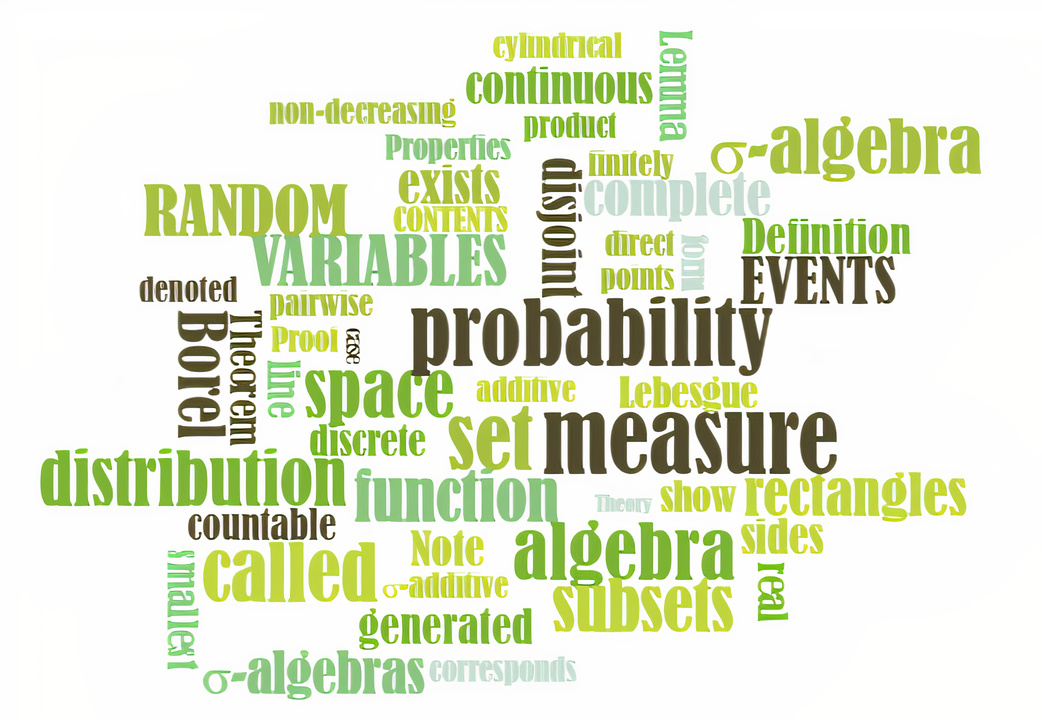
\includegraphics[scale = 1.7]{mypic.jpg}
    
    \vspace{4cm}
    \Large
    Department of Mathematics\\
    \textit{Imperial College London}\\
\end{center}}
\end{titlepage}
\newpage

We have written this set of unofficial notes to facilitate your understanding of important concepts in Probability Theory. Although most parts of the notes are based the lecture videos and in-person lectures given by Dr. Igor Krasovsky in Spring 2022, we have included additional materials drawn from various references. In particular: 

\begin{unexaminable}
\begin{itemize}
    \item Any unexaminable materials are highlighted using gray colorboxes.
\end{itemize}
\end{unexaminable}
\begin{itemize}
    \item Any unfinished/planned materials are written in \red{red}.
\end{itemize}

\textbf{Disclaimer.} These notes have not been checked by Dr. Krasovsky and should not be regarded as a replacement of the official notes and lectures for the course. In particular, all the errors are made by us, and we don't take any responsibility for their consequences; use at your own risk (and please do attend lectures -- they are fun). \\

Please email us at (insert email) with any comments or corrections.\\

Ivan Kirev and Samuel Lam \\
September 2022\\

\begin{center}
\framebox{{\sffamily Version: 0.1.4, Date: \today}}
\end{center}

\newpage 

{\pagestyle{empty}
\tableofcontents}
\newpage
\part{Measure Theory and Random Variables}
\section{Events, Probability and Random Variables}
The course aims to develop an abstract mathematical framework to describe the likelihood of certain events to happen in a random experiment. We would like to also formalise the large-sample results as developed in the probability classes you have taken in lower years, including the \textit{Law of Large Numbers} and \textit{Central Limit Theorem}.\\

To begin the story, we should understand how one can describe an experiment. You should have seen in previous probability courses that there are few key steps \footnote{as suggested in Dr. Chris Hallsworth notes on MATH50010 Probability for Statistics.} to describe an experiment:
\begin{enumerate}
    \item First describe the sets of possible outcomes $\omega$ of the experiment, which is known as \textit{sample space} $\Omega$. 
    \item Then describe the \textit{events} $A$ which we might observe as subsets of the sample space $\Omega$. We usually write the collection of such subset as $\F$. 
    \item Finally, assign a number $\p(A) \in [0,1]$ (included) to each of the subsets $A$ to quantify how likely this event might happen.
\end{enumerate}

This leads to the following fundamental problem:
\begin{itemize}
    \item What should we include in our collection of events $\F$, and
    \item How should we assign a number to those subsets in $\F$?
\end{itemize}

Let us first address the first question. For the description to make sense in reality, we should let $\F_* := \set{\varnothing, \Omega} \subseteq \F$, since we should definitely observe nothing or something in an experiment. In fact, we should probably including more subsets of $\Omega$ in $\F$ for our description to be useful. \\

A natural choice is to choose $\F = \F^* := 2^\Omega$, the \textit{power set} of $\Omega$ (which contains all subsets of $\Omega$). This is fine if $\Omega$ is countable, but will raise some issue if $\Omega$ is uncountable, e.g. $\Omega = \R$. The main concern comes from our second question: there are many properties we wish $\p$ to satisfy, e.g.  finite additivity: 

$$\forall A,B \in \F \text{ disjoint, } \p(A\cup B) = \p(A) + \p(B)$$

We can extend this naturally to countable additivity, and you should have seen that those properties would lead to contradictions! \footnote{e.g. Vitali sets, Banach-Tarski paradox. See MATH50006 Lebesgue Measure and Integration.} Therefore, we should choose $\F$ that contains $\F_*$ but is strictly smaller than $2^\Omega$.\\

Mathematicians had therefore attempted to find suitable criteria on $\F$ and $\p$ so that they would not give rise to contradictions, but still allow $\F$ to be large enough for our framework to be useful. The most successful attempt was, perhaps, made by Andrey Kolmogorov in 1933 when he devised the axioms of probability in his \textit{Grundbegriffe der Wahrscheinlichkeitsrechnung} (Foundations of the Theory of Probability), which we will cover in this chapter. His work lead to the development of the \textit{measure theory}, which forms the fundamentals of our probability theory.\\

As a final remark, the first two chapters of this course have many overlap with the courses you have done in year 1-2, so if you are familiar with the notions in these chapters, you can safely skip ahead.
\newpage

\subsection{Algebras and $\sigma$-algebras}
Let $\Omega$ be a set of points $\omega$. 
\begin{definition}[Algebra and $\sigma$-algebra] A nonempty system of subsets of $\Omega$ is called an \textbf{algebra} $\A$ if 
    \begin{itemize}
        \item $\Omega \in \A$
        \item $A,B \in \A \implies A \cup B \in A \quad (A \cap B \in \A)$
        \item $A \in \A \implies A^c \in \A$
    \end{itemize}
In addition, if all countable union $\bigcup_{n=1}^\infty A_n \in \A$ whenever $A_1, A_2, \dots \in \A$, then $\A$ is a $\sigma$-algebra. Note that then also $\bigcap_{n=1}^\infty A_n \in \F$ (consider $\Omega \backslash A_k = \hat{A}_k$).
\end{definition}

\begin{definition}[Set function and measures]
    \begin{itemize}
    \item[]
    \item A set function $\mu : \A \longrightarrow [0, \infty]$ is \textbf{finitely additive} if for any disjoint $A,B \in \A$
    \begin{equation*}
        \mu(A\cup B) = \mu(A) + \mu(B).
    \end{equation*}
    Note that then $\forall A,B \in \A$
    \begin{equation*}
        \mu(A \cup B) = \mu(A)+\mu(B) - \mu(A \cap B).
    \end{equation*}
    \item Let $\F$ be a $\sigma$-algebra. A set function $\mu : \F \rightarrow [0, \infty]$ is called $\bm{\sigma}$\textbf{-additive} if for any disjoint $A_1, A_2, ... \in \F$,
    \begin{equation*}
        \mu \bigg(\bigcup_{n=1}^\infty A_n\bigg) = \sum_{n=1}^\infty \mu(A_n). 
    \end{equation*}
    Such $\mu$ is called a \textbf{measure} on $\F$. A measure $\mu$ is called a \textbf{probability measure} if $\mu (\Omega) = 1$. Note that $\mu (\varnothing) = 0$ since $\mu(\varnothing) = \mu (\varnothing\cup \varnothing) = 2\mu (\varnothing)$. 
    \item A measure is called $\bm{\sigma}$\textbf{-finite} if there exists a representation $\Omega = \bigcup_{k=1}^\infty \Omega_k$, $\Omega_k$ - pairwise disjoint, with
    \begin{equation*}
        \mu(\Omega_k)<\infty, \quad k = 1,2,...
    \end{equation*}
\end{itemize}
\end{definition}

\begin{definition}
A \textbf{probability space} is a triple $(\Omega ,\F, \p)$, where $\Omega$ is a set called sample space, $\F$ is a $\sigma$-algebra of subsets of $\Omega$, $\p$ is a probability measure on $\F$. Any element of $\F$ is called an \textbf{event}.
\end{definition}
\begin{property}
Probability measures have the following properties:
\begin{itemize}
    \item $\p(\varnothing) = 0$;
    \item If $A,B \in \F$ then
    \begin{equation*}
        \p(A\cup B) = \p(A) + \p(B) - \p(A\cap B);
    \end{equation*}
    \item If $A,B \in \F$ and $B\subseteq A$ then
    \begin{equation*}
        \p(B) \le \p(A);
    \end{equation*}
    \item If $A_1, A_2, \dots \in \F$, then 
    \begin{equation*}
        \p \bigg( \bigcup_{n=1}^\infty A_n \bigg) \le \sum_{n=1}^\infty \p (A_n).
    \end{equation*}
\end{itemize}
\end{property}

\begin{proposition}
Let $\p$ be a finitely additive set function defined over an algebra $\A$, with $\p(\Omega) = 1$. The following four conditions are equivalent:
\begin{enumerate}[(1)]
    \item $\p$ is $\sigma$-additive (therefore it is a probability)
    \item $\p$ is continuous from below, i.e. for any sets $A_1, A_2, \dots \in \A$ such that $A_1 \subset A_2 \subset \dots$ and $\bigcup_{n=1}^\infty A_n \in \A$,
    \begin{equation*}
        \p \bigg( \bigcup_{n=1}^\infty A_n \bigg) = \lim_{n \rightarrow \infty} \p (A_n);
    \end{equation*}
    \item $\p$ is continuous from above, i.e. for any sets $B_1, B_2, \dots$ such that $B_1 \supset B_2 \supset \dots$ and $\bigcap_{n=1}^\infty B_n \in \A$,
    \begin{equation*}
        \lim_{n\rightarrow \infty} \p(B_n) = \p \bigg( \bigcap_{n=1}^\infty B_n\bigg);
    \end{equation*}
    \item $\p$ is continuous at $\varnothing$, i.e. for any sets $B_1, B_2, \dots \in \A$ such that $B_1 \supset B_2 \supset \dots$ and $\bigcap_{n=1}^\infty B_n =\varnothing$,
    \begin{equation*}
        \lim_{n \rightarrow \infty} \p(B_n) = 0.
    \end{equation*}
\end{enumerate}
\end{proposition}

\begin{proof}
$(1) \implies (2)$. Since
\begin{equation*}
    \bigcup_{n=1}^\infty A_n = A_1 \cup (A_2\backslash A_1) \cup (A_3\backslash A_2) \cup \cdots,
\end{equation*}
we have
\begin{align*}
    \p \bigg( \bigcup_{n=1}^\infty A_n \bigg) &= \p(A_1) \cup \p(A_1\backslash A_2) + \p(A_3\backslash A_2) \cup \cdots\\
    &= \p(A_1) + \p(A_2) - \p(A_1) + \p(A_3) - \p(A_2) + \cdots\\
    &= \lim_{n\rightarrow \infty} \p(A_n).
\end{align*}
$(2) \implies (3)$. Let $n \ge 1$; then
\begin{equation*}
    \p(B_n) = \p(B_1 \backslash (B_1 \backslash B_n)) = \p (B_1) - \p(B_1 \backslash B_n).
\end{equation*}
The sequence $\{ B_1 \backslash B_n \}_{n\ge1}$ of sets is non-decreasing and 
\begin{equation*}
    \bigcup_{n=1}^\infty (B_1 \backslash B_n) = B_1 \backslash \bigcap_{n=1}^\infty B_n.
\end{equation*}
Then by $(2)$
\begin{equation*}
    \lim_{n \rightarrow \infty} \p(B_1 \backslash B_n) = \p \bigg( \bigcup_{n=1}^\infty (B_1 \backslash B_n)\bigg)
\end{equation*}
and therefore
\begin{align*}
    \lim_{n \rightarrow \infty} \p(B_n) &= \p(B_1) - \lim_{n \rightarrow \infty} \p(B_1 \backslash B_n)\\
    &= \p(B_n) - \p \bigg( \bigcup_{n=1}^\infty (B_1 \backslash B_n)\bigg) = \p(B_1) - \p \bigg( (B_1 \backslash \bigcap_{n=1}^\infty B_n)\bigg)\\
    &= \p (B_1) - \p (B_1) + \p \bigg( \bigcap_{n=1}^\infty  B_n\bigg) = \p \bigg( \bigcap_{n=1}^\infty  B_n\bigg).
\end{align*}
$(3) \implies (4)$. Obvious.

$(4) \implies (1)$. Let $A_1, A_2, \dots \in \A$ be pairwise disjoint and let $ \cup_{n=1}^\infty A_n \in \A$. Then 
\begin{equation*}
    \p \bigg( \bigcup_{i=1}^\infty A_i \bigg) = \p \bigg( \bigcup_{i=1}^n A_i\bigg) + \p \bigg( \bigcup_{i=n+1}^\infty A_i \bigg),
\end{equation*}
and since $\cup_{i=n+1}^\infty A_i \downarrow \varnothing, n\rightarrow \infty$, we have 
\begin{align*}
    \sum_{i=1}^\infty \p(A_i) &= \lim_{n \rightarrow \infty} \sum_{i=1}^n \p(A_i) = \lim_{n \rightarrow \infty} \p \bigg( \bigcup_{i=1}^n A_i\bigg)\\
    &= \lim_{n \rightarrow \infty} \bigg[ \p\bigg( \bigcup_{i=1}^\infty A_i\bigg) - \p\bigg( \bigcup_{i=n+1}^\infty A_i\bigg) \bigg]\\
    &= \p \bigg( \bigcup_{i=1}^\infty A_i \bigg) - \lim_{n \rightarrow \infty}  \p \bigg( \bigcup_{i=n+1}^\infty A_i \bigg) =  \p \bigg( \bigcup_{i=1}^\infty A_i \bigg).
\end{align*}
\end{proof}



\begin{proposition}
Let $\mu$ be a finitely additive measure on an algebra $\A$ and let the sets $A_1, A_2, \dots \in \A$ be pairwise disjoint and satisfy $A = \bigcup_{i=1}^\infty A_i \in \A$. Then 
\begin{equation*}
    \sum_{i=1}^\infty \mu (A_i) \le \mu(A).
\end{equation*}
\end{proposition}

\begin{example}[$\sigma$-algebras on $\Omega$] 
Let $\Omega$ be a sample space. The following are $\sigma$-algebras:
\begin{equation*}
    \F_* = \{ \varnothing, \Omega \}; \quad \F^* = \{ A: A \in \Omega \} = 2^\Omega;
\end{equation*}
\end{example}

\begin{lemma}
For any collection $\mathcal{E}$ of subsets of $\Omega$ there exists minimal algebra $a (\mathcal{E})$ and minimal $\sigma$-algebra $\sigma(\mathcal{E})$ that contains all elements of $\mathcal{E}$ (intersection of all algebras (resp. $\sigma$-algebras) containing $\mathcal{E}$).
\end{lemma}
\begin{proof}
Intersection, countable or uncountable, of algebras (resp. $\sigma$-algebras) containing $\mathcal{E}$ is an algebra (resp. $\sigma$-algebra) containing $\mathcal{E}$.
\end{proof}
We say that $\sigma (\mathcal{E})$ is \textbf{generated} by $\mathcal{E}$.

\begin{example}[$\sigma$-algebra generated by partitions] Let $D = \{ D_1, D_2, \dots \}$ be a countable partition of $\Omega$ such that $\Omega = \bigsqcup_{j=1}^\infty D_j$. Then
\begin{equation*}
    \sigma(D) = \bigg\{ \bigcup_{j \in I}D_j : I \subset \mathbb{N} \bigg\},
\end{equation*}
To show this, we first note that the RHS is indeed a $\sigma$-algebra containing $D$. (Exercise!) Therefore we must have $\sigma(D) \subseteq$ the RHS. But since $\sigma(D)$ is closed under countable union we know that the RHS must be a subset of $\sigma(D)$. This proves the claim.
\end{example}

\subsection{Measurable Spaces}
\begin{definition}
A \textbf{measurable space} is a pair $(E, \mathcal{E})$, where $E$ is a set and $\mathcal{E}$ is a $\sigma$-algebra on $E$.
\end{definition}
\subsubsection{The measurable space $(\R, \B(\R))$}
Let $\R = (-\infty, \infty)$ be the real line and
\begin{equation*}
    (a,b] = \{ x \in \R : a < x \le b \},
\end{equation*}
for all $a,b$ with $-\infty \le a < b < \infty$. Let $\A$ be the algebra of subsets of $\R$ such that
\begin{equation*}
    A \in \A \quad \text{if} \quad  A = \bigcup_{i=1}^n (a_i, b_i] \quad n <\infty.
\end{equation*}
Let $\B(\R)$ be the smallest $\sigma$-algebra $\sigma(\A)$ containing $\A$. We observe that 
\begin{align*}
    (a,b) &= \bigcup_{n=1}^\infty \bigg(a,b-\frac{1}{n} \bigg], \quad a<b,\\
    [a,b] &= \bigcap_{n=1}^\infty \bigg(a - \frac{1}{n},b\bigg], \quad a<b,\\
    \{a\} &= \bigcap_{n=1}^\infty \bigg(a - \frac{1}{n},a\bigg].
\end{align*}
Thus the Borel algebra contains not only intervals $(a,b]$ but also the singletons $\{ a\}$ and all sets of the forms 
\begin{equation*}
    (a,b), \quad [a,b], \quad [a,b), \quad (-\infty,b), \quad (-\infty,b], \quad (a,\infty).
\end{equation*}
Let us also notice that the construction of $\B(\R)$ could have been based on any of the intervals above instead of on $(a, b]$, since all the minimal $\sigma$-algebras generated by systems of intervals of any of the forms are the same as $\B(\R)$.

\begin{exercise}
Show that $\B(\R)$ is generated by the collection of (1) open intervals of the form $(a,b)$, (2) closed intervals $[a,b]$, (3) half intervals, (4) intervals of the form $(-\infty, a]$ or $[a,\infty)$, (5) open sets and (6) closed sets with respect to the Euclidean metric.
\end{exercise}

\subsubsection{The measurable space $(\R^n, \B(\R^n))$}
Let $\R^n = \R \times \cdots \R$ be the direct product of $n$ copies of the real line, i.e. the set of ordered $n$-tuples $x = (x_1,\dots,x_n)$, where $x_k \in \R, k = 1,\dots, n$. The set
\begin{equation*}
    I = I_1 \times \cdots I_n,
\end{equation*}
where $I_k = (a_k,b_k]$, i.e. the set $\{x\in \R^n: x_k \in I_k, k=1,...,n \}$ is called a rectangle and $I_k$ is a side of the rectangle. Let $\mathcal{I}$ be the set of all rectangles $I$. The smallest $\sigma$-algebra $\sigma(\mathcal{I})$ generated by the system $\mathcal{I}$ is the Borel algebra of subsets of $\R^n$. Let us show that we can arrive at this Borel algebra by starting in a different way.
\newline

Instead of the rectangles $I = I_1 \times \cdots I_n$ let us consider the rectangles $B = B_1 \times B_2 \times \cdots \times B_n$ with Borel sides ($B_k$ is the Borel subset of the real line that appears in the $k$th place in the direct product $\R \times \cdots \times \R$).The smallest $\sigma$-algebra containing all rectangles with Borel sides is denoted by
\begin{equation*}
    \B(\R) \otimes \cdots \otimes \B(\R)
\end{equation*}
and called the direct product of the $\sigma$-algebras $\B(\R)$. Let us show that in fact
\begin{equation*}
    \B(\R^n) = \B(\R) \otimes \cdots \otimes \B(\R).
\end{equation*}
In other words, the smallest $\sigma$-algebra generated by the rectangles $I = I_1 \times \cdots \times I_n$ and the (broader) class of rectangles $B = B_1 \times \cdots \times B_n$ with Borel sides are actually the same. We need the following lemma
\begin{lemma}
Let $\mathcal{E}$ be a class of subsets of $\Omega$ and let $\B \subseteq \Omega$, and define
\begin{equation*}
    \mathcal{E} \cap B = \{ A \cap B: A \in \mathcal{E}\}.
\end{equation*}
Then 
\begin{equation*}
    \sigma(\mathcal{E}\cap B) = \sigma(\mathcal{E})\cap B.
\end{equation*}
\end{lemma}
Now we show that $\B(\R^n)$ and $\B(\R) \otimes \cdots \otimes \B(\R)$ are the same. This is obvious for $n=1$. We now show that it is true for $n=2$.
\begin{lemma}
\begin{equation*}
    \B(\R^2) = \B(\R) \otimes \B(\R)
\end{equation*}
\end{lemma}
\begin{proof}
\begin{itemize}
    \item[]
    \item $\B(\R^2) \subset \B(\R) \otimes \B(\R)$, since any open $A \subset \bigcup_{x \in A\cap \mathbb{Q}^2} R(x, \sigma(x)) \in \B(\R) \otimes \B(\R)$, $R(x, \tau)$ - open square centered at $x$ of side length $\tau(x)$.
    \item $\B(\R) \otimes \B(\R) \subset \B(\R^2)$. It is sufficient to check that $B_1 \times B_2 \in \B(\R^2)$ for any $2$ Borel sets $B_1, B_2$. Note that $B_1 \times \R \in \B(\R^2)$ since 
    \begin{equation*}
        B_1 \times \R \in \sigma(\{ \text{open subsets of } \R \}) \times \R = \sigma (\{ \text{open subsets of }\R \times \R \}),
    \end{equation*}
    Similarly, $\R \times B_2 \in \B(\R^2)$, and so 
    $B_1 \times B_2 = (B_1 \times \R) \cap (\R \times B_2) \in \B(\R^2)$.
\end{itemize}
\end{proof}
The case for any $n, n >2$ can be discussed in the same way.
\begin{remark}
Let $\B_0 (\R^n)$ be the smallest $\sigma-$ algebra generated by the open "balls"
\begin{equation*}
    S_\rho (x^0) = \{ x \in \R^n: \rho_n (x, x^0) < \rho \}, \quad x^0 \in \R^n, \rho > 0,
\end{equation*}
in the metric 
\begin{equation*}
    \rho_n (x,x^0) = \sum_{k=1}^n 2^{-k} \rho_1(x_k, x_k^0),
\end{equation*}
where $x = (x_1, \dots, x_n),$ $x^0 = (x_1^0, \dots, x_n^0).$ Then $\B_0(\R^n) = \B(\R^n)$ (exercise).
\end{remark}

\subsubsection{The measurable space $(\R^\infty, \B(\R^\infty))$}
This space plays a significant role in probability theory, since it is used as the basis for constructing probabilistic models of experiments with infinitely many steps. Let $\R^\infty = \{  x = (x_1, x_2, \dots ), x_k \in \R \}$.
\begin{definition}
A set $C \subset \R^\infty$ is called \textbf{cylindrical} if it is of the form $C = \{ x \in \R^\infty :(x_1, x_2, ..., x_n) \in \tilde{C}_n \}$ for some $n \ge 1$ and $\tilde{C}_n \in \B(\R^n)$.
\end{definition}
Cylindrical sets form an algebra (check!) which generates a $\sigma$-algebra called cylindrical $\sigma$-algebra, denoted $\B(\R^\infty)$. One can verify that
\begin{equation*}
    \B(\R^\infty) = \sigma(\{ A_1 \times A_2 \times \cdots \subset \R^\infty, A_k \in \B(\R) \}).
\end{equation*}
\begin{example}
For all $c \in \R$, let $A = \{ x \in \R^\infty : \limsup_n x_n = \inf_n \sup_{k>n} x_k > c \}$. We have $A \in \B(\R^\infty)$: indeed
\begin{equation*}
    A = \bigcap_{n=1}^\infty \bigcup_{k = n+1}^\infty \{ x \in \R^\infty: x_k > c \} = (x_k > c \quad i.o.).
\end{equation*}
For all $c$ let 
\begin{equation*}
    B = \{ x \in \R^\infty: \liminf_n x_n = \sup_n \inf_{k>n} x_k > c \}.
\end{equation*}
We have $B \in \B(\R^\infty)$: indeed
\begin{equation*}
    B = \bigcap_{n=1}^\infty \bigcup_{k = n+1}^\infty \{ x \in \R^\infty: x_k > c \} = (x_k > c \quad ev.).
\end{equation*}
For all $c$, $D = \{ x\in \R^\infty : \lim_{n \rightarrow \infty} x_n = c \} \in \B(\R^\infty)$ (exercise).
\end{example}
Recall: non-decreasing function $g(x)$ on $\R$ is continuous up to possibly countably many discontinuities of first kind: $f(x+0),$ $f(x-0)$ both exist, but $f(x+0)-f(x-0) = h_x>0$. Moreover, the derivative $g'(x)$ exists Lebesgue a.e.

\begin{unexaminable}
\begin{remark} \label{rmk:PolishSpace} We can generalise the notion of Borel $\sigma$-algebra to other sample spaces. Assume $\Omega$ is \textbf{Polish}, i.e. a metric space which is
\begin{itemize}
    \item \textbf{complete}: all Cauchy sequences $(\omega_k)_{k\geq 1}$ has a limit $\omega \in \Omega$, and 
    \item \textbf{separable}: there exists a countable subset $E :=  \set{\omega_k}_{k\geq 1}$ which is dense in $\Omega$, or $\bar{E} = \Omega$
\end{itemize}
then we can define the Borel $\sigma$-algebra of $\Omega$ $\B(\Omega)$ as the smallest $\sigma$-algebra containing all open subsets of $\Omega$. We can then talk about the Borel $\sigma$-algbera of e.g. the space of all continuous function of $[0,1]$, $\Omega = C^0([0,1])$, equipped with the supremum metric $d(f,g) = \sup_{[0,1]} |f-g|$.
\end{remark}

In fact, we will look at probability measures on Polish space quite often in Chapter 5 when we talk about weak convergence. If you are not comfortable with dealing with general Polish spaces, just treat them as $(\R,\B(\R))$ for the first reading. However, we will still try to incorporate discussions about measures on a general Polish space as they laid the foundation of stochastic processes. A few applications include:
\begin{itemize}
\item Continuous-time random walk (e.g. Brownian motion) - this could obviously be viewed as an indexed family of real-valued random variable $B_t(\omega), t \geq 0$, but one can also treat it as \textbf{one single} random variable $B(\omega) \in C^0[0,1].$
\item Empirical processes (i.e. "sample" cumulative distribution function) - this is usually treated as a random variable with an output of a distribution function (as defined below).
\end{itemize}

Therefore, we would encourage you to understand important results related to measures on a general Polish space before delving deep into the theory of stochastic processes.
\end{unexaminable}

\subsection{Probability Measures on Measurable Spaces}
\subsubsection{Probability Distributions}
We begin by the following observation.
\begin{exercise}
Let $(\R, \B(\R), \p)$ be a probability space and denote $F(x) := \p(-\infty, x]\quad x \in \R$. Show that:
\begin{itemize}
    \item $F(x)$ is non-decreasing,
    \item $\lim_{x\rightarrow -\infty} F(x) = 0$, $\lim_{x \rightarrow \infty} F(x) = 1$, and
    \item $F(x)$ is continuous on the right for all $x \in \R$.
\end{itemize}
\end{exercise}


\begin{definition}
Every function $F: \R \longrightarrow [0,1]$ satisfying the above three conditions is called a \textbf{distribution function} (on  the real line $\R$).
\end{definition}

Thus to every probability measure $\p$ on $(\R, \B(\R))$, there corresponds a distribution function. In fact, the opposite is also true and there exists one to one correspondence between distribution functions and probability measures:
\begin{theorem}
Let $F = F(x)$ be a distribution function on $\R$. Then there exists a unique probability measure $\p$ on $(\R, \B(\R))$ such that $$\p(a, b] = F(b) - F(a),$$
for all $a,b, -\infty \le a < b < \infty.$
\end{theorem}

This relies on the following fundamental result in measure theory.
\begin{theorem}[Caratheodory Theorem]
Let $\mu_0$ be a $\sigma$-additive (pre-)measure on $(\Omega, \A)$, where $\A$ is an algebra of subsets of $\Omega$. Then there exists a unique measure $\mu$ on $(\Omega, \sigma(\A))$, such that 
\begin{equation*}
    \mu (A) = \mu_0(A) \quad \forall A \in \A.
\end{equation*}
\end{theorem}

We make a few remarks on this theorem, the first one being the completeness of measure. Recall the following:
\begin{definition}[Complete measure]
A measure $\mu$ on a $\sigma$-algebra $\Sigma$ on $\Omega$ is called complete if any subset of a set of measure zero (null sets) is measurable, i.e. belongs to $\Sigma$.
\end{definition}

We introduce this notion of completeness to avoid any caveats in proving results relating to measures. Note that $(\R, \B(\R), \p)$ with $\p$ constructed from the Caratheodory theory above is not complete ($\exists$ subsets of a Borel set which are not Borel). Fortunately, one can enlarge the $\sigma$-algebra so that it includes all null sets: if a measure $\mu$ on $\Sigma$ is not complete, it can be completed by extending $\Sigma$ to 
\begin{equation*}
    \overline{\Sigma} = \sigma(\Sigma \cup \{ B \in \Omega : B \subset A \in \Sigma, \mu(A) = 0 \}),
\end{equation*}

and the definition of $\mu$ so that $\mu(B) = 0$ for any $B$ being a subset of a null set. This is a fundamental result that should be checked by yourself. The completion of the measure obtained from the Caratheodory theorem is called the \textit{Lebesgue-Stiltjes measure}. In particular, the distribution function $F(x) = x$ corresponds to the Lebesgue measure on $\R$.\\

The second remark concerns measure determining sets. Given two measures $\mu, \nu$ defined on a common measurable space $(\Omega,\F)$. How many sets do we need to check for us to show that $\mu = \nu$? The Caratheodory Theorem suggests that one may look at the algebra $\A$ such that $\F = \sigma(\A)$, but the following theorem suggests that one might look at a far smaller collection of subsets of $\Omega$: 

\begin{theorem}[Measure Determining Set] \label{thm:measure_determining}
Consider a measurable space $(\Omega,\F)$ with measures $\mu, \nu$, and let $\cC$ be a $\pi$-system containing $\Omega$ (in the sense that $A, B \in \cC$ implies $A \cap B \in \cC$). If $\mu(B) = \nu(B)$ for all $B \in \cC$, then $\mu = \nu$.
\end{theorem}

The key idea is to note that the collection $\set{B \in \F \,|\, \mu(B) = \nu(B)}$ is a Dynkin $\lambda$-system (which is non-empty, closed under complement and countable disjoint union). Since $\cC$ above is a sub-collection of this collection, we know from $\pi$-$\lambda$ theorem that $\sigma(\cC)$ is contained in this collection. Therefore if one can show that $\sigma(\cC) = \F$ then we have proven $\mu = \nu$. We will not go through the technical details here.

\begin{example} \label{eg:measures_determined_by_open_closed_sets}
As an application, any probability measure on $(\R,\B(\R))$ is determined by open, closed or half-open intervals. In other words, e.g. if $\mu, \nu$ are probability measures on $(\R,\B(\R))$ such that $\mu(O) = \nu(O)$ for all $O$ being open intervals, then $\mu = \nu$.
\end{example}

\begin{unexaminable}
\begin{example}
We can generalise this to the following: for probability measure defined on a Polish space $(X,\B(X))$, it is determined by open or closed sets in the above sense.
\end{example}
\end{unexaminable}

\subsubsection{Continuity of Measures on $(\R, \B(\R))$}

\textbf{Discrete/Atomic measures} are measures $\p$ for which the corresponding distributions $F = F(x)$ are piecewise constant, changing their values at the points $x_1, x_2, \dots$ ($\Delta F(x_i) >0$, where $\Delta F(x) = F(x) - F(x^-))$. 
\begin{center}
    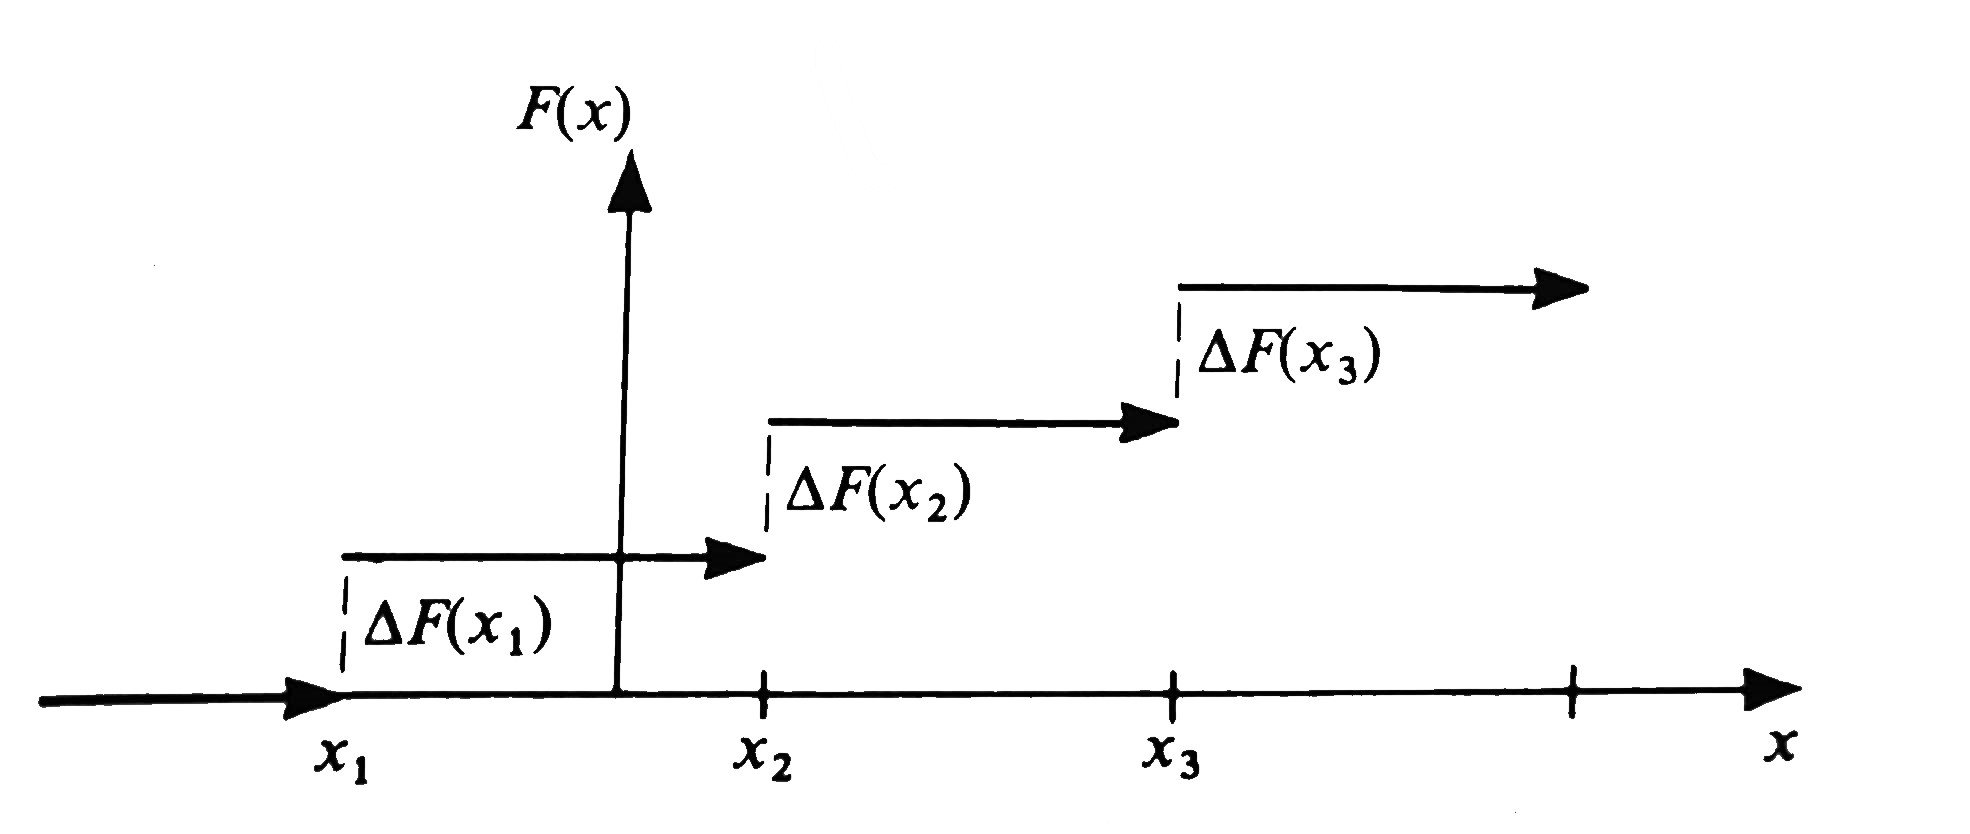
\includegraphics[scale = 0.2]{1.jpg}
    \captionof{figure}{CDF of a (purely) atomic measure.}
\end{center}

In this case the measure is concentrated at the points $x_1, x_2, \dots$, known as \textbf{atoms}:
\begin{equation*}
    \p(\{ x_k \}) = \Delta F(x_k)>0, \quad \sum_k \p(\{x_k \}) = 1
\end{equation*}
The set of numbers $(p_1, p_2, \dots)$, where $p_k = \p\{x_k\}$, is called a \textbf{discrete probability distribution} and the corresponding distribution function 
\begin{equation*}
    F(x) = F_{\mathsf{disc}}(x) = \sum_{x_k \le x}p_k, \quad \quad \dots, p_1, p_2, \dots >0
\end{equation*}
is called \textbf{discrete}.
\begin{example}
\begin{itemize}
    \item[]
    \item Discrete Uniform distribution: $p_k = \frac{1}{N}, \quad k = 1,2,\dots, N, \quad N$ - fixed.
    \item Bernoulli $\sB(1,p)$: $p_1 = p, p_2 = 1-p,\quad 0 \le p \le 1.$
    \item Binomial $\sB(n,p)$: $p_k = \binom{n}{k} p^k (1-p)^k,\quad k = 0,1,\dots,n \quad 0 \le p \le 1.$
    \item Poisson $\Po(\lambda)$: $p_k = e^{-\lambda}\frac{\lambda^k}{k!}, \quad \lambda>0,\quad k = 0,1,\dots$
\end{itemize}
\end{example}
\textbf{Absolutely continuous measures}. We begin by noting the following observation:
\begin{proposition}
Let $f$ be an integrable function \footnote{see Chapter 2} $f(x) \ge 0$ such that
\begin{equation*}
    F(x) = F_{\mathsf{ac}}(x) = \int_{-\infty}^x f(t) \, \d t \quad \text{w.r.t Lebesgue measure}
\end{equation*}
Then the set function $\p_{ac}(A) = \int_{A} f(t)\d t \quad A \in \F$ is a measure. In particular, we say that $f$ is a density of $\p_{\mathsf{ac}}$.
\end{proposition}
\begin{proof}
First assign $\p_{ac}((a,b]) = \int_a^bf(t)\d t$, then use Caratheodory theorem to extend to $\sigma$-algebra.
\end{proof}
Measures of such kind is \textbf{absolutely continuous} (with respect to the Lebesgue measure $\mu$) in the following sense: if $\mu(A) = 0$ then $\p_{\mathsf{ac}}(A) = 0$. Indeed,

\begin{theorem}[Radon-Nikodym] If $\p$ is a measure such that $\mu(A) = 0\implies \p(A) = 0$, then $\p$ has a density.
\end{theorem}

Note that there is a connection between absolute continuity of measures and absolute continuity of functions: if $\p$ is an absolutely continuous measure then $F_{ac}(x)$ is an absolutely continuous function, and that $F'_{ac}(x) = f(x)$ almost everywhere.\\

Finally, the notion of absolute continuity can be generalised. This is useful in constructing conditional expectations: see Chapter 8.

\begin{example}
\begin{itemize}
    \item[]
    \item Uniform distribution on $[a,b]$: $f(x) = 1/(b-a), \quad a\le x \le b, \quad f(x) = 0$ otherwise.
    \item Normal or Gaussian: $f(x) = (2\pi \sigma^2)^{-1/2}\exp{\frac{-(x-m)^2}{2\sigma^2}}, \quad x \in \R, \quad \sigma >0.$
    \item Gamma: $f(x) = \frac{x^{\alpha - 1}e^{-x/\beta}}{\Gamma(\alpha)\beta^\alpha}, \quad x \ge 0 \quad \alpha, \beta >0$
\end{itemize}
\end{example}
Recall that a measure $\nu$ is said to be \textbf{concentrated} on a measurable set $A$ if $\nu(E) = 0$ for any $E \subset \R\backslash A$.\\

\textbf{Singular continuous}. These are measures whose distribution functions are continuous but have all their points of increases on sets of zero Lebesgue measure. We have that $F(x) = F_{\mathsf{sc}}(x)$ is continuous at any $x$ and $\p_{\mathsf{sc}}$ is concentrated on a set of Lebesgue measure zero. In particular this distribution has no atoms. For $x$ in this set, $F'_{\mathsf{sc}}(x) \ne 0$ or does not exist. Thus $F'_{sc}(x) = 0$ a.e. Note that, by continuity, $\p_{\mathsf{sc}}\{x\} = 0$ for each point $x\in \R$.
\begin{example}[Cantor's Devil staircase]
We consider the interval $[0,1]$ and construct $F(x)$ by the following procedure originated by Cantor. 
\begin{center}
    \begin{tikzpicture}
    \begin{axis}[
    axis lines=left,
    xlabel = $x$, ylabel = $F(x)$,
    xmax = 1.1, xtick = {0, 1/3, 2/3, 1}, 
    ymax = 1.1, ytick = {0, 1/2, 1},
    xticklabels={$0$, $1/3$, $2/3$, $1$},
    yticklabels={$0$, $1/2$, $1$}, 
    width=0.6\textwidth, height=0.4\textwidth]
    \addplot[domain=0:1/3] {3*x/2};
    \addplot[domain=1/3:2/3] {1/2};
    \addplot[domain=2/3:1] {3*(x-1)/2 + 1};
    \end{axis}
\end{tikzpicture}
    \captionof{figure}{First step of constructing the devil staircase.}
\end{center}
We divide $[0,1]$ into thirds and put 
\begin{equation*}
    F_2(x) =
    \begin{cases}
     1/2, & x\in (\frac13, \frac23)\\
     1/4, & x \in (\frac19, \frac29)\\
     3/4, & x \in (\frac79, \frac89)\\
     0, & x = 0\\
     1, & x=1
    \end{cases}
\end{equation*}
defining it in the intermediate intervals by linear interpolation. Then we divide each of the intervals $[0,1/3]$ and $[2/3, 1]$ into three parts and define the function shown below with its values at other points determined by linear interpolation.
\begin{center}
    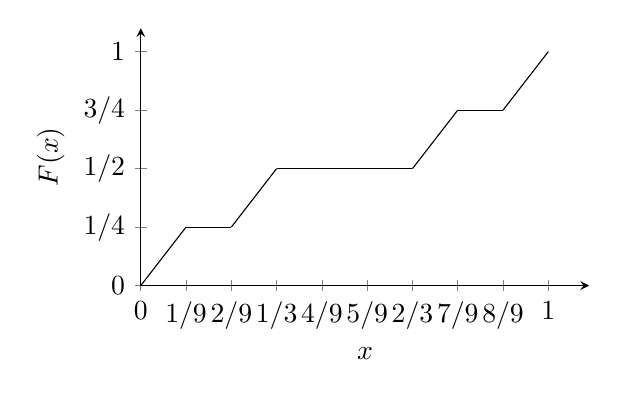
\begin{tikzpicture}
    \begin{axis}[
    axis lines=left,
    xlabel = $x$, ylabel = $F(x)$,
    xmax = 1.1, xtick = {0, 1/9, 2/9, 3/9, 4/9, 5/9, 6/9, 7/9, 8/9, 1}, 
    ymax = 1.1, ytick = {0, 1/4, 1/2, 3/4, 1},
    xticklabels={$0$, $1/9$, $2/9$, $1/3$, $4/9$, $5/9$, $2/3$, $7/9$, $8/9$, $1$},
    yticklabels={$0$, $1/4$, $1/2$, $3/4$, $1$}, 
    width=0.6\textwidth, height=0.4\textwidth]
    \addplot[domain=0:1/9] {9*x/4};
    \addplot[domain=1/9:2/9] {1/4};
    \addplot[domain=2/9:1/3] {9*(x-1/3)/4 + 1/2};
    \addplot[domain=1/3:2/3] {1/2};
    \addplot[domain=2/3:7/9] {9*(x-7/9)/4 + 3/4};
    \addplot[domain=7/9:8/9] {3/4};
    \addplot[domain=8/9:1] {9*(x-1)/4 + 1};
    \end{axis}
\end{tikzpicture}
    \captionof{figure}{Second step of constructing the devil staircase.}
\end{center}
Continuing with this process, we construct a sequence of functions $F_n(x)$, $n= 1,2,\dots$ which converges to a non-decreasing continuous function $F(x)$ (the Cantor function), whose points of increase form a set of Lebesgue measure zero. In fact, it is clear from the construction of $F(x)$ that the total length of the intervals $(\frac13, \frac23), (\frac19, \frac29), (\frac79, \frac89), \dots$ on which the function is constant is
\begin{equation*}
    \frac13 + \frac29 + \frac{4}{27} + \cdots = 1.
\end{equation*}
Let $N$ be the set of points of increase of the Cantor function $F(x)$. It follows from the sum above that $\Leb(N) = 0$. At the same time, if $\mu$ is the measure corresponding to the Cantor function $F(x)$, we have $\mu(N) = 1$. (We then say that the measure is singular with respect to the Lebesgue measure $\Leb$.)
\end{example}
\begin{theorem}[Hahn decomposition]
Any probability distribution has a representation:
\begin{equation*}
    F(x) = a_1F_{\mathsf{disc}}(x) + a_2 F_{\mathsf{ac}}(x) + a_3F_{\mathsf{sc}}(x), \quad a_1+a_2+a_3 =1.
\end{equation*}
\end{theorem}

\subsubsection{Probability Measures on $(\R^n, \B(\R^n))$}

Distribution functions on $(\R^n, \B(\R^n))$ are defined similarly, e.g.
\begin{equation*}
    F(x,y) = \p((-\infty, x] \times (-\infty, y]), \quad n=2
\end{equation*}
The product measure on $(\Omega_1 \times \Omega_2, \F_1 \otimes \F_2)$ is defined as follows. First set $$\p_0(A_1 \times A_2) = \p_1(A_1)\p_2(A_2)$$ for $A_1 \in \F_1, A_2 \in \F_2$. (Probability spaces $(\Omega_1, \F_1, \p_1)$, $(\Omega_2, \F_2, \p_2))$ Then extend $\p_0$ to the algebra generated by $A_1 \times A_2,$ show that $\p_0$ is a $\sigma$-additive measure on this algebra, and apply Caratheodory theorem to obtain the extension. This extension is called the product measure, denoted $\p_1 \otimes \p_2$.\\

\subsubsection{Probability Measures on $(\R^\infty, \B(\R^\infty))$}
For the spaces $\R^n$, $n \ge 1$, the probability measures were constructed in the following way: first for elementary sets (rectangles $(a, b]$), then, in a natural way, for sets $A = \sum (a_i, b_i]$, and finally, by using Caratheodory’s theorem, for sets in $\B(\R^n)$.\\

A similar procedure of constructing probability measures also works for the space $(\R^\infty, \B(\R^\infty))$. Let
\begin{equation*}
    \mathcal{I}_n(B) = \{ x \in \R^\infty : (x_1, \dots, x_n) \in B\}, \quad B \in \B(\R^n),
\end{equation*}
denote a cylinder set in $\R^\infty$ with base $B \in \B(\R^n)$. As we will see now, it is natural to take the cylinder sets for the elementary sets in $R^\infty$ whose probabilities enable us to determine the probability measure on the sets of $\B(\R^\infty)$.\\

We now define the notion of consistent sequence of measures:

\begin{definition}[Consistent Sequence] \label{def:consistent_sequence}
The sequence $\p_n$ of probability measures on $(\R^n, \B(\R^n))$ is said to be \textbf{consistent} if for all $n = 1,2, \dots$ and $B \in \B(\R^n)$,
\begin{equation*}
    \p_{n+1}(B \times \R) = \p_n (B).
\end{equation*}
\end{definition}

The following theorem states that we can always construct a probability measure on $(\R^\infty, \B(\R^\infty))$ based on a consistent sequence of measures:
\begin{theorem}[Kolmogorov Extension Theorem] \label{thm:kolmogorov_extension}
For any consistent sequence $\p_n$ on $(\R^n, \B(\R^n))$, there exists a unique probability measure $\p$ on $(\R^\infty, \B(\R^\infty))$ such that 
\begin{equation*}
    \p(\mathcal{I}_n(B)) = \p_n(B), \quad B \in \B(\R^n),
\end{equation*}
for $n = 1,2,\dots$.
\end{theorem}

\begin{unexaminable}
\begin{proof}
Let $B^n \in \B(\R^n)$ and let $\mathcal{I}_n(B^n)$ be the cylinder with base $B^n$. We assign the measure $\p(\mathcal{I}_n(B^n))$ to this cylinder by taking 
\begin{equation*}
    \p(\mathcal{I}_n(B^n)) = \p_n(B^n).
\end{equation*}
Let us show that, in virtue of the consistency condition, this definition is consistent, i.e., the value of $\p(\mathcal{I}_n(B^n))$ is independent of the representation of the set $\mathcal{I}_n(B^n)$. In fact, let the same cylinder be represented in two ways:
\begin{equation*}
    \mathcal{I}_n(B^n) = \mathcal{I}_{n+k}(B^{n+k}).
\end{equation*}
It follows that, if $(x_1, \dots, x_{n+k}) \in \R^{n+k}$, we have 
\begin{equation*}
    (x_1, \dots, x_n) \in B^n \iff (x_1, \dots, x_{n+k}) \in B^{n+k},
\end{equation*}
and therefore, 
\begin{align*}
    \p_n(B^n) &= \p_{n+1}((x_1, \dots, x_{n+1}): (x_1, \dots, x_{n}) \in B^n)\\
    &= \dots = \p_{n+k}((x_1, \dots, x_{n+k}): (x_1, \dots, x_{n}) \in B^n)\\
    &= \p_{n+k}(B^{n+k}).
\end{align*}
Let $\mathcal{A}(\R^{\infty})$ denote the collection of all cylinder sets $\hat{B}^n = \mathcal{I}_n(B^n), B^n \in \B(\R^n), n=1,2,\dots$. It is easy to see that $\mathcal{A}(\R^\infty)$ is an algebra.\\

Now let $\hat{B}_1, \dots, \hat{B}_k$ be disjoint sets in $\mathcal{A}(\R^\infty)$. We may suppose without loss of generality that $\hat{B}_i = \mathcal{I}_n(B_i^n), i=1, \dots, k$, for some $n$, where $B_1^n, \dots, B_k^n$ are disjoint sets in $\B(\R^n)$. Then
\begin{equation*}
    \p \bigg( \sum_{i=1}^k \hat{B}_i \bigg) = \p \bigg( \sum_{i=1}^k \mathcal{I}_n(B_i^n) \bigg) = \p_n \bigg( \sum_{i=1}^k B_i^n\bigg) = \sum_{i=1}^n \p_n(B_i^n) = \sum_{i=1}^n \p(\hat{B}_i),
\end{equation*}
i.e. the set function $\p$ is finitely additive on the algebra $\mathcal{A}(\R^\infty)$.

Let us show that $\p$ is continuous at zero (and therefore $\sigma$-additive on $\mathcal{A}(\R^\infty)$), i.e., if a sequence of sets $\hat{B}_n \downarrow \emptyset$, $n \to \infty$, then $\p(\hat{B}_n) \to 0,$ $n\to \infty$. Suppose the contrary, i.e., let $\lim \p(\hat{B}_n) = \delta > 0$ (the limit exists due to monotonicity). We may suppose without loss of generality that $\{\hat{B}_n\}$ has the form 
\begin{equation*}
    \hat{B}_n = \{ x : (x_1, \dots , x_n) \in B_n \}, \quad B_n \in \B(\R^n).
\end{equation*}
We use the following property of probability measures $\p_n$ on $(\R^n, \B(\R^n))$: if $B_n \in \B(\R^n)$, for a given $\delta > 0$ we can find a compact set $A_n \in \B(\R^n)$ such that $A_n \subset B_n$ and
\begin{equation*}
    \p_n(B_n \backslash A_n) \le \delta/ 2^{n+1}.
\end{equation*}
Therefore, if 
\begin{equation*}
    \hat{A}_n = \{ x:(x_1, \dots, x_n) \in A_n\},
\end{equation*}
we have
\begin{equation*}
    \p(\hat{B}_n \backslash \hat{A}_n) = \p(B_n \backslash A_n) \le \delta/ 2^{n+1}.
\end{equation*}
Form the set $\hat{C}_n = \bigcap_{k=1}^n \hat{A}_k$ and let $C_n$ be such that 
\begin{equation*}
    \hat{C}_n = \{ x: (x_1, \dots, x_n) \in C_n \}.
\end{equation*}
Then, since the sets $\hat{B}_n$ decrease, we obtain 
\begin{equation*}
    \p(\hat{B}_n \backslash \hat{C}_n) \le \sum_{k=1}^n \p(\hat{B}_k \backslash \hat{A}_k) \le \delta/2.
\end{equation*}
But by assumption, $\lim_n \p(\hat{B}_n) = \delta > 0$, and therefore $\lim_n \p(\hat{C}_n) \ge \delta/2 > 0$. Let us show that this contradicts the condition $\hat{C}_n \downarrow \emptyset$.\\

Let us choose a point $\hat{x}^{(n)} = (x_1^{(n)}, x_2^{(n)},\dots)$ in $\hat{C}_n$. Then $(x_1^{(n)}, \dots, x_n^{(n)}) \in C_n$ for $n\ge 1$.

Let $(n_1)$ be a subsequence of $(n)$ such that $x_1^{(n_1)} \to x_1^{0}$, where $x_1^0$ is a point in $C_1$. (Such a sequence exists since $x_1^{(n_1)} \in C_1$ and $C_1$ is compact.) Then select a subsequence $(n_2)$ of $(n_1)$ such that $(x_1^{(n_2)}, x_2^{(n_2)}) \to (x_1^0, x_2^0) \in C_2$. Similarly let $(x_1^{(n_k)}, \dots, x_k^{(n_k)}) \to (x_1^0,\dots,  x_k^0) \in C_k$. Finally, from the diagonal sequence $(m_k)$, where $m_k$ is the $k$th term of $(n_k)$. Then $x_i^{(m_k)} \to x_i^0$ as $m_k \to \infty$ for $i=1,2, \dots$, and $(x_1^0, x_2^0, \dots)\in \hat{C}_n$ for $n = 1,2,\dots$, which evidently contradicts the assumption that $\hat{C}_n \downarrow \emptyset$, $n \to \infty$. Thus the set function $\p$ is $\sigma$-additive on the algebra $\mathcal{A}(\R^\infty)$ and hence, by the Caratheodory's theorem, it can be extended to a (probability) measure on $(\R^\infty, \B(\R^\infty))$. This completes the proof of the theorem.
\end{proof}
\end{unexaminable}
%\subsubsection{Banach-Tarski Paradox}

%\begin{theorem}[Banach-Tarski paradox]
%A unit ball in $\R^3$ can be partitioned into $5$ parts that can be reassembled (shifts + rotations) to form $2$ non-intersecting unit balls.
%\end{theorem}

\subsection{Random Variables}
Let $(\Omega, \F, \p)$ be a probability space.

\begin{definition}[Random variable]
A real function $\xi: \Omega \rightarrow \R$ is an \textbf{$\F$-measurable function}, or a \textbf{random variable} if
\begin{equation*}
    \{ \omega: \xi(\omega) \in B \} \in \F
\end{equation*}
for every $B \in \B(\R)$; or equivalently, if the inverse image
\begin{equation*}
    \xi^{-1}(B) \equiv \{ \omega: \xi(\omega) \in B \}
\end{equation*}
is a measurable set in $\Omega$. When $(\Omega, \F) = (\R^n, \B(R^n)),$ the $\B(R^n)$-measurable functions are called \textbf{Borel functions}.
\end{definition}

Random variables are used to \textit{summarise} certain abstract outcomes $\omega$ with a real number / vector etc. A good example is the following:

\begin{example}[Sum of two dices] Consider the experiment of throwing two independent fair six-faced dices. This can be represented by the probability space $(\Omega_1, \F_1, \p_1) \otimes (\Omega_2, \F_2, \p_2)$, where for $i=1,2$, $\Omega_i = \set{1,2,3,4,5,6}$ is the outcome from dice $i$, $\F_i = 2^{\Omega_i}$ and $\p_i(\set{j}) \equiv 1/6$ for all $j \in \set{1,2,3,4,5,6}$. We can then consider the function $X: \Omega_1 \times \Omega_2 \to \R$ by $$X(\omega_1, \omega_2) = \omega_1 + \omega_2$$
which summarises the outcome of two dices by their sum. One can easily check that $X$ is a measurable function by looking at the possible pre-images of $X$, and we will leave it as an exercise.
\end{example}

\begin{exercise}
In the example above,
\begin{itemize}
    \item What are the possible outcomes of $X$?
    \item What are the possible pre-images of $X$? Notice they are subsets of $\F_1 \otimes \F_2 = 2^{\Omega_1 \times \Omega_2}$.
\end{itemize}
\end{exercise}

\begin{remark}
Let $\xi$ be a random variable. If we consider sets from $\F$ of the form $\{ \omega: \xi(\omega) \in B \}, B \in \B(\R)$, it is easily verified that they form a $\sigma$-algebra, called the \textbf{$\sigma$-algebra generated by $\xi$}, denoted by $\F_\xi$ and $\F_\xi \subset \F$. 
\end{remark}

\subsubsection{Operations of Random Variables}

\begin{lemma}
Let $\mathcal{D}$ be a collection of subsets on $\R$ such that $\sigma(\mathcal{D}) = \B(\R)$. A necessary and sufficient condition that a function $\xi = \xi(\omega)$ is a random variable is that
\begin{equation*}
    \xi^{-1}(D) = \{ \omega: \xi(\omega) \in D \} \in \F
\end{equation*}
for all $D \in \mathcal{D}$.
\end{lemma}
\begin{corollary}
A necessary and sufficient condition for $\xi = \xi(\omega)$ to be a random variable is that
\begin{equation*}
    \{ \omega: \xi(\omega) < x \} \in \F
\end{equation*}
for every $x \in \R$, or that
\begin{equation*}
    \{ \omega: \xi(\omega) \le x \} \in \F
\end{equation*}
for every $x \in \R$.
\end{corollary}
\begin{lemma}
Let $\varphi = \varphi(x)$ be a Borel function and $\xi = \xi(\omega)$ a random variable. Then the composition $\eta = \varphi \circ \xi$, i.e. the function $\eta(\omega) = \varphi(\xi(\omega))$, is also a random variable (and, in fact, $\F_\xi$- measurable).
\end{lemma}
\begin{proof}
The proof follows from the equations:
\begin{equation*}
    \{w:\eta(\omega) \in B \} = \{w:\varphi(\xi(\omega)) \in B \} = \{w:\xi(\omega) \in \varphi^{-1}(B)  \} \in \F
\end{equation*}
for $B \in \B(\R)$, since $\varphi^{-1}(B) \in \B(\R)$.
\end{proof}

\begin{example}
\begin{itemize}
    \item[]
    \item If $\xi$ is a random variable and $f: \R \rightarrow \R$ is a continuous function then $f(\xi)$ is a random variable.
    \item If $\xi$ is a random variable, then so are $\xi^n, \xi^+ = \max(\xi,0), \xi^-=-\min(\xi,0),$ and $|\xi| = \xi^+ + \xi^-$
\end{itemize}
\end{example}

\begin{lemma}
If $\xi,\eta$ are random variables, then 
\begin{equation*}
    \xi + \eta, \xi - \eta, \xi \eta, \xi/ \eta, \max{(\xi,\eta)}, \min{(\xi,\eta)}
\end{equation*}
are random variables (assuming that they are defined, i.e. no forms like $\infty - \infty, \infty/\infty,  a/0$ occur).
\end{lemma}

\begin{lemma}
If $f_n,$ $n = 1,2, \dots$ are random variables and if $\forall \omega$  $$s(\omega) = \sup_n f_n(\omega)$$
exits, then $s(\omega)$ is a random variable. Similarly, we can replace $\sup_n$ with $\inf_n$ or $\lim_n$.
\end{lemma}

\begin{definition}
A random variable $\xi$ is called \textbf{simple} if 
\begin{equation*}
    \xi(\omega) = \sum_{j=1}^n x_j \chi_{D_j}(\omega)
\end{equation*}
for some $n \ge 1$ and a partition $D_1, D_2, \dots, D_n$ of $\Omega$, where
\begin{equation*}
    \chi_D(\omega) = 
    \begin{cases}
     1, & \omega \in D\\
     0, & \text{otherwise}
    \end{cases}
\end{equation*}
\end{definition}
\begin{lemma}
\begin{itemize}
    \item[]
    \item For every random variable $\xi = \xi(\omega)$ there is a sequence of simple random variables $\xi_1, \xi_2, \dots$, such that $|\xi_n| \le |\xi|$ and $\xi_n(\omega) \rightarrow \xi(\omega), n \rightarrow \infty$, for all $\omega \in \Omega$.
    \item For any random variable $\xi(\omega) \ge 0$ there exists a pointwise non-decreasing sequence of simple random variables $\xi_1(\omega) \le \xi_2(\omega) \le \dots \le \xi(\omega)$ such that 
    \begin{equation*}
        \lim_{n \rightarrow \infty} \xi_n(\omega) = \xi(\omega) \quad \forall \omega \in \Omega \quad (\text{in short }\xi_n\nearrow\xi)
    \end{equation*}
\end{itemize}
\end{lemma}
\begin{proof}
We begin by proving the second statement. For $n=1,2,\dots$, put 
\begin{equation*}
    \xi_n(\omega) = \sum_{j=0}^{n2^n-1} \frac{j}{2^n}\chi_{ \big\{\omega: \frac{j}{2^n} \le \xi(\omega)< \frac{j+1}{2^n}  \big\}} + n \chi_{\{\omega: \xi(\omega)\ge n \}}
\end{equation*}
It is easy to verify that the sequence $\xi_n(\omega)$ so constructed is such that $\xi_n\nearrow\xi$ for all $\omega \in \Omega$. The first statement follows from this if we merely observe that $\xi$ can be represented in the form $\xi = \xi^+ - \xi^-,$ where $\xi^+ = \max(\xi,0)$ and $\xi^-= \max(-\xi,0).$
\end{proof}

The below figures represent how one can build simple function approximation to the function $f(x) = x^2$ for all $x \in \R$. For simplicity, only the first two steps are shown.
\begin{figure}[h]
    \centering
    \begin{subfigure}[h]{0.45\textwidth}
        \centering
        \begin{tikzpicture}
            \begin{axis}[
            axis lines=center,
            xlabel = $x$,
            xmin = -1.8, xmax = 1.8,
            ymin = -0.5, ymax = 2.5, 
            height = 0.24\textheight, 
            width=\textwidth
            ]
            \addplot[domain=-1.8:1.8, color=blue] {x^2};
            \addplot[domain=-1/sqrt(2):1/sqrt(2)] {0};
            \addplot[domain=-1:-1/sqrt(2)] {1/2};
            \addplot[domain=1/sqrt(2):1] {1/2};
            \addplot[domain=-1.8:-1] {1};
            \addplot[domain=1:1.8] {1};
            \end{axis}
        \end{tikzpicture}
        \caption{$n=1$}
    \end{subfigure}
    \begin{subfigure}[h]{0.45\textwidth}
        \centering
        \begin{tikzpicture}
            \begin{axis}[
            axis lines=center,
            xlabel = $x$,
            xmin = -1.8, xmax = 1.8,
            ymin = -0.5, ymax = 2.5, 
            height= 0.24\textheight, 
            width=\textwidth
            ]
            \addplot[domain=-1.8:1.8, color=blue] {x^2};
            \addplot[domain=-1/2:1/2] {0};
            \addplot[domain=-1/sqrt(2):-1/2] {1/4};
            \addplot[domain=1/2:1/sqrt(2)] {1/4};
            \addplot[domain=-sqrt(3)/2:-1/sqrt(2)] {1/2};
            \addplot[domain=1/sqrt(2):sqrt(3)/2] {1/2};
            \addplot[domain=-1:-sqrt(3)/2] {3/4};
            \addplot[domain=sqrt(3)/2:1] {3/4};
            \addplot[domain=-sqrt(5)/2:-1] {1};
            \addplot[domain=1:sqrt(5)/2] {1};
            \addplot[domain=-sqrt(3/2):-sqrt(5)/2] {5/4};
            \addplot[domain=sqrt(5)/2:sqrt(3/2)] {5/4};
            \addplot[domain=-sqrt(7)/2:-sqrt(3/2)] {3/2};
            \addplot[domain=sqrt(3/2):sqrt(7)/2] {3/2};
            \addplot[domain=-sqrt(2):-sqrt(7)/2] {7/4};
            \addplot[domain=sqrt(7)/2:sqrt(2)] {7/4};
            \addplot[domain=-1.8:-sqrt(2)] {2};
            \addplot[domain=sqrt(2):1.8] {2};
            \end{axis}
        \end{tikzpicture}
        \caption{$n=2$}
    \end{subfigure}
    \caption{Approximation of $x^2$.}
\end{figure}




This construction gives a routine for proving statements related to random variables: 
\begin{enumerate}
    \item We first prove the statement for indicator functions.
    \item We extend the statement for simple random variables by considering linearity.
    \item We extend the statement to non-negative random variables by taking limits.
    \item We extend the statement for any random variables by considering its positive and negative parts.
\end{enumerate}
This is known as the \textit{four-step} proof.
\begin{lemma}
Consider a measurable space $(\Omega, \F)$ and a finite or countable decomposition $\D = \{ D_1, D_2, \dots \}$ of the space $\Omega$. Let $\xi = \xi(\omega)$ be a $\sigma(\D)$-measurable random variable. Then $\xi$ is representable in the form
\begin{equation*}
    \xi(\omega) = \sum_{k=1}^\infty \alpha_k \chi_{D_k}(\omega), 
\end{equation*}
where $\alpha_k \in \R$, i.e. $\xi(\omega)$ is constant on the elements $D_k$ of the decomposition.
\end{lemma}
\subsubsection{Distributions of random variables}

\begin{definition}
A probability measure $\p_\xi$ on $(\R, \B(\R))$ with 
\begin{equation*}
    \p_\xi(B) = \p \{ \omega: \xi(\omega) \in B \}, \quad B \in \B(\R),
\end{equation*}
is called the \textbf{probability distribution of $\xi$} on $(\R, \B(\R))$.
\end{definition}

It is quite clear that the above definition makes sense since $\p_\xi(B)$ is a probability measure on $(\R, \B(\R))$.

\begin{definition}
The function
\begin{equation*}
    F_\xi (x) \equiv \p_\xi(-\infty,x]= \p \{ \omega: \xi(\omega) \le x \}, \quad x\in \R,
\end{equation*}
is called the \textbf{distribution function} of $\xi$.
\end{definition}

\begin{example}[Sum of two dices - continued] One can easily verify that the probability  distribution of $X$ on $(\R, \B(\R))$ satisfies the following:
\begin{equation*}
    \p_X(\set{j}) = \frac{6-|7-j|}{36}, \quad j \in \set{2,3,...,12}
\end{equation*}
and extend the definition of $\p_X$ to other sets in $\B(\R)$.
\end{example}

Notice that there are multiple random variables (on potentially different probability spaces) which gives the same distribution function! Indeed, we have established in previous section that we can always construct a probability measure on $(\R, \B(\R))$ given a distribution function $F_\xi$. Therefore for any random variables $\xi$ on probability $(\Omega, \F, \p)$, the identity random variable $I(\omega)=\omega$ on $(\R, \B(\R), \p_\xi)$ has same distribution as $\xi$! For example, consider the space $(\Omega, 2^{\Omega}, Q)$, with $\Omega = \set{2,3,...,12}$ and $Q(\set{j}) = \p_X(\set{j})$ as defined above. Consider the random variable $\xi(j) = j$ for all $j \in \Omega \subseteq \R$. Then $Q_\xi(A) \equiv \p_X(A)$ for all $A \in \B(\R)$. 

\subsubsection{Extension to Higher Dimensions}
\begin{definition}[Extension to $(\R^n, \B(\R^n))$]
\begin{equation*}
    \xi: \Omega \rightarrow \R^n \quad \xi = (\xi_1, \xi_2, \dots, \xi_n)
\end{equation*}
is called a \textbf{random vector} if for any $B \subset \B(\R^n)$, $\xi^{-1}(B) \in F$. $\p_\xi$ is also defined as before and we say that $\p_\xi = \p_{(\xi_1,\dots,\xi_n)}$ is a \textbf{joint distribution} of $\xi_1, \dots, \xi_n$, given by
\begin{equation*}
    F_\xi(x_1, \dots, x_n) = \p(\omega: \xi_1 \le x_1, \dots, \xi_n \le x_n).
\end{equation*}
\end{definition}
Note that $\xi$ is a random vector if and only if $\xi_1, \dots, \xi_n$ are random variables. For $(\R^\infty, \B(\R^\infty))$ we can define random sequences $\xi = (\xi_1, \xi_2, \dots)$.
\newpage

\section{Expectation and Integrals}
\subsection{The Lebesgue Integral}
First we recall the construction of the Lebesgue integral. Define the expectation of a simple random variable $\xi = \sum_{j=1}^n x_j \chi_{D_j}$ by
\begin{equation}
    \E [\xi] = \sum_{j=1}^n x_j \p(D_j),
\end{equation}
where the sets $D_j$ are a decomposition of $\Omega$. \\

For an arbitrary non-negative random variable $\xi = \xi(\omega)$ we construct a sequence of simple nonnegative random variables $\{\xi_n \}_{n\ge1}$ such that $\xi_n(\omega) \uparrow \xi(\omega),$ as $n \rightarrow \infty$ for each $\omega \in \Omega$. We then set $\E[\xi] = \lim_{n \rightarrow \infty} \E[\xi_n]$, which exists since $\E[\xi_n] \le \E[\xi_{n+1}]$ (possibly taking the value $+\infty)$.
\begin{definition}[Expectation]
The \textbf{expectation} $\E[\xi]$ of a random variable $\xi$ is the Lebesgue integral w.r.t. $\p$
\begin{equation}
    \E[\xi] := \lim_{n \rightarrow \infty}\E[\xi_n] =  \int_{\Omega}\xi \d\p = \int_{\Omega} \xi(\omega) \p(\d \omega)
\end{equation}
if it exists. We say that $\xi$ is \textbf{integrable} if $\E[|\xi|]$ exists and is finite ($\E[|\xi|]$ exists and is finite $\iff$ $\E[\xi]$ exists and is finite).
\end{definition}
To see that this definition is consistent, one has to show it is independent of the choice of $\xi_n \uparrow \xi$. For general random variables (not necessary non-negative), we use the fact that $\xi = \xi^+ - \xi^-$.

\subsection{Properties}
We recall the following basic properties:
\begin{property}
Let $\xi, \eta$ be integrable random variables and $c$ a constant. Then 
\begin{itemize}
    \item $\E [c] = c$
    \item $\E [c\xi] = c\E[\xi]$
    \item $\xi + \eta$ is integrable and $\E(\xi + \eta) = \E[\xi] + \E[\eta]$
    \item $\xi \le \eta \implies \E[\xi] \le \E[\eta]$
    \item if $\xi = \eta$ a.e. w.r.t $\p$ (a.e. $\equiv$ almost surely (a.s) i.e. up to sets of $\p$-measure zero), then $\E[\xi] = \E[\eta]$
    \item if $\xi \ge 0$ and $\E[\xi] = 0$, then $\xi = 0$ a.s.
\end{itemize}
\end{property}

\subsubsection{Exchanging limits and expectations}
We begin by recalling the following monotone convergence thoerem.
\begin{theorem}[Monotone convergence theorem (MCT)]
Let $0 \le \xi_1 \le \xi_2 \le \cdots $ be random variables. Then there exists (finite or infinite)
\begin{equation}
    \lim_{n \rightarrow \infty} \E[\xi_n] = \E \sqbracket{\lim_{n \rightarrow \infty} \xi_n}.
\end{equation}
\end{theorem}

\begin{remark}
\begin{itemize}
    \item[]
    \item $0 \le \xi_1 \le \cdots$ can be replaced by $\eta \le \xi_1 \le \cdots$ with $\E[\eta] > -\infty$ (just consider $\xi_n - \eta$ instead of $\xi_n$).
    \item $0 \le \xi_1 \le \cdots$ can be replaced by $\cdots \le \xi_2 \le \xi_1 \le \eta,$ with $\E[\eta] < \infty$.
\end{itemize}
\end{remark}

\begin{corollary}
Let $\{\eta_k\}_{k\ge1}$ be a sequence of non-negative random variables. Then 
\begin{equation}
    \E \sqbracket{\sum_{k=1}^\infty \eta_k} = \sum_{k=1}^\infty \E [\eta_k].
\end{equation}

\end{corollary}
\begin{theorem}[Fatou's Lemma]
Let $\{\xi_n\}_{n\ge 1}$ be non-negative random variables. Then
\begin{equation}
    \E [\liminf_n \xi_n] \le \liminf_n \E [\xi_n].
\end{equation}
\end{theorem}
\begin{remark}
\begin{itemize}
    \item[]
    \item $\xi_n \ge 0$ can be replaced by $\xi_n \ge \eta$, if $\E [\eta] > -\infty$
    \item If $\xi_n < \eta,$ $\E [\eta] < \infty,$ the statement holds for $\limsup$ instead.
\end{itemize}
\end{remark}
\begin{hint}
Apply monotone convergence theorem to $\lambda = \inf_{k>n} \xi_k$.
\end{hint}

\begin{theorem}[Lebesgue's Theorem on Dominated Convergence]
Let $\{\xi_n\}_{n\ge 1}$ be random variables such that $\xi_n \rightarrow \xi$ (a.s.). If there exists an integrable random variable $\eta$ ($\E[\eta] < \infty$) such that $|\xi_n|\le \eta, \forall n$, then $\xi$ is integrable ($\E[\xi] < \infty$),
\begin{equation}
    \E[\xi_n] \rightarrow \E[\xi],
\end{equation}
and 
\begin{equation}
    \E[|\xi_n - \xi|] \rightarrow 0
\end{equation}
as $n \rightarrow \infty$.
\end{theorem}
\begin{corollary}
Let $\eta, \xi, \xi_1, \dots$ be random variables such that $|\xi_n| \le \eta, \xi_n \rightarrow \xi$ (a.s.) and $\E[\eta^p] < \infty$ for some $p > 0$. Then $\E[|\xi|^p] < \infty$ and $\E[|\xi - \xi_n|^p] \rightarrow 0$ as $n \rightarrow \infty$.
\end{corollary}
\begin{remark}
In all the above theorems, integral over $\Omega$ can be replaced by integral over any measurable $\hat{A} \subset \Omega$.
\end{remark}

\subsubsection{Change of variables}
\begin{theorem}[Change of variables / Law of Unconscious Statistician (LOTUS)] \label{thm:LOTUS}
Let $\xi: (\Omega, \F, \p) \to (\R, \B(\R))$ be a random variable with probability distribution $\p_\xi$. Then if $g = g(x)$ is a Borel function, then for all $A \in \B(\R)$,
\begin{equation}
    \int_A g(x) \d\p_\xi = \int_{\xi^{-1}(A)}g(\xi(\omega)) \d\p,
\end{equation}
where both integrals exist or not simultaneously. In particular, for $A = \R$ we obtain
\begin{equation}
    \E [g(\xi(\omega))] = \int_\Omega g(\xi(\omega))\d\p = \int_{-\infty}^\infty g(x) \d\p_\xi \equiv \int_{-\infty}^\infty g(x) \d F_\xi.
\end{equation}
\end{theorem}
\begin{proof}
We use the four-step proof. The result clearly holds for $g = \chi_B(x), B \in \B(\R)$. Therefore, also holds for simple $g(x)$ by linearity of the integral. For any measurable $g(x) \ge 0$ consider a sequence of simple $g_n \nearrow g$. The result for $g$ then follows from monotone convergence theorem. For arbitrary measurable $g(x)$ we use $g(x) = g_+ - g_-.$
\end{proof}

\begin{remark} The theorem guarantees that the expectation only depends on the probability distribution, but NOT the underlying probability space! In particular,
\begin{enumerate}
    \item If $\xi$ is discrete ($\F_\xi$ is discrete) taking values $x_1, x_2, \dots$ with probabilities $p_1, p_2, \dots$ then the theorem gives 
    \begin{equation}
        \E [g(\xi)] = \sum_{j} g(x_j) p_j
    \end{equation}
    \item If $\xi$ is absolutely continuous (i.e. $F_\xi$ is absolutely continuous) with density $f(x)$, then 
    \begin{equation}
        \E [g(\xi)] = \int_{-\infty}^\infty g(x)f(x)\d x.
    \end{equation}
\end{enumerate}
This provides a way to calculate expectations of $g(\xi)$ without first being "conscious" with the actual distribution of $g(\xi)$. In addition, it makes sense to talk about expectations of probability distributions \textbf{without} specifying its underlying probability space.\\

So are there any points to specify the underlying probability space of a random variable instead of assuming it to be $(\R, \B(\R), \p_\xi)$? Unfortunately the answer \textit{can be} no, since there is a way to develop probability theory (and notions of random variables) without going through the Kolmogorov constructions. Indeed, the underlying probability space is not important at all in most of the applications in statistics. Nevertheless, this formulation is still helpful in understanding more complicated random variables like stochastic processes.
\end{remark}

\subsection{Exchanging the Order of Integration}

We now consider product measures, and more specifically expressing integration on product measures as a repeated integral.\\

Suppose $(X_1, \mathcal{M}_1, \mu_1)$ and $(X_2,  \mathcal{M}_2, \mu_2)$ are a pair of measure spaces and consider the product measure $(\mu_1 \times \mu_2)$ on the space 
\begin{equation}
	X = X_1 \times X_2 = \{ (x_1, x_2): x_1 \in X_1, x_2 \in X_2 \}.
\end{equation}
We assume that the two measure spaces are complete  and $\sigma$-finite .\\

Given a set $E$ in $\mathcal{M}$ we consider the \textit{slices}
\begin{equation}
    E_{x_1} = \{ x_2 \in X_2: (x_1, x_2) \in E \} \quad \text{and} \quad E^{x_2} = \{ x_1 \in X_1: (x_1, x_2) \in E \}.
\end{equation}

\begin{theorem}[Fubini's Theorem] \label{thm:Fubini_Theorem}
In the setting above, suppose that $f(x_1, x_2)$ is an integrable function on $(X_1 \times X_2, \mu_1 \times \mu_2)$. Then
\begin{itemize}
\item For almost every $x_2 \in X_2$, the slice $f^{x_2}(x_1) = f(x_1, x_2)$ is integrable on $(X_1, \mu_1)$. 
\item $\int_{X_1} f(x_1, x_2) \d \mu_1$ is an integrable function on $X_2$.
\item We can exchange integrals as followed
\begin{equation} 
\int_{X_2} \bigg(\int_{X_1} f(x_1, x_2) \d \mu_1 \bigg) \d \mu_2 = \int_{X_1} \bigg(\int_{X_2} f(x_1, x_2) \d \mu_2 \bigg) \d \mu_1 = \int_{X_1 \times X_2} f \d \mu_1 \times \mu_2.
\end{equation}
\end{itemize}
\end{theorem}
\begin{remark}
In general, the product space $(X, \mathcal{M}, \mu)$ is not complete. One can define the completion of this space as follows. Let $\overline{\mathcal{M}}$ be the collection of sets of the form $E \cup Z$, where $E \in \mathcal{M}$ and $Z \subset F$ with $F \in \mathcal{M}$ and $\mu (F) = 0$. Also, define $\overline{\mu}(E \cup Z) = \mu (E)$. Then 
\begin{itemize}
    \item $\overline{\mathcal{M}}$ is the smallest $\sigma-$algebra containing $\mathcal{M}$ and all subsets of elements of $\mathcal{M}$ of measure zero.
    \item The function $\overline{\mu}$ is a measure on $\overline{\mathcal{M}}$, and this measure is complete.
\end{itemize}
The theorem continues to hold in this completed space.
\end{remark}
In the above theorem we assume that the function $f$ is integrable over the product space. We can relax this condition, but instead we need to assume that $f$ is a non-negative measurable function. This gives us the following theorem

\begin{theorem}[Tonelli's Theorem] \label{thm:Tonelli_theorem}
Suppose that $f(x_1, x_2) : X_1 \times X_2 \to [0, \infty]$ is a non-negative measurable function on $(X_1 \times X_2, \mu_1 \times \mu_2)$. Then
\begin{equation}
\int_{X_2} \bigg(\int_{X_1} f(x_1, x_2) \d \mu_1 \bigg) \d \mu_2 = \int_{X_1} \bigg(\int_{X_2} f(x_1, x_2) \d \mu_2 \bigg) \d \mu_1 = \int_{X_1 \times X_2} f \d \mu_1 \times \mu_2.
\end{equation}
\end{theorem}
Combining Fubini's theorem with Tonelli's theorem gives 
\begin{theorem}[Fubini-Tonelli Theorem]
If $f$ is a measurable function, then
\begin{equation}
    \int_{X_1} \bigg(\int_{X_2} |f(x_1, x_2)| \d \mu_2 \bigg) \d \mu_1 = \int_{X_2} \bigg(\int_{X_1} |f(x_1, x_2)| \d \mu_1 \bigg) \d \mu_2 = \int_{X_1 \times X_2} |f| \d \mu_1 \times \mu_2.
\end{equation}
Besides if any one of these integrals is finite, then
\begin{equation*}
    \int_{X_1} \bigg(\int_{X_2} f(x_1, x_2) \d \mu_2 \bigg) \d \mu_1 = \int_{X_2} \bigg(\int_{X_1} f(x_1, x_2) \d \mu_1 \bigg) \d \mu_2 = \int_{X_1 \times X_2} f \d \mu_1 \times \mu_2.
\end{equation*}
\end{theorem}
The absolute value of $f$ in the conditions above can be replaced by either the positive or the negative part of $f$. These forms include Tonelli's theorem as a particular case as the negative part of a non-negative function is zero and has a finite integral. Informally all these conditions say that the double integral of $f$ is well defined, though possibly infinite.\\

The advantage of the Fubini–Tonelli over Fubini's theorem is that the repeated integrals of the absolute value of $|f|$ may be easier to study than the double integral. As in Fubini's theorem, the single integrals may fail to be defined on a measure $0$ set. \\

Here is an application of the Fubini-Tonelli theorem:

\begin{proposition}[$\E$ and tail probabilities] \label{prop:exp_tail}
Let $\xi$ be a non-negative integrable random variable. Then
\begin{equation}
    \E[\xi] = \int_{[0,\infty)}\p(\xi \ge x) \, \d x. \label{eq:exp_tail}
\end{equation}
\end{proposition}
\begin{proof}
We have
\begin{align}
    \E[\xi] = \int_{[0, \infty)}x \, \d \p_\xi
    = \int_{[0, \infty)} \bigg( \int_0^x \, \d t \bigg) \, \d \p_\xi
    =\int_{[0, \infty)} \p(\xi \ge t) \, \d t,
\end{align}
where we applied Fubini's theorem to 
\begin{equation}
    g(t,x) = 
    \begin{cases}
     1, & 0\le t \le x,\\
     0, & \text{otherwise.}
    \end{cases}
\end{equation}
\end{proof}

\begin{exercise}
Generalise the above proof to prove that if $\xi \geq 0$ and $p \geq 1$ then
\begin{equation}
\E[\xi^p] = \int_0^\infty py^{p-1} \p(\xi\geq y) \, dy \label{eq:exp_p_tail}
\end{equation}
Verify the formula \ref{eq:exp_tail} and \ref{eq:exp_p_tail} for some simple distributions, e.g. the exponential $\mathsf{Exp}(\lambda)$ distribution with density $f(x) = \lambda e^{-\lambda x}$.
\end{exercise}

\subsection{Jensen's Inequality and $L^p$ Spaces}
For a random variable $X:(\Omega,\F) \to (\R,\B(\R))$ we want to study how integrable it is. We define the following notions of integrability:

\begin{definition}[The space $\L^p(\Omega)$] Let $p \in [1,\infty)$.
\begin{itemize}
    \item We say that $\xi$ is in $\L^p(\Omega)$ if $\E(|\xi|^p)$ exists and is finite. For such $\xi$ we define the function
    \begin{align}
        \norm{\,.\,}_{\L^p(\Omega)} : \L^p(\Omega) &\to \R_{\geq 0} \\
        \xi &\mapsto (\E(|\xi|^p))^{1/p}
    \end{align}
    \item We also say that $\xi \in \L^\infty(\Omega)$ if there is an $M < \infty$ such that $|\xi(\omega)|\leq M$ almost everywhere. For such $\xi$ we define the function
    \begin{align}
        \norm{\,.\,}_{\L^\infty(\Omega)} : \L^\infty(\Omega) &\to \R_{\geq 0} \\
        \xi &\mapsto \inf \set{M \geq 0 \,|\, |\xi| \leq M \text{ almost everywhere }}
    \end{align}
    \end{itemize}
    If there is no ambiguity, we drop the $\Omega$ when writing $\L^p$ spaces.
\end{definition}

We would like to address two central questions:
\begin{enumerate}
    \item Do we know anything about the inclusions of $\L^p$ spaces?
    \item Do we know any information about the $\L^p$ spaces itself?
\end{enumerate}

The ultimate goal is to establish that $\L^p(\Omega)$ is almost a normed vector space, so that we can carry further analysis using tools from functional analysis. Before we address the above questions, let us recall the following important inequality in analysis:

\subsubsection{Convex Functions and Jensen Inequality}
We recall some notions of convexity.
\begin{definition}[Convexity] \phantom{blah\\}
\begin{itemize}
    \item A set $E \subseteq \R^n$ \footnote{You can safely assume $n = 1$ for this section, and treat any gradient/Hessian as derivatives.} is convex if, for all $x,y \in \Omega$ and $\lambda \in [0,1]$, the point $(1-\lambda) x + \lambda y \in \Omega$.
    \item Let $E \subseteq \R^n$ be a convex set. A function $g:E \to \R$ is convex (downward) if, for all $x,y \in \Omega$ and $\lambda \in [0,1]$, 
    \begin{equation}
        g((1-\lambda) x + \lambda y) \leq (1-\lambda) g(x) + \lambda g(y)
    \end{equation}
    \item Let $E \subseteq \R^n$ be a convex set. A function $g:E\to \R$ is concave (upward) if $-g$ is convex.
\end{itemize}
\end{definition}

For the following analysis we assume $E = \R^n$ for simplicity, although removing this assumption won't affect much. We recall the following characterisations of a convex function:

\begin{proposition}[Characterisations of a convex function] Let $g:\R^n \to \R$
\begin{itemize}
    \item If $g \in C^1(\mathbb{R}^n)$ (i.e. first-time continuously differentiable), then $g$ is convex iff for all $x, x_0 \in \mathbb{R}^n$, we have
    \begin{equation}
        g(x) \geq g(x_0) + \nabla g(x_0)^\top (x - x_0) 
    \end{equation}
    where $\nabla g(x_0)$ is the gradient (total derivative) of $g$ at $x_0$.
    \item If $g \in C^2(\mathbb{R}^n)$ (i.e. second-time continuously differentiable), then $g$ is convex iff for all $x \in \mathbb{R}^n$, we have the Hessian $\nabla \nabla^\top g(x)$ being positive semi-definite.
\end{itemize}
\end{proposition}

\begin{exercise}
Prove the above characterisations.
\end{exercise}

We also recall the following theorem
\begin{proposition}[Existence of subgradient]
Let $g: \R^n \to \R$ be a convex function. Then for all $x_0 \in \R^n$, there is a vector $v \in \R^n$ (depending on $x_0$) such that for all $x \in \R^n$, we have
\begin{equation} \label{eq:subgradient}
    g(x) \geq g(x_0) + v^\top (x - x_0)
\end{equation}
Any vectors $v$ satisfying \eqref{eq:subgradient} is called a subgradient of $g$ at $x_0$.
\end{proposition}

The proof is beyond our scope. \\

With the above lemma we can prove the Jensen's inequality for expectation:
\begin{theorem}[Jensen's Inequality]
Let $\xi$ be an integrable random variable and let $g:\R \to \R$ be a measurable, convex downward function. Then
\begin{equation}
    g(\E [\xi]) \leq \E [g(\xi)]
\end{equation}
\end{theorem}
\begin{proof}
If $g(x)$ is convex downward, for each $x_0 \in \R$ there is a number $v$ such that
\begin{equation}
    g(x) \ge g(x_0) + v(x - x_0)
\end{equation}
for all $x \in \R$. Putting $x = \xi$ and $x_0 = \E [\xi]$, we find that
\begin{equation}
    g(\xi) \ge g(\E[\xi]) + v(\xi - \E [\xi])
\end{equation}
and by taking expectation for both sides we get  $g(\E [\xi]) \le \E [g(\xi]).$
\end{proof}

\subsubsection{Inclusions of $\L^p$ spaces}
We can immediately observe that if $\xi \in \L^\infty(\Omega)$ then $\xi \in \L^p(\Omega)$ for any $p \in [1,\infty)$. To show this we let $E$ be the set $\set{\omega \in \Omega \,|\, |\xi(\omega)| > M }$. Then $\p(E) = 0$. Therefore 
\begin{equation} \label{eq:Holder_infty}
    \E(|\xi|^p) = \E(|\xi|^p \chi_{\Omega \setminus E}) \leq M^p \p(E) = M^p < \infty
\end{equation}
We therefore have $\L^\infty(\Omega) \subseteq \L^p(\Omega)$ for all $p \in [1,\infty)$.\\

Let us also compare $L^p(\Omega)$ and $L^q(\Omega)$ for $p<q$. From the Jensen's inequality we can prove the following:
\begin{corollary}[Lyapunov's Inequality] \label{cor:lyapunov_ineq}
If $0 < p < q < \infty$,
\begin{equation}
    (\E[|\xi|^p])^{1/p} \le (\E[|\xi|^q])^{1/q}
\end{equation}
and therefore $\L^q(\Omega) \subseteq \L^p(\Omega)$
\end{corollary}

\begin{hint}
Consider $f(x) = x^{q/p}$
\end{hint}

\begin{proof}
To prove this, let $r = q/p$. Then putting $\eta = |\xi|^p$ and applying Jensen's inequality to $g(x) = |x|^r$ (check that it is convex), we obtain $|\E[\eta]|^r \le \E[|\eta|^r]$, i.e.
\begin{equation*}
    (\E[|\xi|^p])^{q/p} \le \E[|\xi|^{q}]
\end{equation*}
from which the result follows. Therefore if $\E[|\xi|^q] < \infty$ then $\E[|\xi|^p] = (\E[|\xi|^q])^{p/q} < \infty$, and then $\xi \in \L^p(\Omega)$.
\end{proof}

\begin{exercise}
Prove that composition of convex function is convex. Check that $g_1(x) = x^r$ is convex whenever $x \geq 0$, and that $g_2(x) = |x|$ is convex whenever $x \in \R$. Conclude that $g(x) = |x|^r$ is convex.
\end{exercise}

The following chain of inequalities among absolute moments is a consequence of Lyapunov's inequality:
\begin{equation*}
    \E[|\xi|] \le (\E[|\xi|^2])^{1/2} \le \cdots \le (\E[|\xi|^n])^{1/n} \leq ...
\end{equation*}

or equivalently
\begin{equation*}
    \norm{\xi}_{\L^1(\Omega)} \le \norm{\xi}_{\L^2(\Omega)} \le \cdots \le \norm{\xi}_{\L^n(\Omega)} \leq ... \leq \norm{\xi}_{\L^\infty(\Omega)}.
\end{equation*}

which yields
\begin{equation*}
    \L^\infty(\Omega) \subseteq ... \subseteq \L^n(\Omega) \subseteq \L^2(\Omega) \subseteq \L^1(\Omega)
\end{equation*}

\begin{remark}
As a warning, Lyapunov inequality is only true when $\p$ is a \textbf{finite} (e.g. probability measure). It is NOT true if we try to generalise the definition of $\L^p$ spaces to other measure spaces.
\end{remark}

We will later show that, indeed when $p \nearrow \infty$ we have $\norm{\xi}_{\L^p(\Omega)} \nearrow \norm{\xi}_{L^\infty(\Omega)}$. We will leave it as an exercise for the next part. \\

We also define the notion of moments
\begin{definition}[Moments]
Let $\xi \in \L^p(\Omega)$. For integers $0 \leq k \leq p$, we define the its $k$-th moments being equal to $\E(\xi^k)$.
\end{definition}

\subsubsection{$\L^p(\Omega)$ and its seminorm}
We note that for all $p \in [1,\infty]$, the space $\L^p(\Omega)$ is a \textit{vector space}:
\begin{itemize}
    \item Let $p \in [1,\infty)$. Notice by convexity, for all $a,b \in \R$,
    \begin{equation*}
        \abs{\frac{a+b}{2}}^p \leq \frac{|a|^p + |b|^p}{2} \iff |a+b|^p \leq 2^{p-1} (|a|^p + |b|^p)
    \end{equation*}
    We therefore have, for all $\xi, \eta \in \L^p(\Omega)$ and $\lambda \in \R$,
    \begin{equation*}
        \E[|\xi + \lambda \eta|^p] \leq 2^{p-1}(\E[|\xi|^p] + |\lambda| \E[|\eta|^p]) < \infty
    \end{equation*}
    and hence $\xi + \lambda \eta \in \L^p(\Omega)$.
    \item Let $\xi, \eta \in \L^\infty(\Omega)$, such that $|\xi|, |\eta| \leq M$ almost everywhere. Define $E_1 := \set{\omega \,|\, |\xi| > M}$ and $E_2 := \set{\omega \,|\, |\eta| > M}$. For $\omega \in \Omega \setminus (E_1 \cup E_2)$, we have
    \begin{equation} \label{eq:Minkowski_infty}
        |\xi(\omega) + \lambda \eta(\omega)| \leq (1+\lambda) M < \infty
    \end{equation}
    Finally note that $E_1 \cup E_2$ has measure zero, so $\xi + \lambda \eta \in \L^\infty(\Omega)$.
\end{itemize}

Recall, in the definition of $\L^p(\Omega)$, we have define the function $\norm{\,.\,}_{\L^p(\Omega)}$. One would hope that this function is a norm of $\L^p(\Omega)$ in the following sense:

\begin{definition}[Seminorm and Norm] Consider a vector space $V$, and let $\norm{\,.\,}:V \to \R_{\geq 0}$ be a function. $\norm{\,.\,}$ is a \textbf{seminorm} if it is
\begin{itemize}
    \item Absolutely homogeneous: for all $\lambda \in \R, v \in V$
    \begin{equation}
        \norm{\lambda \xi} = |\lambda| \norm{\xi}
    \end{equation}
    \item Triangle inequality: for all $u,v \in V$,
    \begin{equation}
        \norm{u + v} \leq \norm{u} + \norm{v}
    \end{equation}
\end{itemize}
In particular if it holds that $\norm{v} = 0 \iff v = 0$, then $\norm{\,.\,}$ is a norm.
\end{definition}

Unfortunately this is not true: in fact $\norm{\xi}_{\L^p(\Omega)} = 0 \iff \xi = 0$ \textbf{almost} everywhere. Nevertheless, we have
\begin{theorem}
For all $p \in [1,\infty)$, the function $\norm{\,.\,}_{\L^p(\Omega)}$ is a \textbf{semi}-norm on $\mathcal{L}^p(\Omega)$.
\end{theorem}

\begin{unexaminable}
\textit{Proof.} To begin, it is trivial to see from linearity that $\norm{\,.\,}_{L^p(\Omega)}$ is absolutely homogeneous. The main task is hence to check if triangle inequality is satisfied for $\norm{\,.\,}_{L^p(\Omega)}$. Showing this for the case $p = \infty$ is not hard: we can run through the steps in proving \eqref{eq:Minkowski_infty} to show that 
\begin{equation*}
    |\xi(\omega) + \eta(\omega)| \leq \norm{\xi}_{\L^\infty(\Omega)} + \norm{\eta}_{\L^\infty(\Omega)}
\end{equation*}
almost everywhere, and therefore $\norm{\xi + \eta}_{L^\infty}$ as an infinmum must not be greater than $\norm{\xi}_{\L^\infty(\Omega)} + \norm{\eta}_{\L^\infty(\Omega)}$.\\

We now try to prove the triangle inequality for the case when $p<\infty$. We need the following important stepping stones:

\begin{proposition}[Young's Inequality]
Let $p \in (1,\infty)$ and $q$ such that $(1/p) + (1/q) = 1$. Then $\forall a,b > 0$
\begin{equation} \label{eq:Young}
    ab \leq \frac{a^p}{p} + \frac{a^q}{q}
\end{equation}
\end{proposition}

\begin{hint}
Consider $f(x) = -\ln x$.
\end{hint}

\begin{proof}
Note that $f(x) = -\ln x$ is a convex function for all $x > 0$, we have
\begin{equation*}
    -\ln\bracket{\frac{a^p}{p} + \frac{a^q}{q}} \leq -\frac{1}{p} \ln a^p - \frac{1}{q} \ln b^q
\end{equation*}
which simplifies to our Young's inequality \eqref{eq:Young}.
\end{proof}

\begin{proposition}[Hölder's Inequality]
Let $p \in [1,\infty]$. Define $q \in [1,\infty]$ such that $(1/p)+(1/q) = 1$ (in particular $q = \infty$ when $p = 1$). If $\xi \in \L^p(\Omega)$ and $\eta \in \L^q(\Omega)$, then
\begin{equation} \label{eq:Holder}
    \norm{\xi \eta}_{\L^1(\Omega)} := \E[|\xi \eta|] \leq \norm{\xi}_{\L^p(\Omega)} \norm{\eta}_{\L^q(\Omega)}
\end{equation}
\end{proposition}

\begin{proof}
We first prove a more trivial case when $p = 1$ and $q = \infty$: define the set $E := \set{\omega \,|\, |\xi(\omega)| > \norm{\xi}_{L^\infty(\omega)}}$, which has measure zero. Then, similar to the inequality \eqref{eq:Holder_infty}, we have
\begin{equation}
    \E[|\xi \eta|] = \E[|\xi \eta| \chi_{\Omega \setminus E}] \leq \norm{\xi}_{L^\infty(\Omega)} \E[|\eta|] = \norm{\xi}_{L^\infty(\Omega)} \norm{\eta}_{L^1(\Omega)}
\end{equation}
We can similarly prove for the case when $p = \infty$ and $q = 1$, so wlog assume $p,q < \infty$. We can apply Young's inequality \eqref{eq:Young} to show that for all $\lambda > 0$, we have
\begin{align*}
    \E\sqbracket{|\lambda \xi \eta|} \leq \E\sqbracket{\frac{|\lambda|^p |\xi|^p}{p} + \frac{|\eta|^q}{q}} = \frac{\lambda^p \E[|\xi|^p]}{p} + \frac{\E[|\eta|^q]}{q}
\end{align*}
Divide both sides by $\lambda$ yields
\begin{align} \label{eq:Holder_intermediate_1}
    \E\sqbracket{|\xi \eta|} = \frac{\lambda^{p-1} \E[|\xi|^p]}{p} + \frac{\E[|\eta|^q]}{\lambda q} =: f_{\xi, \eta}(\lambda)
\end{align}
Here comes the important part - since \eqref{eq:Holder_intermediate_1} is true for all $\lambda > 0$, \textit{we can make the inequality as tight as possible by minimising the RHS}. Specifically, we can rewrite \eqref{eq:Holder_intermediate_1} as
\begin{align}
    \E\sqbracket{|\xi \eta|} \leq \inf_{\lambda > 0} f_{\xi, \eta}(\lambda)
\end{align}
Let us carefully find the minimum of $f_{\xi,\eta}(\lambda)$. We note that 
\begin{equation} \label{eq:Holder_intermediate_2}
    f'_{\xi,\eta}(\lambda) = \underbrace{\frac{p-1}{p}}_{=1/q}  \E[|\xi|^p] \lambda^{p-2} - \frac{1}{q} \E[|\eta|^q] \lambda^{-2} = \frac{\E[|\xi|^p]}{q\lambda^2} \bracket{\lambda^p - \frac{\E[|\eta|^q]}{\E[|\xi|^p]}} 
\end{equation}
So we have $\displaystyle{f'_{\xi,\eta}(\lambda) = 0 \iff \lambda = \lambda^* := \bracket{\frac{\E[|\eta|^q]}{\E[|\xi|^p]}}^{1/p}}$. In particular, $f'_{\xi, \eta}(\lambda) < 0$ whenever $\lambda < \lambda^*$ and $f'_{\xi, \eta}(\lambda) > 0$ whenever $\lambda > \lambda^*$, so indeed $f_{\xi,\eta}(\lambda^*)$ is indeed the global minimum of $f_{\xi,\eta}(\lambda)$. Plugging into \eqref{eq:Holder_intermediate_2}, we have
\begin{equation}
    \E[|\xi \eta|] \leq \bracket{\frac{\E[|\eta|^q]}{\E[|\xi|^p]}}^{\frac{p-1}{p}} \frac{\E[|\xi|^p]}{p} + \bracket{\frac{\E[|\eta|^q]}{\E[|\xi|^p]}}^{-1/p} \frac{\E[|\eta|^q]}{q} =  \norm{\xi}_{\L^p(\Omega)} \norm{\eta}_{\L^q(\Omega)}
\end{equation}
completing the proof.
\end{proof}

We can finally utilise the Hölder's inequality to prove the triangle inequality.

\begin{proposition}[Triangle inequality for $\norm{\,.\,}_{\L^p}$/Minkowski's Inequality]
If $\E[|\xi|^p] < \infty$, $\E[|\eta|^p] < \infty, 1\le p \le \infty$, then we have $\E[|\xi + \eta|^p]<\infty$ and 
\begin{equation*}
    (\E[|\xi + \eta|^p])^{1/p} \le (\E[|\xi|^p])^{1/p} + (\E[|\eta|^p])^{1/p}.
\end{equation*}
\end{proposition}

\begin{hint}
Note $|\xi + \eta|^p \leq |\xi + \eta|^{p-1}(|\xi| + |\eta|)$ and use Holder's inequality.
\end{hint}

\begin{proof}
We only need to take care of the case when $p<\infty$. The Hölder inequality says
\begin{equation}
    \E[|\xi + \eta|^p] \leq \E[|\xi + \eta|^{p-1} (|\xi| + |\eta|)] \leq \left(\E\sqbracket{|\xi + \eta|^{p-1})^{\frac{p}{p-1}}}\right)^{1-1/p} (\norm{\xi}_{\L^p(\Omega)} + \norm{\eta}_{\L^p(\Omega)})
\end{equation}
which yields the required Minkowski inequality.
\end{proof}
\end{unexaminable}

We have therefore shown that, for all $p \in [1,\infty]$, the function $\norm{\,.\,}_{\L^p(\Omega)}$ is a seminorm of the vector space $\L^p(\Omega)$. In fact this seminorm induces a norm in the following quotient space $L^p(\Omega) = \L^p(\Omega) / \sim$, where $\sim$ is the following equivalent relation
\begin{equation} \label{eq:equiv_relation_Lp}
    f \sim g \iff f = g \; \p\text{-almost everywhere.} 
\end{equation}

\begin{unexaminable}
\begin{exercise}
First check that $\sim$ is an equivalence relation. Then check that $L^p(\Omega)$ is a vector space by defining a suitable addition and scalar multiplication. (Remember to check that these operations are well-defined!)
\end{exercise}
\end{unexaminable}

The norm is given by the following: writing $[f]_\sim$ being the equivalence class containing $f$, then
\begin{equation}
    \norm{[f]_\sim}_{L^p(\Omega)} = \norm{f}_{\L^p(\Omega)}
\end{equation}

\begin{unexaminable}
\begin{exercise}
Firstly, check that the above norm is well-defined, such that the value is independent of the choice of elements in $[f]_\sim$. Then check that it is a norm.
\end{exercise}
\end{unexaminable}

For the following chapters, we abuse notations and replace $\norm{[f]_\sim}_{L^p(\Omega)}$ with $\norm{f}_{L^p}$. Just note that if we have $\norm{f}_{L^p} = 0$ only imply that $f = 0$ almost surely. Since $L^p$ is a normed vector space, the norm induces a metric $d_{L^p}(\xi,\eta) = (\E[|\xi - \eta|^p])^{1/p}$, and we can define a notion of convergence from this metric:

\begin{definition}[$L^p$ convergence] \label{def:Lp_convergence} The sequence $\xi_1,\xi_2,...$ of (equivalence classes of) random variables converges in $L^p$ (moments of order $p$) to the random variable $\xi$ if as $n \to \infty$
\begin{equation}
    (\E[|\xi_n - \xi|^p])^{1/p} \to 0 \iff \E[|\xi_n - \xi|^p] \to 0
\end{equation}
\end{definition}

\begin{remark}[Reverse Triangle Inequality] Note that if the sequence $(\xi_i)_{i\geq 1}$ converges in $L^p$ to $\xi$, then as $i \to \infty$,
\begin{equation}
    0 \leq |\norm{\xi_i}_{L^p} - \norm{\xi}_{L^p}| \leq \norm{\xi_i - \xi}_{L^p} \to 0
\end{equation}
i.e. $\norm{\xi_i}_{L^p} \to \norm{\xi}_{L^p}$.
\end{remark}

\begin{unexaminable}
Let us also define the following space for convenience
\begin{definition}[The $L^{\infty-}(\Omega)$ space] Define 
\begin{equation}
    L^{\infty-}(\Omega) = \bigcap_{p \geq 1} L^p(\Omega)
\end{equation}

Note that $L^\infty(\Omega) \neq L^{\infty-}(\Omega)$. For instance, any random variable $X$ which are normally distributed are in $L^{\infty-}(\Omega)$ but not in $L^\infty(\Omega)$.
\end{definition}
\end{unexaminable}

% Optional - prove that L^p space is Banach.

\subsection{Tail Bounds}
Most large samples results concern about extreme events, e.g. whether the value of a random variable deviates from its mean. This section builds necessary tools to develop upper bounds of the probability of such events. These bounds are usually called the "tail bounds" since they corresponds to the "tail" of the densities of random variables (if they exist). In particular, we will see how the tail bounds are related to integrability of the random variables.\\

\green{
\begin{example}[Tail bounds for specific random variables]
To motivate, consider the following random variables living on the same probability space $(\Omega, \F, \p)$ which has zero mean (expectation). We would like to bound the probability of tail event $\p(X > c)$ for $c \gg 1$ \footnote{This means much greater than. We will also use this when performing formal asymptotic analysis.}.
\begin{enumerate}
    \item $\xi_1$ following a normal distribution $\mathbf{N}(0,1)$ with density
    \begin{equation*}
        f_1(x) = \frac{1}{\sqrt{2\pi}} \exp \bracket{-\frac{x^2}{2}}, \quad x \in \R
    \end{equation*}
    For such case, we have 
    \begin{align*}
        \p(\xi_1 > c) &= \int_c^\infty \frac{1}{\sqrt{2\pi}} \frac{x}{c} \exp \bracket{-\frac{x^2}{2}}\, dx
        \leq \int_c^\infty \frac{1}{\sqrt{2\pi}} \frac{x}{c} \exp \bracket{-\frac{x^2}{2}}\, dx
        = \frac{1}{c \sqrt{2\pi}} \exp\bracket{-\frac{c^2}{2}} =: r_1(c)
    \end{align*}
    \item $\xi_2$ following a double exponential (Laplace) distribution $\text{Laplace}(1)$ with density
    \begin{equation*}
        f_2(x) = \frac{1}{2} e^{-|x|}
    \end{equation*}
    For such case, we have 
    \begin{align*}
        \p(\xi_2 > c) &= \int_c^\infty \frac{1}{2}\exp \bracket{-x}\, dx
        = \frac{1}{2} \exp(-c) =: r_2(c)
    \end{align*}
    \item $\xi_3$ following a Cauchy distribution $\text{Cauchy}(1)$ with density
    \begin{equation*}
        f_3(x) = \frac{1}{\pi (1+x^2)}
    \end{equation*}
    For such case, we have
    \begin{align*}
        \p(\xi_3 > c) = \frac{1}{2} - \frac{1}{\pi} \arctan{c} = \frac{1}{\pi} \arctan{\frac{1}{c}} \leq \frac{1}{\pi c} =: r_3(c)
    \end{align*}
\end{enumerate}
From this it is clear that $\p(X > c)$ decays much faster for normal distribution than double exponential distribution, and Cauchy distribution admits the slowest decay. In particular, we have $r_3(c) \gg r_2(c) \gg r_1(c)$ in the sense that $r_1(c)/r_2(c) \to 0$ and $r_2(c)/r_3(c) \to 0$ when $c \to \infty$.\\
\end{example}

\begin{exercise}[Moments for some distributions] Verify the following observations for the above random variables concerning their even moments ($\xi_1, \xi_2$ has zero odd moments, why?)
\begin{enumerate}
    \item $\xi_1$ has $2k$-th moments $m_{1,k} = (2k-1)!! := (2k-1) \times ... \times 3 \times 1 = (2k)!/(2^k k!)$ for all $k \in \Z_{\geq 1}$.
    \item $\xi_2$ has $2k$-th moments $m_{2,k} = (2k)!$, and
    \item $\xi_3$ has $2k$-th moments $m_{3,k} = \infty$.
\end{enumerate}

Therefore, we see that $\infty = m_{3,k} \gg m_{2,k} \gg m_{1,k}$ as $k \to \infty$ (in the sense that as $k \to \infty$ we have $m_{1,k}/m_{2,k} \to 0$.) We therefore suspect that there is a connection between the tail bounds and the growth of moments. 
\end{exercise}}

\begin{unexaminable}
\begin{exercise}[Sharpness of tail bounds]
Note that the tail bounds we have derived for $\p(\xi_1 > c)$ and $\p(\xi_3 > c)$ are not sharp. Try to prove the lower bounds for them and show that both $\p(\xi_1 > c)/\p(\xi_2 > c)$ and $\p(\xi_2 > c) / \p(\xi_3 > c) \to 0$ as $c \to \infty$.
\end{exercise}

\begin{hint}
To control $\p(\xi_3 > c)$ consider the Taylor series (with remainder) for $\arctan{x}$. To control $\p(\xi_1 > c)$, use a suitable integration by part to obtain an asymptotic expansion of $\p(\xi_1 > c)$. Here is another slicky way to derive the desired asymptotic expansion: consider the function $M(c) := \lambda \p(\xi_1 > c) / \phi(c)$ with $\phi(c) = \exp(-c^2/2)/\sqrt{2\pi}$ (the Mill's ratio). Verify that
\begin{equation}
    M(c) = \int_0^\infty \exp\bracket{-x - \frac{x^2}{2c^2}} \, dx
\end{equation}
Then expand $\exp(-x^2/2c^2)$ and exchange integral and infinite sum \textbf{with care} to conclude that
\begin{equation} \label{eq:Mill_expansion}
    \p(\xi_1 > c) = c^{-1} \phi(c) \sum_{k=0}^\infty \frac{(-1)^k (2k-1)!!}{c^{2k}}
\end{equation}
The inequalities derived from truncating the above expansion is called the \textit{Mill-Ratio inequalities}. One of the example is:
\begin{equation} \label{eq:Mill_Ratio_basic}
    \bracket{\frac{1}{c} - \frac{1}{c^3}} \phi(c) \leq \p(\xi_1 > c) \leq \frac{1}{c} \phi(c)
\end{equation}
\end{hint}
\end{unexaminable}

Before we delve into further discussions, let us define the following notions of moments for our convenience

\begin{definition}[Central Moments]
The $k$-th central moment (for $k \geq 1$) of a random variable $\xi$ is the expectation $\E((\xi - \E(\xi))^k)$ whenever $\E(|\xi|^k) < \infty$. In particular the first central moment is zero.
Some of the central moments have special names:
\begin{itemize}
    \item The 2nd central moment $\V(\xi) := \E((\xi-\E(\xi))^2)$ is called the \textbf{variance}.
    \item The 3rd central moment $\E((\xi-\E(\xi))^3)$ is called the \textbf{skewness}.
    \item The 4th central moment $\E((\xi-\E(\xi))^4)$ is called the \textbf{kurtosis}.
\end{itemize}
\end{definition}

% I have moved the notion of covariance to section 3.2

With the above notions, we can state the central inequality which we use for deriving useful tail bounds.

\begin{theorem}[Markov Inequality]
Let $\xi$ be a non-negative integrable random variable and $c>0$ being a constant. Then
\begin{equation}
    \p(\xi \ge c) \le \frac{\E[\xi]}{c}.
\end{equation}
\end{theorem}

\begin{proof}
\begin{equation*}
    \E[\xi] \ge \E[\xi \cdot \chi_{\xi \ge c}] \ge c \E[\chi_{\xi \ge c}] = c \p(\xi \ge c).
\end{equation*}
\end{proof}

\begin{remark} A natural generalisation of the Markov inequality is the following: let $\xi$ be a random variable, $g$ be a Borel function such that $g(\xi)$ is non-negative. Assume $c>0$ is a constant and that $\E[g(\xi)]$ exists, then
\begin{equation} \label{eq:Markov}
    \p(g(\xi) \ge c) \le \frac{\E[g(\xi)]}{c}.
\end{equation}
\end{remark}

Let us interrupt our discussion of tail bound by proving an interesting result regarding $L^p$ norms:

\begin{example}[Limits of $L^p$ norms] Let the random variable $\xi$ defined on probability space $(\Omega,\F,\p)$ be in $L^\infty(\Omega)$. We want to establish the fact that $\lim_{p \to \infty} \norm{\xi}_{L^p} = \norm{\xi}_{L^\infty}$. Consider an arbitrary increasing sequence $(p_i)_{i \geq 1}$ such that $p_i \to \infty$ as $i \to \infty$. The Lyapunov inequality shows that the sequence $(\norm{\xi}_{L^{p_i}})_{i\geq 1}$ is a monotonic increasing sequence upper bounded by $\norm{\xi}_{L^\infty}$. Therefore the sequence has a limit satisfying
\begin{equation}
    \limsup_{i \to \infty} \norm{\xi}_{L^{p_i}} \leq \norm{\xi}_{L^\infty}
\end{equation}
We now show that the limit of sequence $(\norm{\xi}_{L^{p_i}})_{i\geq 1}$ is lower bounded by $\norm{\xi}_{L^\infty}$. Let $\alpha \in (0,\norm{\xi}_{L^\infty})$, then by Markov inequality, for all $i$
\begin{equation}
    \alpha^{p_i} \p(|\xi| > \alpha) \leq \norm{\xi}^{p_i}_{L^{p_i}} 
\end{equation}
equivalently
\begin{equation}
    \norm{\xi} \geq \alpha (\p(|\xi| > \alpha))^{1/p_i}
\end{equation}
Sending $p_i$ \textbf{with $\alpha$ being fixed} we have
\begin{equation}
    \liminf_{i \to \infty} \norm{\xi}^{p_i} \geq \alpha \underbrace{\liminf_{i \to \infty} (\p(|\xi| > \alpha))^{1/p_i}}_{=1} = \alpha
\end{equation}
We finally finish by sending $\alpha \to \norm{\xi}_{L^\infty}$ to conclude that
\begin{equation}
    \liminf_{i \to \infty} \norm{\xi}^{p_i} \geq \norm{\xi}_{L^\infty}
\end{equation}
as desired.
\end{example}

How powerful Markov inequality \eqref{eq:Markov} is for proving tail bounds for specific distribution depend on the integrability of $\xi$. For instance, if we know that $\xi \in L^p(\Omega)$ when $p \geq 1$, then 

\begin{corollary} For all $\varepsilon > 0$, we have
\begin{equation} \label{eq:Lp_Chebyshev}
    \p(|\xi - \E[\xi]| \ge \varepsilon) = \p(|\xi - \E[\xi]|^p \ge \varepsilon^p) \le \frac{\E[|\xi - \E[\xi]|^p]}{\varepsilon^p}.
\end{equation}
\end{corollary}

We emphasise the special case when $p = 2$: in such case we have the \textbf{Chebyshev Inequality}:
\begin{equation} \label{eq:Chebyshev}
    \p(|\xi - \E[\xi]| \ge \varepsilon) \le \frac{\V[\xi]}{\varepsilon^2}
\end{equation}

\subsubsection{Chernoff Bound and Moment Generating Function (MGF)}

For the case when $\xi \in L^{\infty-}(\Omega)$ and that the $k$-th moment does not grow "too quick", one may consider choosing an optimal $p$ such that the RHS of \eqref{eq:Lp_Chebyshev} is minimised. This is rarely done in practice. Instead, we consider the moment generating function:
\begin{definition}[Moment Generating Function (MGF)] The moment generating function of a random variable $\xi$ is defined as
\begin{equation}
    M_\xi(t) = \E[\exp(tX)] = \int_\R e^{tx} dF_\xi(x)
\end{equation}
\end{definition}

Moment generating function does not necessary exists for all values of $t \in \R$ (e.g. for random variables $\xi$ with Cauchy distribution, $M_\xi(t) = \infty$ for all $t \neq 0$, and is equal to $1$ for $t = 0$). However, if we show that $M_\xi(t) < \infty$ for a small neighborhood of zero (say $t \in (-h,h)$), then we can show the following

\begin{corollary}[Chernoff (Exponential Chebyshev) Inequality]
Let $\xi$ be a non-negative random variable, then for all $\varepsilon > 0, t \in (0,h)$
\begin{equation} \label{eq:Chernoff}
    \p(\xi \ge \varepsilon) = \p(e^{t\xi} \ge e^{t\varepsilon}) \le \frac{\E[e^{t\xi}]}{e^{t\varepsilon}} = \frac{M_X(t)}{e^{t\varepsilon}}
\end{equation}
\end{corollary}

\begin{unexaminable}
The existence of moment generating function at a neighborhood of zero captures how the $k$-th moments grow. In fact, if $\xi \in L^{\infty-}(\Omega)$, then one can show that:
\begin{proposition}[Generating moments from MGF]
$M_\xi(t)$ is smooth (infinitely diffentiable) at $t = 0$ with, for all $k \in \Z_{\geq 0}$
\begin{equation}
    \E[X^\xi] = \frac{\d M_\xi}{\d t} \bigg|_{t=0}
\end{equation}
\end{proposition}

\begin{hint}
Use differentiation under integral.
\end{hint}

\begin{proof} We show for the case when $k = 1$ - the other cases can be generalised by induction etc. We note that for all $x$, $e^{tx}$ is differentiable, and for all $t \in (-h/2,h/2)$, $e^{tx} \in L^1(\R, \B(\R), \p_\xi)$. We finally check that the function $|x|e^{tx}$ is integrable under $\p_\xi$ (i.e. $\E[|\xi|e^{t\xi}] < \infty$). Note that for all $t \in (-h/2,h/2)$
\begin{equation} \label{eq:Holder_MGF}
    \E[|\xi|e^{t\xi}] \overset{\text{(Hölder)}}{\leq} \norm{\xi}_{L^2} M_\xi(2t) < \infty
\end{equation}
So we can use differentiation under integral to conclude that $\E[\xi] = M_\xi'(0)$.
\end{proof}

Moreover, we can show 
\begin{proposition}[Bounds for moments] If in addition $\xi \geq 0$, then for all $t \in (-h,h)$
\begin{equation}
    \E[\xi^k] \leq \bracket{\frac{k}{te}}^k M_\xi(t)
\end{equation}
\end{proposition}

\begin{proof}
We utilise the inequality $1+x \leq e^{x}$ for $x \in \R$ (check by e.g. calculus!), then we have $x \leq e^{x-1}$. Replacing $x$ with $t\xi/k$ yields
\begin{equation}
    \frac{t\xi}{k} \leq \exp\bracket{\frac{t\xi}{k}-1}
\end{equation}
Raising power by $k$ and take expectation completes the proof.
\end{proof}

This inequality shows that the if we can control the moment generating function $M_\xi(t)$, then we can control the growth of moments as $k \to \infty$.
\end{unexaminable}

Let us use the following example to illustrate how Markov inequality can be used in proving several tail bounds
\begin{example}[Tail bounds for Gaussian] Consider $\xi$ following a standard normal distribution $\mathbf{N}(0,1)$. The $(2k)$-th moments of $\xi$ is given by $(2k-1)!!$, and therefore we have, for all $k \geq 1$ and $c > 0$,
\begin{equation} \label{eq:normal_naive_Chebyshev}
    \p(X > c) \leq \frac{(2k-1)!!}{c^{2k}}
\end{equation}
As a warning, even though using larger $k$ will lead to a faster rate of decay as $c \to \infty$, the numerator is also larger, so it is harder to use the bound for practical applications. We can obtain a much sharper bound than any of the \eqref{eq:normal_naive_Chebyshev} by consider the Chernoff bounds: notice that
\begin{equation}
    \E[e^{t\xi}] = \frac{1}{\sqrt{2\pi}}\int_\R e^{tx - x^2/2} \, dx = \exp{\frac{t^2}{2}} \frac{1}{\sqrt{2\pi}}\int_\R e^{-(x-t)/2} \, dx = \exp{\frac{t^2}{2}}
\end{equation}
and therefore by Chernoff bound \eqref{eq:Chernoff} we have
\begin{equation} \label{eq:normal_Chernoff_with_t}
    \p(\xi > c) \leq \exp\bracket{\frac{t^2}{2} - ct} = \exp\bracket{-\frac{c^2}{2} + \frac{1}{2}(t-c)^2}
\end{equation}
Since \eqref{eq:normal_Chernoff_with_t} holds for all $t > 0$, we can choose the optimal $t$ such that the RHS is minimised. In our case we choose $c > 0$ to obtain
\begin{equation} \label{eq:normal_Chernoff}
    \p(\xi > c) \leq \exp\bracket{\frac{t^2}{2} - ct} = \exp\bracket{-\frac{c^2}{2}}
\end{equation}
This is almost optimal comparing with our previous Mill-ratio inequalities, in the sense that the RHS is off by a factor of $C/\lambda$, with $C$ being a constant independent of $c$. It is also surprisingly useful in practice.
\end{example}

\begin{unexaminable}
We make a final remark regarding MGF
\begin{remark}[MGF and large sample results]
As seen in previous classes in probability, we can use MGF to establish large-sample results like Central Limit Theorem, since MGF determines all moments of a random variable. However, we will not use this approach here, as MGF really doesn't exist for random variables $\xi \notin L^{\infty-}(\Omega)$, and even if it exists, it will not be defined for all $t \in \R$. Instead, we will consider the characteristic functions (CF) for proving large-sample results, since it exists for random variables (and is uniformly continuous on $\R$). We will discuss this further in Chapter 6.
\end{remark}
\end{unexaminable}
\newpage
\section{More on Random Variables}
\subsection{Transformation of Random Variables}
Let us consider the problem of determining the distribution functions of random variables that are functions of other random variables. Let $\xi$ be a random variable with distribution function $F_\xi(x)$ (and density $f_\xi(x)$, if it exists), let $\varphi = \varphi(x)$ be a Borel function and $\eta = \varphi(\xi)$. We have
\begin{align}
    F_\eta(y) = \p(\eta \le y) = \p(\xi \in \varphi^{-1}(-\infty, y]) = \int_{\varphi^{-1}(-\infty,y]} \d F_{\xi},
\end{align}
which expresses the distribution function $F_\eta(y)$ in terms of $F_\xi(x)$ and $\varphi$.
\begin{example}
\begin{enumerate}
    \item[]
    \item (Location-scale family) Let $\eta = a\xi + b, \quad a>0$. Then 
    \begin{equation}
        F_\eta (y) = \p(\eta \le y) = \p\bigg(\xi \le \frac{y-b}{a}\bigg) = F_\xi\bigg(\frac{y-b}{a}\bigg).
    \end{equation}
    \item ($\chi^2_1$ distribution) Let $\eta = \xi^2$. Then it is evident that $F_\eta (y) = 0$ if $y<0$. while for $y \ge 0$,
    \begin{align*}
        F_\eta(y) = \p(\xi^2 \le y) &= \p(-\sqrt{y} \le \xi \le \sqrt{y})\\ &= \p_\xi(-\infty, \sqrt{y}] - \p_\xi (-\infty, -\sqrt{y})\\
        &= F_\xi (\sqrt{y}) - F_\xi(-\sqrt{y}) + \p(\xi = -\sqrt{y}).
    \end{align*}
\end{enumerate}
\end{example}

As a further example, let us prove a result that connects the distribution function and probability distribution of a random variable.
\begin{proposition}[Probability Integral Transform] \label{prop:prob_transform}
Let $\xi$ be a random variable on $(\Omega,\F,\p)$ with distribution function $F_\xi(x)$. Let $U$ be a random variable on $([0,1], \B([0,1]), \Leb)$ ($\Leb$ being Lebesgue measure) such that it is uniformly distributed on $[0,1]$ (i.e. $\p_U = \Leb$). Define the right inverse of $F_\xi$ on $[0,1]$:
\begin{equation} \label{eq:right_inverse}
    F^{-1}_\xi(y) = \sup \{ x \,|\, F_\xi(x) < y \}.
\end{equation}
and extend so that $F_\xi(0)=-\infty$ and $F_\xi(1) = \infty$. Then $\xi$ has the same distribution function as $F_\xi^{-1}(U)$. In such case we say $F_\xi^{-1}(U)$ is \textit{equally distributed} as $\xi$, or $\xi \overset{d}{=} F_\xi^{-1}(U)$.
\end{proposition}

\begin{hint}
Let us try to gain a better understanding to the definition of the right inverse: 
\begin{itemize}
    \item To begin, try to verify if $F_\xi$ is strictly increasing (so that $F_\xi(x)$ is a continuous bijection from $(-\infty,\infty)$ to $(0,1)$), then this right inverse of $F_\xi$ agrees with the inverse $F^{-1}_\xi$.
    \item For this special case, we really have
    \begin{align} \label{eq:prob_transform_cts}
        F_{F^{-1}_\xi}(y) = \Leb\bracket{\set{F^{-1}_\xi(U) \le y}} = \Leb\bracket{\set{U \leq F_\xi(y)}} = F_\xi(y)
    \end{align}
    The actual proof won't differ too much.
    \item One can prove a simpler version of this theorem, that the random variable $F_\xi(\xi)$ is equally distributed as $U$.
\end{itemize}
\end{hint}

\begin{proof}
The only caveat of proof is to justify the second equality, that is to prove the equivalence
\begin{equation*}
    F^{-1}_\xi(u) \leq y \iff u \leq F_\xi(y)
\end{equation*}
$(\Leftarrow)$ \textbf{Assume $u \leq F_\xi(y)$.} Then clearly whenever $F_\xi(x) \leq u$ then $F_\xi(x) \leq F_\xi(y) \implies x \in y$, thus clearly $y$ is an upper bound of the set $\set{x \,|\, F_\xi(x) < u}$. \\

$(\Rightarrow)$ \textbf{Assume $F_\xi^{-1}(u) \leq y$ but $u > F_\xi(y)$ by contradiction.} Note in such case we have $y \in \set{x\,|\, F_\xi(x) < u}$, so $y$ is indeed the \textit{maximum} of $\set{x\,|\, F_\xi(x) < u}$. In other words, for any $x > y$ we have $F_\xi(x) \geq u$. Consider an arbitrary monotonic decreasing sequence $(x_n)$ with $x_n > y$ that converges to $y$. We then know that $\lim_{n\to \infty} F_\xi(x_n) = F(y)$ by right continuity, and that $F_\xi(y) \geq u$. This contradicts with our assumption, so we must have $u \leq F_\xi(y)$.
\end{proof}

\begin{example}
Suppose that the distribution function $F$ for $\xi$ uniform on $[0, 1/3] \cup [2/3, 1]$ with an atom at $2/3$. 
\begin{center}
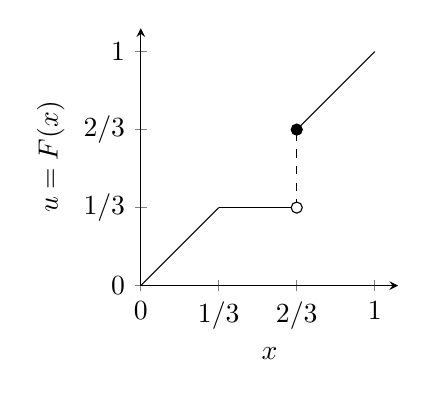
\begin{tikzpicture}
    \begin{axis}[
    axis lines=left,
    xlabel = $x$, ylabel = {$u = F(x)$},
    xmax = 1.1, xtick = {0, 1/3, 2/3, 1}, 
    ymax = 1.1, ytick = {0, 1/3, 2/3, 1},
    xticklabels={$0$, $1/3$, $2/3$, $1$},
    yticklabels={$0$, $1/3$, $2/3$, $1$}, 
    width=0.4\textwidth, height=0.4\textwidth]
    \addplot[domain=0:1/3] {x};
    \addplot[domain=1/3:2/3] {1/3};
    \addplot[domain=2/3:1] {x};
    \addplot[mark=*,only marks] coordinates {(2/3,2/3)};
    \addplot[mark=*,fill=white,only marks] coordinates {(2/3,1/3)};
    \draw [dashed] (2/3,1/3) -- (2/3,2/3);
    \end{axis}
\end{tikzpicture}
\captionof{figure}{An example of distribution function.}
\end{center}
The inverse $F^{-1}(u)$ is shown below
\begin{center}
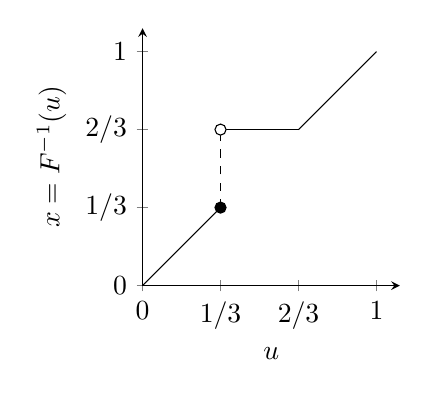
\begin{tikzpicture}
    \begin{axis}[
    axis lines=left,
    xlabel = $u$, ylabel = {$x = F^{-1}(u)$},
    xmax = 1.1, xtick = {0, 1/3, 2/3, 1}, 
    ymax = 1.1, ytick = {0, 1/3, 2/3, 1},
    xticklabels={$0$, $1/3$, $2/3$, $1$},
    yticklabels={$0$, $1/3$, $2/3$, $1$}, 
    width=0.4\textwidth, height=0.4\textwidth]
    \addplot[domain=0:1/3] {x};
    \addplot[domain=1/3:2/3] {2/3};
    \addplot[domain=2/3:1] {x};
    \addplot[mark=*,only marks] coordinates {(1/3,1/3)};
    \addplot[mark=*,fill=white,only marks] coordinates {(1/3,2/3)};
    \draw [dashed] (1/3,1/3) -- (1/3,2/3);
    \end{axis}
\end{tikzpicture}

\captionof{figure}{The psuedo-inverse of the previous example}
\end{center}
\end{example}

Now we turn to the problem of determining $f_\eta(y)$. Let us suppose that the range of $\xi$ is a (finite or infinite) open interval $I = (a,b)$, and that the function $\varphi = \varphi(x)$, with domain $(a,b)$, is continuously differentiable and either strictly increasing or strictly decreasing. We also suppose that $\varphi'(x) \ne 0, x\in I$. Let us write $h(y) = \varphi^{-1}(y)$ and suppose for definiteness that $\varphi$ is strictly increasing. Then when $y \in \varphi(I)$,
\begin{align*}
    F_\eta(y) = \p(\eta \le y) = \p(\varphi(\xi) \le y) = \p(\xi \le \varphi^{-1}(y)) &= \p(\xi \le h(y))
    = \int_{-\infty}^{h(y)}f_\xi(x)\, \d x
    = \int_{-\infty}^y f_\xi(h(z))h'(z)\, \d z.
\end{align*}
Therefore,
\begin{equation}
    f_\eta(y) = f_\xi(h(y))h'(y).
\end{equation}
Similarly, if $\varphi(x)$ is strictly decreasing,
\begin{equation}
    f_\eta(y) = f_\xi(h(y))(-h'(y)).
\end{equation}
Hence in either case
\begin{equation}
    f_\eta(y) = f_\xi(h(y))|h'(y)|.
\end{equation}
\begin{example}
If $\eta = a\xi + b, a\ne 0$, we have
\begin{equation}
    h(y) = \frac{y-b}{a} \quad \text{and} \quad f_\eta(y) = \frac{1}{|a|}f_\xi\bigg(\frac{y-b}{a} \bigg).
\end{equation}
\end{example}
If $\varphi = \varphi(x)$ is neither strictly increasing nor strictly decreasing, the above formula is inapplicable. However, the following generalisation suffices for many applications.
\begin{lemma}
Let $\varphi = \varphi(x)$ be defined on the set $\sum_{k=1}^n[a_k, b_k]$, continuously differentiable and either strictly increasing or strictly decreasing on each open interval $I_k = (a_k, b_k)$, and with $\varphi'(x) \ne 0$ for $x \in I_k$. Let $h_k = h_k(y)$ be the inverse of $\varphi(x)$ for $x \in I_k$, Then
\begin{equation}
    f_\eta(y) = \sum_{k=1}^n f_\xi(h_k(y))|h_k'(y)|\cdot I_{D_k}(y),
\end{equation}
where $D_k$ is the domain of $h_k(y)$.
\end{lemma}
\begin{example}
Let $\eta = \xi^2$ and take $I_1 = (-\infty, 0), I_2 = (0, \infty)$, and find that $h_1(y) = -\sqrt{y}, h_2(y) = \sqrt{y}$, and therefore
\begin{equation}
    f_\eta(y) = 
    \begin{cases}
     \frac{1}{2\sqrt{y}}[f_\xi(\sqrt{y}) + f_\xi(-\sqrt{y})], & y>0,\\
     0, & y\le 0.
    \end{cases}
\end{equation}
In particular, if $\xi \sim N(0,1)$,
\begin{equation}
    f_{\xi^2}(y) = 
    \begin{cases}
     \frac{1}{\sqrt{2\pi y}}e^{-y/2}, & y>0,\\
     0, & y\le 0.
    \end{cases}
\end{equation}
A straightforward calculation shows that
\begin{equation}
    f_{|\xi|}(y) = 
    \begin{cases}
     f_\xi(y) + f_\xi(-y), & y>0,\\
     0, & y\le 0.
    \end{cases}
\end{equation}
\begin{equation}
    f_{\sqrt{|\xi|}}(y) = 
    \begin{cases}
     2y(f_\xi(y^2) + f_\xi(-y^2)), & y>0,\\
     0, & y\le 0.
    \end{cases}
\end{equation}
\end{example}
Let $\xi$ and $\eta$ be random variables with joint distribution $F_{\xi, \eta}(x,y)$, and $\varphi = \varphi(x,y)$ be a Borel function, then 
\begin{equation}
    F_{\varphi(\xi, \eta)} (z) = \int_{\{ x,y: \varphi(x,y) \le z \}} \d F_{\xi,\eta}(x,y).
\end{equation}

\red{Plan: Should we also include some discussion about multivariable transformations?}

\subsection{Independent and Uncorrelated Random Variables}
\subsubsection{Independence}

\begin{definition}[(Mutual) Independence] Let $(\Omega,\F,\p)$ be a measure space.
\begin{itemize}
\item Assume there are events $A_1, A_2, ...$. The finite collection of events $\set{A_1, ..., A_n}$ is independent if $\p\bracket{\cap_{i=1}^n A_n} = \prod_{i=1}^n \p(A_i)$. The infinite collection $\set{A_1,...}$ is (mutually) independent if any finite sub-collections is independent. \\
\item Assume $\F_1, \F_2, ...$ are sub-$\sigma$-algebras of $\F$. Then the collection of sub-$\sigma$-algebras $\set{\F_1, \F_2, ...}$ is mutually independent if for any $A_1 \in \F_1, A_2 \in \F_2, ...$, we have $\p\bracket{\cap_{i=1}^n A_n} = \prod_{i=1}^n \p(A_i)$. The infinite collection $\set{\F_1,...}$ is (mutually) independent if any finite sub-collections is independent.
\item Let $\xi_1, \xi_2, ...$ be random variables on $(\Omega, \F, \p)$. Then the collection $\set{\xi_1, \dots, \xi_n}$ is (mutually) independent if the sub-$\sigma$-algebras $\sigma(\xi_1), ..., \sigma(\xi_n)$ are independent. In particular if $B_1, \dots, B_n \in \B(\R)$, then
\begin{equation*}
    \p(\xi_1 \in B_1,\dots, \xi_n \in B_n) = \prod_{i=1}^n \p(\xi_i \in B_i) = \p_{\xi_i}(B_i).
\end{equation*}
The definition can be extended to the infinite case as above.
\end{itemize}
\end{definition}

\begin{remark}
As seen in elementary probability classes, there is another notion of independence. Let's say there are events $A_1, A_2, ...$, then the collection of events $\set{A_1, ..., A_n}$ is \textit{pairwise} independent if for all $i,j$ with $i \neq j$ we have $\p(A_i \cap A_j) = \p(A_i) \p(A_j)$. It is clear that mutual independence implies pairwise independence but not vice-versa. There are similar notions when considering collections of sub-$\sigma$-algebra or random variables. Note that the notion of mutual independence is far more applicable than the notion of pairwise independence in probability theory. 
\end{remark}

Let us note the following shortcut in establishing mutual independence of sub-$\sigma$-algebra (and hence random variables).

\begin{lemma} \label{lem:independence_shortcut}
Let's say $\F_i = \sigma(\cC_i)$ for some $\pi$-system containing $\Omega$ (that are closed under finite intersection, see theorem \ref{thm:measure_determining}). If we know that for any $C_i \in \cC_i$ (with $\F_i$ belongs to an arbitrary finite sub-collection), $\p(\cap_{i=1}^n C_i) = \prod_{i=1}^n \p(C_i)$, then $\F_1, \F_2,...$ are independent.
\end{lemma}

\begin{proof}
It suffices to consider the case when there are only two $\sigma$-algebra in our collection, denoted as $\set{\F_i := \sigma(\cC_i)}_{i=1,2}$. We break the proof into two steps: 
\begin{itemize}
\item Fix $A \in \cC_1$ and consider the measures $Q_{1,A}(B) := \p(A \cap B)$ and $Q_{2,A}(B) := \p(A) \p(B)$ on $\cC_2$. Since these two measures agree on $\cC_2$, we know from theorem \ref{thm:measure_determining} that for all $A \in \cC_1$ we have $Q_{1,A} = Q_{2,A}$.
\item Now let $B \in \textcolor{blue}{\F_2}$ and consider the measures $\tilde{Q}_{1,B}(A) := \p(B \cap A)$ and $\tilde{Q}_{2,B}(A) := \p(B) \p(A)$. As seen in the above step, these two measures agree on $\cC_2$, so by theorem \ref{thm:measure_determining} we know that for all $B \in \cC_2$ we have $\tilde{Q}_{1,B} = \tilde{Q}_{2,B}$. This completes the proof.
\end{itemize}
\end{proof}

As an immediate corollary, we know that
\begin{corollary}
A necessary and sufficient condition for the random variables $\xi_1, \xi_2, \dots,\xi_n$ to be independent is that
\begin{equation}
    F_\xi(x_1,x_2,\dots,x_n) = F_{\xi_1}(x_1)\dots F_{\xi_n}(x_n)
\end{equation}
for all $(x_1,\dots, x_n)\in \R^n$.
\end{corollary}

\begin{proof}
This comes from the fact that the Borel sets are generated by the collection of left-half-intervals $(-\infty,a]$ and $\R$, with this collection being a $\pi$-system.
\end{proof}

Combining with Fubini-Tonelli theorem, we have
\begin{corollary}
If $\xi = (\xi_1, \dots, \xi_n)$ has a density $f_\xi$, then each $\xi_i$ has a density $f_{\xi_i}$. Furthermore, $\xi_1, \dots, \xi_n$ are independent if and only if 
\begin{equation}
    f_\xi(x_1, x_2, \dots, x_n) = f_{\xi_1}(x_1)\cdots f_{\xi_n}(x_n)
\end{equation}
for all $(x_1, \dots , x_n)$ except possibly for a Borel subset of $\R^n$ with Lebesgue measure zero.
\end{corollary}

\begin{corollary}
If $\xi_1,\dots, \xi_n$ are independent and $\xi_i$ has density $f_{\xi_i}$, $i = 1,\dots, n$, then $\xi$ has a density $f_\xi$ given by
\begin{equation*}
    f_\xi(x_1, x_2, \dots, x_n) = f_{\xi_1}(x_1)\cdots f_{\xi_n}(x_n).
\end{equation*}
\end{corollary}

\begin{remark}
Note that if $\xi_1,\dots, \xi_n$ each have a density, it does not follow that $(\xi_1,\dots, \xi_n)$ has a density.
\end{remark}

\subsubsection{Convolution of Independent Random Variables}
Let $\xi, \eta$ be two independent random variables, so $F_{(\xi,\eta)} (x,y)= F_\xi(x) F_\eta(y)$. Consider the random variable $\xi + \eta$. We get
\begin{align*}
    F_{(\xi,\eta)}(z) &= \int_{\{x,y:x+y \le z \}} \d F_\xi(x) \cdot \d F_\eta(y)\\
    &=\int_{\R^2}\chi_{x+y\le z} \, \d F_\xi(x) \cdot \d F_\eta(y)\\
    &=\int_{-\infty}^\infty \, \d F_\xi(x) \bigg\{ \int_{-\infty}^\infty \chi_{x+y \le z} \, \d F_\eta(y) \bigg\}\\
    &=\int_{-\infty}^\infty F_{\eta}(z-x) \, \d F_\xi(x)
\end{align*}

and similarly 
\begin{equation*}
    F_{(\xi,\eta)}(z) = \int_{-\infty}^\infty F_{\xi}(z-y) \d F_\eta(y).
\end{equation*}

Thus we obtained the following result
\begin{proposition}
The distribution function $F_{\xi + \eta}$ of the sum of two independent random variables is the convolution of their distribution functions. 
\begin{equation}
    F_{(\xi,\eta)}(z) = F_\xi * F_\eta = \int_{-\infty}^\infty F_{\xi}(z-y) \d F_\eta(y) = \int_{-\infty}^\infty F_{\eta}(z-x) \d F_\xi(x).
\end{equation}
\end{proposition}

Similarly, we can easily obtain
\begin{corollary}
If $\xi, \eta$ are independent a.c. random variables, then the density $f_{\xi + \eta}$ is the convolution of the densities.
\begin{equation}
    f_{\xi + \eta} = f_\xi * f_\eta = \int_{-\infty}^\infty f_{\xi}(z-y) f_\eta(y) \d y = \int_{-\infty}^\infty f_{\eta}(z-x) f_\xi(x)\d x.
\end{equation}
\end{corollary}

\begin{example}[$\xi, \eta$ - independent a.c. random variables]
\begin{itemize}
    \item[]
    \item Let $\xi \sim N(m_1,\sigma_1^2)$ and $\eta \sim N(m_2,\sigma_2^2)$, i.e.
    \begin{equation*}
        f_\xi(x) = \frac{1}{\sigma_1}\varphi\bigg(\frac{x-m_1}{\sigma_1} \bigg), \quad f_\eta(x) = \frac{1}{\sigma_2}\varphi\bigg(\frac{x-m_2}{\sigma_2} \bigg),
    \end{equation*}
    where
    \begin{equation*}
        \varphi(x) = \frac{1}{\sqrt{2\pi}}e^{-x^2/2}.
    \end{equation*}
    Then
    \begin{equation*}
        f_{\xi + \eta}(z) = \int_{-\infty}^\infty f_{\eta}(z-x)f_\xi(x)\d x = \frac{1}{\sqrt{\sigma_1^2 + \sigma_2^2}}\varphi \bigg( \frac{z - (m_1 + m_2)}{\sqrt{\sigma_1^2+\sigma_2^2}} \bigg).
    \end{equation*}
    Thus the sum of two independent normal random variables is the normal random variable $N(m_1 + m_2, \sigma_1^2 + \sigma_2^2)$. 
    \item Let $\xi_1, \xi_2, \dots \xi_n$ be independent $N(0,1)$. Then
    \begin{equation*}
        f_{\xi_1^2 + \cdots + \xi_n^2}(x) = 
        \begin{cases}
         \frac{1}{2^{n/2}\Gamma(n/2)}x^{(n/2)-1}e^{-x/2}, & x>0,\\
         0, &x\le 0.
        \end{cases}
    \end{equation*}
    The random variable $\xi_1^2 + \cdots + \xi_n^2$ is usually denoted by $\chi_n^2$ and its distribution is the $\chi^2$-distribution with $n$ degrees of freedom.
\end{itemize}
\end{example}

\begin{proposition}
Let $\xi$ and $\eta$ be independent random variables with $\E[\xi]<\infty$, $\E[\eta] < \infty$. Then $\E[\xi \eta] < \infty$ and $\E[\xi \eta] = \E[\xi] \E[\eta]$.
\end{proposition}

\begin{proof}
We utilise the four-step proofs. First assume $\xi, \eta \ge 0$. Consider
\begin{equation*}
    \xi_n = \sum_{k=0}^\infty \frac{k}{n}\chi_{\{\frac{k}{n} \le \xi(\omega) < \frac{k+1}{n}\}},
\end{equation*}
\begin{equation*}
    \eta_n = \sum_{k=0}^\infty \frac{k}{n}\chi_{\{\frac{k}{n} \le \eta(\omega) < \frac{k+1}{n}\}}.
\end{equation*}
Then $\xi_n \le \xi, \eta_n \le \eta$, $|\xi - \xi_n|\le \frac{1}{n}, |\eta - \eta_n|\le \frac{1}{n}$ for all $n$. Since $\xi, \eta$ are integrable, by dominated convergence theorem
\begin{equation*}
    \lim_{n\rightarrow \infty} \E[\xi_n] = \E[\xi], \quad \lim_{n\rightarrow \infty} \E[\eta_n] = \E[\eta].
\end{equation*}
Now write
\begin{align*}
    \E[\xi_n \eta_n] &= \sum_{i,j \ge 0} \frac{jk}{n^2}\E[\chi_{\{ \frac{j}{n} \le \xi < \frac{j+1}{n}\}} \chi_{\{ \frac{k}{n} \le \eta < \frac{k+1}{n}\}}] \quad \text{(Monotone Convergence)}\\
    &= \sum_{i,j \ge 0} \frac{jk}{n^2} \E[\chi_{\{ \frac{j}{n} \le \xi < \frac{j+1}{n}\}}] \E[\chi_{\{ \frac{k}{n} \le \eta < \frac{k+1}{n}\}}]  \quad \text{(Independence)}\\
    &=\E[\xi_n]\E[\eta_n]
\end{align*}
Since 
\begin{equation*}
    |\E[\xi\eta]-\E[\xi_n \eta_n]| \le \E[|\xi \eta - \xi_n \eta_n|] = \E[|\xi(\eta - \eta_n)+ \eta_n(\xi - \xi_n)|] \le \frac{1}{n}\E[|\xi|]+\frac{1}{n}\E\bigg[|\eta|+\frac{1}{n}\bigg] \rightarrow 0
\end{equation*}
as $n \rightarrow \infty$, we have that
\begin{equation*}
    \E[\xi \eta] = \lim_{n \rightarrow \infty} \E[\xi_n \eta_n] = \lim_{n \rightarrow \infty} \E[\xi_n] \lim_{n \rightarrow \infty}\E[\eta_n] = \E[\xi] \E[\eta],
\end{equation*}
and $\E[\xi \eta] < \infty$. The result in the general case follows by using the representation $$\xi = \xi^+ - \xi^-, \eta = \eta^+ - \eta^-.$$
\end{proof}

In fact, we can prove a stronger converse
\begin{proposition} \label{prop:independence_by_product}
Under the above setting, $\xi,\eta$ are independent iff for all Borel-measurable functions $f,g$ we have $\E[f(\xi) g(\eta)] = \E[f(\xi)] \E[g(\eta)]$.
\end{proposition}

\begin{hint}
For $(\Leftarrow)$ we directly apply the assumption for $f = \chi_{A_1}, g = \chi_{A_2}$, such that $A_1 = \xi_1^{-1}(B_1)$ for an arbitrary $B_1 \in \B(\R)$ and similarly for $A_2$. For $(\Rightarrow)$ we utilise the four-step proof similar to above.
\end{hint}

\subsubsection{Correlation}
We also define another notion of "unrelatedness" of two random variables. First we define the notion of \textbf{covariance}:

\begin{definition}[Covariance]
Let $\xi, \eta$ be a pair of random variables on the same probability space. Their \textbf{covariance} is
\begin{equation}
    \cov[\xi, \eta] := \E[(\xi - \E[\xi])(\eta - \E[\eta])].
\end{equation}
if the expectation above exists.
\end{definition}
\begin{remark}
Note that 
\begin{equation*}
    \V[\xi + \eta] = \V[\xi] + \V[\eta] + 2\cov[\xi, \eta],
\end{equation*}
so 
\begin{equation*}
    \cov[\xi, \eta] = 0 \implies \V[\xi + \eta] = \V[\xi] + \V[\eta].
\end{equation*}
\end{remark}

\begin{definition}[Uncorrelated variables]
The random variables $\xi$ and $\eta$ are called \textbf{uncorrelated} if $$\cov[\xi, \eta] = 0.$$
\end{definition}

\begin{corollary} \label{cor:independence_uncorrelated}
Independent random variables are uncorrelated.
\end{corollary}
\begin{proof}
Indeed, using the theorem from above,
\begin{equation*}
    \cov[\xi, \eta] = \E[\xi \eta] - \E[\xi]\E[\eta] = 0.
\end{equation*}
\end{proof}
The converse is not true. 

\begin{example}
    Consider for example the random variable $\alpha$ which takes the values $0,\frac{\pi}{2}, \pi$ with probability $\frac13$. Then $\xi = \sin{\alpha}, \eta = \cos{\alpha}$ are uncorrelated ($\E[\xi] = \frac13, \E[\eta] = 0$), but they are not independent since
    \begin{equation*}
        \p(\xi = 1, \eta = 1) = 0 \ne \frac19 = \p(\xi = 1)\p(\eta = 1).
    \end{equation*}
    Indeed we can also see that the random variables $\xi, \eta^2$ are correlated, since $\E[\eta^2] = 2/3$ and $\E[\xi] \E[\eta+1] = 2/9$, but $\cov[\xi, \eta^2] = -2/9$.
\end{example}

% might add some remarks on independence of moments
\newpage

\part{Concepts of Convergence}
\section{Coin Flips: Convergence in Probability}
We now have sufficient tools from measure theory to get into the first serious topic of probability - limiting theorems. Given a random sequence $(\xi_1, \xi_2, \dots)$ with $\xi_i$ \textit{independently and identically distributed} (i.i.d.), we would like to study the deviation between the empirical mean (or time average) $S_n/n$ (with $S_n = \xi_1 + \dots + \xi_n$) and the actual mean $\E[\xi_1]$ (space average). In particular, do we know anything when $n \to \infty$?\\

In this chapter, we consider our simplest example of random events: flipping $n$ independent unfair coins.

\subsection{Constructing the sample space}
So how do we represent the flipping of $n$ independent unfair coins in the mathematical framework we have built in the previous sections? Let us consider the case of flipping just one coin. Assume the outcomes are 0 and 1 with probability of getting 1 being $p \in (0,1)$. We hope to express this as a random variable $\xi$ with value in $\set{0,1}$ on suitable probability space $(\Omega, \A, \p)$, such that $\p_\xi(\set{0}) = 1-p$ and $\p_\xi(\set{1}) = p$. A more elaborate way to write the above condition is: 
\begin{equation} \label{eq:Bernoulli_pmf}
    \p_\xi(\set{x}) = p^x (1-p)^{1-x}, \quad x = 0,1
\end{equation}
There are several choices of sample spaces we can choose: \\

\begin{itemize}
    \item The natural choice: 
    $$\Omega = \set{0,1}, \; \A = 2^\Omega, \; \p(\set{\omega}) = p^\omega (1-p)^{1-\omega}, \; \xi(\omega) = \omega$$
    \item A more complicated choice: 
    $$\Omega = [0,1], \; \A = \B([0,1]), \; \p(E) = \Leb(E), \; \xi(\omega) = \chi_{(p,1]}(\omega)$$
    with $\lambda$ being the Lebesgue measure. This represents how a computer simulates a flipping of biased coin: first generate a random number $r \in [0,1]$ from uniform distribution (using e.g. the \verb|numpy.random.rand| function in Python), then return $0$ if $r < 1-p$ and $1$ otherwise. 
\end{itemize}

In both cases we see that $\p_\xi(\set{0}) = 1-p$ and $\p_\xi(\set{1}) = p$. In fact, we have shown from LOTUS (theorem \ref{thm:LOTUS}) that the distribution functions (hence expectation etc.) will not depend on our choice of probability spaces and random variables, as long as $\p_\xi$ satisfies \eqref{eq:Bernoulli_pmf}.\\

How can we extend to the experiment of flipping $n$ coins? The wrong way is to assume that $\xi_1, ..., \xi_n$ are on the same sample space $(\Omega, \A, \p)$ such that $\xi_1= ...= \xi_n$, since these random variables really mean flipping a single coin once and recording the result $n$ times. (In particular the random variables are not independent for sure). In fact, it will be hard to write down a large number of independent random variables defined on any of the sample spaces $(\Omega, \A, \p)$ in the above example. \\

A standard way of describing $n$ independent coin flips (or $n$ independent trials in general) is to assume that the random variables $\xi_1, \xi_2, ..., \xi_n$ in different sample spaces (i.e. $\xi_1$ defines on $(\Omega_1, \A_1, \p_1)$, $\xi_2$ defines on $(\Omega_2, \A_2, \p_2)$ and so on...) However, we need a way to understand any operations involving more than one $\xi_i$'s. The way to mitigate is to consider the product space $(\Omega^{(n)}, \A^{(n)}, \p^{(n)}) = \otimes_{i=1}^n (\Omega_i, \A_n, \p_n)$. As a reminder, the sample space of this new probability space is 
\begin{equation*}
    \Omega^{(n)} = \Omega_1 \times ... \times \Omega_n = \set{\omega = (\omega_1,...,\omega_n) \,:\, \forall i, \; \omega_i \in \Omega_i},
\end{equation*}

the new collection of events are
\begin{equation*}
    \A^{(n)} = \sigma(\set{A_1 \times ... \times A_n \,:\, \forall i, \; A_i \in \A_i}) = 2^{\Omega^{(n)}}
\end{equation*}

and the new probability measures are $\p_n$ satisfying 
\begin{equation*}
    \p^{(n)}(A_1 \times ... \times A_n) = \prod_{i=1}^n \p_i(A_i)
\end{equation*}

Then we can define the family of projection function onto the $i$-th component,  $\proj^{(n)}_i: (\Omega^{(n)},\A^{(n)}) \to (\Omega_i, \A_i)$ such that $\proj^{(n)}_i(\omega_1, ..., \omega_n) = \omega_i$. For convenience, we drop the superscript $(n)$ if there is no ambiguity. Notice that the projection functions are measurable, since the preimage of any sets in $\A_i$ is 
$$\proj_i^{-1}(A_i) = \Omega_1 \times ... \times \Omega_{i-1} \times A_i \times \Omega_{i+1}, ..., \Omega_n \in \A^{(n)}$$

Now we can define new random variables $\tilde{\xi}:(\Omega^{(n)}, \A^{(n)}, \p^{(n)}) \to \set{0,1}$ such that $\tilde{\xi}_i(\omega) = \xi_i(\proj_i(\omega))$. These random variables are an accurate description of flipping $n$ coins since:
\begin{enumerate}
    \item The marginal distribution of $\xi_i$, defined as the measure $A \mapsto \p_{\tilde{\xi}_i}(\Omega_1 \times ... \times A \times ... \times \Omega_n)$ satisfies \eqref{eq:Bernoulli_pmf}.
    \item The family $(\tilde{\xi}_i)$ of random variables are independent.
\end{enumerate}

\begin{exercise}
Verify the above assertions.
\end{exercise}

Finally, we want to extend the above construction to $n \to \infty$, i.e. consider the space $(\Omega, \A) = \otimes_{i=1}^\infty (\Omega_i, \A_i)$ on a suitable probability measure $\p$, so that we can discuss large-sample theorems. We want the probability measure to satisfies:
\begin{equation} \label{eq:consistent_result}
    \p\bracket{A_1 \times ... \times A_n \times \Omega_{n+1} \times ...} = \prod_{i=1}^n \p_i(A_i)
\end{equation}

The good news is, such probability measure exists if we use $\Omega_i \equiv \Omega$ and $\A_i \equiv \A$ in our above examples. If we assume the natural choice, then we can safely set
\begin{equation*}
    \p(\set{(\omega_1,\omega_2,...)}) = \prod_{i=1}^\infty p^{\omega_i} (1-p)^{1-\omega_i} = p^{\sum \omega_i} (1-p)^{\sum (1-\omega_i)}
\end{equation*}
since the probability measure is well-defined for all singletons $\set{(\omega_1,\omega_2,...)}$. If we use the example when $\Omega_i = [0,1]$, we can check that our sequence of measures $(\p^{(n)})$ is consistent (see definition \ref{def:consistent_sequence}) and apply the Kolmogorov Extension Theorem (theorem \ref{thm:kolmogorov_extension}) to define $\p$.\\ 

Note the above construction can be generalised to describe a sequence of independent experiments. The above construction means that we need not worried about specifying a single probability space to describe a sequence of independent experiments. As a summary, \textbf{if we want to describe infinite sequence of experiment with underlying distribution $\p_\xi$, we consider the infinite product space $(\R, \B(\R))^{\otimes \infty}$ equipped with the probability measure $\p$ as determined by the Kolmogorov extension theorem, then the projections onto the $i$-th component $\proj_i$ are random variables with distribution $\p_\xi$.} From now on, we abuse notation by not mentioning the underlying probability space, dropping the tilde sign above $\xi$ and interpreting any operations (especially addition) in the above sense.\\

\subsubsection{Radamecher Functions}
There is a third way to construct a \textbf{fair} coin flip without using the Kolmogorov extension theorem. Consider the probability space $([0,1], \B([0,1]), \p)$ with $\p = \lambda$ being the Lebesgue measure. Consider the binary expansions $\omega = 0.\overline{\omega_1 \omega_2 \dots}_2$ of numbers $\omega \in \Omega$, and define random variables $\xi_1(\omega), \xi_2(\omega),\dots$ by putting $\xi_k(\omega) = \omega_k$. We extend these functions so that for all $k$, $\xi_i(1) = 1$. A neater way to express these random variables is: 
\begin{equation}
\xi_k(\omega) = H(\sin 2^k \pi t)
\end{equation}
where $H(t) = \chi_{[0,\infty)}$ is the heavyside function. Since, for all $n \ge 1$ and all $x_1,\dots, x_n$ taking a value $0$ or $1$, 
\begin{align*}
    \{\omega: \xi_1(\omega) = x_1, \dots, \xi_n(\omega) = x_n \} = \bigg\{ \omega: \frac{x_1}{2} + \frac{x_2}{2^2} + \cdots + \frac{x_n}{2^n} \le \omega < \frac{x_1}{2} + \cdots + \frac{x_n}{2^n} + \frac{1}{2^n} \bigg\},
\end{align*}
the $\p-$measure of this set is $\frac{1}{2^n} = \prod_{i=1}^n \p(\xi_n(\omega) = x_n)$. It follows that $\xi_1, \xi_2, \dots$ is a sequence of independent identically distributed random variables with 
\begin{equation*}
    \p(\xi_1 = 0) = \p(\xi_1 = 1) = \frac12.
\end{equation*}
As we will see in later chapters, such construction give rises to some important number theoretic results regarding binary expansion of numbers in $[0,1]$.


\subsection{Weak Law of Large Numbers}
\subsubsection{A high probability statement for coin flips}
Let $S_n = \xi_1 + \dots \xi_n$. Then 
\begin{equation*}
    \E[S_n] = \sum_{j=1}^n \E[\xi_n] = \sum_{j=1}^n(1 \cdot \p_{\xi_j}(\xi_j = 1) + 0\cdot \p_{\xi_j}(\xi_j = 0)) = np.
\end{equation*}
Thus the mean value of $S_n/n$ is equal to $p$. Our central question is: what does $|\frac{1}{n}S_n(\omega) - p|$ converges to for large $n$? Moreover, in what sense we can consider the convergence? It cannot be that
\begin{equation*}
    \bigg|\frac{S_n(\omega)}{n} - p\bigg| \rightarrow 0
\end{equation*}
uniformly/pointwise in $\omega$, because there is always an $\omega$ such that $\xi_i(\omega) = 1$ for all $i$, so $S_n(\omega)/n \equiv 1 \nrightarrow p$, so we must consider a weaker notion of convergence. Before delving into our discussion, let us recall the following observation

\begin{exercise}
Verify that $S_n \sim \sB(n,p)$. Hence show that $\norm{S_n/n - p}^2_{L^2} = \V[S_n/n] = p(1-p)/n \overset{n \to \infty}{\to} 0$.
\end{exercise}

This shows that, in fact, we have $L^2$ convergence. With more careful analysis we show that we actually have $L^p$ convergence for any $p \in [1,\infty)$. By Chebyshev inequality, we also shows that for all $\epsilon > 0$ (fixed)
\begin{equation} \label{eq:Bernoulli_Chebyshev}
    \p\bracket{\abs{\frac{S_n}{n} - p} > \epsilon} \leq \frac{\V[S_n/n]}{\epsilon^2} = \frac{p(1-p)}{n\epsilon^2}
\end{equation}

So for all $\epsilon > 0$ fixed, we can always make the probability $\p\bracket{\abs{S_n/n - p} > \epsilon}$ arbitrary small by choosing sufficiently large $n$. This is known as \textit{convergence of probability}.\\

\begin{unexaminable}
\begin{remark}
*We can make \eqref{eq:Bernoulli_Chebyshev} sharper by considering Chernoff bound. Indeed, we know that the random variable $S_n$ has moment generating function
\begin{equation}
    M_{S_n}(t) = (1-p+pe^t)^n, \quad \forall t \in \R
\end{equation}

so from Chernoff bound, we know for all $t>0$ we have
\begin{align*}
    \p\bracket{\frac{S_n}{n} - p > \epsilon} &= \p\bracket{\exp(t(S_n - np)) > \exp(tn\epsilon)} \\
    &\leq \frac{\exp(-tnp)\E[\exp(tS_n)]}{\exp(tn\epsilon)} \\
    &= \exp\bracket{n \bracket{\ln(1-p+pe^t) - t(p+\epsilon)}} =: \exp(n(\phi(t)-t\epsilon))
\end{align*}
where $\phi(t):= \ln(1-p+pe^t) - pt$. We claim is that $\phi(t)$ is bounded by a quadratic function. We can prove this by bounding the second derivative of $\phi(t)$. Note that
\begin{gather}
    \phi'(t) = -p + \frac{pe^t}{1-p+pe^t} = 1-p-\frac{1-p}{1-p+pe^t} \\
    \phi''(t) = \frac{(1-p)pe^t}{(1-p+pe^t)^2} = \frac{1-p}{1-p+pe^t}\bracket{1-\frac{1-p}{1-p+pe^t}}
\end{gather}
Let $\displaystyle{u(t) = \frac{1-p}{1-p+pe^t}}$. Then clearly $\forall t, \, 0 < u(t) < 1$. Moreover, we see that $\phi''(t) = u(1-u) = -(u-1/2)^2 + 1/4$. Therefore we know for all $t$, $\phi''(t) \in (0,1/4]$. Hence by Taylor Theorem, there exists a $c$ between $0$ and $t$ such that
\begin{equation}
    \phi(t) = \phi(0) + t\phi'(0) + \frac{t^2}{2}\phi''(c) \leq \frac{t^2}{8} 
\end{equation}
Substitute into our Chernoff bound yields
\begin{equation}
    \p\bracket{\frac{S_n}{n} - p > \epsilon} \leq \exp(n(t^2/8 - \epsilon t)) = \exp(n((t-4\epsilon)^2/8 - 2\epsilon^2))
\end{equation} 
So by choosing $t = 4\epsilon$ (such that the RHS) is minimised we yield a much sharper bound:
\begin{equation}
    \p\bracket{\frac{S_n}{n} - p > \epsilon}  \leq \exp(-2n\epsilon^2)
\end{equation}
By symmetry we also obtain 
\begin{equation} \label{eq:Bernoulli_hoeffding}
    \p\bracket{\abs{\frac{S_n}{n} - p} > \epsilon} \leq 2\exp(-2n\epsilon^2)
\end{equation}
We obtain a much sharper bound than \eqref{eq:Bernoulli_Chebyshev} since we now have exponential decay rather than a quadratic decay. The trick of isolate the term $-nt\epsilon$ and bounding $\phi(t)$ by a quadratic function is common, since this can be generalised with any random variables $S_n \in L^\infty(\Omega)$. Such a bound is called a \textit{Hoeffding bound}, and we will discuss that further in latter chapter.
\end{remark}
\end{unexaminable}

\subsubsection{$L^2$ Weak Law of Large Numbers}
Let us study how the weak law of large numbers can be generalised. We first formally define the definition of convergence in probability. The definition holds for not only real-valued random variables, but also random variables taking values in a Polish space $(X,\B(X))$ (equipped with the Borel $\sigma$-algebra) associated with a metric $d$. Recall that a metric space is Polish if it is complete and separable (see remark \ref{rmk:PolishSpace}). 
\begin{definition}
A sequence $\xi_1, \xi_2, \dots $ of random variables from probability space $(\Omega,\F,\p)$ to Polish space $(X,\B(X))$ with metric $d$ converges \textit{in probability}, or \textit{in measure $\p$}, to the random variable $\xi$ (denoted by $\xi_n \xrightarrow{p} \xi$) if for every $\varepsilon > 0$
\begin{equation*}
    \p(d(\xi_n, \xi) > \varepsilon) \rightarrow 0, \quad n\rightarrow \infty.
\end{equation*}
\end{definition}

\begin{exercise}[Properties of convergence in probability]
Let $(\xi_i)_{i\geq 1}$, $(\eta_i)_{i \geq 1}$ are sequences of random variables on $(\Omega,\F,\p)$, and also let $\xi$, $\eta$ be random variables on $(\Omega,\F,\p)$
\begin{enumerate}
    \item Check that the limit of convergence in probability is almost surely unique: if $\xi_i$ converges in probability to $\xi$ and $\xi'$ then $\xi = \xi'$ almost surely.
    \item Prove that if $\xi_i \overset{p}{\to} \xi$ and $\eta_i \overset{p}{\to} \eta$ then for all real numbers $a,b$ we have $a\xi_i + b\eta_i \overset{p}{\to} a\xi + b\eta$.
    \item Prove that if $\xi_i \overset{p}{\to} \xi$ and $\eta_i \overset{p}{\to} \eta$ then for all real numbers $a,b$ we have $\xi_i \eta_i \overset{p}{\to} \xi \eta$. Notice this is not necessary true if we have $L^p$ convergence. What's wrong with the argument, and can we refine the statements?
    \item (Slutsky's lemma) Show that if $\xi_i \xrightarrow{p} \xi$ and $\eta_i \xrightarrow{p} \eta$ and if $\varphi(x,y)$ is a continuous function, then 
    \begin{equation*}
        \varphi(\xi_i, \eta_i) \xrightarrow{p} \varphi(\xi, \eta).
    \end{equation*}
\end{enumerate}
\end{exercise}

Note that by Markov inequality that if $\xi_n \to \xi$ in $L^p$ ($p\geq 1$, see definition \ref{def:Lp_convergence}), then we must have $\xi_n \xrightarrow{p} \xi$, because
\begin{equation}
    \p(|\xi_n - \xi| > \varepsilon) \leq \frac{\norm{\xi_n - \xi}_{L^p}^p}{\varepsilon^p} \to 0
\end{equation}

Let $\xi_1, \dots, \xi_n$ be a random variables. Denote
\begin{equation*}
    S_n^{(c)} = \sum_{j=1}^n (\xi_j - \E[\xi_j]).
\end{equation*}
Note $\E[S_n^{(c)}] = 0$. How can we fully use Chebyshev inequality to make the assumptions on $\xi_1,...,\xi_n$ as weak as possible? For simplicity, we first assume $\xi_i \in L^2$ such that $\V[\xi_i] \leq C$ for some constant $C$ independent of $i$. Then, if we assume that $\xi_1,...,\xi_n$ are pairwise uncorrelated (which is a much weaker assumption than independence), then we have 
\begin{equation}
    \V[S_n] = \sum_{i=1}^n \V[\xi_i] \leq Cn
\end{equation}

and hence we have the following 

% \begin{remark}
% \begin{align*}
%     \p \bigg( \bigg|\frac{S_n}{n} - p \bigg| > \epsilon \bigg) &= \sum_{k : |\frac{k}{n} - p|\ge \varepsilon} \p(S_n = k)
% \end{align*}
% concentrated at $k \sim n p!$. 
% \end{remark}

\begin{theorem}[$L^2$ Weak Law of Large Numbers] \label{thm:WLLN2}
Let $\xi_1, \dots, \xi_n$ be uncorrelated $L^2$ random variables such that $\V[\xi_j] \le C$ for some $C > 0$ and all $n \ge 1$. Then $S_n^{(c)}/n \xrightarrow{p} 0$
\end{theorem}
\begin{proof}
By Chebyshev's inequality and since $\xi_j$ are uncorrelated, for all $\epsilon > 0$
\begin{equation}
    \p  \bigg(\bigg|\frac{S_n^{(c)}}{n}\bigg| > \varepsilon\bigg) \leq \frac{\V[S_n^{(c)}/n]}{\varepsilon^2} \leq 
    \frac{C}{n \varepsilon^2} \overset{n \to \infty}{\to} 0
\end{equation}
\end{proof}

% More examples
% Monte-carlo integration
% Weierstrass Approximation Theorem

\subsubsection{Weak Law of Large Number for uniformly integrable sequences*}
\begin{unexaminable}
Can we try to weaken the assumption that $\xi \in L^2$, to say, $\xi \in L^1$?
\end{unexaminable}

\subsection{Local and Central Limit Theorem}
We now return to our coin flipping scenario. Recall we have $S_n = \xi_1 + \xi_2 + \cdots + \xi_n$, where $\xi_j$ are iid as $\mathsf{B}(1,p)$ as constructed in section 4.1. As discussed in previous section, $S_n$ tends to be close to $np$ for large $n$. 
\begin{center}
    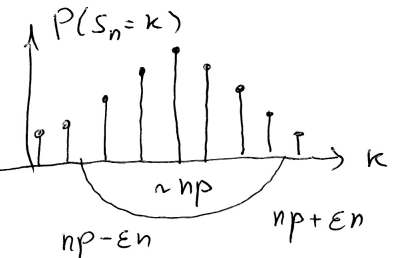
\includegraphics[scale=0.8]{sa.png}
\end{center}

Specifically, let us take some interval $\I_n = (n(p-\varepsilon), n(p+\varepsilon))$. If we pick some sufficiently large $\varepsilon$, say $\varepsilon = n^{\alpha}$ where $\alpha > 1/2$, then by Chebyshev inequality  \eqref{eq:Bernoulli_Chebyshev} (or Hoeffding bound \eqref{eq:Bernoulli_hoeffding}) we know that
\begin{equation} \label{eq:binomial_concentration}
\p(S_n \in \I_n^c) = \p(|S_n/n - p| > n^{\alpha - 1}) \leq \frac{p(1-p)}{n^{1+2\alpha - 2}} = \frac{p(1-p)}{n^{2\alpha - 1}} \overset{n \to \infty}{\to} 0
\end{equation}

and the decaying bounds of $\p(S_n \in \I_n^c)$ no longer exist when $\alpha \leq 1/2$. How much do we know about $\p(S_n \in \I_n^c)$ for this case? Will it tends to some non-trivial constant in $(0,1)$, or will it increase and tend to $1$? We will see that the central limit theorem shows that at the boundary case $\alpha = 1/2$, $\p(S_n \in \I_n^c)$ tends to some non-trivial constant in $(0,1)$ depending on the constant $C$ when defining $\varepsilon = C/n^{1/2}$. This also suggests that the rescaled mean $S_n/n^\alpha$ at the threshold $\alpha = 1/2$ will "converge" in some way to a non-trivial distribution.

\subsubsection{A crash course in asymptotic analysis}
Before we delve into the main discussions, we define two important order notations for sequences $f_n$:

\begin{definition}[Order notations] Consider two sequences $f_n, g_n$. As $n \to \infty$, we say that
\begin{itemize}
    \item (Big $O$) $g_n = O(f_n)$ if $|g_n/f_n|$ is bounded for sufficiently large $n$, i.e. there exists constant $C>0$ and $N$ such that for all $n \geq N$, $|g_n| \leq C|f_n|$
    \item (Small $o$) $g_n = o(f_n)$ if $|g_n/f_n| \to 0$ as $n \to \infty$. In other words, for all constants $\epsilon > 0$, there exists $N := N(\epsilon)$ such that for all $n \geq N$, $|g_n| \leq \epsilon |f_n|$. We also sometimes write $g_n \ll f_n$ or $f_n \gg g_n$.
    \item (Asymptotic equivalence) $g_n \sim f_n$ if $|g_n/f_n| \to 1$ as $n \to \infty$. Equivalently, we have $g_n = (1+o(1)) f_n$.
    \item (Order) $g_n = \Theta(f_n) = \ord(f_n)$ if $g_n = O(f_n)$ but $g_n$ is not $o(f_n)$.
\end{itemize}
\end{definition}

\begin{remark} \phantom{blah} 
\begin{itemize} 
    \item Notice the use of equal sign is an abuse of notation.
    \item The definitions can be extended to any functions $f(x)$ defined on real or complex numbers, in such case we can assume $x$ tends to some points $x_0$ including $\infty$.
    \item We can also consider order notations for sequences of functions. Let $g_n = g_n(\alpha)$, $f_n = f_n(\alpha)$. We say  $g_n(\alpha) = O(|f_n(\alpha)|)$ \textbf{uniformly} if above definition holds with constants $C,N$ independent of $\alpha$. We also have analogous definition for $g_n(\alpha) = o(|f_n(\alpha)|)$.
\end{itemize}
\end{remark}

With this, we can prove one of the most important result in asymptotic analysis
\begin{lemma}[Stirling's Approximation]
As $n \to \infty$, we have
\begin{equation}
    n! = \sqrt{2\pi n} \bracket{\frac{n}{e}}^n \bracket{1 + O(1/n)} 
\end{equation}
\end{lemma}

\begin{unexaminable}
\begin{proof} (Sketch)* There are many ways to prove this famous results, perhaps the quickest way is to notice that $n! = \Gamma(n+1)$, where $\Gamma(z)$ is the Gamma function satisfying
\begin{equation}
    \Gamma(z+1) = \int_0^\infty t^z e^{-t} \, dt = \int_0^\infty \exp(z \ln t - t) \, dt
\end{equation}
Apply a change of variable $s = t/z$, we have
\begin{equation}
    \Gamma(z+1) = \int_0^\infty t^z e^{-t} \, dt = z^{z+1}\int_0^\infty \exp(z(\ln s - s)) \, ds
\end{equation}
Notice the function $\phi(s)$ has the following Taylor series at $s = 1$:
\begin{equation}
    \ln s = \ln (1+(s-1)) = (s - 1) - \frac{(s-1)^2}{2} + O((s-1)^3)
\end{equation}
and therefore
\begin{equation}
    \Gamma(z+1) = z\bracket{\frac{z}{e}}^z \int_0^\infty \exp\bracket{-z \bracket{\frac{(s-1)^2}{2} + O(s-1)^3}} \, dz
\end{equation}
With careful analysis we see that the integral is equivalent to 
\begin{equation}
    \int_{-\infty}^\infty \exp\bracket{-z\frac{(s-1)^2}{2}} \, ds = \sqrt{\frac{2\pi}{z}}
\end{equation}
The main difference is that we now consider range of integration to be $(-\infty, \infty)$ instead of $[0,\infty)$ and ignore the higher order term, in both cases would introduce error which is exponentially small (so can be ignored). Hence we prove that
\begin{equation}
    n! \sim \sqrt{2\pi n} \bracket{\frac{n}{e}}^n
\end{equation}
Refining the analysis to incorporate the $O(1/n)$ correction is hard as it involves more advanced techniques in asymptotic analysis, so will not be included here.
\end{proof}
\end{unexaminable}

With this we can briefly sketch the asymptotic analysis of binomial coefficient. Let's say $n,k,n-k$ all tends to infinity (e.g. $k = np$ for $k \in (0,1)$), then we can use Stirling's formula to obtain
\begin{align*}
    {n\choose k} &= \frac{n!}{k! (n-k)!} \\
    &= \frac{\sqrt{n}}{\sqrt{2\pi k(n-k)}} \frac{(n/e)^n}{(k/e)^k ((n-k)/e)^{n-k}} \textcolor{violet}{\frac{1+O(1/n)}{(1+O(1/n))1+O(1/n)}}\\
    &= \frac{\sqrt{n}}{\sqrt{2\pi k(n-k)}}  \exp\bracket{n \ln n - k \ln k - (n-k) \ln (n-k)}\textcolor{violet}{\frac{1+O(1/n)}{(1+O(1/n))(1+O(1/n))}}
\end{align*}

We notice that the purple term only gives a correction of $1+O(1/n)$. Instead of going through careful analysis, we can build intuition by treating the $O(1/n)$ correction terms as being exactly equal to $1/n$. Then the denominator satisfies $(1+1/n)^{-2} = 1-2/n+... = 1+O(1/n)$. Then conclude that $(1+1/n)(1-2/n) = 1-1/n+... = 1+O(1/n)$. To sum up, we have
\begin{equation}
    {n\choose k} = \frac{\sqrt{n}}{\sqrt{2\pi k(n-k)}} \exp\bracket{n \ln n - k \ln k - (n-k) \ln (n-k)} \bracket{1+O\bracket{\frac{1}{n}}}
\end{equation}

\subsubsection{Proving the Central Limit Theorem}

We recall the following result regarding the probability mass function of a binomial distribution $\mathsf{B}(n,p)$:
\begin{exercise}[Monotonicity of Binomial probability] \label{ex:mono_of_bin_prob}
Show that $\p(S_n = k)$ is monotone in $k$ below and above its point of maximum.
\end{exercise}

With this we can prove the local limit theorem, which specifies the local asymptotics of probability mass distribution at the point $S_n = k$.

\begin{theorem}[Local Limit Theorem]
For any $0 < p < 1$,
\begin{equation}
    \max_{0 \le k \le n} \bigg|  \p(S_n = k) - \frac{1}{\sqrt{2 \pi p (1-p)} \sqrt{n}} e^{-\frac{x^2}{2p(1-p)}}  \bigg| = o\bigg(\frac{1}{\sqrt{n}}\bigg) \quad n \rightarrow \infty,
\end{equation}
where $\displaystyle{x = x_{k,n} := \frac{k-np}{\sqrt{n}}}$ 
\end{theorem}
\begin{proof}
The main subtlety is that we cannot always apply Stirling's formula. We have to first consider $k$ that are "sufficiently close" to $np$. Specifically, we consider $k$ such that
\begin{equation}
    |x_{k,n}| \leq \frac{A_n}{\sqrt{n}}, \quad A_n = n^\epsilon \; \text{with} \; \epsilon \in (0,1)
\end{equation}
Then we have $k = np+x\sqrt{n}$, $k$
\begin{gather*}
    k = np+x\sqrt{n} = np(1+O(A_n/n))\\
    n-k = n(1-p) - x\sqrt{n} = n(1-p)(1+O(A_n/n))
\end{gather*}
These inequalities ensure that both $k$ and $n-k$ tends to infinity as $n \to \infty$, and we can safely use Stirling's approximation to show that
\begin{align*}
    \p(S_n = k) = \textcolor{orange}{\underbrace{\frac{\sqrt{n}}{\sqrt{2\pi k(n-k)}}}_{\mathsf{(A)}}} \textcolor{violet}{\underbrace{\exp\bracket{n \ln n - k (\ln k - \ln p) - (n-k) (\ln (n-k) - \ln (1-p))}}_{\mathsf{(B)}}} \bracket{1+O\bracket{\frac{1}{n}}}
\end{align*}
We first analyse $\textcolor{orange}{\mathsf{(A)}}$: notice that
\orange{
\begin{align*}
    \mathsf{(A)} &= \frac{\sqrt{n}}{\sqrt{2\pi k(n-k)}} \\
    &= \frac{1}{\sqrt{2\pi np(1-p)(1+O(A_n/n))(1+O(A_n/n))}} \\
    &= \frac{1}{\sqrt{2\pi np(1-p)}} (1+O(A_n/n))
\end{align*}}
The the correction factor can be obtained using similar arguments above. We can then analyse $\textcolor{violet}{\mathsf{(B)}}$ by noticing that 
\textcolor{violet}{
\begin{align*}
    \mathsf{(B)} &= \exp\bracket{n \ln n - k\bracket{\ln n + \ln\bracket{1+\frac{x}{p\sqrt{n}}}} - (n-k)\bracket{\ln n + \ln\bracket{1-\frac{x}{(1-p)\sqrt{n}}}}} \\
    &= \exp\bracket{-\sqbracket{(np+x\sqrt{n}) \ln\bracket{1+\frac{x}{p\sqrt{n}}} + (n(1-p) - x\sqrt{n}) \ln\bracket{1-\frac{x}{(1-p)\sqrt{n}}}}} \\
    &= \exp\bigg( -\bigg[ np\bracket{\frac{x}{p\sqrt{n}} - \frac{x^2}{2p^2 n} + O\bracket{\frac{x^3}{n^{3/2}}} + \frac{x^2}{p} + O\bracket{\frac{x^3}{n^{1/2}}}} \\
    &\phantom{=}+ n(1-p) \bracket{-\frac{x}{(1-p)\sqrt{n}} - \frac{x^2}{2(1-p)^2 n} + O\bracket{\frac{x^3}{n^{3/2}}}} + \frac{x^2}{(1-p)} + O\bracket{\frac{x^3}{n^{1/2}}} \bigg] \bigg) \\
    &= \exp\bracket{-\frac{x^2}{2p(1-p)} + O\bracket{\frac{x^3}{\sqrt{n}}}} \\
    &= \exp\bracket{-\frac{x^2}{2p(1-p)} + O\bracket{\frac{A_n^3}{n^2}}}
    = \exp\bracket{-\frac{x^2}{2p(1-p)}}\bracket{1+O\bracket{\frac{A_n^3}{n^2}}}
\end{align*}
}
Combining, we have
\begin{equation}
    \p(S_n = k) = \frac{1}{\sqrt{2\pi p(1-p)n}} \exp\bracket{-\frac{x^2}{2p(1-p)}} \bracket{1+O\bracket{\frac{A_n}{n}}+O\bracket{\frac{A_n^3}{n^2}}}
\end{equation}
We want to select $\varepsilon < 2/3$ for $A^3_n/n^2 \ll 1$. We select $\varepsilon = 7/12$, then $A_n^3/n^2 = n^{-1/4}$ and $A_n/n = n^{-5/12}$, combining yield
\begin{equation} \label{eq:local_limit_x_closed}
    \max_{|x|\leq A_n/\sqrt{n}} \p(S_n = k) = \frac{1}{\sqrt{2\pi p(1-p)n}} \exp\bracket{-\frac{x^2}{2p(1-p)}} \bracket{1+ \underbrace{O\bracket{\frac{1}{n^{5/12}}}}_{=o(1/\sqrt{n})}}
\end{equation}
We are not done yet, since we still have to consider the case when $x_{n,k}$ satisfies $|x| > \frac{A_n}{\sqrt{n}}$. Fortunately both $\p(S_n = k)$ and the Gaussian tails are very small. Specifically,
\begin{align*}
    &\phantom{=} \max_{|x|>A_n/\sqrt{n}} \abs{\p(S_n = k) - \frac{1}{\sqrt{2\pi p(1-p)n}} \exp\bracket{-\frac{x^2}{2p(1-p)}}} \\ 
    &\leq 
    \max_{|x|>A_n/\sqrt{n}} \abs{\p(S_n = k)} + 
    \max_{|x|>A_n/\sqrt{n}} \abs{\frac{1}{\sqrt{2\pi p(1-p)n}} \exp\bracket{-\frac{x^2}{2p(1-p)}}} \\
    &\leq \max\bracket{\p(S_n = \lfloor np+A_n \rfloor), \, \p(S_n = \lceil np-A_n \rceil)} + \frac{1}{\sqrt{2\pi p(1-p)n}} \exp\bracket{-\frac{A_n^2}{2np(1-p)}}
\end{align*}
The bound of first term is a direct application of exercise \ref{ex:mono_of_bin_prob}. Keeping the choice $A_n = n^{7/12}$, we see immediately that the second term is of $o(1/\sqrt{n})$. Now note that 
\begin{equation}
    n^{1/12} - n^{-1/2} = \frac{np+A_n-np-1}{\sqrt{n}} \leq \frac{\floor{np+A_n}-np}{\sqrt{n}} \leq \frac{np+A_n-np}{\sqrt{n}} = n^{1/12}
\end{equation}
so $x_{\floor{np+A_n},k} \sim n^{1/12}$, and this holds similarly for $x_{\ceil{np+A_n},k}$, so the first term is also $o(1/\sqrt{n})$. Combining these results with \eqref{eq:local_limit_x_closed} completes the proof.
\end{proof}

The local limit theorem really tells us that 
\begin{equation}
    \p\bracket{\frac{S_n - np}{\sqrt{n}} = x} = \frac{1}{\sqrt{n}} \sqbracket{ \frac{1}{\sqrt{2 \pi p (1-p)}} e^{-\frac{x^2}{2p(1-p)}} + o(1)} \quad n \rightarrow \infty
\end{equation}

At first glance you may find this result not useful, as it only tells us that the probability decays to zero at a rate of $O(1/\sqrt{n})$. However, since $\displaystyle{\frac{S_n - np}{np(1-p)}}$ seems to converge to a \textit{continuous} distribution, we really should look at the \textbf{density} by ignoring the $1/\sqrt{n}$. The things inside the square bracket suggests that the density function of $n^{-1/2} (S_n-np)$ "converges" to a normal distribution $\mathbf{N}(0,p(1-p))$, which is equivalent to the distribution of  $\displaystyle{\frac{S_n - np}{np(1-p)}}$ converging to standard normal $\mathbf{N}(0,1)$. The above heuristics can be formalised by adding the local probabilities and consider the cumulative distribution function. We therefore arrive the central limit theorem (CLT).

\begin{theorem}[de Moivre-Laplace CLT] \label{thm:deMoivre_CLT}
For any $0 < p < 1$, $x \in \R$, 
\begin{equation*}
    \lim_{n \rightarrow \infty} \p \bigg(\frac{S_n - np}{\sqrt{np(1-p)}} \le x \bigg) = \Phi (x),
\end{equation*}
where 
\begin{equation*}
    \Phi(x) = \int_{-\infty}^x \frac{1}{\sqrt{2 \pi}} e^{-y^2/2} \d y,
\end{equation*}
is the distribution of $\textbf{N}(0,1)$.
\end{theorem}

\begin{proof}
(Sketch) We note that
\begin{align*}
    \p \bigg(\frac{S_n - np}{\sqrt{np(1-p)}} \le x \bigg) 
    &= \p\bracket{S_n \leq np+x\sqrt{np(1-p)}} \\ 
    &= \sum_{k=0}^{\floor{np-n^{7/12}}-1} \p(S_n = k) + \sum_{k=\floor{np-n^{7/12}}}^{\floor{np+x\sqrt{np(1-p)}}} \p(S_n = k)
\end{align*}
Now note that the first term is a sum of polynomial number of terms in exponentially small order $O(\exp{(-n^{1/2})})$, so will vanish as $n \to \infty$. Notice the second term is a Riemann sum: writing $$T_n = \set{k \,|\, \floor{np-n^{7/12}} \leq k \leq \floor{np+x\sqrt{np(1-p)}}}$$ 
we have 
\begin{align*}
    \sum_{k\in T_n} \p(S_n = k) &= \sum_{k\in T_n} \frac{1}{\sqrt{n}} \frac{1}{\sqrt{2 \pi p (1-p)}} \exp\bracket{-\frac{1}{2} \bracket{\frac{k-np}{\sqrt{np(1-p)}}}^2} \\
    &= \sum_{k\in T_n-np} \frac{1}{\sqrt{n}} \frac{1}{\sqrt{2 \pi p (1-p)}} \exp\bracket{-\frac{1}{2} \bracket{\frac{k/\sqrt{n}}{\sqrt{p(1-p)}}}^2}
\end{align*}
Notice this is almost a Riemann sum on a partition of $(-\infty,x]$ with mesh of partition $1/\sqrt{n}$, missing some boundary terms. One can then show that the boundary terms leads to an $o(1)$ contribution, and conclude that
\begin{equation}
    \lim_{n \rightarrow \infty} \p \bigg(\frac{S_n - np}{\sqrt{np(1-p)}} \le x \bigg) = \int_{-\infty}^x \frac{1}{\sqrt{2 \pi}} e^{-y^2/2} \d y
\end{equation}
We will omit the details here.
\end{proof}

\begin{remark}
It also holds, for all $a < b$, we have
\begin{equation}
    \lim_{n \rightarrow \infty} \p \bigg(a \leq \frac{S_n - np}{\sqrt{np(1-p)}} \leq b \bigg) = \int_a^b \frac{1}{\sqrt{2 \pi}} \exp\bracket{-\frac{y^2}{2}} \, \d y
\end{equation}
With careful analysis, we can let $\displaystyle{a = - \epsilon \sqrt{\frac{n}{p(1-p)}}}$ and $\displaystyle{b = \epsilon \sqrt{\frac{n}{p(1-p)}}}$ to conclude that
\begin{equation}
    0 \leq \p\bracket{\abs{\frac{S_n}{n} - p} > \epsilon} = \bracket{\int_{-\infty}^{- \epsilon \sqrt{\frac{n}{p(1-p)}}} + \int_{\epsilon \sqrt{\frac{n}{p(1-p)}}}^{\infty}} \exp\bracket{-\frac{y^2}{2}} \, \d y + o(1)
\end{equation}
By Mill's ratio inequality \eqref{eq:Mill_Ratio_basic}, we can further control the integral by
\begin{equation}
    \p\bracket{\abs{\frac{S_n}{n} - p} > \epsilon} \leq 2 \sqrt{\frac{p(1-p)}{2\pi n\epsilon^2}} \exp\bracket{-\frac{1}{2} \bracket{\frac{n\epsilon^2}{p(1-p)}}} + o(1)
\end{equation}
So the tail probability tends to zero, leading to the WLLN for coin flipping.
\end{remark}

The de Moivre-Laplace CLT demonstrates that the sequence of random variables $\sqrt{n}((S_n/n) - p)$ converges \textit{in distribution} (converges weakly) to a random variable with normal distribution $\mathsf{N}(0,p(1-p))$. We will formally define the notion of weak convergence in chapter 5-6, and prove a generalised version of central limit theorem.

\subsection{Poisson Convergence}
For completion, let us prove another result concerning convergence in distribution.
\begin{theorem}[Poisson distribution]
Fix $k$ and let $p := p(n) \rightarrow 0$ as $n\rightarrow \infty$ s.t. $p(n) \cdot n \rightarrow \lambda >0$. Then 
\begin{equation}
    \p(S_n =k) = \frac{n(n-1)\cdots(n-k+1)}{k!} \bigg(\frac{\lambda}{n} + o\bigg(\frac{1}{n}\bigg)\bigg)^k \bigg(1 - \frac{\lambda}{n} + o\bigg(\frac{1}{n}\bigg) \bigg)^{n-k} \longrightarrow \frac{1}{k!} \lambda^k e^{-\lambda}.
\end{equation}
\end{theorem}

\subsection{Interlude: An overview to upcoming chapters}
Let us give an overview to the upcoming chapters. In previous sections we have discussed $L^p$ convergence and convergence in probability in detail using the coin flip example. In chapter 5-6 we will discuss weak convergence, and in chapter 7 we will discuss almost sure convergence. The concept of almost sure convergence should have been covered in elementary courses in measure theory. If you have not seen it before, here is the formal definition:

\begin{definition}[Almost sure convergence]
A sequence $(\xi_n)_{n\geq 1}$ of random variables on probability space $(\Omega,\F,\p)$ converges $\p$-almost surely to the random variable $\xi$ (denoted by $\xi_n \overset{a.e.}{\to} \xi$) if 
\begin{equation}
    \p\bracket{\set{\omega\,|\, \xi_n(\omega) \overset{n\to\infty}{\not\to} \xi(\omega)}}
\end{equation}
\end{definition}

Further discussions will follow, but having this definition is probably enough for now. It will be useful to note the following implications of convergence, which is summarised by the following figure. The following figure illustrates the implications.

\begin{figure} [H]
    \centering
    \begin{tikzcd}
    & \overset{L^p}{\to} \arrow[Rightarrow, d]  & \\
    \overset{a.e.}{\to} \arrow[Rightarrow, r] & \overset{p}{\to} \arrow[Rightarrow, r] & \overset{d}{\to}
\end{tikzcd}
\end{figure}

The double arrows refer to implications. This means, in particular, that almost sure convergence and convergence in $L^p$ both imply convergence in probability, and convergence in probability implies convergence in distribution. Notice that all these implications cannot be reversed.\\

One should also note that most of the above notions of convergence are related to some metrics. For instance, it is apparent that $L^p$ convergence involves the metric induced by the $L^p$ norm, and we will see in the next chapter that convergence in distribution involves the so-called Levy-Prokhorov metric. The following exercise shows that convergence in probability induces a metric in the space of all random variables.

\begin{exercise}[Metric for convergence in probability] \label{ex:metric_for_conv_in_prob}
Let $\M$ be the set of the real-valued random variables on the probability space $(\Omega,\F,\p)$. Recall the equivalence relation as defined on \eqref{eq:equiv_relation_Lp}, that $\xi\sim \eta$ iff $\xi=\eta$ $\p$-almost everywhere. Define function $d:\M/\sim \times \M/\sim \to \R$ such that
\begin{equation}
    d([\xi]_\sim, [\eta]_\sim) = \E(|\xi-\eta| \wedge 1)
\end{equation}
\begin{enumerate}
    \item Show that $d$ is a \textit{well-defined} metric on $\M/\sim$.
    \item Let $(\xi_n)_{n\geq 1}$ be a sequence in $\M$ and let $\xi$ be an element of $\M$. Show that $([\xi_n]_\sim)_{n\geq 1}$ converges to $[\xi]_\sim$ with respect to this metric iff $(\xi_n)_{n\geq 1}$ converges to $\xi$ in probability.
\end{enumerate}
Note that the notion of metric can be generalised when $\M$ is the set of random variables taking value on a generic Polish space with metric $d$.
\end{exercise}
\newpage
\section{Weak Convergence}
In this section, we focus on the notion of weak convergence of measures. Discussions for measures of $(\R,\B(\R))$ are enough for our discussions of the Central Limit Theorem for real-valued random variables, but we will go further and discuss random variables with values taken from a Polish space $(X,\B(X))$. A good reference would be chapter 13 of \cite{AchimProbability} or chapter 2 of \cite{MeasuresMetric}. \\

\subsection{Definition of weak convergence}
We now define the notion of weak convergence of measures and convergence in distribution.

\begin{definition}[Weak convergence of measures and random variables] 
\begin{itemize}
\item[]
\item Let $\mu_n, \mu$ be measures on the above Polish space $(X,\B(X))$. We say that $\mu_n$ converges to $\mu$ weakly as $n \to \infty$ if for all $f \in C_b(X)$, we have
\begin{equation*}
    \int_X f(x) \, \mu_n(dx) \overset{n \to \infty}{\to} \int_X f(x) \, \mu(dx),
\end{equation*}
where $C_b(X)$ represents the set of all bounded continuous functions on $X$.
\item Let $\xi_n : (\Omega_n, \F_n, \p_n) \to (X,\B(X))$ be random variables for $n = 1,2,...,\infty$. Then $\xi_n \to \xi_\infty$ in distribution as $n \to \infty$ if the push forward measures $\xi_n^* \p_n$ converges to weakly to $\xi_\infty^*\p_\infty$. If $\E_\p$ denotes the expectation with respect to $\p$, then by the change of variable formula (theorem \ref{thm:LOTUS}), the above definition is equivalent to saying that for all $f \in C_b(X)$,
\begin{equation*}
    \lim_{n\to\infty} \E_{\p_n}[f(\xi_n)] = \E_{\p}[f(\xi)]
\end{equation*}
\end{itemize}
\end{definition}

It is important to note that we do not need to specify the probability space of $\xi_n$ when establishing convergence in distribution - what matters is the distribution of $\xi_n$. The definition comes with the following fact of measure theory, that a finite measure $\mu$ on a Polish space $(X,\B(X))$ with metric $d$ is \textit{regular} in the following sense: for all $A \in \B$ we have
\begin{equation}
\mu(A) = \sup_{E \subseteq A, E \text{ compact}} \mu(E) = \inf_{A \subseteq O, O \text{ open}} \mu(O).
\end{equation}

For the special case on $([0,1], \B([0,1]), \Leb)$ this could be seen as we approximate the Lebesgue measure of set $A \in \B([0,1])$ by considering coverings of open (or half-open) intervals. For general cases please see theorem 13.6 of \cite{AchimProbability}. As a result, a measure could be determined by looking at integrals of a certain type of function. Formally,
\begin{lemma} \label{lem:uniqueness_by_integral}
If $\mu, \nu$ are probability measures defined on a Polish space $(X,\B(X))$ with metric $d$ such that for all $f \in C_b(X)$, we have $\int_X f \, \mu(dx) = \int_X f \, \nu(dx)$, then $\mu = \nu$.
\end{lemma}

\begin{remark} 
The condition can be further weakened. Recall that a function $f:X \to \R$ is $K$-Lipschitz (denoted as $f \in \Lip_K(X)$) if for all $x,y \in X$,
\begin{equation}
    |f(x) - f(y)| \leq K d(x,y)
\end{equation}
We denote the set of all Lipschitz functions to be $\Lip(X) = \cup_{K>0} \Lip_K(X)$. Then if $\int_X f \, \mu(dx) = \int_X f \, \nu(dx)$ for all \textbf{bounded} $f \in \Lip(X)$, then $\mu = \nu$. This is enough for our later purpose.
\end{remark}

The above statement says that the family of functions $C_b(X)$ or the set of all bounded functions in $\Lip(X)$ is \textbf{separating}.

\begin{proof}
As pointed out in example \ref{eg:measures_determined_by_open_closed_sets} it is enough to show that $\mu(E) = \nu(E)$ for all $E$ closed. For each closed set $E$, we may define the distance between a point $x \in X$ and $E$ by taking infinmum:
\begin{equation}
    \rho(x,A) = \inf\set{|x-y| \,:\, y \in E}
\end{equation}
As a result, for any $\epsilon > 0$, any indicator function of closed sets $\chi_E(x)$ can be approximated (from above) by the following bounded $1/\epsilon$-Lipschitz function:
\begin{equation} \label{eq:Lipschitz_approx_indicator}
g_\epsilon(x) = \max\bracket{0, 1-\frac{\rho(x,E)}{\epsilon}} = \bracket{1-\frac{\rho(x,E)}{\epsilon}} \vee 0
\end{equation}
If $E \subseteq \R$ is a closed interval, then the function $g(x)$ can be visualised as below:
\begin{center}
    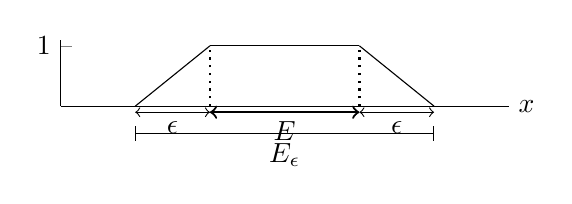
\begin{tikzpicture}
    \begin{axis}[
    axis lines*=left,
    clip = false,
    xmin = 0, xmax = 1, 
    ymin = 0, ymax = 1.1, 
    xtick = \empty, 
    ytick = {1},
    yticklabels={$1$}, 
    axis lines* = left,
    width=0.6\textwidth, height=0.2\textwidth]
    \addplot[domain=1/6:1/3] {6*(x-1/6)};
    \addplot[domain=1/3:2/3] {1};
    \addplot[domain=2/3:5/6] {6*(5/6-x)};
    \addplot[mark=none, black, thick, dotted] coordinates {(1/3,0) (1/3,1)};
    \addplot[mark=none, black, thick, dotted] coordinates {(2/3,0) (2/3,1)};
    \node [right] at (current axis.right of origin){$x$};
    \draw[<->, thick] (1/3, -0.1) to (2/3, -0.1);
    \draw[<->] (1/6, -0.1) to (1/3, -0.1);
    \draw[<->] (2/3, -0.1) to (5/6, -0.1);
    \draw[|-|] (1/6, -0.45) to (5/6, -0.45);
    \node [below] at (1/4, -0.1) {$\epsilon$};
    \node [below] at (3/4, -0.1) {$\epsilon$};
    \node [below] at (1/2, -0.1) {$E$};
    \node [below] at (1/2, -0.45) {$E_\epsilon$};
    \end{axis}
\end{tikzpicture}
\end{center}
Let $E_\epsilon := \set{x \,|\, \rho(x,E) < \epsilon}$. Then clearly 
\begin{equation*}
    \chi_E \leq g_\epsilon \leq \chi_{E_\epsilon} \implies \mu(E) \leq \int_X g_\epsilon(x) \, \mu(dx) = \int_X g_\epsilon(x) \, \nu(dx) \leq \nu(E_\epsilon).
\end{equation*}
But as $\epsilon \searrow 0$ we have $E_\epsilon \searrow E$ and hence by continuity from above we have $\nu(E_\epsilon) \searrow \nu(E)$, so $\mu(E) \leq \nu(E)$. Interchanging $\mu$ and $\nu$ completes the proof.
\end{proof}

As a corollary, 
\begin{corollary}[Uniqueness of weak limit]
If $\mu_n \to \mu$ and $\mu_n \to \nu$ weakly then $\mu = \nu$.
\end{corollary}

\begin{unexaminable}
We may relate the weak convergence of a sequence of measures to functional analysis. This discussion is optional if you have not previously studied functional analysis before, and a good reference would be chapter 3 of \cite{BrezisFuncAnalysis} or section 4.9 of \cite{KreyszigFuncAnalysis}. Recall that $C_b(X)$ is itself a \textbf{Banach} space (i.e. complete normed vector space) equipped with the supremum norm:
\begin{equation}
    \norm{f}_\infty := \norm{f}_{C_b(X)} := \sup_{x \in X} |f(x)|
\end{equation}
We may consider \textbf{functionals} $T: f \mapsto Tf$ that are linear maps from $C_b(X)$ to $\R$. A functional $T$ is bounded (equivalent to being continuous) if there is a constant $C > 0$ such that for all $x$ one have $|Tf(x)| \leq \norm{f}_{C_b(X)}$. The supremum norm now induces a norm on the \textbf{dual space} of $C_b(X)$, i.e. vector space of all bounded linear functional $C_b(X)'$, which is defined as followed:
\begin{equation}
    \norm{T}_{C_b(X)'} := \sup_{f \in C_b(X)} \frac{|Tf|}{\norm{f}_{C_b(X)}} = \inf \set{C>0 \,|\, \forall f \in C_b(X), |Tf| \leq C\norm{f}_{C_b(X)}}.
\end{equation}

\begin{exercise}
Let $\mu$ be a probability measure on $X$. Check that the map 
\begin{equation*}
    T_\mu: f \mapsto \int_X f(x) \, \mu(dx)
\end{equation*}
is a bounded linear functional on $C_b(X)$ with $\norm{T_\mu}_{C_b(X)'} = 1$.
\end{exercise}

We note that there are at least two notions of convergence of functionals in $C_b(X)$: consider functionals $T_n, T \in C_b(X)'$ with $n \in \Z_{\geq 1}$
\begin{itemize}
    \item $T_n \to T$ \textbf{uniformly} if $\norm{T_n - T}_{C_b(X)'} \to 0$ as $n \to \infty$.
    \item $T_n \to T$ \textbf{weakly*} if for all $x \in X$ we have $T_n x \to Tx$. (This corresponds to pointwise convergence).
\end{itemize}

As an important example (which is the point of going through this discussion on this functional analysis topic):
\begin{example}
$\mu_n \to \mu$ weakly $\iff$ $T_{\mu_n} \to T_\mu$ weakly*.
\end{example}

\begin{remark}
Do not be confused with the notion of weak convergence! Weak convergence usually describes the convergence of elements inside a Banach space, not its dual! Of course, one could say that $T_n \to T$ \textbf{weakly} as elements of $C_b(X)'$ as the "intended" Banach space, which refers to $gT_n \to gT$ for all $g$ in the \textbf{double dual} (dual of dual) space $C_b(X)''$. Note that this is strictly stronger than weak* convergence. This is because all evaluation maps $\mathsf{ev}_x: T \mapsto Tx$ are elements in $C_b(X)''$, which means 
\begin{equation*}
    T_n \to T \; \text{weakly} \implies \mathsf{ev}_x T_n = T_n x \to \mathsf{ev}_x T = Tx;
\end{equation*}
but not all elements in $C_b(X)''$ can be represented by the evaluation of an element in $C_b(X)$. In general, the notions of weak and weak* convergence coincide only when we are looking at Banach space for which its double dual coincides with itself.
\end{remark}

We may therefore use the tools from functional analysis to prove theorems relating to weak convergence of measures. For example, we may draw parallels from proposition 3.12 to prove that weakly* convergence induces a topology on the set of probability measures on $(X,\B(X))$, which is generated by neighbourhoods of the following form:
\begin{equation}
    U_{f_1,...,f_k,\epsilon}(\mu) := \set{\nu \,\bigg|\, \forall i = 1,...,k, \abs{\int_X f_i \, \mu(dx) - \int_X f_i \, \nu(dx)} < \epsilon}
\end{equation}
where $\mu, \nu$ is a probability measure on $X$. This also motivates the following definition of the Levy-Prokhorov metric:
\begin{equation}
    \pi(\mu,\nu) := \inf \set{\epsilon > 0 \,|\, \mu(A) \leq \nu(A_\epsilon) + \epsilon \text{ and } \nu(A) \leq \mu(A_\epsilon) + \epsilon},
\end{equation}
where $A_\epsilon := \set{x \,|\, \rho(x,A) < \epsilon}$ is as defined in the proof of lemma \ref{lem:uniqueness_by_integral}. The induced topology is also Polish, which is particularly useful when we want to talk about random probability measures.

\begin{exercise}
Show that for the case when $(X,\B(X)) = (\R,\B(\R))$ then the probability measures $\mu_n \to \mu$ weakly iff $\pi(\mu_n, \mu) \to 0$.  
\end{exercise}

\begin{hint}
Each probability measure of $(\R,\B(\R))$ can be represented by a distribution function. Rewrite the definition of the Levy-Prohorov metric to gain more insights.
\end{hint}
\end{unexaminable}

\subsection{Portmanteau Theorem and related facts}
But wait! We have defined the notion of convergence in distribution in another way in elementary probability classes. Specifically if $(X,\B(X)) = (\R, \B(\R))$ then we say $\xi_n \to \xi$ in distribution if the distribution function $F_{\xi_n}(x) \to F_{\xi}(x)$ for all $x$ when $F_\xi$ is continuous. Turns out the Portmanteau theorem provides us with the required equivalence. This theorem was given its name since it involves a lot of equivalent statements, which look like lots of coats hanging on a coat hanger (\textit{Portmanteau} in French). \footnote{Figure provided by Hobvias Sudoneighm \url{https://www.flickr.com/people/34427466731@N01} under the Creative Common 2.0 License: \url{https://creativecommons.org/licenses/by-sa/2.0/}}

\begin{theorem}[Portmanteau Theorem] \label{def:conv_in_dist}
Let $(X,\B(X))$ be a Polish space induced by a metric $d$ and $\mu_n, \mu$ are measures with $\mu_n(X), \mu(X) \leq 1$. Writing $\E_\mu$ as expectation (or integral) with respect to the probability measure $\mu$, then the following are equivalent.
\begin{enumerate}
    \item $\mu_n \to \mu$ weakly, that is, $\forall f \in C_b(X)$, $\E_{\mu_n}[f] \to \E_\mu[f]$.
    \item For all \textbf{uniformly} continuous $f \in C_b(X)$, $\E_{\mu_n}[f] \to \E_\mu[f]$.
    \item For all \textbf{bounded} $f \in \Lip(X)$, $\E_{\mu_n}[f] \to \E_\mu[f]$.
    \item For all bounded measurable $f$ with $\mu(U_f) = 0$, $\E_{\mu_n}[f] \to \E_\mu[f]$, where $U_f$ is the set when $f$ is discontinuous.
    \item $\mu_n(X) \overset{n\to\infty}{\to} \mu(X)$, and for any closed set $E \subseteq X$, $\limsup \mu_n(E) \leq \mu(E)$.
    \item $\mu_n(X) \overset{n\to\infty}{\to} \mu(X)$, and for any open set $O \subseteq X$, $\liminf \mu_n(\xi_n \in O) \ge \mu(\xi \in O)$.
    \item (Convergence in general) $\lim \mu_n (\xi_n \in C) = \mu(\xi \in C)$ for any $C$ such that $\mu(\xi \in \partial C) = 0$.
    % \item Let $F_{\xi_n}(x)$ be the distribution function of $\xi_n$ and similarly for $F_{\xi}(x)$, then $F_{\xi_n}(x) \to F_\xi (x)$ (pointwise) at any point of continuity of $F_\xi(x)$.
\end{enumerate}
\end{theorem}

\begin{center}
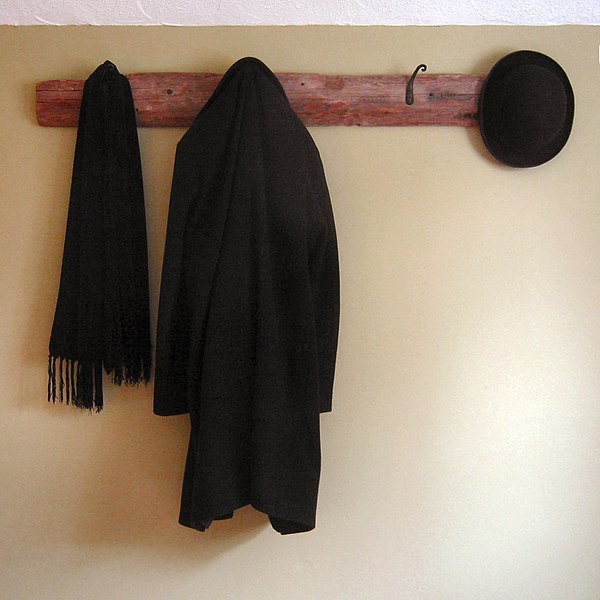
\includegraphics[width=0.5\textwidth]{figures/hanger.jpg}
\end{center}

\begin{proof} We will follow the order of proving $(4) \implies (1) \implies (2) \implies (3) \implies (5) \implies (6) \implies (7) \implies (4)$. \\

$(4) \implies (1) \implies (2) \implies (3)$. This is trivial.\\

$(3) \implies (5)$. The first condition can be proven by applying (3) with $f \equiv 1$. For the second condition, recall in the proof of lemma \ref{lem:uniqueness_by_integral} we have defined a Lipschitz approximation for any indicator functions of a closed set $E$, which is denoted as $g_\varepsilon(x)$ in equation \eqref{eq:Lipschitz_approx_indicator}. Define also $E_{\varepsilon} = \{ x : \rho(x,E) < \varepsilon\}$. Note that $E_\varepsilon \searrow E$ as $\varepsilon \searrow 0$, so we have
\begin{equation*}
    \mu_n(E) = \int f \, \d \p_n \le \int g_\epsilon \, \d \mu_n.
\end{equation*}
Therefore
\begin{align*}
    \limsup_{n \to \infty} \mu_n(E) \le \limsup_{n \to \infty} \int g_\varepsilon \, \d \mu_n \overset{(3)}{=} \int g_\varepsilon \, \d \mu \leq \mu(E_\varepsilon).
\end{align*}
Since the above inequality holds for all $\epsilon > 0$, we can send $\epsilon \to 0$ to conclude that
\begin{align*}
    \limsup_{n \to \infty} \mu_n(E) \le \mu(E)
\end{align*}
as required. \\

($5 \iff 6$). consider $O = X \backslash E$, $B$ being closed. \\

($5,6 \implies 7$). recall that $\overline{C} = C \cup \partial C$; $C^\circ := \text{int}\, C = C \backslash \partial C$. Since $\p(\xi \in \partial C) = 0$.
\begin{align*}
    &\limsup \mu_n(C) \le \limsup \mu_n (\overline{C}) \overset{(5)}{\le} \mu(\overline{C}) = \mu(C), \\
    &\liminf \mu_n(C) \ge \liminf \mu_n(C^\circ) \overset{(6)}{\ge} \mu(C^\circ) = \mu(C),
\end{align*}
so $\lim \mu_n(C) = \mu(C)$. \\

($7 \implies 4$). Let $f:X \to \R$ be a bounded and measurable function with $\mu(U_f) = 0$. We make the following claims:\\

\textbf{Claim 1:} For all $D \subseteq \R$, $\partial f^{-1}(D) \subseteq f^{-1}(\partial D) \cup U_f$.

\begin{hint}
What happen if $x \in \partial f^{-1}(D)$ but $x \notin U_f$, i.e. $f$ is continuous at $x \in E$? Recall the definition of continuity at $x \in E$: $\forall \epsilon > 0,\; \exists \delta := \delta(\epsilon) > 0$ such that $f(B_\delta(x)) \subseteq B_\epsilon(f(x))$. Also recall that $f(x) \in \partial D$ iff $\forall \epsilon > 0$, $B_\epsilon(D) \cap A \neq \varnothing$ and $B_\epsilon(D) \cap A^c \neq \varnothing$.
\end{hint}

\textit{Proof of claim 1.} Fix $\epsilon>0$ and extract $\delta := \delta(\epsilon)$ as above. Provided that $x \in \partial f^{-1}(D)$, we know that there is a $y \in B_\delta(x) \cap f^{-1}(D)$ and $z \in B_\delta(x) \cap X\setminus f^{-1}(D)$. We therefore have
\begin{align*}
    f(y) \in f(B_\delta(x) \cap f^{-1}(D)) \subseteq f(B_\delta(x)) \cap f(f^{-1}(D)) \subseteq B_\epsilon(f(x)) \cap D 
\end{align*}
and similarly $f(z) \in B_\epsilon(f(x)) \cap D^c$. Since $\epsilon > 0$ is arbitrary we have $f(x) \in \partial D$ as desired. \\

\textbf{Claim 2:} Consider the set $A := \set{y \in \R \,|\, \mu(f(x) = y) > 0}$, i.e. set of atoms of the finite push-forward measure $f^*\mu$. Then $A$ must be countable.\\

We leave that as an exercise.\\

\textit{Finishing the proof.} Fix $\epsilon > 0$ and let $\norm{f}_\infty = \sup_{x\in X} |f(x)|$ (for the case when $f$ is continuous then $\norm{f}_\infty$ coincides with $\norm{f}_{C_b(X)}$).  Then by claim 2, we may choose $N+1$ "grid points" such that 
\begin{equation*}
    y_0 \leq -\norm{f}_\infty < y_1 < ... < y_{N-1} < \norm{f}_\infty < y_N,
\end{equation*}
such that for all $i$,
\begin{equation*}
    y_i \in \R \setminus A \quad \text{and} \quad y_{i+1} - y_i < \epsilon.
\end{equation*}

Now let $X_i = f^{-1}([y_{i-1}, y_i))$ for $i=1,...,N$. Then $X = \sqcup_{i=1}^N X_i$. By claim 1, we have
\begin{equation*}
    \mu(\partial X_i) \leq \mu(f^{-1}(\set{y_{i-1}})) + \mu(f^{-1}(\set{y_{i}})) + \mu(U_f) = 0
\end{equation*}

Therefore,
\begin{align*}
    \limsup_{n\to\infty} \int f \, \mu_n(dx) \leq \limsup_{n\to\infty} \sum_{i=1}^N y_i \mu_n(E_i) \overset{(7)}{=} \sum_{i=1}^N y_i \mu(E_i) \leq \epsilon \mu(X) + \sum_{i=1}^N y_{i-1} \mu(E_i) \leq \varepsilon + \int f \, \mu(dx)
\end{align*}

Since the above arguments hold for arbitrary $\epsilon > 0$, we see that 
\begin{equation*}
\limsup_{n\to\infty} \int f \, \mu_n(dx) \leq \int f \, \mu(dx)
\end{equation*}
We complete the proof by applying the above inequality with $-f$ to obtain the reverse inequality:
\begin{equation*}
\limsup_{n\to\infty} \int -f \, \mu_n(dx) \leq \int -f \, \mu(dx) \iff \int f \, \mu(dx) \leq \liminf_{n\to\infty} \int f \, \mu_n(dx)
\end{equation*}
\end{proof}

\begin{exercise}
\begin{enumerate}
    \item[]
    \item Rewrite the statements of Portmanteau theorem for a sequence of random variables that converge in distribution.
    \item Fill in the gap: prove that there are at most countable atoms for the finite measure $f^*\mu$.
\end{enumerate}
\end{exercise}

\begin{hint}
Argue by contradiction. The key step is to convince yourself that if $A$ is uncountable then there is an $\epsilon > 0$ such that $f^*\mu((\set{x})) \geq \epsilon$ for uncountably many $x \in A$ (otherwise you will have $A$ being countable!)
\end{hint}

We now look at some applications of the Portmanteau theorem:
\subsubsection{Slutsky's Theorem and Convergence of Probability}
Slutsky's theorem is the core of establishing the fact that convergence in probability implies convergence in distribution, as well as a couple of other facts relating to the arithmetic of weak limits of converging sequence of random variables. Let us now go through the statement of Slutsky's theorem:

\begin{theorem}[Slutsky]
Consider random variables $\xi, \xi_1,...$ and $\eta,\eta_1,...$ from $(\Omega,\F,\p)$ to the Polish space $(X,\B(X))$ with metric $d$. Assume $\xi_n \overset{n\to\infty}{\to} \xi$ in distribution and $d(\xi_n, \eta_n) \overset{n\to\infty}{\to} 0$ in probability. Then $\eta_n \overset{n\to\infty}{\to} \xi$ in distribution.
\end{theorem}

\begin{proof}
Let $f:X \to \R$ be a bounded and Lipschitz function $f \in \Lip_{K}(X)$. Then for all $x \in E$,
\begin{equation}
    \abs{f(x) - f(y)} \leq Kd(x,y) \wedge 2\norm{f}_{C_b(X)}.
\end{equation}
So by dominated convergence theorem one have $\limsup_{n\to\infty} \E_{\p}[|f(\xi_n) - f(\eta_n)|] = 0$. But we also have $\limsup_{n\to\infty} \E_{\p}[|f(\xi_n) - f(\xi)|] = 0$ by convergence in probability, so combining yields $\limsup_{n\to\infty} \E_{\p}[|f(\eta_n) - f(\xi)|] = 0$. By statement (3) of the Portmanteau theorem we have $\eta_n \overset{n\to\infty}{\to} \xi$ in distribution.
\end{proof}

As an immediate corollary:
\begin{corollary} \label{cor:prob_implies_dist}
Let $\xi_n, \xi: (\Omega,\F,\p) \to (X,\B(X))$, then $\xi_n \overset{n\to\infty}{\to} \xi$ in probability implies $\xi_n \overset{n\to\infty}{\to} \xi$ in distribution. Moreover if $\xi_n \overset{d}{\to} \xi$ and $\xi \equiv c$ for some constant $c$, then $\xi_n \overset{p}{\to} c$.
\begin{figure} [H]
    \centering
    \begin{tikzcd}
    & \overset{L^p}{\to} \arrow[Rightarrow, d]  & \\
    \overset{a.e.}{\to} \arrow[Rightarrow, r] & \textcolor{red}{\overset{p}{\to}} \arrow[Rightarrow, r, red] & \textcolor{red}{\overset{d}{\to}}
\end{tikzcd}
\end{figure}
\end{corollary}

\begin{proof} 
First statement is proven by applying $\xi_n \equiv \xi$. As for the second statement, let's say $\xi_n \overset{d}{\to} c$ where $c$ is a constant. Then by utilising statement (5) of the Portmanteau theorem, we know that
\begin{equation*}
    \lim_{n\to \infty} \p(d(\xi_n, c) \geq \epsilon) = \lim_{n\to \infty} \p(\xi_n \in X \setminus B_\epsilon(c)) \leq \p(c \in X \setminus B_\epsilon(c)) = 0.
\end{equation*}
\end{proof}

\begin{remark}
\begin{itemize}
\item[]
\item An alternative proof of the partial converse is as followed: if we assume the metric form of convergence in probability, then we can directly write 
\begin{equation}
    \E[d(X_n, c) \wedge 1] \overset{n\to\infty}{\to} 0,
\end{equation}
noticing that the function $f(.) = d(.,c) \wedge 1$ is a continuous and bounded function on $X$.
\item A counter-example showing convergence in distribution does not imply convergence in probability is as followed: consider a real-valued random variable $X$ that is symmetric about zero, e.g. $\xi \sim \mathsf{N}(0,1)$. Then the sequence $\xi_n := (-1)^{n+1}\xi$ converges in distribution (since they are identically distributed) but not in probability.
\end{itemize}
\end{remark}

Here is an example of using the above implication. 
\begin{example}[Motivation of Weierstrass Approximation Theorem]
Recall the Bernoulli's law of large numbers, that for all $p \in [0,1]$,
\begin{equation*}
    \frac{S_n}{n} \xrightarrow{p} p, \quad n \to \infty,
\end{equation*}
where $S_n = \xi_1 + \xi_2 + \cdots + \xi_n$ and $\xi_i \sim \mathsf{B}(1,p)$. Putting
\begin{equation*}
    F_n(x) = \p \bigg(\frac{S_n}{n} \le p \bigg), \quad F(x) = 
    \begin{cases}
    1, & x \ge p,\\
    0, & x<p,
    \end{cases}
\end{equation*}
where $F(x)$ is the distribution function of the constant random variable $\xi \equiv p$. Also let $\p_n$ and $\p$ be the probability measures on $(\R, \B(\R))$ corresponding to the distributions $F_n, F$. The above implication implies that $S_n/n \xrightarrow{d} p$, which means from statement (1) that
\begin{equation*}
    \E\bigg[f\bigg(\frac{S_n}{n} \bigg) \bigg] \to \E[f(p)] = f(p), \quad n \to \infty,
\end{equation*}
for every bounded function $f(x) \in C_b(\R)$. Since $S_n \sim \mathsf{B}(n,p)$, we know that
\begin{equation*}
    \E\bigg[f\bigg(\frac{S_n}{n} \bigg) \bigg] = \int_\R f(x) \, \p_n(\d x) = \sum_{k=0}^n \sqbracket{{n \choose k}(1-p)^{n-k} p^k} f\bracket{\frac{k}{n}} =: f_n(p)
\end{equation*}
which is a polynomial in $p$. We therefore have for all $f \in C_b(\R)$, $f_n(p) \to f(p)$ pointwise for all $p \in [0,1]$. Restricting $f$ to the compact interval $[0,1]$, we have recovered a weakened version of the Weierstrass approximation theorem, that there is a sequence of polynomials $f_n$ such that $f_n \to f$ pointwise on $[0,1]$. The actual approximation theorem goes further and establishes that the above convergence is actually uniform on $[0,1]$.
\end{example}

Here is another application of Slutsky's theorem regarding the addition of weak limits. This result is also named after Slutsky due to its relation with the original Slutsky's theorem.
\begin{proposition}[Slutsky, Addition of Limits] \label{prop:addition_of_weak_limits}
Consider random variables $\xi, \xi_1,...$ and $\eta_1,...$ from $(\Omega,\F,\p)$ to $(\R,\B(\R))$ (or any Polish space with addition defined). Assume $\xi_n \overset{n\to\infty}{\to} \xi$ in distribution and $\eta_n \overset{n\to\infty}{\to} c$ in probability, with $c$ being a constant. Then $\xi_n + \eta_n \overset{n\to\infty}{\to} \xi + c$ in distribution.
\end{proposition}

\begin{proof}
First it is easily to check by that $\xi_n + c \overset{n\to\infty}{\to} \xi_n + c$ in distribution. (This can be done by e.g. shifting the closed sets and applying statement (5) of the Portmanteau theorem. Now note that $|(\xi_n + \eta_n) - (\xi_n + c)| \overset{n\to\infty}\to 0$ in probability, so by Slutsky's theorem we have $\xi_n + \eta_n \to \xi_n + c$ in distribution.
\end{proof}

Note that it is not true in general that both $\xi_n \overset{n\to\infty}\to \xi$ and $\eta_n \overset{n\to\infty}\to \eta$ in distribution implies $\xi_n + \eta_n \overset{n\to\infty}\to \xi + \eta$ in distribution. As an example, consider again the real-valued random variable $\xi$ that is symmetric about zero. If $\xi_n \equiv \xi$ and $\eta_n = (-1)^{n+1} \xi$, then $\xi_n + \eta_n$ takes the form $(2\xi, 0, 2\xi, 0, ...)$ which does not converge in distribution.\\

Traditionally, Slutsky's theorem also contains the following statements
\begin{proposition}[Slutsky, Multiplication/Division of Limits] \label{prop:mult_of_weak_limits}
Under the same setting as proposition \ref{prop:addition_of_weak_limits}, we have $\xi_n \eta_n \overset{n\to\infty}{\to} c\xi$ in distribution. In addition if $c \neq 0$ then $\xi_n / \eta_n \overset{n\to\infty}{\to} \xi / c$.
\end{proposition}

To prove this, we note the following result:
\begin{proposition}[Continuous Mapping Theorem] 
Let $(X_1,\B(X_1))$ and $(X_2,\B(X_2))$ be metric spaces generated by metric $d_1$ and $d_2$ respectively, and let $\varphi: X_1 \to X_2$ be measurable. If $U_\varphi$ is the set of points of discontinuity of $\varphi$ (which is Borel measurable), then
\begin{enumerate}
\item If $\mu, \mu_1, \mu_2, ...$ are measures on $(X_1,\B(X_1))$ with $\mu(X_1), \mu_n(X_1) \leq 1$ and $\mu(U_\varphi) = 0$ and $\mu_n \overset{n\to\infty}\to \mu$ weakly, then $\varphi^*\mu_n \overset{n\to\infty}{\to} \varphi^*\mu$ weakly.
\item If $\xi, \xi_1, \xi_2, ...: (\Omega,\F,\p) \to (X_1, \B(X_1))$ are random variables with $\p(\xi \in U_\varphi) = 0$ and $\xi_n \overset{n\to\infty}\to \xi$ in distribution, then $\varphi(\xi_n) \overset{n\to\infty}\to \varphi(\xi)$
\end{enumerate}
\end{proposition}

\begin{proof}
Note that the second statement is an immediate result of the first one. To prove the first statement, we are required to show that for all $f \in C_b(X_2)$,
\begin{align*}
    \lim_{n\to\infty} \int_{X_2} f(x_2) \,\varphi^*\mu_n(dx_2) &\overset{\text{(LOTUS)}}{=} \lim_{n\to\infty} \int_{X_1} f(\varphi(x_1)) \,\mu_n(dx_1) \\
    &\overset{(*)}{=} \int_{X_1} f(\varphi(x_1)) \,\mu(dx_1) \\
    &\overset{\text{(LOTUS)}}{=} \int_{X_2} f(x_2) \, \varphi^*\mu(dx_1).
\end{align*}
The first and third equality is justified by the use of the change of variable formula (theorem \ref{thm:LOTUS}). The second equality is justified by noting that $U_{f \circ \varphi} \subseteq U_\varphi$, so $\mu(U_{f \circ \varphi}) = 0$ and we may use statement (4) of the Portmanteau theorem to conclude.
\end{proof}

We also note the following:
\begin{exercise}
Under the setting of proposition \ref{prop:addition_of_weak_limits}, consider the random variables $T_n: \omega \in \Omega \mapsto (\xi_n(\omega), \eta_n(\omega))$ and $T: \omega \in \Omega \mapsto (\xi_n(\omega), c)$. Then $T, T_n$ are $(\R^2, \B(\R^2))$-valued random variables. Show that $T_n \overset{n\to\infty}\to T$ in distribution. 
\end{exercise}

\begin{hint}
Try mimick the proof of proposition \ref{prop:addition_of_weak_limits} by proving that $(X_n, c) \overset{n\to\infty}{\to} (X_n, c)$ in distribution and $|(X_n, Y_n) - (X_n, c)| \overset{n\to\infty}{\to} 0$ in probability, then utilise Slutsky's theorem.
\end{hint}

\begin{proof}
\textit{of proposition \ref{prop:addition_of_weak_limits}/\ref{prop:mult_of_weak_limits}.} Apply the result in the above exercise and continuous mapping theorem with map $\varphi(x,y) = x+y$, $xy$ or $x/y$.
\end{proof}

\subsubsection{Convergence of distribution function}
Let us finally connect our definition of weak convergence with the definition of convergence of distribution in elementary probability classes, that is, the convergence of the distribution function. We restrict our discussion to real-valued random variables, although it can be extended to random variables taking value on $\R^n$.

\begin{theorem}[Convergence in distribution] \label{thm:conv_in_dist_func}
\begin{enumerate}
\item[]
\item Consider measures $\mu, \mu_n$ on $(\R,\B(\R))$ with $\mu(\R), \mu_n(\R) \leq 1$ and define their distribution functions $F(x) := \mu((-\infty,x])$ and $F_n(x) := \mu_n((-\infty, x])$. Then $\mu_n \overset{n\to\infty}{\to} \mu$ weakly $\iff$ 
\begin{itemize}
\item $F_n(x) \overset{n\to\infty}\to F(x)$ for all $x \in \R \setminus U_F$, $U_F$ being the set of discontinuities of $F$, and 
\item $F_n(+\infty) \to F(+\infty) =: \lim_{x\to +\infty} F(x)$. 
\end{itemize}

\item Consider random variables $\xi_n, \xi : (\Omega,\F,\p) \to (\R,\B(\R))$, then $\xi_n \overset{n\to\infty}{\to} \xi$ in distribution $\iff$ 
\begin{itemize}
\item $F_{\xi_n}(x) \overset{n\to\infty}{\to} F_\xi(x)$ when $x \in \R \setminus U_{F_\xi}$.
\item $F_{\xi_n}(+\infty) \overset{n\to\infty}{\to} F_\xi(+\infty)$
\end{itemize}
\end{enumerate}
\end{theorem}

\begin{remark} \label{rmk:weakening_conv_in_dist}
We note that convergence at all points of continuity implies 
\begin{equation}
F(+\infty) \leq \liminf_{n\to\infty} F_{n}(+\infty)
\end{equation}
To see this, we note that for all $x$, we have $F(x) \leq \liminf_{n\to\infty} F_n(+\infty)$. Fix an $x \in \R$, then there is an $r > x$ such that $F$ is continuous at $r$. At this point we have $\liminf_{n\to\infty} F_n(r) = \lim_{n\to\infty} F_n(r) = F(r)$. Now note that, for all $n$, $F_n(r) \leq F_n(+\infty)$, so we have $F(x) \leq \liminf_{n\to\infty} F_{n}(+\infty)$. Since $x$ is arbitrary, we know that $F(+\infty) \leq \liminf_{n\to\infty} F_{n}(+\infty)$.\\

From this, we know that if $F(+\infty) \geq \limsup_{n\to\infty} F_n(+\infty)$, then $\mu_n \overset{n\to\infty}{\to} \mu$ weakly.
\end{remark}

\begin{proof}
We note that statement (2) immediately follows from (1). For the $(\Rightarrow)$ direction, it follows from the fact that $\mu(\partial (-\infty, x]) = \mu(\set{x}) = 0$ whenever $F$ is continuous at $x$, so by statement (7) of Portmanteau theorem we have $F_n(x) \overset{n\to\infty}{\to} F(x)$. For the $(\Leftarrow)$ direction, we attempt to use statement (3) of the Portmanteau theorem; that is, if $f$ is a bounded Lipschitz function (wlog $f \in \Lip_1(\R)$ and bounded by $1$), then
\begin{equation*}
    \lim_{n\to\infty} \int_\R f(x) \, \mu_n(dx) = \int_\R f(x) \, \mu(dx).
\end{equation*}
Using arguments in proving $(7) \implies (4)$ in the Portmanteau theorem, we know that $U_F$ is countable. As a result, we may choose $N$ "knot points", but in a way different from the one in the proof of the Portmanteau theorem. Specifically, we want
\begin{equation*}
    y_1 < y_2 < ... < y_{N-1}
\end{equation*}
such that for all $i$,
\begin{equation*}
    y_i \notin U_F, \quad y_i - y_{i-1} < \epsilon, \quad F(y_1) < \epsilon, \quad F(y_{N-1}) > F(\infty) - \epsilon.
\end{equation*}
With the notation of $y_0 = -\infty$ and $y_N = \infty$ (so that $F(y_0)=F_n(y_0)=0$), we obtain the bound:
\begin{align*}
    \int f(x) \, \mu_n(dx) = \sum_{i=0}^n f(x) \, \mu_n(dx) &\leq F_n(y_1) + F_n(\infty) - F_n(y_{N-1}) + \sum_{i=1}^{N-1} \int_{y_i}^{y_{i+1}} f(x) \, \mu_n(dx).
\end{align*}
But we know that for all $x \in [y_i, y_{i+1})$ 
\begin{equation*}
    |f(x) - f(y_i)| \leq |x-y_i| \leq y_i - y_{i-1} < \epsilon \implies f(y_i) - \epsilon < f(x) < f(y_i) + \epsilon,
\end{equation*}
so
\begin{align*}
    \int f(x) \, \mu_n(dx) &< \bracket{F_n(y_1) + F_n(\infty) - F_n(y_{N-1})} + \sum_{i=1}^{N-1} (f(y_i) + \epsilon)(F_n(y_{i+1}) - F_n(y_{i})) \\
    &= \bracket{F_n(y_1) + F_n(\infty) - F_n(y_{N-1})} + \sum_{i=1}^{N-1} f(y_i)(F_n(y_{i+1}) - F_n(y_{i})) + \epsilon F_n(\infty)
\end{align*}
Note that for all $i$, $F_n(y_i) \overset{n\to\infty}{\to} F(y_i)$. Recall that $F(\infty) \leq 1$, we have
\begin{align*}
    \limsup_{n\to\infty} \int f(x) \, \mu_n(dx) &< 3\epsilon + \sum_{i=1}^{N-1} f(y_i)(F(y_{i+1}) - F(y_{i})) \\
    &\leq \int_{i=1}^{N-1} \int_{y_i}^{y_{i+1}} (f(x)+\epsilon) \, \mu(dx) \\
    &\leq 4\epsilon + \int f(x) \, \mu(dx)
\end{align*}
owing to the fact that $f(x) + \epsilon \geq f(y_i)$ for all $x \in [y_i, y_{i+1})$. Sending $\epsilon \searrow 0$ yields
\begin{align*}
    \limsup_{n\to\infty} \int f(x) \, \mu_n(dx) \leq \int f(x) \, \mu(dx)
\end{align*}
Replacing $f$ by $(1-f)$ yields the desired reverse inequality.
\end{proof}

Here we raise some applications of the above result. First of all, (theorem \ref{thm:deMoivre_CLT})
\begin{example}[de Moivre's Central Limit Theorem] \label{ex:deMoivre_CLT_conv_dist}
For $\xi_i \overset{\mathsf{iid}}{\sim} \mathsf{B}(1,p)$ and $S_n = \sum_{i=1}^n \xi_i$, recall the random variable $\eta_n = (S_n-np)/\sqrt{np(1-p)}$ satisfies
\begin{equation*}
    \lim_{n \rightarrow \infty} \p (\eta_n \le x) = \Phi (x),
\end{equation*}
where $\Phi(x)$ is the distribution function of the standard normal $\mathsf{N}(0,1)$ distribution. Therefore, \textbf{the probability distribution of $\eta_n$ converges to a $\mathsf{N}(0,1)$ distribution}. By definition of weak convergence, for any $f \in C_b(\R)$ we know that
\begin{equation}
\E\sqbracket{f\bracket{\frac{S_n-np}{\sqrt{np(1-p)}}}} \overset{n\to\infty}{\to} \int_\R f(t) \bracket{\frac{1}{\sqrt{2\pi}} e^{-t^2/2}} \, dt
\end{equation}
\end{example}

Here is another shortcut for proving convergence in distribution via the convergence of their densities.

\begin{corollary}
Suppose that the random variables $\xi_n, \xi$ have densities $f_n(x), f(x)$, respectively. Also let $f_n(x) \to f(x)$ for any $x$. Then $\xi_n \xrightarrow{d} \xi$.
\end{corollary}

\begin{proof}
It is sufficient to show that 
\begin{equation*}
    F_n(x) = \int_{-\infty}^x f_n(y) \, \d y \to F(x) = \int_{-\infty}^x f(y) \, \d y
\end{equation*}
for any $x$. Using 
\begin{equation*}
    |F_n(x) - F(x)| \le \int_{-\infty}^x |f_n(y) - f(y)| \, \d y,
\end{equation*}
we need to check that
\begin{equation*}
    \lim_{n \to \infty} \int_{-\infty}^\infty |f_n(y) - f(y)| \, \d y = 0.
\end{equation*}
Note that $a = a_+ - a_-$ and $|a| = a_+ + a_-$ for any real $a$. Since $f_n$ and $f$ are densities, they integrate to $1$, so for each $n$
\begin{equation*}
    0 = \int_{-\infty}^\infty (f(y) - f_n(y)) \, \d y = \int_{-\infty}^\infty [(f(y) - f_n(y))_+ - (f(y) - f_n(y))_-] \, \d y.
\end{equation*}
Then
\begin{equation*}
    \int_{-\infty}^\infty |f(y) - f_n(y)| \, \d y = 2\int_{\infty}^\infty(f(y) - f_n(y))_+ \, \d y,
\end{equation*}
which goes to zero by the dominated convergence theorem. Indeed 
\begin{equation*}
    0 \le (f(y) - f_n(y))_+ \le f(y),
\end{equation*}
for any $n$ and the function $f(y)$ is integrable.
\end{proof}

\begin{exercise}
\begin{enumerate}
    \item[]
    \item Let $F_n \to F$ and suppose that $F$ is continuous. Show that $F_n$ converges \textit{uniformly} to $F$, i.e.
    \begin{equation*}
        \sup_x |F_n(x) - F(x)| \to 0, \quad n \to \infty.
    \end{equation*}
    \textit{Hint:} Idea is to consider knot points as in theorem \ref{thm:conv_in_dist_func}.
    \item Give an example of distribution functions $F_n(x), F(x)$ such that $F_n(x) \xrightarrow{d} F(x)$, but 
    \begin{equation*}
        \sup_x |F_n(x) - F(x)| \not \to 0, \quad n \to \infty.
    \end{equation*}
    \item Give an example of probability measures $\p, \p_n$ on $(\R, \B(\R))$, $n \ge 1$ such that $\p_n \xrightarrow{d} \p$, but convergence $\p_n(B) \to \p(B)$ need not hold for all Borel sets $B \in \B(\R)$.
\end{enumerate}
\end{exercise}

\subsection{Skorohod Representation Theorem}
We now prove that a sequence of weakly convergence probability measures can be represented as random variables defined on a common probability space.

\begin{theorem}[Skorohod Representation Theorem]
Suppose $\mu, \mu_n \, (n=1,2,...)$ are probability measures on a Polish space $(X,\B(X))$ induced by a metric $d$, so that $\mu_n \overset{n\to \infty}{\to} \mu$ weakly. Then there exists a single probability space $(\Omega', \F', \p')$ and random variables $\xi_1, \xi_2, \dots$ on it such that $\xi$ has distribution $\mu$ ($\xi^*\p = \mu$), $\xi_n$ has distribution $\mu_n$ ($\xi_n^*\p = \mu_n$) and that $\xi_n \to \xi$ $\p$-almost surely.
\end{theorem}

We will not go through the proof for general Polish space, if interested one can read Dudley's paper \cite{DudleySkorohod}. However if we limit ourselves to the case when $(X,\B(X)) = (\R, \B(\R)))$ then there is a simple proof.

\begin{proof}
Let $(\Omega',\F',\p') = ([0,1], \B([0,1], \Leb))$. Note that the probability measures $\mu, \mu_n$ induces distribution functions $F_n, F: \R \to [0,1]$. Let $F^{-1}, F_n^{-1}$ be their right inverses as defined in equation \ref{eq:right_inverse}, then by probability integral transform (proposition \ref{prop:prob_transform}), they have same distribution as $\mu$ and $\mu_n$'s respectively. It remains to prove that $F_n^{-1}(u) \to F^{-1}(u)$ almost surely as $n \to \infty$. In fact we can prove the required limit for any $u$ such that the preimage of $\set{u}$ under $F$ is finite (i.e. a singleton or empty set). Since there are only countably many $u$ such that the above condition doesn't hold (given that $F$ is increasing and right continuous), establishing the above limit will complete the proof. \\

Let $u$ be a point such that the preimage of $\set{u}$ under $F$ is finite. We make two observations:
\begin{itemize}
\item If $x < F^{-1}(u)$, then using the argument in the proof of proposition \ref{prop:prob_transform} we have $F(x) < u$. If $F$ is continuous at $x$, then by extending the arguments in the above proof of Portmanteau theorem we see that $F_n(x) \to F_\xi(x)$ as $n \to \infty$, and that for sufficiently large $n$ we have $F_n(x) < u \iff x \leq F_n^{-1}(u)$. We therefore have $x \leq \liminf_{n\to\infty} F_n^{-1}(u)$. Now consider a sequence $x_k \nearrow F^{-1}(u)$ such that $F$ is continuous as $x_k$, which exists by the fact that $F$ is increasing (otherwise $F$ have uncountable discontinuities!) Then for all $k$ one have $x_k \leq \liminf_{n\to\infty} F_n^{-1}(u)$, and that $F^{-1}(u) \leq \liminf_{n\to\infty} F_n^{-1}(u)$ by sending $k \to \infty$.
\item If $x > F^{-1}(u)$, then $F(x) \geq u$. In fact we must have $F(x) > u$, for if $F(x) = u$ then $F(y) = u$ for any $y \in [F^{-1}(u), x]$, contradicting the assumption that the preimage of singleton $\set{u}$ is finite. Repeating the above arguments yields $F^{-1}(u) \geq \limsup_{n\to\infty} F_n^{-1}(u)$.
\end{itemize}
Combining the observations we have $F_n^{-1}(u) \to F^{-1}(u)$ as desired.
\end{proof}

As a result, we may restate any theorems (including Central Limit Theorem) in terms of random variables.
\begin{example}[Restating de Moivre's CLT]
We may construct a probability space $(\Omega, \F, \p)$, random variables $\eta_n, \eta$ such that $\eta$ is normally distributed and $\sqrt{np(1-p)}\eta_n + np$ has a $\mathsf{B}(n,p)$ distribution. 
\end{example}

Of course, more effort is needed to actually construct a probability space $(\Omega, \F, \p)$, random variables $\xi_n \overset{\text{iid}}\sim \mathsf{B}(1,p)$ and $\eta \sim \mathsf{N}(0,1)$ such that the de Moivre's CLT holds, and this will be omitted in our discussion. Nevertheless, this representation theorem gives us a shortcut for proving results relating to the weak convergence.

\begin{example}[Alternative proof of the theorem \ref{thm:conv_in_dist_func}]
Let's say we have probability measures $\p_n, \p$ on $(\R,\B(\R))$ such that their distribution function converges at all points of continuity. By Skorohod representation theorem, we may construct a sequence of random variables $\bar{\xi}, \bar{\xi}_1, \bar{\xi}_2,...$ on the common probability space $([0,1], \B([0,1]), \Leb)$ with distributions $F_\xi, F_{\xi_1}, F_{\xi_2}, ...$. Let $f \in C_b(\R)$, then by change of variable and dominated (or bounded) convergence theorem, 
\begin{equation*}
    \lim \E_{\p_n} [f_n(\xi_n)] = \lim \E_{\Leb} [f_n(\bar{\xi}_n)] \overset{\text{(DCT)}}{=} \E_{\Leb}[f(\bar{\xi})] = \E_{\p}[f(\xi)],
\end{equation*}
noting that $f_n(\bar{\xi}_n) \to f_n(\bar{\xi})$ almost surely (convince yourself!) This completes the proof.
\end{example}

\subsection{Relative Compactness and Tightness}
We will later prove the well-known Central Limit Theorem by looking at characteristic functions. To establish the relationship between characteristic functions and measures, we need some tools relating to the collections of measures, including clarifying the meaning of how a collection is \textit{relatively compact} and \textit{tight}. These concepts are also very useful in proving results relating to stochastic processes and ergodic theory. We begin by the following definition:

\begin{definition}
A family of probability measures $\mathcal{P} = \{ \p_\alpha, \alpha \in A\}$ on a Polish space (and the corresponding set of distribution functions $F_\alpha$ if the underlying Polish space is $(\R^n, \B(\R^n))$) is called \textbf{relatively compact} if every sequence of measures from $\mathcal{P}$ contains a subsequence that weakly converges to a probability measure.
\end{definition}

\begin{remark}
We emphasise that in this definition the limit measure is to be a probability measure, although it need not belong to the original class $\mathcal{P}$. (This is why the word “relatively” appears in the definition.) In fact, $\mathcal{P}$ is relatively compact if its closure with respect to the Levi-Prokhorov metric is compact.
\end{remark}

As an example, the collection containing a weakly convergent sequence of measures is relatively compact. In fact, we have the following.
\begin{lemma} \label{lem:weak_conv_further_subsequence}
If $\{\p_{n}\}$ and $\p$ are probability measures, then $\p_n \xrightarrow{d} \p$ if and only if every subsequence $\{\p_{n'}\}$ of $\{\p_{n}\}$ contains a subsequence $\{\p_{n''}\}$ such that $\p_{n''} \xrightarrow{d}\p$.
\end{lemma}
\begin{proof}
From the definition of weak convergence we know that $\p_n \xrightarrow{d}\p$ if and only if the following sequence of numbers converges for any continuous bounded function $f$:
\begin{equation*}
    \int f(x) \, \p_n(\d x) \to \int f(x) \, \p (\d x).
\end{equation*}
So necessity is trivial, just take $\{n''\}=\{n'\}$. For the sufficiency, assume the converse to get a contradiction. Then there exists an $f$, an $\varepsilon>0$ and a subsequence $\{n'\}$ such that 
\begin{equation*}
    \bigg|\int f(x) \p_{n'}(\d x) - \int f \, \p(\d x) \bigg| > \varepsilon \quad \forall n'.
\end{equation*}
This clearly can not be true as by the assumption, $\p_{n''} \xrightarrow{d} \p$, so 
\begin{equation*}
    \bigg|\int f(x) \p_{n'}(\d x) - \int f \, \p (\d x) \bigg| < \varepsilon
\end{equation*}
for large enough $n''$.
\end{proof}

A given family of probability measures $\mathcal{P}$ is not necessarily relatively compact. This is illustrated by the following examples.
\begin{example} \label{ex:limits_not_a_distribution}
Let $\xi_n$ be real-valued random variables and $F_{\xi_n}(x) \to F(x)$ for all $x \in U_F$. Then $F(x)$ is not necessarily a distribution function!
\begin{enumerate}
    \item Let $\xi_n$ be $U[n, n+1]$. Then $F(x) \equiv 0$ (called runaway to infinity).
    \item Let $\xi_n$ be $U[-n, n]$. Then $F(x) \equiv 1/2$ (called spread to infinity).
\end{enumerate}
\end{example}

The following theorem will provide a necessary and sufficient condition for a family of probability measures (or finite measures) to be relatively compact. We first define the notion of tightness:
\begin{definition}[Tightness] \label{def:tightness}
A family of probability measures $\mathcal{P} = \{ \p_\alpha\}_{\alpha \in A}$ on a Polish space $(X, \B(X))$ induced by metric $d$ (or family of finite measures $\set{\mu_\alpha}_{\alpha \in A}$ with $\mu_\alpha(X) \leq 1$) is \textbf{tight} if for all $\varepsilon>0$ there exists a compact set $K \subset X$ such that
\begin{equation}
    \sup_{\alpha \in A} \p_\alpha (X \backslash K) \le \varepsilon.
\end{equation}
\end{definition}

Turns out tightness is a sufficient condition for relative compactness (and is necessary if $(X,\B(X))$ is Polish)
\begin{theorem}[Prokhorov's theorem]
A tight family of probability measures $\mathcal{P}$ (or finite measures as specified in definition \ref{def:tightness}) of $(X,\B(X))$ induced by metric is relatively compact. If in addition $(X,\B(X))$ is Polish then the converse also holds.
\end{theorem}

Here we only discuss the proof for the case when $(X,\B(X)) = (\R,\B(\R))$. In such case, the Prokhorov's theorem reduces to the Helly's selection theorem. We denote the collection of functions $\mathcal{G} = \{ F: \R \to [0,1] \}$ such that $F$ is nondecreasing, continuous from the right. This is called the set of generalised distribution functions. 

\begin{remark}
Distribution functions form a subset of $\mathcal{G}$ for which $F(-\infty) = 0$ and $F(\infty) = 1$.
\end{remark}

We may then state the Helly's theorem
\begin{theorem}[Helly's Selection Theorem] \label{thm:Helly_selection}
The set $\mathcal{G}$ of generalised distribution functions is sequentially compact, i.e. for any sequence $F_n \in \mathcal{G},$ $n=1,2,\dots$ there exists a function $F \in \mathcal{G}$ and a subsequence $F_{n_k} \subseteq \{ F_n\}$ such that $F_{n_k}(x) \to F(x)$ for every point $x \in \R \setminus U_F$, $U_F$ being set of points of discontinuities of $F$.
\end{theorem}

\begin{proof}
The theorem uses a classic diagonal sequence argument. Let $(q_k)_{k\geq 1}$ be an enumeration of $\Q$ (bijection from $\N$ to $\Z$). 
\begin{itemize}
\item Consider the sequence $(F_n(q_1))_{n\geq 1}$, which is bounded, so by Bolzano-Weierstrass theorem (BW) it has a subsequence $\bracket{F_{n_k^{(1)}}(q_1)}_{k \geq 1}$ which converges to some number $G(q_1) \in [0,1]$. 
\item Now consider the sequence $\bracket{F_{n_k^{(1)}}(q_2)}_{k\geq 1}$, which is also bounded, so by BW again it has a subsequence $\bracket{F_{n_k^{(2)}}(q_2)}_{k \geq 1}$ which converges to some number $G(q_2) \in [0,1]$.
\item We repeat to extract further subsequences...
\end{itemize}
We can illustrate the above procedure by picture:
\begin{equation*}
\begin{array}{cccccccccccccc}
F_1 & \boxed{F_2} & F_3 & F_4 & F_5 & F_6 & \boxed{F_7} & F_8 & F_9 & F_{10} & F_{11} & \boxed{F_{12}} & F_{13} & ... \\
 & \downarrow & & \downarrow &  & \downarrow & \downarrow & & \downarrow & \downarrow & & \downarrow & & \\
 & \boxed{F_{n^{(1)}_1}} & & F_{n^{(1)}_2} & & F_{n^{(1)}_3} & \boxed{F_{n^{(1)}_4}} & & F_{n^{(1)}_5} & F_{n^{(1)}_6} & & \boxed{F_{n^{(1)}_7}} & & ... \\
 & & & \downarrow & & & \downarrow & & \downarrow & \downarrow & & \downarrow & & \\
 & & & F_{n^{(2)}_1} & & & \boxed{F_{n^{(2)}_2}} & & F_{n^{(2)}_3} & F_{n^{(2)}_4} & & \boxed{F_{n^{(2)}_5}} & & ... \\
 & & & \downarrow & & & & & \downarrow & & & \downarrow & & \\
 & & & F_{n^{(3)}_1} & & & & & F_{n^{(3)}_2} & & & \boxed{F_{n^{(3)}_3}} & & ... \\
 & & & & & & & & \downarrow & & & \downarrow & & \\
 & & & & & & & & ... & & & ... & & 
\end{array}
\end{equation*}
We then extract the "diagonal subsequence" is as highlighted above, and write it as $F_{n_k} := F_{n_k^{(k)}}$. An important observation is that the sequence $(F_{n_k})_{k \geq \textcolor{red}{m}}$ is a subsequence of $\bracket{F_{n^{(m)}_k}}_{k\geq 1}$ for any $m \geq 1$. \\

\textbf{Claim 1:} For all $q \in \Q$, we have $F_{n_k}(q) \to G(q)$.\\

\textit{Proof of claim 1:} First find $m$ such that $q_m = q$, then note that $\bracket{F_{n_k}(q)}_{k\geq m}$ is a subsequence of $\bracket{F_{n_k^{(m)}}(q)}_{k\geq 1}$ which converges to $G(q)$. \\

\textbf{Claim 2:} $G$ is a non-decreasing function, that is if $p, q \in \Q$ and $p \leq q$, then $G(p) \leq G(q)$. This trivially follows from the monotonicity of limits.\\

As a result, we may "fill in the gaps" and define 
\begin{equation}
    F(x) = \inf \set{f(q) \,:\, q \in \Q, q > x} = \lim_{q \to x+} G(q)
\end{equation}
Then it is quite trivial that $F \in \G$. Moreover, $\forall q \in \Q$ we have $F(q) \geq G(q)$, if $x < q$ then $F(x) \leq G(q)$, and $F(q) = G(q)$. It remains to show that $F_{n_k}(x) \to F(x)$ for all $x \in \R \setminus U_F$, so let us fix $x \in \R \setminus U_F$ and some arbitrary $\epsilon > 0$. By continuity one can choose $y < r < x < q$ with $r,q \in \Q$, such that
\begin{equation*}
F(x) - \epsilon < F(y) \leq F(r) = G(r) \leq F(x) \leq F(q) = G(q) < F(x) + \epsilon,
\end{equation*}
and so for sufficiently large $k$ we have
\begin{equation*}
F_{n_k}(r), F_{n_k}(q) \in (F(x)-\epsilon, F(x)+\varepsilon) \implies F_{n_k}(x) \in (F(x)-\epsilon, F(x)+\varepsilon).
\end{equation*}
Since $\varepsilon > 0$ is arbitrary, the above arguments complete the proof.
\end{proof}

We may then prove the Prokhorov's theorem for the case when $(X,\B(X)) = (\R,\B(\R))$.
\begin{proof}
\textit{of Prokhorov's theorem for $(\R,\B(\R))$.} We first prove the partial converse. Let's say that $\mathcal{P} := \set{\mu_\alpha}_{\alpha \in A}$ is a relatively compact but not tight family of measures with $\mu_\alpha(\R) \leq 1$. Then $\exists \epsilon > 0$ such that for any compact $K \subset \R$, $\sup_\alpha \mu_\alpha(\R \setminus K) < \epsilon$. Hence, for any $n$ there is a $\mu_{\alpha_n}$ such that
\begin{equation}
\mu_{\alpha_n}(\R\setminus (-n,n)) > \epsilon. \label{eq:not_tight}
\end{equation}
By relative compactness, there is a subsequence $(\mu_{\alpha_{n_k}})_{k\geq 1}$ such that $\mu_{\alpha_{n_k}} \overset{k\to\infty}{\to} Q$ weakly, where $Q$ is a finite measure with $Q(\R) \leq 1$. By statement (5) of the Portmanteau theorem, we have
\begin{equation}
\limsup_{k\to\infty} \mu_{\alpha_{n_k}}(\R\setminus (-n,n)) \leq Q(\R \setminus (-n,n))
\end{equation}
But the RHS $\searrow 0$ as $n \to \infty$, which contradicts with \eqref{eq:not_tight}. Hence $\mathcal{P}$ must be tight. \\

Now let $\mathcal{P}$ be tight, and $(\mu_n)$ be a sequence of elements in $\mathcal{P}$ associated with the distribution function $(F_n)$, $F_n(x) = \mu_n((-\infty,x])$. By Helly's selection theorem, there exists a subsequence $F_{n_k}(x) \to F(x)$ at $x \in \R \setminus U_F$. We now check that $F(-\infty) = 0$ and $F_{n_k}(+\infty) \to F(+\infty)$. Fix $\epsilon > 0$, then from tightness there is a uniform constant $K \in (0,\infty)$ such that,
\begin{equation}
\mu_{n_k}(\R \setminus (-K,K)) = \underbrace{(F_{n_k}(+\infty) - F_{n_k}(K))}_{\geq 0} + \underbrace{(F_{n_k}(-K) - F_{n_k}(-\infty))}_{\geq 0} < \epsilon
\end{equation}

Of course, this means that for all $x < -K$ and $y > K$
\begin{align*}
    F_{n_k}(x) = F_{n_k}(x) - F_{n_k}(-\infty) &< \epsilon \\
    F_{n_k}(+\infty) - F_{n_k}(y) &< \epsilon
\end{align*}

Choosing $x, y$ such that $F$ is continuous at those points, then 
\begin{gather*}
    F(-\infty) \leq F(x) \leq \limsup_{k\to\infty} F_{n_k}(x) < \epsilon. \\
    \limsup_{k\to\infty} F_{n_k}(+\infty) \leq \limsup_{k\to\infty} F_{n_k}(y) + \epsilon = F(y) + \epsilon \leq F(+\infty) + \epsilon.
\end{gather*}

Sending $\epsilon \searrow 0$ yields $F(-\infty) = 0$ and $F(+\infty) \geq \limsup_{k\to\infty} F_{n_k}(+\infty)$. But by remark \ref{rmk:weakening_conv_in_dist} we have $F(+\infty) \leq \liminf_{k\to\infty} F_{n_k}(+\infty)$, so $\lim_{k\to\infty} F_{n_k}(+\infty) = F(+\infty)$ as desired.
\end{proof}

\begin{exercise} \label{ex:tightness}
\begin{enumerate}
    \item[]
    \item Let $\p_\alpha$ be a Gaussian measure on the real line, with parameters $m_\alpha$ and $\sigma^2_\alpha$, $\alpha \in \mathcal{A}$. Show that the family $\{ \p_\alpha, \alpha \in \mathcal{A}\}$ is tight if and only if 
    \begin{equation*}
        |m_\alpha| \le \alpha, \quad \sigma^2_\alpha \le b, \quad \alpha \in \mathcal{A}.
    \end{equation*}
    \item Let $\xi_n$ be i.i.d. random variables with a standard exponential distribution. Denote
    \begin{equation*}
        M_n = \max \{\xi_1, \dots, \xi_n \}.
    \end{equation*}
    Is the sequence $M_n - \log n$ converging in distribution to a generalised distribution function? Is it tight? Is it weakly converging?
    \item Consider Polish space $(X,\B(X))$ with metric $d$. Recall that a class of function $\mathcal{C}$ from $X$ to $\R$ is separating if $\forall f \in \mathcal{C}, \int_X f \, d\mu = \int_X f\, d\nu \implies \mu = \nu$. Show that if $\mu_n, \mu$ are measures on $(X,\B(X))$ such that $\mu_n(X), \mu(X) \leq 1$ then $\mu_n \overset{n\to\infty}\to \mu$ weakly $\iff$ $(\mu_n)_{n\geq 1}$ is tight, and there is a separating family $\mathcal{C} \subseteq C_b(X)$ such that
    \begin{equation}
        \int_X f \, d\mu = \lim_{n\to\infty} \int_X f \, d\mu_n
    \end{equation}
\end{enumerate}
\end{exercise}

\begin{unexaminable}
The proof for the general case is not very much different, but requires more careful justifications at certain steps. Here we outline the key steps of proving the Prokhorov's theorem.

\begin{proof}
(Forward direction, sketch). \\

\textbf{Step 0: A simplification:} Let's say $\mathcal{P} := \set{\mu_\alpha}_{\alpha \in A}$ is tight. Then there are compact sets $K_1 \subseteq K_2 \subseteq ...$ such that $\mu_\alpha(X \setminus K_n) \leq 1/n$ for all $\alpha$. Define $X' = \lim_{n\to\infty} K_n$, then $\mu_\alpha(X \setminus X') = 0$, and we can treat $\mu_\alpha$ as measures on $X'$. As a result, we may assume that $X$ is $\sigma$-compact (i.e. countable union of compact spaces). \\

\textbf{Step 1: Construction using diagonal arguments:} We note that $X$ is separable, and hence posesses a countable base $\mathcal{U} := \set{U_i}_{i \in \N}$ such that any open sets of $X$ can be written as a countable union of elements in $\mathcal{U}$. Now consider the following countable collections of compact sets:
\begin{gather}
\mathcal{C}' = \set{\bar{U} \cap K_n \,:\, U \in \mathcal{U}, n \geq 1} \\
\mathcal{C} = \set{\bigcup_{i=1}^n C_i, n<\infty, C_i \in \mathcal{C}'}
\end{gather}
Note that $\mathcal{C}$ is closed under finite unions, and that $K_n \in \mathcal{C}$. \\

Now let $(\mu_n)_{n\geq 1}$ be a sequence of elements in $\mathcal{P}$. We may use the diagonal construction in the proof Helly's selection theorem to extract a subsequence $(\mu_{n_k})_{k\geq 1}$, such that for all $C \in \mathcal{C}$, the sequence $(\mu_{n_k}(C))$ possesses a limit:
\begin{equation*}
    \lim_{k \to \infty} \mu_{n_k}(C) =: \alpha(C).
\end{equation*}

\textbf{Step 2: Extending the set function:} This is probably the most technical part, and we will omit the details. If interested, you may refer to page 265-268 of \cite{AchimProbability}. At the very end, we will be able to construct a measure $\mu$ such that for all open sets $A$,
\begin{equation}
    \mu(A) = \sup_{C \in \mathcal{C}, C \subseteq A} \alpha(C).
\end{equation}
From this, we have 
\begin{align*}
\mu(X) \geq \sup_{n \in \N} \alpha(K_n)  = \sup_{n\in \N} \lim_{n\to\infty} \mu_{n_k}(K_n) \geq \sup_{n\in \N} \limsup_{n\to\infty} \bracket{\mu_{n_k}(X) - \frac{1}{n}} = \limsup_{n\to\infty} \mu_{n_k}(X).
\end{align*}
Moreover, for any open set $A$ and $C \in \mathcal{C}, C \subset A$, 
\begin{equation*}
\alpha(C) = \lim_{k\to\infty} \mu_{n_k}(C) \leq \liminf_{k\to\infty} \mu_{n_k}(A)
\end{equation*}
so by taking supremum we have $\mu(A) \leq \liminf_{k\to\infty} \mu_{n_k}(A)$. We therefore have $\lim_{k\to\infty} \mu_{n_k}(X) = \mu(X)$, so by statement (5) of the Portmanteau theorem we have $\mu_{n_k} \overset{n\to\infty}\to \mu$ weakly, completing this section of proof. \\

(Partial converse). This is less useful in practice, but we are including it for completion. Since $X$ is separable, it possesses a countable dense set $\set{x_i}_{i\geq 1}$. For $n \in \N$ we consider the union $A_{n,N} := \cup_{i=1}^N B_{1/n}(x_i)$. Then $\forall n, A_{n,N} \nearrow X$. Now consider the quantity
\begin{equation}
\delta = \sup_{n \in \N} \inf_{N \in \N} \sup_{\mu \in \F} \mu(A_{n,N}^c),
\end{equation}
which exists since the quantity $\mu(A_{n,N}^c)$ is bounded above and below. We want to show that $\delta = 0$, so let's assume that it's not the case. Unfolding the definition, there is an $n \in \N$ such that
\begin{align*}
    &\inf_{N \in \N} \sup_{\mu \in \F} \mu(A^c_{n,N}) > \delta/2 > 0, \\
    \iff & \forall N \in \N, \sup_{\mu \in \F} \mu(A^c_{n,N}) > \delta/2 \\
    \iff & \forall N \in \N, \exists \mu_N \in \F \; \text{such that} \; \mu_N(A^c_{n,N}) > \delta/2.
\end{align*}
From this, we extract a sequence $(\mu_N)$ of elements in $\mathcal{P}$. Since $\mathcal{P}$ is relatively compact, the specific sequence possesses a subsequence $(\mu_{N_k})_{k\geq 1}$ which converges weakly to $\nu$. By statement (6) of the Portmanteau theorem, we know that $\forall n \in \N$,
\begin{align*}
    \nu(A_{n,N}^c) \geq \liminf_{k\to\infty} \mu_{n_k}(A_{n,N}^c) \geq \liminf_{k\to\infty} \mu_{n_k}(A_{n,N_k}^c) > \delta/2 > 0
\end{align*}
But $A_{n,N}^c \searrow \varnothing$ as $N \to \infty$, so $\nu(A_{n,N}) \overset{N\to\infty}{\to} 0$, which is a contradiction. So we must have $\delta = 0$. \\

What does this mean? This means that 
\begin{equation*}
\sup_{n \in \N} \inf_{N \in \N} \sup_{\mu \in \mathcal{P}} \mu(A_{n,N}^c) < \; \text{any positive numbers.}
\end{equation*}
In fact for all $n \in \N$ we have 
\begin{equation*}
\inf_{N \in \N} \sup_{\mu \in \mathcal{P}} \mu(A_{n,N}^c) < \frac{\epsilon}{2^n},
\end{equation*}
so there exists $N_n'$ such that $\sup_{\mu \in \mathcal{P}} \mu(A_{n,N_n'}^c) < \epsilon / 2^n$. \\

Finally, we note that the set $A := \cap_{n=1}^\infty A_{n,N_n'}$ is totally bounded and hence pre-compact (with compact closure). Further, for any $\mu \in \mathcal{P}$, we have
\begin{equation*}
\mu(\bar{A}^c) \leq \mu(A^c) \leq \sum_{n=1}^\infty \mu(A_{n,N_n'}^c) < \epsilon,
\end{equation*}
hence $\mathcal{P}$ is tight.
\end{proof}
\end{unexaminable}

\subsection{Vague Convergence}
\begin{unexaminable}
We conclude our discussion with another notion of convergence of measures, namely vague convergence. This is even weaker than the notion of weak convergence we have covered, and we need that since this is what we get when the moment generating functions (MGF) / characteristic functions (CF) of a sequence of random variables converges. We will show that in some cases, vague convergence is equivalent to weak convergence, then we might use the convergence of MGF/CF to establish weak convergence of random variables.\\

The definition of vague convergence is quite similar to the one for weak convergence. However, we have to state an additional assumption on the space $(X,\B(X))$, that it is \textbf{locally compact} such that each points $x \in X$ has a compact neighbourhood. The common spaces $(\R,\B(\R)), (\R^n, \B(\R^n))$ and $(\R^\infty, \B(\R^\infty))$ are all locally compact. To state this definition, recall that the support of a \textbf{continuous} real-valued function $f:X \to \R$ is $\overline{X \setminus f^{-1}(\set{0})}$. The definition of vague convergence is as followed:

\begin{definition}[Vague convergence of measures and random variables] 
\begin{itemize}
\item[]
\item Let $\mu_n, \mu$ be measures on the above Polish space $(X,\B(X))$. We say that $\mu_n$ converges to $\mu$ \textbf{vaguely} as $n \to \infty$ if for all $f \in C_{\textcolor{blue}{c}}(X)$, we have
\begin{equation*}
    \int_X f(x) \, \mu_n(dx) \overset{n \to \infty}{\to} \int_X f(x) \, \mu(dx),
\end{equation*}
where $C_{\textcolor{blue}{c}}(X)$ represents the set of all continuous functions on $X$ with \textbf{compact} support.
\item Let $\xi_n : (\Omega_n, \F_n, \p_n) \to (X,\B(X))$ be random variables for $n = 1,2,...,\infty$. Then $\xi_n \to \xi_\infty$ in distribution as $n \to \infty$ if the push forward measures $\xi_n^* \p_n$ converges to weakly to $\xi_\infty^*\p_\infty$. If $\E_\p$ denotes the expectation with respect to $\p$, then by the change of variable formula (theorem \ref{thm:LOTUS}), the above definition is equivalent to saying that for all $f \in C_{\textcolor{blue}{c}}(X)$,
\begin{equation*}
    \lim_{n\to\infty} \E_{\p_n}[f(\xi_n)] = \E_{\p}[f(\xi)]
\end{equation*}
\end{itemize}
\end{definition}

\begin{remark}
To establish the uniqueness of vague limits, we note that one can establish that if $\int f \, d\mu = \int f \, d\nu$ for all $f \in C_c(X)$, then $\mu = \nu$. The result and its proof are similar to the ones in lemma \ref{lem:uniqueness_by_integral}.
\end{remark}

\begin{example}[Continuation of Example \ref{ex:limits_not_a_distribution}]
We recall the example of $\xi_n \sim U[n,n+1]$ in example \ref{ex:limits_not_a_distribution}. The distributions of $\xi_n$ then converge vaguely to the zero measure $\mu \equiv 0$.
\end{example}

\begin{exercise}
Show that if $\xi_n \sim U[-n,n]$, then their distributions do not converge vaguely to any measure.
\end{exercise}

We note that the total mass cannot immigrate in the following sense:
\begin{proposition}[Mass cannot immigrate]
If $\mu, \mu_n$ are measures on $(X,\B(X))$ such that $\mu_n(x) \overset{n\to\infty}\to \mu$ vaguely, then 
\begin{equation}
    \mu(X) \leq \liminf_{n\to\infty} \mu_n(X)
\end{equation}
\end{proposition}

\begin{proof}
Let $f_N \in C_c(X)$ such that $f_N \nearrow 1$ as $N\to\infty$, then
\begin{equation*}
    \mu(X) = \sup_{N} \int_X f_N \, d\mu = \sup_N \bracket{\lim_{n\to\infty} \int_X f_N \, d\mu_n} \leq \liminf_{n\to\infty} \bracket{\sup_N \int_X f_N \, d\mu_n} = \liminf_{n\to\infty} \mu_n(X).
\end{equation*}
\end{proof}

Therefore, if $\p_n$ are probability measures on $(X,\B(X))$ such that $\p_n \overset{n\to\infty}\to \mu$ vaguely, then $\mu(X) \leq 1$. If in addition we know that $\mu(X) \geq \limsup_{n\to\infty} \p_n(X)$, such that $\p_n(X) \to \mu(X)$ and that $\mu$ is a probability measure, then $\p_n \to \mu$ weakly. More generally,
\begin{proposition}
Let $\mu_n, \mu$ be measures on $(X,\B(X))$ with $\mu_n(X), \mu(X) \leq 1$. Then $\mu_n \overset{n\to\infty}\to \mu$ weakly $\iff$ $\mu_n \overset{n\to\infty}\to \mu$ vaguely and $\mu_n(X) \to \mu(X)$ (which can be reduced to $\mu(X) \geq \limsup_{n\to\infty} \mu_n(X)$ by the previous lemma).
\end{proposition}

\begin{proof}
The $\Rightarrow$ direction is trivial, so let's prove the $\Leftarrow$ direction. Assume the conditions hold, we would like to prove that statement (6) of the Portmanteau theorem holds. Let $O \subseteq X$ be an open set, and let $\epsilon > 0$. Recall that any finite measures on a Polish space are regular in the sense that
\begin{equation}
\mu(A) = \sup_{K \subseteq A, E \text{ compact}} \mu(K)
\end{equation}
This means that there is a compact set $K \subseteq O$ such that $\mu(K) > \mu(O) - \epsilon$. Since $X$ is locally compact, it is Tynchonoff, and there is compact set $L$ with $K \subseteq L^\circ \subseteq L \subseteq O$. Let $\delta := \rho(K,L^c) = \inf_{x\in K} \rho(x,L^c) > 0$ and let $g_\delta(x) = \bracket{1 - \rho(x,E)/\delta} \vee 0$ as defined in equation \eqref{eq:Lipschitz_approx_indicator}. Then $g_\delta \in C_c(X)$ and $\chi_K \leq g_\delta \leq \chi_L$, and thus
\begin{equation*}
\liminf_{n\to\infty} \mu_n(O) \geq \liminf_{n\to\infty} \int_X g_\delta \, d\mu_n = \int_X g_\delta \, d\mu \geq \mu(K) \geq \mu(O) - \epsilon. 
\end{equation*}
Send $\epsilon \searrow 0$ to conclude.
\end{proof}

\begin{exercise} \label{ex:conv_in_general_dist}
Let $\mu, \mu_n$ be measures on $(\R,\B(\R))$ such that $\mu_n(\R), \mu(\R) \leq 1$, and that $F(x) = \mu((-\infty,x])$ and $F_n(x) = \mu((-\infty,x])$. By modifying the proof of theorem \ref{thm:conv_in_dist_func}, show that $\mu_n \overset{n\to\infty} \mu$ vaguely $\iff$ $F_n(x) \overset{n\to\infty}\to F(x)$ for any $x \in \R \setminus U_F$. 
\end{exercise}

\begin{remark}
\textbf{Warning!} Knowing only that the sequence $(F_n(x))$ converges for almost all $x$ does not mean that $\mu_n$ converges vaguely to some measures!
\end{remark}

Finally, one could show that the tightness of a vaguely convergent sequence of probability measures prevents the emigration of total mass, and therefore a tight vaguely convergent sequence of probability measures also converges weakly. As an immediate result of question 3 in exercise \ref{ex:tightness}, we have

\begin{theorem}
Let $(X,\B(X))$ be a locally compact Polish space with metric $d$, and let $\mu, \mu_n$ be a finite measure on $(X,\B(X))$ such that $\mu(X), \mu_n(X) \leq 1$. Then $\mu_n \overset{n\to\infty}\to \mu$ weakly iff $\mu_n \overset{n\to\infty}\to \mu$ vaguely and $(\mu_n)_{n\geq 1}$ being tight.
\end{theorem}

\subsubsection{A functional analysis view of vague convergence}
We note that $C_c(X)$ is a normed vector space when equipped with the supremum norm. This space is not complete since it is not closed (in fact its closure is $C_0(X)$, space of functions that vanishes at infinity), but we may still talk about bounded linear operators and dual space.\\

If $\mu$ is a probability measure on $X$, then of course the map $T_\mu:= \int_X f(x) \, d\mu$ continues to be a bounded linear functional of $C_c(X)$ with dual norm 1. Moreover, $\mu_n \overset{n\to\infty}{\to} \mu$ vaguely if $T_{\mu_n} \overset{n\to\infty}{\to} T_\mu$ weakly* (when tested with $f \in C_c(X)$, of course). Moreover, $T_\mu$ is positive in the sense that $f\geq 0 \implies T_\mu f \geq 0$. In fact, there is a one-to-one correspondence between a positive functional and a \textit{Radon} measure (which is regular and $\mu(K)<\infty$ whenever $K$ is compact).

\begin{theorem}[Riesz-Markov-Katutani] \label{thm:Riesz_Markov}
Let $(X,\B(X))$ with metric $d$ be Polish and locally compact. Let $T$ be a bounded linear functional on $C_c(X)$ which is positive (i.e. $f \geq 0 \implies Tf \geq 0$). Then there is a \textit{unique} Radon measure $\mu$ on $X$ such that for all $f \in C_c(X)$,
\begin{equation}
Tf = \int_X f(x) \, \mu(dx).
\end{equation}
\end{theorem}

This provides a way to prove theorems about weak/vague convergence. For instance, 
\begin{proposition} \label{prop:Helly_general}
Let $(X,\B(X))$ be a locally compact Polish space, then the set of all measures $\set{\mu \,|\, \mu(X) \leq 1}$ is vaguely relatively compact.
\end{proposition}

This is a corollary from the Prokhorov theorem \footnote{for proof via Prokhorov theorem see \cite{AchimProbability}, corollary 13.31}, but it is really nothing but the Banach-Alaoglu theorem, which is an important theorem in functional analysis:

\begin{theorem}[Banach-Alaoglu Theorem]
Let $E$ be a Banach space with norm $\norm{.}_E$. If $\norm{.}_{E'}$ is the dual norm, then the unit closed ball in $E'$, i.e. $(\set{T \in E' \,|\, \norm{T}_{E'} \leq 1})$, is (sequentially) compact under the weak* topology.
\end{theorem}

That means that if $(\mu_n)_{n\geq 1}$ is such that $\mu_n(X) \leq 1$, then $\norm{T_{\mu_n}}_{C_c(X)'} \leq 1$, and therefore there is a subsequence $\bracket{T_{\mu_{n_k}}}_{k\geq 1}$ which converges to $T \in C_c(X)'$. It is trivial to see that $T$ is positive, so by the Riesz-Markov-Katutani theorem (theorem \ref{thm:Riesz_Markov}), there is a Radon measure $\mu$ such that $T = T_\mu$. From the definition of vague convergence, we see that $\mu_{n_k} \overset{k\to\infty}\to \mu$. \\

We note that proposition \ref{prop:Helly_general} implies the Helly's selection theorem when $(X,\B(X)) = (\R^n, \B(\R^n))$. In fact, the proposition guarantees that the subsequential limits are distribution functions of some measures $\mu$ with $\mu(X) \leq 1$.
\end{unexaminable}
\newpage
\section{Characteristic Functions}
In this chapter, we look at characteristic functions of measures of $(\R^n, \B(\R^n))$, as well as random variables taking value on this measurable space. Let us begin by stating the definition.

\begin{definition}[Characteristic Functions]
\begin{itemize}
\item[]
\item The characteristic function of a measure $\mu$ on $(\R,\B(\R))$ is 
\begin{equation}
    \varphi_\xi(t) := \varphi(t) := \int_{-\infty}^\infty e^{itx} \, \mu(dx), \quad t \in \R.
\end{equation}
\item The characteristic function of a random variable $\xi: (\Omega, \F, \p) \to (\R, \B(\R))$ is 
\begin{equation}
    \varphi_\xi(t) := \varphi(t) \equiv \E[e^{it\xi}] := \int_\Omega e^{it\xi(\omega)} 
    \, \p(d\omega) = \int_{-\infty}^\infty e^{itx} \, [\xi^*\p](dx), \quad t \in \R.
\end{equation}
\end{itemize}
We may generalise the above definitions to random variables taking value on $(\R, \B(\R))$. For instance, the characteristic function of a random vector $\xi := (\xi_1, \dots, \xi_n)$ is
\begin{equation*}
    \varphi_\xi (t_1, \dots, t_n) := \E\bigg[\exp{\bigg(i\sum_{k=1}^n t_k \xi_k\bigg)}\bigg].
\end{equation*}
\end{definition}
Note that the characteristic function of a random variable only depends on its distribution. If $F(x)$ has density $f(x)$ (with respect to the Lebesgue measure), then
\begin{equation*}
    \varphi(t) = \int_{\R^n}e^{i(t^\top x)} \, f(x) \d x.
\end{equation*}
In other words, we may view the characteristic function of $\xi$ as the Fourier transform of $f(x)$. Note that in most of the other literatures in Fourier analysis (e.g. \cite{PrincetonFourierAnalysis}) the actual Fourier transform is defined as $\phi(-t)$, but we may translate results from Fourier analysis to this chapter, making sure the the signs are taken consistently. In particular, we may prove a result similar to the $L^1$ inversion formula of Fourier transform, and we will make it precise in section 6.2.\\

Let us here prove some fundamental properties for characteristic functions.

\begin{property}
\begin{enumerate}
    \item[]
    \item If $\xi$ is a random variable, $a,b$ are constants and $\eta = a\xi + b$, then $\varphi_\eta (t) = e^{it b} \E[e^{iat\xi}].$
    \item $|\varphi(t)| \le \varphi(0) = 1$.
    \item Let $\xi$ be a random variable. Then $\varphi_\xi(t)$ is uniformly continuous on $\R$
    \item If $\xi_1, \xi_2, \dots, \xi_n$ are independent random variables and $S = \xi_1 + \cdots + \xi_n$, then
    \begin{equation*}
        \varphi_S(t) = \prod_{j=1}^n \varphi_{\xi_j}(t).
    \end{equation*}
\end{enumerate}
\end{property}
\begin{proof}
Statements (1) and (2) are trivial. For statement (3), we note that
\begin{equation*}
    |\varphi(t + h) - \varphi(t)| = \big| \E[e^{it\xi}(e^{ih\xi}-1)] \big| \le \E[|e^{ih\xi} - 1|],
\end{equation*}
So by dominated convergence theorem, $\E[|e^{ih\xi}-1|] \to 0$ as $h \to 0$.
\end{proof}

Recall the moment generating function (MGF) as defined in section 2.5. We note that MGF also shares properties (1) and (4), but the lack of properties (2) and (3) means that it is more preferrable to use characteristic functions to establish weak convergence.

\begin{example}[Examples of characteristic functions]
\begin{enumerate}
    \item[]
    \item For a Bernoulli random variable with parameter $p$, we have $\varphi_\xi (t) = pe^{it} + q$, where $q := 1-p$. Therefore by property (4), if $\xi \sim \mathsf{B}(n,p)$, then $\varphi_\xi (t) = (pe^{it} + q)^n$.
    \item Let $\xi \sim \mathsf{N}(m, \sigma^2)$. Then $$\varphi_\xi(t) = \exp\bracket{itm - \frac{t^2\sigma^2}{2}}$$
    \item Let $\xi \sim \Po(\lambda)$. Then 
    \begin{equation*}
        \varphi_\xi(t) = e^{-\lambda} \sum_{k=0}^\infty e^{i t k} \frac{e^{-\lambda}\lambda^k}{k!} = e^{-\lambda + \lambda e^{it}}.
    \end{equation*}
\end{enumerate}
\end{example}
\begin{proof}
We only show the second example. Let $\eta = (\xi - m)/\sigma$. Then $\eta \sim \mathsf{N}(0,1)$, i.e. with density 
    \begin{equation*}
        f(x) = \frac{1}{\sqrt{2\pi}} \exp\bracket{-\frac{x^2}{2}}.
    \end{equation*}
    It is sufficient to show that $\varphi_\eta(t) = e^{-\frac{t^2}{2}}$. We have
    \begin{align*}
        \varphi_\eta (t) &= \E[e^{it\eta}] = \frac{1}{\sqrt{2\pi}} \int_{-\infty}^\infty e^{itx - \frac{x^2}{2}} \d x\\
        &= e ^{-\frac{t^2}{2}} \frac{1}{\sqrt{2\pi}} \int_{-\infty}^\infty e^{-1/2(x-it)^2} \d x\\
        &= e^{-\frac{t^2}{2}} \frac{1}{\sqrt{2\pi}} \int_{-\infty - it}^{\infty -it} e^{-\frac{z^2}{2}} \d z\\
        &= e^{-\frac{t^2}{2}} \frac{1}{\sqrt{2\pi}} \int_{-\infty}^\infty e^{-\frac{x^2}{2}} \d x\\
        &= e ^{-\frac{t^2}{2}}.
\end{align*}
\end{proof}

\subsection{Obtaining moments}
It turns out that the existence of moments for a real-valued random variable is determined by the smoothness of its characteristic function at zero. The property is characterised by the following proposition:
\begin{proposition}[Moments]
Let $\xi$ be a random variable with characteristic function $\varphi$ and distribution function $F$. Then
\begin{itemize}
    \item if $\E[|\xi|^n] < \infty$ for some $n \ge 1$ then $\varphi^{(\tau)}(t)$ exists for any $0 \le \tau \le n$ and 
    \begin{align*}
        \varphi^{(\tau)}(t) &= \int_\R (ix)^\tau e^{itx} \d F(x)\\
        \E[\xi^\tau] &= \frac{\varphi^{(\tau)}(0)}{i^\tau}\\
        \varphi(t) &= \sum_{\tau=0}^n \frac{(it)^\tau}{\tau!} \E[\xi ^\tau] + \frac{(it)^n}{n!}\varepsilon_n(t),
    \end{align*}
    where $|\varepsilon_n(t)| \le 3 \E[|\xi|^n]$ and $\varepsilon_n(t) \to 0, t \to 0$.
    \item if $\E[|\xi|^n] < \infty$ for all $n\ge 1$ and
    \begin{equation}
        \limsup_{n \to \infty} \frac{(\E[|\xi|^n])^{1/n}}{n} = \frac{1}{e \cdot R} < \infty,
    \end{equation}
    then
    \begin{equation*}
        \varphi(t) = \sum_{n=0}^\infty \frac{(it)^n}{n!}\E[\xi^n]
    \end{equation*}
    converges for all $|t| < R$.
\end{itemize}
\end{proposition}

\begin{proof}
\begin{itemize}
    \item []
    \item If $\E[|\xi|^n] < \infty$, we have $\E[|\xi|^r] < \infty$ for any $r \le n$ by Lyapunov's inequality. Consider the difference quotient 
\begin{equation*}
    \frac{\varphi(t + h) - \varphi(t)}{h} = \E\bigg[e^{i t\xi} \bigg(\frac{e^{ih\xi} - 1}{h}\bigg)\bigg].
\end{equation*}
Since 
\begin{equation*}
    \bigg| \frac{e^{ihx}-1}{h} \bigg| \le |x|,
\end{equation*}
and $\E[|\xi|] < \infty$, it follows from the dominated convergence theorem that the limit
\begin{equation*}
    \lim_{h \to 0} \E\bigg[e^{i t\xi} \bigg(\frac{e^{ih\xi} - 1}{h}\bigg)\bigg]
\end{equation*}
exists and equals
\begin{equation*}
    \E\bigg[e^{i t\xi} \lim_{h \to 0}\bigg(\frac{e^{ih\xi} - 1}{h}\bigg)\bigg] = i \E[\xi e^{it\xi}] = i\int_{-\infty}^\infty x e^{itx} \d F(x).
\end{equation*}
Hence $\varphi'(t)$ exits
\begin{equation*}
    \varphi'(t) = i \E[\xi e^{it\xi}] = i\int_{-\infty}^\infty x e^{itx} \d F(x).
\end{equation*}
The existence of the derivatives $\varphi^{(r)}(t), 1 < r \le n$ follows by induction. The second formula follows immediately from the first. To establish the third formula, consider
\begin{equation*}
    e^{iy} = \cos y + i \sin y = \sum_{k=0}^{n-1} \frac{(iy)^k}{k!} + \frac{(iy)^n}{n!}(\cos \theta_1y + i \sin \theta_2 y)
\end{equation*}
for real $y$ with $|\theta_1| \le 1,$ $|\theta_2| \le 1$. We have 
\begin{equation*}
    e^{it\xi} = \sum_{k=0}^{n-1} \frac{(i\xi)^k}{k!} + \frac{(i\xi)^n}{n!}(\cos \theta_1\xi + i \sin \theta_2 \xi)
\end{equation*}
and 
\begin{equation*}
    \E[e^{it\xi}] = \sum_{k=0}^{n-1} \frac{(it)^k}{k!}\E[\xi^k] + \frac{(it)^n}{n!}(\E[\xi^n] + \varepsilon_n(t)),
\end{equation*}
where
\begin{equation*}
    \varepsilon_n(t) = \E[\xi^n (\cos \theta_1(\omega) t \xi + i \sin \theta_2(\omega)t \xi - 1)].
\end{equation*}
It is clear that $|\varepsilon_n(t)| \le 3 \E[|\xi^n|]$. The theorem on dominated convergence shows that $\varepsilon_n(t) \to 0, t \to 0$.
    \item Let $0 \le t_0 \le T$. Then, by Stirling's formula we find that
    \begin{equation*}
        \limsup \frac{(\E[|\xi|^n])^{1/n}}{n} \le \frac{1}{t_0} \implies \limsup \frac{(\E[|\xi|^n t_0^n])^{1/n}}{n} \le 1 \implies \limsup \bigg(\frac{\E[|\xi|^nt_0^n]}{n!} \bigg)^{1/n} < 1.
    \end{equation*}
    Consequently, the series $\sum \E[|\xi|^n t_0^n/n!]$ converges by Cauchy's test and therefore the series $\sum_{r=0}^\infty [(it)^r/r!]\E[\xi^r]$ converges for $|t| \le t_0$. But by the previous statement for $n \ge 1$
    \begin{equation*}
        \varphi(t) = \sum_{r=0}^n \frac{(it)^r}{r!} \E[\xi^r] + R_n(t),
    \end{equation*}
    where $|R_n(t)| \le 3(|t|^n/n!)\E[|\xi|^n]$. Therefore 
    \begin{equation*}
        \varphi(t) = \sum_{r=0}^\infty \frac{(it)^r}{r!}\E[\xi^r]
    \end{equation*}
    for all $|t| < T$.
\end{itemize}
\end{proof}
\begin{remark}
Second part of this theorem gives a sufficient condition for the moments $\E[\xi^n]$ to determine $\varphi(t)$ uniquely. Indeed, under the condition $(1)$, they already determine $\varphi(t)$ for $-R < t < R$. Take $s$ such that $|s| < R/2$. Follow the proof to obtain that 
\begin{equation*}
    \varphi(t) = \sum_{k=0}^\infty i^k \frac{(t-s)^k}{k!}\varphi^{(k)}(s),
\end{equation*}
where 
\begin{equation*}
    \varphi^{(k)}(s) = \E[\xi^k e^{is\xi}], \quad -R/2 < s < R/2,
\end{equation*}
is uniquely determined by $\E[\xi^n], n \ge 1$. Therefore, the moments uniquely determine $\varphi(t)$ for $|t| < \frac32 R$.
\end{remark}

\begin{theorem}[Carleman's test]
A sufficient condition for unique determination of the characteristic function $\varphi(t)$ is that
\begin{equation*}
    \sum_{n=0}^\infty \frac{1}{(\E[\xi^{2n}])^{1/2n}} = \infty.
\end{equation*}
\end{theorem}

\begin{example}
If $\E[\xi^n]$ grows too fast, there may be multiple characteristic functions $\varphi(t)$ with these moments. As an example, consider a random variable distributed as standard log-normal distribution, which has density.
\begin{equation}
    f_0(x) = \frac{1}{x\sqrt{2\pi}} \exp\bracket{-\frac{(\ln x)^2}{2}}, \quad x \geq 0,
\end{equation}
and another random variable with density
\begin{equation}
    f_a(x) = f_0(x) \times \bracket{1+a \sin (2\pi \ln x)}, \quad x \geq 0, a \in [-1,1].
\end{equation}

\begin{center}
    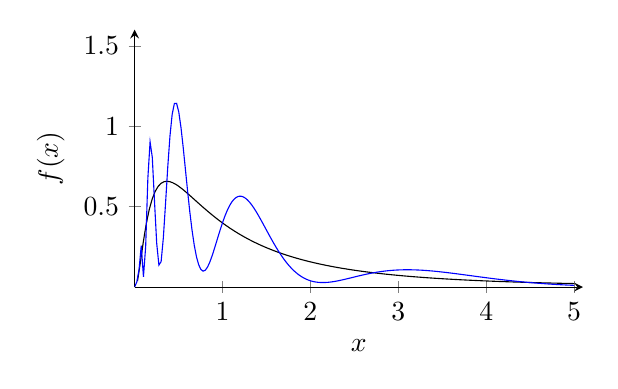
\begin{tikzpicture}
    \begin{axis}[
    axis lines=left,
    xlabel = $x$, ylabel = {$f(x)$},
    xmax = 5.1, xtick = {1, 2, 3, 4, 5},
    ymax = 1.6, ytick = {0.5, 1, 1.5},
    width=0.6\textwidth, height=0.4\textwidth]
    \addplot[domain=0:5, samples=150] {exp(-((ln(x))^2)/2)/(x*sqrt(2*pi))};
    \addplot[domain=0.001:5, samples=200, blue] {(1+0.8*sin(2*pi*(ln(\x)) r))*exp(-((ln(x))^2)/2)/(x*sqrt(2*pi))};
    \end{axis}
\end{tikzpicture}
    \captionof{figure}{Density of a log-normal distribution and its perturbed version.}
\end{center}

We note that these two seemingly different random variables have the same $r$-th moment. To see this, it suffices to evaluate the integral
\begin{equation*}
    \int_0^\infty x^{r-1} \exp\bracket{-\frac{(\ln x)^2}{2}} \sin(2\pi \ln x) \, dx, \quad r = 0,1,...
\end{equation*}
With a variable substitution of $s = \ln x$ (such that $ds = dx/x$), the integral equals to 
\begin{equation*}
    \int_{-\infty}^\infty \exp\bracket{(r-1)s} \exp\bracket{-\frac{s^2}{2}} \sin(2\pi s) \, dx
\end{equation*}
Notice the integrand is an $L^1$ function multiplied by $\sin(2\pi s)$. Therefore,  by the Riemann-Lebesgue lemma, the integral is zero, and the two random variables have the same moments!
\end{example}

\begin{exercise}[Computing the moments of log-normal distribution] What happened? We can compute at the $r$-th moments of the log-normal distribution:
\begin{enumerate}
\item Verify that if $\xi$ has a standard normal distribution ($\mathsf{N}(0,1)$), then $\exp(\xi)$ has a standard log-normal distribution. 
\item Use LOTUS to compute the $r$-th moment being equal to $\exp(r^2/2)$.
\end{enumerate}
Notice that the moments grows too fast for the characteristic function to be analytical (i.e. possess a Taylor series)!
\end{exercise}

\subsection{Inversion Formula}
The main objective of this section is to make the inversion formula for characteristic functions precise. Let us state the first part of inversion formula.

\begin{theorem}[Inversion formula I] \label{thm:inversion_I}
Let $\mu$ be a probability measure on $(\R,\B(\R))$ with its corresponding distribution $F(x) = \mu((-\infty,x])$ and characteristic function $\varphi(t) = \int_\R e^{itx} \, \mu(dx)$. If $a<b$ then
\begin{equation}
\lim_{T\to\infty} \frac{1}{2\pi} \int_{-T}^T \frac{e^{-ita}-e^{-itb}}{it} \varphi(t) \, dt = \mu((a,b)) + \frac{\mu(\set{a}) + \mu(\set{b})}{2}
\end{equation}
In particular when $\mu(\set{a}) = \mu(\set{b}) = 0$, so that $F$ is continuous at $a,b$, then 
\begin{equation}
    F(b) - F(a) = \mu((a,b]) = \mu((a,b)) = \lim_{T \to \infty} \frac{1}{2\pi} \int_{-T}^T \frac{e^{-ita} - e^{-itb}}{it} \varphi(t) \, dt;
\end{equation}
\end{theorem}

Before we begin proving this theorem, let us recall some facts about the integral of the sinc function. Define
\begin{equation}
S(T) = \int_0^T \frac{\sin x}{x} \, dx.
\end{equation}

We note that $S(T)$ is a differentiable function with $S(T) > 0$ whenever $T > 0$, and that

\begin{lemma}
\begin{equation}
S(+\infty) = \int_0^\infty \frac{\sin x}{x} = \frac{\pi}{2}
\end{equation}
\end{lemma}

This can be proven by standard calculus tricks, either by differentiation under integral or residue calculus. \footnote{There is an entire article of teaching you how to integrate a since function! See \url{https://www.wikihow.com/Integrate-the-Sinc-Function}.} We therefore know that $S(T)$ is a bounded function and $\sup_{T>0} S(T)$ exists. \\

We also note the following scaling formula 
\begin{equation}
\int_0^T \frac{\sin(kx)}{x} \, dx= \int_0^T \frac{\sin(kx)}{kx} \, d(kx) = S(kT), \quad k > 0,
\end{equation}
and that when $k < 0$, we have
\begin{equation}
\int_0^T \frac{\sin(kx)}{x} \, dx= -\int_0^T \frac{\sin(|k|x)}{x} \, dx = -S(|k|T).
\end{equation}

In terms of the $\sgn$ function ($\sgn = \chi_{(0,\infty)} - \chi_{(-\infty,0)}$), we have for all $k \in \R$,
\begin{equation}
\int_0^T \frac{\sin(kx)}{x} = \sgn(k) S(|k|T).
\end{equation}

Finally, provided that the sinc function is even, we know that
\begin{equation}
\int_{-T}^T \frac{\sin(kx)}{x} = 2\sgn(k) S(|k|T).
\end{equation}

We are now ready to prove the first inversion formula:

\begin{proof} (of inversion formula I, theorem \ref{thm:inversion_I})
So let's first evaluate for fixed $T$,
\begin{equation}
I_T = \int_{-T}^T \frac{e^{-ita}-e^{-itb}}{it} \varphi(t) \, dt = \int_{-T}^T \int_\R \frac{e^{-ita}-e^{-itb}}{it} e^{itx} \, \mu(dx) \, dt
\end{equation}
We note that the integrand is bounded uniformly in $(t,x)$ (except when $t = 0$, which is a removable singularity):
\begin{equation}
\abs{\frac{e^{-ita} - e^{-itb}}{it} e^{itx}} \leq \abs{\int_a^b e^{-its} \, ds} \leq |b-a|, \label{eq:exponent_integral_estimate}
\end{equation}
so the integrand is integrable. By Fubini's theorem, we may exchange the order of integration:
\begin{equation}
I_T = \int_\R \int_{-T}^T \frac{e^{-ita}-e^{-itb}}{it} e^{itx} \, dt \, \mu(dx) = \int_\R \int_{-T}^T \frac{e^{it(x-a)}-e^{it(x-b)}}{it} \, dt \, \mu(dx) 
\end{equation}
We focus on the inner integral. Since the domain is now symmetric, we may ignore the odd parts of the integral, so we have
\begin{equation}
I_T = \int_\R \int_{-T}^T \frac{\sin(t(x-a)) - \sin(t(x-b))}{t} \, dt \, \mu(dx) 
\end{equation}
We have established a few facts about integrals on since function, and we want to utilise them here. To do so, we have to justify the following exchange the order of limits when evaluating $I_\infty$:
\begin{equation*}
I_\infty = \lim_{T\to\infty} I(T) \overset{(?)}{=} \int_\R \lim_{T\to\infty} \underbrace{\int_{-T}^T \frac{\sin(t(x-a)) - \sin(t(x-b))}{t}}_{J_{T,x}} \, dt \, \mu(dx) 
\end{equation*}
and here we will use dominated convergence theorem (DCT). Notice we have
\begin{equation*}
    \abs{J_{T,x}} \leq \abs{\int_{-T}^T \frac{\sin(t(x-a))}{t}} + \abs{\int_{-T}^T \frac{\sin(t(x-b))}{t}} \leq 4 \sup_{T>0} S(T) < \infty,
\end{equation*}
which is integrable with respect to the probability measure $\mu$. Therefore the condition for DCT is satisfied. \\

Let us now tabulate the values of $J_{\infty,x}$ for different values of $x$:
\begin{table}[h]
    \centering
    \begin{tabular}{c|c|c|c}
       $x$  & $\displaystyle{\int_{-\infty}^\infty \frac{\sin(t(x-a))}{t} \, dt }$ &  $\displaystyle{\int_{-\infty}^\infty \frac{\sin(t(x-b))}{t} \, dt}$ & $J_{\infty, x}$\\
       \hline
       $x>b$ & $\pi$ & $\pi$ & 0 \\
       $x=b$ & $\pi$ & 0 & $\pi$ \\
       $a<x<b$ & $\pi$ & $-\pi$ & $2\pi$ \\
       $x=a$ & $0$ & $-\pi$ & $\pi$ \\
       $x<a$ & $-\pi$ & $-\pi$ & 0
    \end{tabular}
\end{table}

and therefore we have 
\begin{equation*}
    I_\infty = \int_{\set{a}} \pi d\mu + \int_{\set{b}} \pi d\mu + \int_{(a,b)} 2\pi d\mu = 2\pi \bracket{\frac{\mu(\set{a}) + \mu(\set{b})}{2} + \mu((a,b))},
\end{equation*}

which completes the proof.
\end{proof}

Let us also state another inversion formula for obtaining the measures of an atom.

\begin{theorem}[Inversion formula II] \label{thm:inversion_II}
Under the setting of the first inversion formula (theorem \ref{thm:inversion_I}), we have
\begin{equation}
\mu(\set{a}) = \lim_{T\to\infty}\frac{1}{2T} \int_{-T}^T e^{-ita} \varphi(t) \, dt
\end{equation}
\end{theorem}

\begin{proof}
The proof is as similar as above, so we will only give a sketch. We first let 
\begin{align*}
I_T := \frac{1}{2T} \int_{-T}^T e^{-ita} \varphi(t) \, dt &= \frac{1}{2T} \int_{-T}^T \int_\R e^{it(x-a)} \, d\mu \, dt \\
&\overset{\text{(Fubini)}}{=} \int_\R \frac{1}{2T} \int_{-T}^T e^{it(x-a)} \, dt \, d\mu \\
&= \int_{\R} \frac{e^{iT(x-a)} -e^{-iT(x-a)}}{2iT(x-a)} \, d\mu \quad \text{see \footnote{when $x = a$ then let the integrated be 1 by continuity, but it doesn't really matter that much.}} \\
&= \int_{\R} \frac{\sin(T(x-a))}{T(x-a)} \, d\mu.
\end{align*}
We note that the integrand is uniformly bounded by one, which is integrable, so by DCT we have
\begin{equation}
I_\infty = \int_\R \bracket{\lim_{T\to\infty} \frac{\sin(T(x-a))}{T(x-a)} \, d\mu}.
\end{equation}
But note that the integrand tends to one when $x = a$ as $T \to \infty$ and zero otherwise, so we have
\begin{equation}
I_\infty = \lim_{T\to\infty}\frac{1}{2T} \int_{-T}^T e^{-ita} \varphi(t) \, dt = \mu(\set{a}). 
\end{equation}
\end{proof}

\begin{corollary} \label{cor:cf_dist_one_to_one}
Probability distributions on $(\R, \B(\R))$ and characteristic functions are in one-to-one correspondence.
\end{corollary}

\begin{proof}
So let's say $\mu,\nu$ are two measures on $(\R,\B(\R))$ such that they have the same characteristic function. By the inversion formulas we see that $\mu((a,b)) = \nu((a,b))$ for any $a<b$. Since the collection of open intervals $\set{(a,b) \,|\, a < b}$ generates $(\R,\B(\R))$, we must have $\mu = \nu$.
\end{proof}

The final inversion formula concerns the absolute continuity of a probability measure $\mu$ with respect to the Lebesgue measure (i.e. whether a continuous density exists). It turns out that if its characteristic function $\varphi$ is integrable, then we may invert the Fourier transform in the following sense

\begin{proposition}[Inversion formula III]
If $\int_{-\infty}^\infty |\varphi(t)| \d t < \infty$, then the probability measure $\mu(x)$ has density $f(x)$, in the sense that the distribution function $F$ satisfies
\begin{equation} \label{eq:density}
    F(x) = \mu((-\infty,x]) = \int_{-\infty}^x f(y) \, dy,
\end{equation}
and that the density is given by
\begin{equation} \label{eq:L1_inversion}
    f(x) = \frac{1}{2\pi} \int_{-\infty}^\infty e^{-itx} \varphi(t) dt.
\end{equation}
\end{proposition}

We note that this inversion formula coincides with the $L^1$ inversion formula for Fourier transform: let $f \in L^1(\R)$ and its Fourier transform (which is $\varphi(-t)$ with $\varphi$ being the characteristic function of the measure as defined in \eqref{eq:density}) is in $L^1$, then \eqref{eq:L1_inversion} holds with the minus sign replaced by a plus sign.

\begin{proof}
Utilise inversion formula I (theorem \ref{thm:inversion_I}) and the estimate \eqref{eq:exponent_integral_estimate}, we have
\begin{equation}
\mu((a,b)) + \frac{\mu(\set{a}) + \mu(\set{b})}{2} = \lim_{T\to\infty} \frac{1}{2\pi} \int_{-T}^T \frac{e^{-ita}-e^{-itb}}{it} \varphi(t) \leq \frac{b-a}{2} \int_\R |\varphi(t)| \, dt \lesssim \Leb((a,b)).
\end{equation}
This proves that $\mu \ll \Leb$, so that $\mu$ possess a density and has no atoms. We now prove that the function given in \eqref{eq:L1_inversion} is a density of $\mu$: note that
\begin{equation}
\mu((x,x+h)) = \frac{1}{2\pi} \int_\R \bracket{\int_x^{x+h} e^{-ity} \, dy} \, \phi(t) \, dt \overset{\text{(Fubini)}}{=} \int_x^{x+h} \bracket{\frac{1}{2\pi} \int_\R e^{-ity} \phi(t) \, dt} \, dy
\end{equation}
So $\mu$ has density function $f$ as given in \eqref{eq:L1_inversion}. It is easy to show that $f$ is continuous (by, e.g. dominated convergence theorem).
\end{proof}

\begin{exercise}
Show that the function $f$ as defined above is continuous by dominated convergence theorem.
\end{exercise}

We may use the third inversion formula to find the characteristic function for even more distributions.
\begin{exercise} \label{ex:CF_Polya_Cauchy}
Let $\xi,\eta$ be a real-valued random variable.
\begin{enumerate}
    \item Find the characteristic function of $\xi$ if $\xi$ follows a triangular distribution with density
    \begin{equation}
        f(t) = (1-|t|)_+ := (1-|t|) \vee 0,
    \end{equation}
    then use the third inversion formula to show that the characteristic function of $\eta$ is $\varphi_\eta(t) = (1-|t|)_+$, where the $\eta$ follows a Polya's distribution \footnote{We follow the naming convention in \cite{Durrett}.} with density
    \begin{equation}
        f(t) = \frac{1-\cos t}{\pi t^2}.
    \end{equation}
    We will need this distribution to prove a theorem for the characterisation of characteristic function in section 6.4.
    \item Find the characteristic function of $\xi$ if $\xi$ follows a Laplace (bilateral exponential) distribution with density
    \begin{equation}
        f(t) = \exp(-|t|)/2,
    \end{equation}
    and hence find the characteristic function of $\eta$ if $\eta$ follows a Cauchy distribution with density
    \begin{equation}
        f(t) = (\pi(1+t^2))^{-1}.
    \end{equation}
\end{enumerate}
\end{exercise}

\subsection{Central Limit Theorems}
We are almost able to prove the Central Limit Theorem. We need to prove the final (and the most important) step, the Levi's continuity theorem, which says if 

\begin{theorem}[Levi's Continuity theorem] \label{thm:levi_continuity}
Let $\varphi_n(t)$ be the characteristic functions of a sequence of probability measures $\p_n$ with on $(\R,\B(\R))$ distribution functions $F_n$. Then
\begin{enumerate}
    \item If $\p_n \to \p_\infty$ weakly, where $\p_\infty$ is a measure on $(\R,\B(\R))$, then $\varphi_n(t) \to \varphi_\infty(t)$ \textbf{pointwise} for all $t \in \R$, where $\varphi_\infty$ is the characteristic function of $\mu_\infty$.
    \item If $\lim_{n \to \infty} \varphi_n(t)$ exists $\forall t \in \R$, and $\varphi_\infty(t) = \lim_{n \to \infty} \varphi_n(t)$ is \textbf{continuous} at $t=0$, then $\varphi_\infty(t)$ is a characteristic function of some probability measure $\p$ and $\p_n \to \p$ (weakly). 
    \item If $\varphi_n(t)$ corresponds to $\p_n$ and $\varphi_\infty(t)$ is a characteristic function corresponding to $\p_\infty$, then
    \begin{equation*}
        \varphi_n(t) \to \varphi_\infty(t)\, \, \forall t \in R \iff \p_n \to \p_\infty \text{ (weakly)}.
    \end{equation*}
\end{enumerate}
\end{theorem}

We note that statement (1) is a direct consequence of the definition of weak convergence when applied to $\Re[e^{it\xi}]$, $\Im[e^{it\xi}]$.

\begin{unexaminable}
To prove statements 2 and 3, we need the following estimates:
\begin{lemma}
If $\p$ is a probability measure on $(\R,\B(\R))$ with characteristic function $\varphi(t)$, then for all $\epsilon > 0$, 
\begin{equation} \label{eq:cf_tail_bound}
    \p(\set{x \,|\, |x| \geq 2/\epsilon}) \leq \frac{1}{\epsilon} \int_{-\epsilon}^\epsilon (1-\varphi(t)) \, dt
\end{equation}
\end{lemma}

This lemma shows that the tail of measure $\p$, hence the existence of moments, is determined by the smoothness of $\varphi$ at zero. The direct connections between the existence of moments and smoothness are established in section 6.1.

\begin{proof}
First note that for all $x \neq 0$,
\begin{equation}
\int_{-\epsilon}^\epsilon (1-e^{itx}) \, dt = 2\epsilon - \frac{e^{it\epsilon} - e^{-it\epsilon}}{ix} = 2u\bracket{1-\frac{\sin \epsilon x}{\epsilon x}}
\end{equation}
We therefore have
\begin{align*}
    \frac{1}{\epsilon} \int_{-\epsilon}^\epsilon (1-\varphi(t)) \, dt 
    &= \frac{1}{\epsilon} \int_{-\epsilon}^\epsilon \bracket{1 - \int_\R e^{itx} \, \mu(dx)} \, dt \\
    &= \frac{1}{\epsilon} \int_{-\epsilon}^\epsilon \int_\R (1-e^{itx}) \, \mu(dx) \, dt \\
    &\overset{\text{(Fubini)}}{=} \int_\R \bracket{\frac{1}{\epsilon} \int_{-\epsilon}^\epsilon (1-e^{itx}) \, dt} \, \p(dx) \\
    &= \int_\R 2 \underbrace{\bracket{1 - \frac{\sin \epsilon x}{\epsilon x}}}_{\geq 0} \, \p(dx) \\ 
    &\geq 2 \int_{-2/\epsilon}^{2/\epsilon} \bracket{1 - \frac{\sin \epsilon x}{\epsilon x}} \, \p(dx) \\
    &\geq 2 \int_{-2/\epsilon}^{2/\epsilon} \underbrace{\bracket{1 - \frac{1}{|\epsilon x|}}}_{\geq 1/2} \, \p(dx) \\
    &\geq \p(\set{x \,|\, |x| \geq 2/\epsilon})
\end{align*}
\end{proof}

We are now ready to prove statements 2 and 3 of the continuity theorem.

\begin{proof}
We really only need to prove the second statement. When this is proven, the third statement follows from this and the inversion theorem. \\ 

\textbf{We first prove that the sequence $(\p_n)$ is tight.} We are given that $\varphi_\infty$ is continuous at 0 and that $\varphi_\infty(0) = 1$, so for all $\epsilon > 0$, there is $u > 0$ small enough that for all $t \in [-u,u]$, $1 - \varphi_\infty(t) \leq \epsilon / 4$, and hence 
\begin{equation}
\frac{\epsilon}{2} \geq \frac{1}{u} \int_{-u}^u (1-\varphi_\infty(t)) \, dt \overset{\text{(DCT)}}{=} \lim_{n\to\infty} \frac{1}{u} \int_{-u}^u \bracket{1-\varphi_n(t)} \, dt.
\end{equation}
As a result, there is $n_0$ such that for all $n \geq n_0$ such that 
\begin{equation}
\p_n\bracket{\R\setminus [-2/u,2/u]} \leq \frac{1}{u} \int_{-u}^u (1-\varphi_n(t)) \, dt \leq \epsilon
\end{equation}
We may choose smaller $u$ such that the above inequality holds for all $n \geq 1$, and hence we see that $(\p_n)_{n\geq 1}$ is tight. By Prokhorov theorem, for any subsequence of $(\mu_n)_{n\geq 1}$, say $(\mu_{n_k})_{k\geq 1}$, there is a further subsequence that converges weakly to the measure $\nu$. We note that by statement (1) of continuity theorem and uniqueness of limits we know that $\varphi_\infty(t)$ is the characteristic function of $\nu$, which also shows that the limiting measure must be unique regardless of what subsequence we have chosen. \\

We finally note that $\p_n \to \nu$ weakly, otherwise there is a point $y \in \R\setminus U_F$, $F$ distribution function of $\nu$, so that there is a subsequence $(\mu_{n'_k})_{k\geq 1}$ such that $|F_{n'_k}(y) - F(y)| \geq \epsilon$ for all $k$, but by above arguments there is a further subsequence $(\mu_{n_{k_j}})_{j\geq 1}$ which converges to $\nu$, which is a contradiction!
\end{proof}
\end{unexaminable}

Once we have the Levi's continuity theorem, we also have the following central limit theorems (CLTs) for free.

\begin{theorem}[Central Limit Theorem for Independent Identically Distributed Random Variables]
Let $\xi_1, \xi_2, \dots $ be a sequence of independent identically distributed (nondegenerate) random variables with $\E[\xi_1^2]] < \infty$ and $S_n = \xi_1 + \cdots + \xi_n$. Then as $n \to \infty$
\begin{equation*}
    \p \bigg\{ \frac{S_n - \E[S_n]}{\sqrt{\V[S_n]}} \le x \bigg\} \longrightarrow \Phi(x) \equiv \frac{1}{\sqrt{2\pi}} \int_{-\infty}^x e^{-u^2/2} \d u \quad \forall x \in \R.
\end{equation*}
\end{theorem}
\begin{remark}
The result can also be written as 
\begin{equation*}
    \frac{S_n - \E[S_n]}{\sqrt{\V[S_n]}} \xrightarrow{d} \mathsf{N}(0,1).
\end{equation*}
\end{remark}
\begin{proof}
Set $m = \E[\xi_1]$, $\sigma^2 = \V[\xi_1]$, $\varphi(t) = \E[e^{it(\xi_1 - m)}]$.
If we put
\begin{equation*}
    \varphi_n(t) = \E\bigg[\exp \bigg(it \frac{S_n - \E[S_n]}{\sqrt{\V[S_n]}} \bigg)\bigg],
\end{equation*}
by independence 
\begin{equation*}
    \varphi_n(t) = \bigg[\varphi\bigg(\frac{t}{\sigma \sqrt{n}}\bigg)\bigg]^n.
\end{equation*}
Since $\E[\xi_1^2] < \infty$, we have by properties of characteristic functions (theorem above) that 
\begin{equation*}
    \varphi(t) = 1 - \frac{\sigma^2 t^2}{2} + o(t^2), \quad t \to 0.
\end{equation*}
So $\varphi_n(t) = [1 - t^2/(2n) + o(1/n)]^n \to e^{-t^2/2}$ for all $t \in \R$. This is the characteristic function of $\mathsf{N}(0,1)$ and so the result follows by continuity theorem.
\end{proof}

\subsubsection{Lindeberg-Feller Theorem}
With more delicate analysis, we may prove another central limit theorem, known as the Lindeberg-Feller theorem.

\begin{theorem}[Lindeberg CLT for independent random variables]
Let $\xi_1, \xi_2, \dots$ be a sequence of independent random variables on same probability space $(\Omega,\F,\p)$ with finite second moments $\E[\xi_j^2] < \infty$. Let 
$$m_j = \E[\xi_j], \quad \sigma_j^2 = \V[\xi_j] >0,\quad S_n = \xi_1 + \cdots + \xi_n \text{ and } D_n^2 = \sum_{j=1}^n \sigma_j^2.$$ 
Suppose that the \textbf{Lindeberg condition} is satisfied: for every $\varepsilon > 0$
\begin{equation} \label{eq:Lindeberg_original}
    \frac{1}{D_n^2}\sum_{k=1}^n \E\sqbracket{|\xi_k - m_k|^2 \chi_{\set{|\xi_k-m_k|\ge \varepsilon D_n}}} \overset{n\to\infty} \to 0.
\end{equation}
Then 
\begin{equation*}
    \frac{S_n - \E[S_n]}{D_n} \xrightarrow{d} \mathsf{N}(0,1).
\end{equation*}
\end{theorem}

The idea of proof is similar to the one proving CLT for iid random variables, but the proof itself is too cumbersome to be included in our notes. If interested you may refer to theorem 3.4.10 of \cite{Durrett}.

\begin{remark}[Other formulation of CLT] \label{rmk:other_CLT}
We note that some literature has different versions of the above Lindeberg Theorem. For instance, Durrett states in \cite{Durrett} that under the above setting, if the following version of the Lindeberg condition is satisfied: if $D_n^2 \to \sigma^2 \in (0,\infty)$ (i.e. finite and \textbf{not tending to zero}); and for all $\epsilon > 0$,
\begin{equation}
    \sum_{k=1}^n \E\sqbracket{|\xi_k - m_k|^2 \chi_{\set{|\xi_k-m_k|\ge \varepsilon}}} \overset{n\to\infty} \to 0,
\end{equation}
then
\begin{equation*}
S_n - \E[S_n] \xrightarrow{d} \mathsf{N}(0,\sigma^2)
\end{equation*}
We show that the new Lindeberg theorem $\implies$ original Lindeberg theorem, we first note that we may squeeze the following limits:
\begin{align*}
    \frac{1}{D_n^2} \sum_{k=1}^n \E\sqbracket{|\xi_k - m_k|^2 \chi_{\set{|x-m_k|\ge \varepsilon D_n}}} &\leq \frac{1}{D_n^2} \sum_{k=1}^n \E\sqbracket{|\xi_k - m_k|^2 \chi_{\set{|x-m_k|\ge \varepsilon D_1}}} \\
    &\leq \frac{1}{D_1^2} \sum_{k=1}^n \E\sqbracket{|\xi_k - m_k|^2 \chi_{\set{|x-m_k|\ge \varepsilon D_1}}} \overset{n\to\infty} \to 0.
\end{align*}
So the original Lindeberg condition is satisfied, and by the original Lindeberg theorem, we have
\begin{equation*}
    \frac{S_n - \E[S_n]}{D_n} \xrightarrow{d} \mathsf{N}(0,1).
\end{equation*}
Notice that we also have $D_n/\sigma \nearrow 1$ as $n \to \infty$, so by Slutsky's theorem (proposition \ref{prop:mult_of_weak_limits}), we have 
\begin{equation*}
    \frac{S_n - \E[S_n]}{\sigma} \xrightarrow{d} \mathsf{N}(0,1),
\end{equation*}
which yields our desire convergence. In fact, by rescaling the random variables, we know that if $d_n^2 := D_n^2 / n \to \sigma^2 / n$, and that 
\begin{equation}
    \frac{1}{n} \sum_{k=1}^n \E\sqbracket{|\xi_k - m_k|^2 \chi_{\set{|\xi_k-m_k|\ge \varepsilon \sqrt{n}}}} \overset{n\to\infty} \to 0,
\end{equation}
then 
\begin{equation*}
S_n - \E[S_n] \xrightarrow{d} \mathsf{N}(0,\sigma^2/n)
\end{equation*}
To prove the converse, we need to introduce an suitable array of random variables. Since this is unexaminable, we will defer the proof to the end of this section. The reason of noting such equivalence is that the Lindeberg condition is that we don't need to deal with the sum $D_n^2$, so the Lindeberg condition is now easier to handle.
\end{remark}

We turn our attention to some special cases in which the Lindeberg condition is satisfied and consequently, the central limit theorem is valid. One of the most prominent example is the Lyapunov condition.
\begin{corollary}[Lyapunov's CLT]
Assume the above settings, and in addition assume that the sequence $(\xi_k)_{\geq 1}$ satisfy the \textbf{Lyapunov condition}: there is some $\delta > 0$ such that as $n \to \infty$,
\begin{equation}
    \frac{1}{D_n^{2 +\delta}} \sum_{k=1}^n \E[|\xi_k - m_k|^{2+\delta}] \to 0.
\end{equation}
Then the sequence $(\xi_k)_{\geq 1}$ satisfies the Lindeberg condition, and central limit theorem hold.
\end{corollary}

\begin{proof}
Let $\varepsilon > 0$. Convince yourself that
\begin{align*}
    \E[|\xi_k - m|^{2+\delta}] 
    \geq \E\sqbracket{|\xi_k - m_k|^{2+\delta} \chi_{\set{|\xi_k-m_k| \ge \varepsilon D_n}}} 
    \geq \varepsilon^\delta D_n^\delta \E\sqbracket{|\xi_k - m_k|^{2+\delta} \chi_{\set{|\xi_k-m_k| \ge \varepsilon D_n}}},
\end{align*}
and conclude that 
\begin{equation*}
    \frac{1}{D_n^2}\sum_{k=1}^n \int_{\{x: |x-m_k| \ge \varepsilon D_n\}} (x - m_k)^{2}  \d F_k(x) \le \frac{1}{\varepsilon^\delta} \frac{1}{D_n^{2 + \delta}} \sum_{k=1}^n \E[|\xi_k - m_k|^{2 + \delta}].
\end{equation*}
Consequently, the Lyapunov condition implies the Lindeberg condition.
\end{proof}

We also note the following special case, with the proof being left as an exercise.
\begin{exercise} \label{ex:Lindeberg_for_bounded_rv}
Under the above settings, suppose that there exists $K$ such that for all $n \ge 1$
\begin{equation*}
    |\xi_k| \le K < \infty, \quad \forall k,
\end{equation*}
and that $D_n \to \infty$ as $n \to \infty$, then the sequence $(\xi_k)_{k\geq 1}$ also implies Lindeberg condition.
\end{exercise}

\begin{unexaminable}
Recall the setup of array of independent random variables in subsubsection 4.2.4, i.e. random variables $\xi_{n,k}$ with $n$ being row index and $1 \leq k \leq n$, so that on each selected row $n$ we have $\xi_{n,k}$ mutually independent. With this setup, we may state the full version of the Lindeberg theorem:
\begin{theorem}[Lindeberg CLT for array of random variables]
Let $(\xi_{n,k})_{n\geq 1, \, 1\leq k\leq n}$ be an array of random variables, each of them having finite second moments. Let 
\begin{equation*}
m_{n,k} = \E[\xi_{n,k}], \quad S_n = \sum_{k=1}^n \xi_{n,k}, \quad D_n^2 = \sum_{k=1}^n \V[\xi_{n,k}^2].
\end{equation*}
Suppose that the following Lindeberg condition holds: for every $\varepsilon > 0$, 
\begin{equation}
    \frac{1}{D_n^2}\sum_{k=1}^n \E\sqbracket{|\xi_{n,k} - m_{n,k}|^2 \chi_{\set{|\xi_{n,k}-m_k|\ge \varepsilon D_n}}} \overset{n\to\infty} \to 0.
\end{equation}
Then 
\begin{equation*}
    \frac{S_n - \E[S_n]}{D_n} \xrightarrow{d} \mathsf{N}(0,1).
\end{equation*}
Alternatively, if the following version of Lindeberg condition holds: $D_n^2 \nearrow \sigma^2 \in (0,\infty)$ as $n \to \infty$, and that 
\begin{equation}
    \sum_{k=1}^n \E\sqbracket{|\xi_{n,k} - m_{n,k}|^2 \chi_{\set{|\xi_{n,k}-m_k|\ge \varepsilon}}} \overset{n\to\infty} \to 0,
\end{equation}
then 
\begin{equation*}
    S_n - \E[S_n] \xrightarrow{d} \mathsf{N}(0,\sigma^2).
\end{equation*}
\end{theorem}

The Lindeberg CLT for independent random variables $(\xi_k)_{k\geq 1}$ immediate follows from the above Lindeberg CLT for array of random variables by setting $\xi_{n,k} \equiv \xi_k$ for all $n$. The above generalisation of Lindeberg CLT allows us to translate in between the original Lindeberg's CLT and the Durrett's formulation of Lindeberg CLT in \cite{Durrett}: \footnote{Thanks for the StackExchange post: \url{https://math.stackexchange.com/questions/3917501/lindeberg-feller-alternative-formulation-in-durrett}.}

\begin{remark}[continued from remark \ref{rmk:other_CLT}]
We note that the implication from the new Lindeberg condition to the original Lindeberg condition can be seen as followed: under the above setting, we define the new random variables $\eta_{n,k} := (\xi_{n,k} - m_{n,k})/D_n$. Then for this new array of random variables, we have $\tilde{D}_{n}^2 := \sum_{k=1}^n \V[\eta_{n,k}] \equiv 1$. Moreover, as $n\to\infty$,
\begin{equation}
    \frac{1}{D_n^2}\sum_{k=1}^n \E\sqbracket{|\xi_{n,k} - m_{n,k}|^2 \chi_{\set{|\xi_{n,k}-m_k|\ge \varepsilon D_n}}} = \sum_{k=1}^n \E\sqbracket{|\eta_{n,k}|^2 \chi_{\set{|\eta_{n,k}|\ge \varepsilon}}} \to 0,
\end{equation}
so
\begin{equation*}
    \tilde{S}_n := \sum_{k=1}^n \eta_{n,k} = \frac{S_n - \E[S_n]}{D_n} \xrightarrow{d} \mathsf{N}(0,1)
\end{equation*}
as desired. In particular, this prove the converse in remark \ref{rmk:other_CLT}.
\end{remark}

The corresponding version of Lyapunov's CLT for an array of random variable is as followed:
\begin{corollary}[Lyapunov's CLT]
Assume the above array setup, and in addition assume that the sequence $(\xi_k)_{\geq 1}$ satisfy the \textbf{Lyapunov condition}: there is some $\delta > 0$ such that as $n \to \infty$,
\begin{equation}
    \frac{1}{D_n^{2 +\delta}} \sum_{k=1}^n \E[|\xi_{n,k} - m_{n,k}|^{2+\delta}] \to 0.
\end{equation}
Then the sequence $(\xi_k)_{\geq 1}$ satisfies the Lindeberg condition, and central limit theorem hold.
\end{corollary}

As a final note, the Lindeberg CLT admits a partial converse, as discovered by Feller. This theorem is usually combined with the Lindeberg CLT to form the Lindeberg-Feller theorem, although this theorem is of little use in our course.
\begin{theorem}[Feller's theorem]
assuming the above setup, and in addition we have $(S_n - \E[S_n])/D_n \xrightarrow{d} \mathsf{N}(0,1)$ and $(\max_i \V[\xi_{n,k}])/D_n^2 \to 0$ (i.e. for each row there isn't a "dominating" random variable $\xi_{n,k}$ with variance dominating the sum variance along the row, then the Lindeberg condition holds. 
\end{theorem}
\end{unexaminable}

\subsubsection{Counterexample of CLT when the random variable is not squared integrable}
Does CLT still hold even when $\E[\xi_1^2] = \infty$? Let $\xi_1, \xi_2, \dots$ be i.i.d. with Cauchy distribution, i.e. with density
\begin{equation*}
    f = \frac{\theta}{\pi(x^2 + \theta^2)}, \quad \theta>0.
\end{equation*}
Then, as shown in question 2 of exercise \ref{ex:CF_Polya_Cauchy}, we have
\begin{equation*}
    \varphi_{\xi_1}(t) = e^{-\theta |t|}, t \in \R,
\end{equation*}
which implies that 
\begin{equation*}
    \varphi_{S_n/n} (t) = (e^{-\theta|t|/n})^n = e^{-\theta|t|},
\end{equation*}
and thus $S_n/n$ also has the Cauchy distribution (instead of Normal)!

\subsection{Berry-Esseen Inequality}
The Central Limit Theorem for iid random variables and question 1 of exercise \ref{ex:uniform_conv_of_dist} implies that, if $F_n(x)$ is the distribution function of the random variable $(S_n - \E[S_n])/\sqrt{\V[S_n]}$, then we have
\begin{equation}
\sup_{x} |F_n(x) - \Phi(x)| \overset{n\to\infty}\to 0.
\end{equation}

In what rate does the LHS decay? It turns out that if $(\xi_k)_{k\geq 1}$ are iid with $\xi_1 \in L^3$, then we have the following Berry-Esseen inequality.
\begin{theorem}[Berry-Esseen Inequality]
Let $\xi_1, \xi_2, \dots$ be a sequence of independent and identically distributed random variables with $\E[|\xi_1|^3] < \infty$. Then
\begin{equation*}
    \sup_x \bigg| \p\bigg( \frac{S_n - \E[S_n]}{\sqrt{\V[S_n]}} \le x\bigg) - \Phi(x) \bigg| \le C\frac{\E[|\xi_1 - \E[\xi_1]|^3]}{\sigma^3\sqrt{n}},
\end{equation*}
where the absolute constant $C$ satisfies the inequality
\begin{equation*}
    \frac{1}{\sqrt{2\pi}} \le C < 0.8.
\end{equation*}
\end{theorem}

There are many proofs to this famous theorem, but we do not intend to include any of them as they are too technical for this course. In fact, finding the optimal constant $C$ is an active research area, and mathematicians continue to develop different tools in making the Berry-Esseen Inequality even sharper. Nevertheless, we know that the rate $\ord(1/\sqrt{n})$ is optimal, and that $C \geq 1/\sqrt{2\pi}$.

\begin{remark}
$O(1/\sqrt{n})$ is optimal. Indeed, let $\xi_1, \xi_2, \dots$ be independent and identically distributed Bernoulli random variables, 
\begin{equation*}
    \p(\xi_k = 1) = \p(\xi_k = -1) = \frac12.
\end{equation*}
Then by symmetry,
\begin{equation*}
    2\p\bigg(\sum_{k=1}^{2n} \xi_k < 0\bigg) + \p\bigg(\sum_{k=1}^{2n} \xi_k = 0\bigg) = 1
\end{equation*}
and therefore,
\begin{equation*}
    \bigg|\p\bigg(\sum_{k=1}^{2n} \xi_k < 0\bigg) - \frac12 \bigg| = \frac12 \p\bigg(\sum_{k=1}^{2n} \xi_k = 0\bigg) = \frac12 \binom{2n}{n} \frac{1}{2^{2n}} \sim \frac{1}{2\sqrt{\pi n}} = \frac{1}{\sqrt{2\pi}\sqrt{2n}}.
\end{equation*}
Then $\E[|\xi_1|^3] = 1 = \sigma_1$, so the theorem cannot be improved in terms of $O(1/\sqrt{n})$ and $C \ge \frac{1}{\sqrt{2\pi}}$.
\end{remark}

\subsection{More about constructing characteristic function}
The following theorems determine whether a function $\varphi$ is a characteristic function of some measure on $\R$, and if so, whether we can easily construct the underlying measure. The constructions are usually difficult, and therefore are not usually covered in great detail. Nevertheless, the proofs in this section serve as great examples of using tools developed in the previous chapter. For further discussions please refer to \cite{characteristic_function}.

\subsubsection{Bochner-Khinchin Theorem}
\begin{theorem}[Bochner-Khinchin]
Let $\varphi(t)$ be continuous, $t\in \R$, with $\varphi(0) = 1$. A necessary and sufficient condition that $\varphi(t)$ is a characteristic function is that it is positive semi-definite, i.e. that for all real $t_1, \dots, t_n$ and all complex $\lambda_1, \dots, \lambda_n$, $n=1,2,\dots$,
\begin{equation*}
    \sum_{j,k = 1}^n \varphi(t_j - t_k)\lambda_j \overline{\lambda}_k \ge 0.
\end{equation*}
\end{theorem}

To show necessity, we note that if $\varphi$ is a characteristic function of a real-valued random variable $\xi$, then 
\begin{equation*}
    \sum_{j,k = 1}^n \varphi(t_j - t_k)\lambda_j \overline{\lambda}_k \ge 0 = \E\sqbracket{\eta\bar{\eta}} = \E[|\eta|^2] \geq 0, \quad \eta = \sum_{j=1}^n \lambda_j e^{t_j \xi}. 
\end{equation*}

The fact that one can construct a probability measure with a positive semi-definite characteristic function is a deep fact in Fourier analysis, and the proof for general cases is beyond our scope. The case for $\varphi$ being integrable is covered in the third inversion formula.

\subsubsection{Polya's Criterion}
\begin{theorem}[Polya's criterion]
Let a continuous even real-valued function $\varphi(t)$ satisfy $\varphi(t) \ge 0$, $\varphi(0) = 1$, $\varphi(t) \to 0$ as $t \to \infty$ and let $\varphi(t)$ be convex on $0 \le t < \infty$ (hence also on $(0, \infty)$). Then $\varphi(t)$ is a characteristic function.
\end{theorem}

As an observation, we note that the function $\varphi(t)$ must be strictly decreasing over $[0,\infty)$ (see Lemma 2.5 of \cite{convex_decay}). To see this, we let $0<r<s$, then there is $t_0 > s$ such that $0<f(t_0)<f(r)/2$. By convexity, we have
\begin{equation*}
    f(s) \leq \frac{f(t_0) - f(r)}{t_0 - r} (s - r) + f(r) < f(r).
\end{equation*}

The Polya's criterion relies on the following simple observation of characteristic function.
\begin{exercise}[Convex combination of characteristic function]
Let $\varphi_k(t)$, $k=1,2,\dots$ be characteristic functions and let the nonnegative numbers $\lambda_k$ satisfy $\sum_{k=1}^n \lambda_k = 1$. Show that for all $n \in \Z_{\geq 1}$
\begin{equation*}
    \sum_{k=1}^n \lambda_k \varphi_k(t)
\end{equation*}
is a characteristic function. Extend the above result for $n = \infty$.
\end{exercise}

As it turns out, any function $\varphi(t)$ can be approximated by a convex combination of the characteristic function of a Polya's distribution $\varphi(t) = (1-|t|)_+$. Let us, therefore, follow the arguments in \cite{Billingsley} and complete the proof of Polya's criterion.

\begin{unexaminable}
\begin{exercise} \label{ex:Polya_polygon}
Consider a function $\varphi(t)$ as constructed as below: suppose that $d_1, d_2, ... > 0$ with $\sum_{k\geq 1} d_k = \infty$, and $s_1 \geq s_2 \geq ... \geq 0$ such that $s_k \searrow 0$ and $\sum_{k=1}^\infty s_k d_k = 1$. We further let $d_0 = 0$, $s_0 = 1$ for convenience, and $D_n = \sum_{k=0}^n d_k$. Define $\varphi(t)$ as 
\begin{equation}
    \varphi(t) = \sum_{n\geq 0} \bracket{1 - \bracket{\sum_{k=0}^n s_k d_k} - s_{n+1} (d_{n+1}-|t|)} \chi_{[D_n, D_{n+1})}(|t|)
\end{equation}
\begin{center}
    \begin{tikzpicture}
    \begin{axis}[
    axis lines=left,
    xlabel = $t$, ylabel = {$\varphi(t)$},
    xmin = 0, xmax = 3.3, xtick = {0, 1, 2, 3}, 
    ymin = 0, ymax = 1.3, ytick = {0, 1/4, 1/2, 1},
    xticklabels={$0$, $D_1$, $D_2$, $D_3$},
    yticklabels={$0$, $1-s_1d_1 - s_2d_2$, $1-s_1d_1$, $1$}, 
    width=0.4\textwidth, height=0.4\textwidth]
    \draw (0,1) -- (1,1/2);
    \draw [dashed] (1,1/2) -- (2,0);
    \draw (1,1/2) -- (2,1/4);
    \draw [dashed] (2,1/4) -- (3,0);
    \draw (2,1/4) -- (3,1/8);
    \end{axis}
\end{tikzpicture}
    \captionof{figure}{Approximation of a decaying convex function.}
\end{center}
The graph of $\varphi(t)$ for $t\geq 0$ is shown above with thick lines. Let further that $\varphi_0(t) := (1-|t|)_+$ be the characteristic function of the Polya's distribution. Show that $\varphi(t)$ is a convex combination of the characteristic function $\varphi_0(t/t_n)$ for some sequence $t_1, t_2, ...$, and hence is itself a characteristic function.
\end{exercise}

\begin{hint}
We may first assume that $s_k = 0$ for $k > m$ and prove the above statement by induction on $m$, before sending $m \to \infty$ in a suitable way. For the case when $s_k = 0$ for $k > m$ we have $\sum_{k=1}^m d_k s_k = 1$, and that $\varphi(t)$ is a \textbf{linear} combination of the functions $\varphi(s_1 t), ... \varphi(s_m t)$. We may therefore let
\begin{equation}
    \varphi(t) = \sum_{i=1}^m \lambda_i \varphi(s_i t)
\end{equation}
for some $\lambda_1,...,\lambda_m$, and solve for $\lambda_i$'s by considering the case when $t = D_1,...,D_m$. Finally, show that $\lambda_1 + ... + \lambda_m = 1$.
\end{hint}

\begin{remark}
The construction above indicates that two different distributions might possess characteristic functions which agree with each other over a finite interval containing $0$.
\end{remark}

\begin{exercise}
Complete the proof of Polya's criterion by noting that any function satisfying Polya's criterion itself can be approximated by functions in the form as in exercise \ref{ex:Polya_polygon}.
\end{exercise}

\begin{hint}
A suggested candidate for the sequence of functions is as followed: define $\varphi_n(t)$ on $t \in [0,n]$ so that it is piecewise linear and passes through the points $(0,1), (1/n, \varphi(1/n)), (2/n, \varphi(2/n))...$, and extend by $\varphi_n(-t) = \varphi_n(t)$. The slope for each line segment decreases due to the convexity of $\varphi(t)$, so that $\varphi(t)$ is continuous and possesses a right derivative $\varphi'(t)$ with $|\varphi'(|t|)| \to 0$ as $t \to \infty$.\\

Uniform convergence can be shown as follow: fix $\epsilon > 0$, then there exists $M,N$ such that $\varphi_n(t), \varphi(t) < \epsilon$ for all $n \geq N$, uniformly for all $t$ with $|t|>M$. Then in the interval $[-M,M]$, show that $\varphi_n(t) \to \varphi(t)$ uniformly.
\end{hint}
\end{unexaminable}

% This theorem provides a very convenient method of constructing characteristic functions. Examples are
% \begin{align*}
%     \varphi_1(t) &= e^{-|t|}\\
%     \varphi_2(t) &= \begin{cases}
%     1 - |t| & |t| \le 1,\\
%     0 & |t| > 1.
%     \end{cases}
% \end{align*}
% Another is the function $\varphi_3(t)$ drawn below. On $[-a, a]$, as, the function $\varphi_3(t)$ coincides with $\varphi_2(t)$. However, the corresponding distribution functions $F_2$ and $F_3$ are evidently different.

% \begin{center}
% 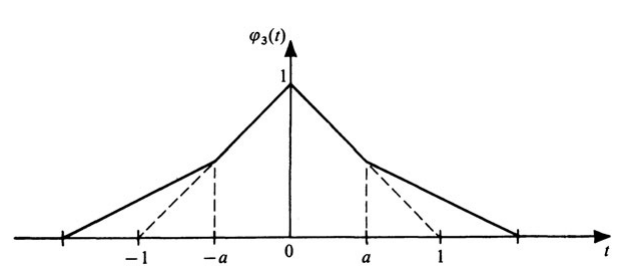
\includegraphics[scale=0.7]{figures/charact_functions.png}
% \end{center}

% This example shows that in general two characteristic functions can be the same on a finite interval without their distribution functions being
% the same.

\subsubsection{Marcinkiewicz Theorem}
\begin{theorem}[Marcinkiewicz's Theorem] \label{thm:Marcinkiewicz}
If a characteristic function $\varphi(t)$ is of the form $e^{p(t)}$, where $p(t)$ is a polynomial, then this polynomial is of degree at most $2$.
\end{theorem}

\begin{example}
As a quick example, $e^{-t^4}$ is not a characteristic function of any real-valued random variables.
\end{example}

\begin{unexaminable}
Let us prove a simpler version of Marcinkiewicz's theorem, which assumes $p(t) = t^3 q(t)$ for polynomial $q(t)$. Recall that the first and second derivatives of the characteristic function represent the first and second moments. Therefore, 

\begin{exercise}[see (\cite{Durrett}, exercise 3.3.16)]
Show that if $\varphi(t)$ is the characteristic function of the real-valued random variable $\xi$ such that $\lim_{t\to 0 } (\varphi(t) - 1)/t^2 = c > -\infty$, then $\E[\xi] = 0$ and $\E[\xi^2] = -2c < \infty$. In particular, if $\varphi(t) = 1+o(t^2)$, then $\E[\xi^2] = 0$ (with variance = 0) and $\varphi(t) = 1$.
\end{exercise}

So if $\varphi(t)$ is indeed a characteristic function, then by Taylor expansion we have $\varphi(t) = 1+o(t^2)$, so $\varphi(t) \equiv 1$ and $q(t) \equiv 0$. The actual proof of Marcinkiewicz's theorem is beyond our scope.
\end{unexaminable}

\subsubsection{Cumulants}
\begin{definition}
If there exists an expansion 
\begin{equation*}
    \log \varphi_\xi(t) = \sum_{k=0}^n \frac{(it)^k}{k!} s_k + o(|t|^n), \quad t \to 0,
\end{equation*}
then the coefficients $s_k$ are called \textbf{cumulants} of $\xi$.
\end{definition}
\begin{exercise}
Show that 
\begin{equation*}
    \E[\xi] = s_1, \quad \V[\xi] = s_2.
\end{equation*}
\end{exercise}

\begin{remark}
\begin{itemize}
    \item[]
    \item If $\xi \sim N(m, \sigma^2)$ then
    \begin{equation*}
        s_1 = m, \quad s_2 = \sigma^2, \quad s_k = 0, \quad k\ge3.
    \end{equation*}
    \item In general, by Marcinkiewsicz's Theorem if for a random variable $\xi$ there exists $n$ such that $s_k = 0,$ for all $k \ge n$, then also $s_k = 0$ for all $k \ge 3$ and $\xi \sim N(s_1, s_2)$.
\end{itemize}
\end{remark}

\subsubsection{Degenerate distributions}
The following theorem shows that a property of the characteristic function of a random variable can lead to a non-trivial conclusion about the nature of the random variable
\begin{theorem}
Let $\varphi(t)$ be a characteristic function of $\xi$.
\begin{enumerate}
    \item If $|\varphi(t_0)| = 1$ for some $t_0 \ne 0$, then $\xi$ is concentrated at the points $a + nh$, $h = 2\pi/t_0$, for some $a$, that is,
    \begin{equation*}
        \sum_{-\infty}^\infty \p(\xi = a + n h) = 1,
    \end{equation*}
    where $a$ is a constant.
    \item If $|\varphi(t)| = |\varphi(\alpha t)| = 1$ for two different points $t$ and $\alpha t$, where $\alpha$ is irrational, then $\xi$ is degenerate, that is 
    \begin{equation*}
        \p(\xi = a) = 1,
    \end{equation*}
    where $a$ is some constant.
    \item If $|\varphi(t)|\equiv 1$, then $\xi$ is degenerate.
\end{enumerate}
\end{theorem}
\begin{proof}
\begin{enumerate}
    \item If $|\varphi(t_0)| = 1$, $t_0 \ne 0$, there is a number $a$ such that $\varphi(t_0) = e^{i t_0 a}$. Then
    \begin{align*}
        e^{i t_0 a} &= \int_{-\infty}^\infty e^{i t_0 x} \d \, F(x) \implies 1 = \int_{-\infty}^\infty e^{i t_0 (x-a)} \d \, F(x) \implies \\
        1 &= \int_{-\infty}^\infty \cos{ t_0 (x-a)} \d \, F(x) \implies \int_{-\infty}^\infty 1 - \cos{ t_0 (x-a)} \d \, F(x) = 0.
    \end{align*}
    Since $1 - \cos{t_0(x-a)} \ge 0$, it follows that 
    \begin{equation*}
        1 = \cos t_0(x-a) \quad (\p\text{-a.s.}).
    \end{equation*}
    \item If follows from $|\varphi(t)| = |\varphi(\alpha t)| = 1$ and from the previous statement that
    \begin{equation*}
        \sum_{n=-\infty}^{\infty} \p(\xi = a + \frac{2\pi}{t}n) = \sum_{m=-\infty}^{\infty} \p(\xi = b + \frac{2\pi}{\alpha t} m) = 1.
    \end{equation*}
    If $\xi$ is not degenerate, then there must be at least two common points:
    \begin{equation*}
        a + \frac{2\pi}{t} n_1 = b + \frac{2\pi}{ \alpha t} m_1, \quad a + \frac{2\pi}{t} n_2 = b + \frac{2\pi}{ \alpha t} m_2,
    \end{equation*}
    in the sets 
    \begin{equation*}
        \bigg\{ a + \frac{2\pi}{t}n, n=0, \pm 1, \dots \bigg\} \quad \text{and} \quad \bigg\{ b + \frac{2\pi}{\alpha t}m, m=0, \pm 1, \dots \bigg\},
    \end{equation*}
    whence 
    \begin{equation*}
        \frac{2\pi}{t}(n_1 - n_2) = \frac{2\pi}{\alpha t} (m_1 - m_2),
    \end{equation*}
    and this contradicts the assumption that $\alpha$ is irrational. Conclusion $3.$ follows from $2.$
\end{enumerate}
\end{proof}
\begin{exercise}
\begin{enumerate}
    \item[]
    \item Let $\varphi(t)$ be a characteristic function. Show that the following are also characteristic functions:
    \begin{equation*}
        |\varphi(t)|^2, \quad e^{\lambda(\varphi(t) - 1)}, \quad \lambda \ge 0, \quad \int_0^1 \varphi(u t) \d u, \quad  \int_0^\infty e^{-u} \varphi(u t) \d u
    \end{equation*}
    \item Let $X$ and $Y$ be independent identically distributed random variables with zero mean and unit variance. Prove using characteristic functions that if the distribution $F$ of $(X+Y)/\sqrt{2}$ is the same as that of $X$ and $Y$, then $F$ is the normal distribution.
    \item Let $\xi$ be an integer-valued random variable and $\varphi_\xi(t)$ be its characteristic function. Show that
    \begin{equation*}
        \p(\xi = k) = \frac{1}{2\pi} \int_{-\pi}^\pi e^{-ikt} \varphi_\xi(t) \d t, \quad k = 0, \pm 1, \pm 2, \dots
    \end{equation*}
    \item Show that if $\varphi(t)$ is a characteristic function, then $\Re[\varphi(t)]$ is also a characteristic function, but $\Im[\varphi(t)]$ is not.
\end{enumerate}
\end{exercise}
\newpage
\section{Almost Sure Convergence of Random Series}
This chapter is to deal with almost sure convergence of random series. A large part of this chapter is devoted to Kolmogorov's proof of the Strong Law of Large Number. We will also cover some other fundamental results like the Kolmogorov's 0-1 law and the law of iterated logarithm. 

\subsection{Important Zero-One Laws}
To begin, let us study a few zero-one laws in probability theory. A zero-one laws states that if an event $A$ in a probability space satisfies certain conditions, then $A$ must be trivial event, i.e. the probability of $A$ must be of probability zero or one. Zero-one laws provide an important shortcuts in establishing "almost sure" statements, including almost-sure convergence. 
\begin{example}
If we prove that an event satisfies the conditions for a particular zero-one law, and that the event has non-zero probability, then it must has probability one.
\end{example}

\subsubsection{Borel-Cantelli Lemma}
Perhaps the example with the easiest proof is the Borel-Cantelli lemma, which you might have seen in elementary probability classes. To proof this important lemma, assume $A_n$ be sequences of events (elements from the $\sigma$-algebra of a probability space $(\Omega, \F, \p)$). Recall the following events:

\begin{definition}[Infinitely often and eventually events] Define:
\begin{itemize}
    \item Infinitely often events:
    \begin{equation}
        \limsup_{n \to \infty} A_n = \bigcap_{n=1}^\infty \bigcup_{k \ge n} A_k = \{ \omega \in \Omega : \omega \in A_m \text{ for infinitely many }m \}
    \end{equation}
    If $\omega \in \limsup_{n \to \infty} A_n$, we say that $A_n$ occurs infinitely often (i.o.).
    \item Eventually (all except finitely often):
    \begin{equation}
        \liminf_{n \to \infty} A_n = \bigcup_{n=1}^\infty \bigcap_{k \ge n} A_k = \{\omega \in \Omega \,|\, \exists \, m_0(\omega) \text{ such that }\omega \in A_m \text{ for all }m \ge m_0(\omega)\}
    \end{equation}
    If $\omega \in \limsup_{n \to \infty} A_n$, we say that $A_n$ occurs eventually (or almost except finitely often, a.e.f.o).
\end{itemize}
\end{definition}

\begin{exercise}
\begin{enumerate}
\item Try to give a precise interpretation of the descriptions "infinitely often" and "eventually", "limit infimum" and "limit supremum".
\textit{Hint}: convince yourself that
\begin{equation}
\chi_{\liminf_{n\to\infty} A_n}
\end{equation}
\item Show that
\begin{equation}
\p\bracket{\liminf_{n\to\infty} A_n} \leq \liminf_{n\to\infty} \p(A_n)
\end{equation}
and prove a similar statement for the probability of event $\liminf_{n\to\infty} A_n$.
\item Describe the complement of $\limsup_{n\to\infty} A_n$.
\end{enumerate}
\end{exercise}

We are now ready to prove the Borel-Cantelli Lemma. 
\begin{theorem}[Borel-Cantelli Lemma]
\begin{enumerate}
    \item[]
    \item If $\sum_{n=1}^\infty \p(A_n) < \infty$ then $\p(A_n \,\, i.o.) = 0$.
    \item If $\sum_{n=1}^\infty \p(A_n) = \infty$ and $A_n$ are mutually independent then $\p(A_n \,\, i.o.) = 1$.
\end{enumerate}
\end{theorem}

We note that if an event $A$ can be expressed as the lim-sup of an infinite sequence of mutually independent events $(A_n)_{n\geq 1}$, then Borel-Cantelli Lemma states that the probability of $A$ must be either zero and one. As a result, Borel-Cantelli lemma is a zero-one law.

\begin{proof}
\begin{enumerate}
    \item[]
    \item By continuity of measure we have
    \begin{equation*}
        \p (A_n \,\, i.o.) = \lim_{n\to\infty} \p \bigg(\bigcup_{k\ge n} A_k \bigg) \le \lim_{n \to \infty} \sum_{k=n}^\infty \p(A_k) = 0.
    \end{equation*}
    \item Consider $\{A_n \, \, i.o. \}^c = \big\{ A_n^c \,\,  ev.  \big\} = \bigcup_{n=1}^\infty \bigcap_{k \ge n} A_k^c$. We have
    \begin{equation*}
        1 - \p(A_n \, \, i.o.) = \lim_{n\to \infty} \p\bigg( \bigcap_{k\ge n} A_k^c \bigg).
    \end{equation*}
    Also, 
    \begin{equation*}
        \p\bigg( \bigcap_{k\ge n} A_k^c \bigg) = \prod_{k \ge n}\p(A_k^c).
    \end{equation*}
    Note that $\log(1-x) \le -x$ for $x \in [0, 1)$, and thus 
    \begin{equation*}
        \log\p\bigg( \bigcap_{k\ge n} A_k^c \bigg) = \log \prod_{k\ge n}(1 - \p(A_k)) \le -\sum_{k \ge n}\p(A_k) = -\infty,
    \end{equation*}
    i.e. $\p\bigg( \bigcap_{k\ge n} A_k^c \bigg) = 0$ for all $n$.
\end{enumerate}
\end{proof}

Here we give an example of an application of Borel Cantelli lemma.

\begin{example}[Infinite Monkey Theorem]
For Lebesgue almost every real number in $[0,1]$, its binary expansion contains any finite string of $\set{0,1}$ infinitely many times. To see that, assume the desired string to be $(x_1,...,x_m)$. We consider the sequence of events on $([0,1], \B([0,1]), \Leb)$:
\begin{equation*}
A_n := \set{\omega \,|\, \xi_{nm+1}(\omega) = x_1, \xi_{nm+2}(\omega) = x_2, ..., \xi_{nm+m}(\omega) = x_m}, \quad n \geq 0
\end{equation*}
where $\xi_k$ are the Radamacher functions as constructed in section 4.1 corresponding to the $k$-th digit of the binary expansion of $\omega \in [0,1)$. The events $A_n$ represents that the desired string appears starting from digit $nm+1$, which are mutually independent given that the Radamacher functions are independent as well. Also note that $\sum_{n\geq 1} \lambda(A_n) = \infty$, so $\Leb(\set{A_n \text{ i.o.}}) = 1$ as desired. \\

There are many versions of this theorem, with one saying that if we provide an infinite amount of time for a monkey to hit keys on a typewriter keyboard randomly, then it is almost certain that the monkey will type a given finite string of characters infinitely often. The proof of this statement is exactly the same, except here we look at $[0,1)$ with a 26-adic expansion. However, the Borel-Cantelli lemma does not provide information on how much time it would require for a monkey to complete the entire string...

\begin{center}
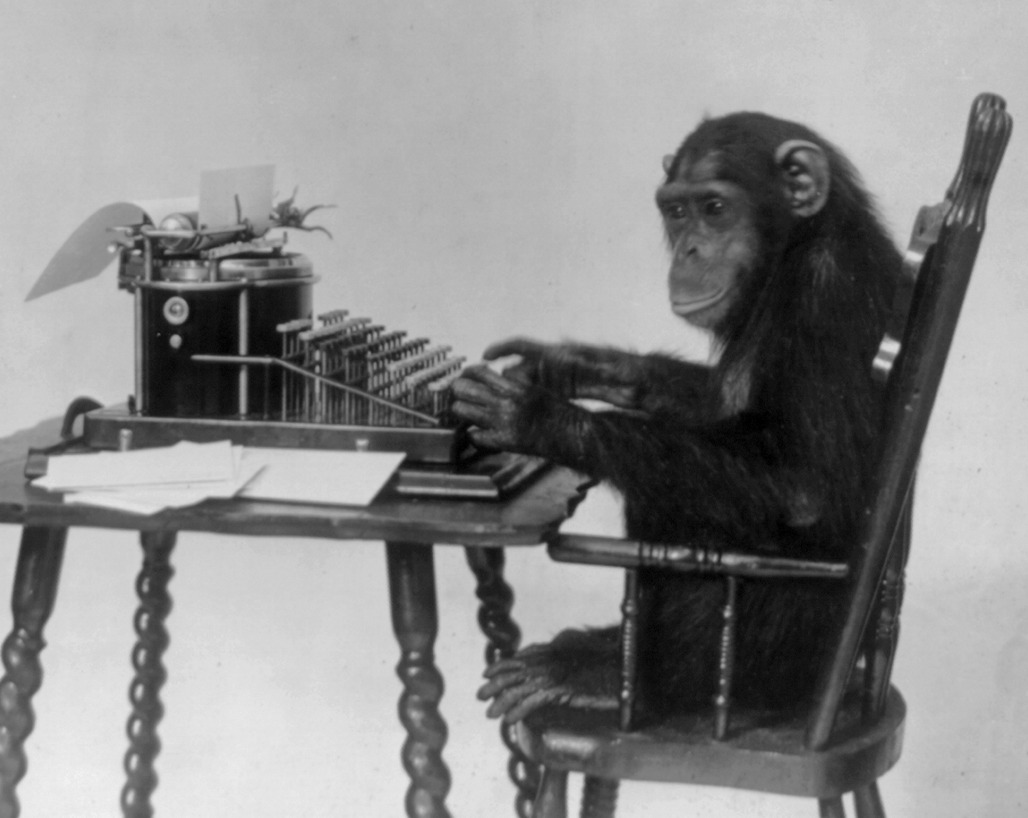
\includegraphics[width=0.25\textwidth]{figures/chimpanzee.jpg}
\captionof{figure}{Infinite monkey.}
\end{center}
\end{example}
\newpage 

\subsubsection{Kolmogorov's 0-1 Law}
We look at a generalisation of the Borel-Cantelli Lemma. To begin, let us define the notion of tail events and tail $\sigma$-algebra by first introducing some notations:
\begin{definition} \label{def:discrete_natural_filtration}
Let $(\Omega, \F, \p)$ be a probability space: 
\begin{enumerate}
    \item Let $\F_1, \F_2, ...$ be sub-$\sigma$-algebra of $\F$. Define the $\sigma$-algebra generated by their union:
    \begin{equation}
        \bigvee_{i=1}^n \F_i = \sigma\bracket{\bigcup_{i=1}^n \F_i},
    \end{equation}
    and extend this definition to the case when $n=\infty$.
    \item Let $\xi_1, \xi_2,...$ be a sequence of random variables defined on this probability space. Then
    \begin{equation}
        \sigma(\xi_1,\xi_2,...,\xi_n) = \bigvee_{i=1}^n \sigma(\xi_i),
    \end{equation}
    with this definition being extended to the infinite case.
\end{enumerate}
\end{definition}

\begin{definition}
Under the above settings, define $\F_n^p = \sigma (\xi_n, \dots, \xi_p)$ for $p\geq n$ and $\F_n^\infty = \sigma (\xi_n, \dots)$ (representing the future information), then the $\sigma-$ algebra associated with the sequence of random variables $\xi_1, \xi_2, ...$ is
\begin{equation*}
    \cT = \bigcap_{n=1}^\infty \F_n^\infty
\end{equation*}
is called the \textbf{tail $\sigma-$algebra}. Events of $\cT$ are called tail events.
\end{definition}

We are more interested in studying tail $\sigma$-algebra associated with a mutually independent sequence of random variables $\xi_1, \xi_2, ...$. If this assumption holds, then we have the following observation:
\begin{lemma}
For all $n \geq 2$, $\F_1^n$ and $\F_{n+1}^\infty$ are independent.
\end{lemma}

\begin{proof}
Recall the shortcut developed in lemma \ref{lem:independence_shortcut}! We first prove that $\F_1^n$ is independent with $\F_{n+1}^p$ for any $n+1 \leq p < \infty$. Note that $\F_1^n$ is generated by the $\pi$-system $\cup_{i=1}^n \sigma(\xi_i)$ and $\F_{n+1}^p$ is similarly generated by the $\pi$-system $\cup_{i=n+1}^p \sigma(\xi_i)$, and that these $\pi$-systems are independent, so we know that $\F_1^n$ is independent with $\F_{n+1}^p$ for any finite $p$. Now note that $\F_n^\infty$ is generated by the $\pi$-system $\cup_{p\geq n+1} \F_{n+1}^p$, so $\F_1^n$ is generated by $\F_{n+1}^\infty$.
\end{proof}

Note that $\cT \subseteq \F_n^\infty$ for any \textbf{finite} $n \geq 1$, so we have $\cT$ being independent with any $\F_1^n$. This provides an interpretation of the definition of a tail event $A \in \cT$, that \textit{its occurrence is independent of a finite number of changes in values of $\xi_n$}. An important example will be to note that the convergence of a sequence of random variable $\xi_1, \xi_2, ...$ is not affected when only a finite number of $\xi_n$'s are changed. 

\begin{example}
We see, for example, that $\set{\xi_{10} \in B}$ may not be in $\cT$, since its occurrence may be affected by changing a finite number of $\xi_n$, in our case being $\xi_{10}$. We also note that $\set{\omega \,|\, \forall n, \, \xi_n \notin \B}$ is not in $\cT$ since its occurrence may change by just affecting a value of $\xi_n$.
\end{example}

In fact, the above observations lead to a more surprising result! Since $\cup_{n\geq 1} \F_1^n$ is a $\pi$-system generating $\F_1^\infty$, we see that $\cT$ is independent with $\F_1^\infty$, and hence $\cT$ is actually independent with itself! This leads to the well-known Kolmogorov's Zero-One Law.

\begin{theorem}[Kolmogorov's Zero-One Law]
Let $\xi_1, \xi_2, \dots$ be a sequence of independent random variables, and let $A \in \cT$. Then $\p(A)$ can only have a value of zero or one.
\end{theorem}

\begin{proof}
We have $\p(A) = \p(A \cap A) = (\p(A))^2$, so $\p(A)$ must has value zero or one. 
\end{proof}

\begin{example}
Given independent sequence $\xi_1, \xi_2, ...$ and $B_1, B_2, ... \in \B(\R)$, then $\set{\xi_n \in B_n \text{ i.o.}} = \cap_{n=1}^\infty \cup_{k\geq n} \set{\xi_k \in B_k} \in \cT$. Now consider the independent events $A_1, A_2, ...$, then the sequence of random variables $\chi_{A_1}, \chi_{A_2}, ...$ are independent, and that the event $\limsup_{n} A_n := \set{\chi_{A_i} = 1 \text{ i.o.}}$ is a tail event associated with this independent sequence of random variables. The Kolmogorov's Zero-One Law then says that $\limsup_{n} A_n$ must have probability zero and one, which coincides with our observation from the Borel-Cantelli lemmas.
\end{example}

Perhaps the most important application of Kolmogorov's Zero-One Law is that it says that a random series of \textbf{independent} random variables must converge or diverge almost surely. Let $\xi_1, \xi_2, ...$ be sequence of independent random variables. Then obviously the following function is $\F_k^\infty$ measurable:
\begin{equation*}
    \limsup_{n\to\infty} \sum_{i\geq k} \xi_i, \quad \liminf_{n\to\infty} \sum_{i\geq k} \xi_i, \quad \lim_{n\to\infty} \sum_{i\geq k} \xi_i
\end{equation*}

As a result, the following functions are $\cT$ measurable:
\begin{equation*}
    \limsup_{n\to\infty} \sum_{i\geq 1} \xi_i, \quad \liminf_{n\to\infty} \sum_{i\geq 1} \xi_i, \quad \lim_{n\to\infty} \sum_{i\geq 1} \xi_i
\end{equation*}

In particular, the following set is a tail event associated with the given independent sequence of random variables:
\begin{equation*}
A = \set{\omega \, \bigg| \, \sum_{i\geq 1} \xi_i \text{ exists}},
\end{equation*}

and as a result of the Kolmogorov 0-1 law, we have the following 
\begin{corollary}
If $\xi_1, \xi_2, \dots$ is a sequence of independent random variables, then $\sum_{n=1}^\infty \xi_n$ either converges a.s. or diverges a.s.
\end{corollary}

We finally note an application of Kolmogorov 0-1 law:
\begin{example}
Let $\eta$ be a real-valued random variable that is measurable with respect to the $\sigma-$algebra $\cT$, i.e. $\{ \eta \in B\} \in \cT,$ $B \in \B(\R)$. Then $\eta$ is degenerate, i.e. there is a constant $c$ such that $\p(\eta = c) = 1$.
\end{example}

\begin{proof}
Note that for all $x \in \R$ one have $\p(\eta \leq x) \in \set{0,1}$ by the Kolmogorov 0-1 law. Take $c = \inf_{x \in \R \,|\, \p(\eta \leq x) = 1}$. Such an infinmum exists given that the distribution function is increasing, so if the infinmum does not exists then it means $0 = \p(\varnothing) = \p(\eta \leq -\infty) = 1$, which is a contradiction. It is easy to check that $\p(\eta = c) = 1$ by utilising the fact that $\p(\eta \leq x)$ is an increasing cadalag, and we will leave it as an exercise.
\end{proof}

There are many more zero-one laws in probability theory, but we will defer the discussion of those statements to a later chapter.
\newpage 

\subsection{More on Almost Sure Convergence}
\subsubsection{Almost sure convergence implies convergence in probability}
Recall the definition of almost sure convergence: a sequence $\xi_1, \xi_2, \dots$ of random variables converges almost surely to the random variable $\xi$ (denoted as $\xi_n \xrightarrow{a.s} \xi$) if $\p(\set{\omega \,|\, \xi_n(\omega) \not \to \xi(\omega)}) = 0$. This section is dedicated to explore the relationships between almost sure convergence, $L^p$ convergence and convergence in probability. As a warm up, we begin by the following equivalent definition of almost sure convergence.

\begin{proposition} \label{prop:as_prob_conv}
A necessary and sufficient condition that $\xi_n \to \xi$ $\p$-almost surely is that 
\begin{equation*}
    \p \bigg(\sup_{k \ge n} |\xi_k - \xi| \ge \varepsilon\bigg) \to 0, \quad n \to \infty,
\end{equation*}
    for every $\varepsilon > 0$.
\end{proposition}

\begin{hint}
The key step is to rewrite the set $\set{\xi_n \not\to \xi}$ into a countable union of sets. From the definition of convergence, we have
$$\xi_n(\omega) \not\to \xi(\omega) \iff \exists \, \epsilon > 0 \text{ s.t. } |\xi_n(\omega) - \xi(\omega)| \geq \epsilon \text{ infinitely often.}$$
So if we let $A_n^\varepsilon= \{ \omega: |\xi_n - \xi| \ge \varepsilon\}$ and $A^\varepsilon= \limsup A_n^\varepsilon= \{A_n^\varepsilon\, \text{ i.o.} \}$, then we have 
$$\{\omega \,|\, \xi_n(\omega) \not \to \xi(\omega) \} = \bigcup_{\varepsilon \ge 0} A^\varepsilon.$$
But this is not a countable union. Fortunately, the sets $A^\epsilon$ are nested, so one can restrict $\epsilon$ to the form $\epsilon = 1/m$ for some positive integers $m$, so we have
\begin{equation*}
\{\omega \,|\, \xi_n(\omega) \not \to \xi(\omega) \} =  \bigcup_{m=1}^\infty A^{1/m}.
\end{equation*}
The remaining of proof utilises the fact that the sets $A^\epsilon$ are nested.
\end{hint}

\begin{proof}
By nestedness of $A^\epsilon$ we have the following chain of implications:
\begin{align*}
    \p(\set{\omega: \xi_n \not \to \xi}) = 0 
    &\iff \p \bigg( \bigcup_{\varepsilon > 0} A^\varepsilon \bigg) = 0\\
    &\iff \p \bigg( \bigcup_{m=1}^\infty A^{1/m} \bigg) = 0\\
    &\overset{(*)}{\iff} \forall m \geq 1, \; \p(A^{1/m}) = 0\\
    &\iff \forall \varepsilon > 0, \; \p(A^\varepsilon) = 0
\end{align*}
The equivalence $(*)$ is justified below: first note that $\p(A^{1/m}) \leq \p(\cup_{m\geq 1} A^{1/m})$ so ($\Rightarrow$) clearly follows. The ($\Leftarrow$) direction follows from union bound: $\p(\cup_{m\geq 1} A^{1/m}) \leq \sum_{m\geq 1} \p(A^{1/m}) = 0$.\\

To complete the proof, we note that
\begin{equation*}
    \p(A^\varepsilon) = \p \bigg( \bigcap_{n \geq 1} \bigcup_{k \ge n} A_k^\varepsilon \bigg) = \lim_n \p \bigg( \bigcup_{k \ge n} A_k^\varepsilon \bigg) = \p\bigg(\sup_{k \ge n}|\xi_k - \xi| \ge \varepsilon \bigg),
\end{equation*}
so the result follows.
\end{proof}

From this equivalent statement, it is clear that almost sure convergence implies convergence in measure. In our summary diagram, we have proven the following highlighted implication.

\begin{figure} [H]
    \centering
    \begin{tikzcd}
    & \overset{L^p}{\to} \arrow[Rightarrow, d]  & \\
    \textcolor{red}{\overset{a.e.}{\to}} \arrow[Rightarrow, r, red] & \textcolor{red}{\overset{p}{\to} \arrow[Rightarrow, r]} & \overset{d}{\to}
\end{tikzcd}
\end{figure}

\begin{exercise}[Cauchy-like condition for almost sure convergence] \label{ex:as_Cauchy}
Show that the sequence $\{\xi_n\}_{n\geq 1}$ converges almost surely iff, for all $\varepsilon > 0$, 
\begin{equation*}
    \lim_{n\to\infty} \p \bigg(\sup_{k, l \ge n} |\xi_{k} - \xi_l| \ge \varepsilon\bigg) = 0,
\end{equation*}
or equivalently,
\begin{equation*}
    \p \bigg(\sup_{k \ge 0} |\xi_{n+k} - \xi_n| \ge \varepsilon\bigg) \to 0, \quad n \to \infty.
\end{equation*}
\end{exercise}

\begin{hint}
Let
\begin{equation*}
    B_{k,l}^\varepsilon = \{ \omega: |\xi_k - \xi_l| \ge \varepsilon\} , \quad B^\varepsilon = \bigcap_{n=1}^\infty \bigcup_{k, l \ge n} B_{k,l}^\varepsilon.
\end{equation*}
Then 
$$\{ \omega: \{\xi_n(\omega) \}_{n\ge1} \text{ is not convergent} \} = \bigcup_{\varepsilon > 0}B^\varepsilon,$$ 
and it can be shown as in proposition \ref{prop:as_prob_conv} that 
$$\p(\{ \omega: \{\xi_n(\omega) \}_{n\ge1} \text{ is not convergent} \}) = 0$$ 
if and only if the statement in the theorem holds.
\end{hint}

\subsubsection{Convergence in probability does not imply almost sure convergence}

The following counter-examples demonstrate that both convergences in probability and convergences in $L^p$ do not imply almost convergence. 

\begin{example}
Let $\xi_1, \dots, \xi_n$ be independent random variables on a certain probability space $(\Omega,\F,\p)$ taking value from $\set{0,1}$ with
\begin{equation*}
    \p(\xi_n = 1) = 1/n, \quad \p(\xi_n = 0) = 1 - 1/n.
\end{equation*}
We may choose $(\Omega,\F) = (\set{0,1}, \B(\set{0,1}))^{\N}$ and $\p$ being an appropriate infinite product measure. Then
\begin{equation*}
    \E[|\xi_n - 0|^p] = 1/n \to 0, \text{ so } \xi_n \xrightarrow{L^p} 0.
\end{equation*}
However, 
\begin{equation*}
    \{ \omega: \xi_n \to 0 \} = \{ \xi_n = 0 \text{ everywhere} \} = \bigcup_{n=1}^\infty \underbrace{\bigcap_{k \ge n} \{ \xi_k = 0 \}}_{\text{increasing sequence of sets}}
\end{equation*}
Therefore, 
\begin{align*}
    \p(\xi_n \to 0) &= \lim_{n \to \infty} \p \bigg(\bigcap_{k\ge n} \{ \xi_k = 0\} \bigg)\\
    &= \lim_{n \to \infty} \prod_{k \ge n} \p(\xi_k = 0)\\
    &= \lim_{n \to \infty} \prod_{k \ge n} \bigg(1 - \frac{1}{k}\bigg) = 0
\end{align*}
Indeed,
\begin{equation*}
    \prod_{k \ge n} \bigg( 1- \frac{1}{k} \bigg) = \lim_{N \to \infty} \prod_{k=n}^N \frac{k-1}{k} = \lim_{N \to \infty} \frac{n-1}{n} \frac{n}{n+1} \cdots \frac{N-1}{N} = 0.
\end{equation*}
Thus $\xi_n \not \xrightarrow{a.s.} 0$.
\end{example}

\begin{example}[Typewriter Sequence]
We provide another example on $([0,1], \B([0,1]), \Leb)$ with a similar flavor as the previous example. Consider the sequence 
\begin{equation}
f_n := \chi_{A_n}, \quad A_n = \sqbracket{\frac{n}{2^k} - 1, \frac{n+1}{2^k} - 1}
\end{equation}
whenever $k \geq 0$ and $2^k \leq n < 2^{k+1}$ The first few $A_n$ is as followed: 
$$[0,1], [0,1/2], [1/2, 1], [0,1/4], [1/4,1/2], [1/2,3/4], [3/4,1], ...$$
You can plot the indicator functions yourself, or look at some demonstrations on websites. \footnote{e.g. \url{https://math.stackexchange.com/questions/1412091/the-typewriter-sequence}}. You will see that the indicator functions move from left to right over $[0,1]$, then half its width and repeat again, which provides an explanation of the sequence's name.

\begin{center}
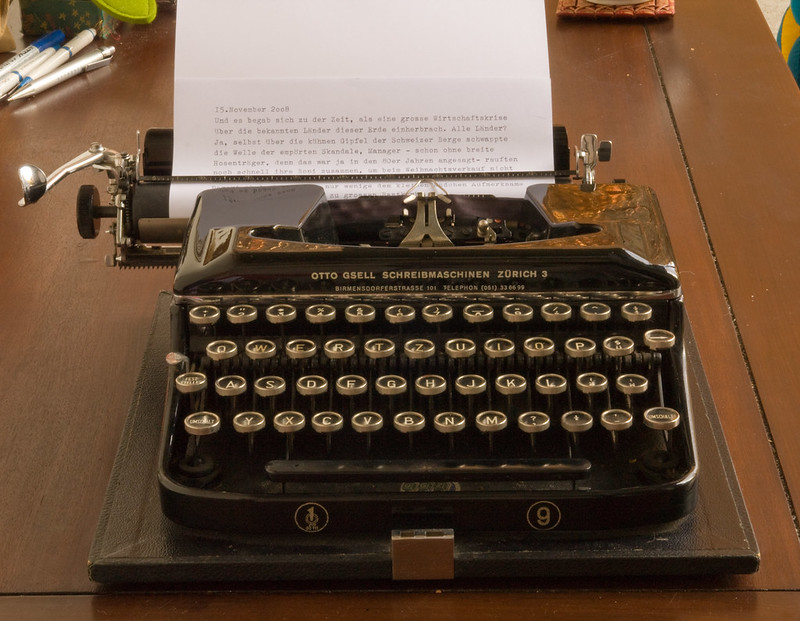
\includegraphics[width=0.4\textwidth]{figures/typewriter.jpg}
\captionof{figure}{A typewriter. Figure provided by Dr. Shordzi under the Creative Common 2.0 License: \url{https://creativecommons.org/licenses/by-sa/2.0/}}
\end{center}

The convergence in $L^p$ for any $p < \infty$ (hence convergence in $L^p$) of the sequence to zero is proven by noting that the width of indicator function vanishes as $n \to \infty$. However, given that the indicator function moves from left to right infinitely many times, for all $\omega \in [0,1]$, $f_n(\omega) = 1$ (and 0) infinitely often. As a result, $f_n(\omega)$ does not converge almost surely.
\end{example}

However, the implication from almost sure convergence to convergence in probability admits a partial converse: if a sequence converges in probability, then we can extract a subsequence that converges almost surely. To prove this important result, we note that 

\begin{lemma} \label{lem:as_conv_sufficient}
A sufficient condition for $\xi_n \xrightarrow{a.s.} \xi$ is that
\begin{equation*}
    \sum_{n=1}^\infty \p(|\xi_n - \xi| \ge \varepsilon) < \infty 
\end{equation*}
is satisfied for all $\varepsilon > 0$.
\end{lemma}

\begin{proof}
Denote the event $A_n^\varepsilon = \{\omega \,|\, |\xi_n(\omega) - \xi(\omega)| \ge \varepsilon\}$ as required. Since $\sum_{k\geq 1} \p(A^\epsilon) < \infty$, by first Borel-Cantelli lemma we know that $\p(A^\varepsilon) := \p(A_n^\epsilon \; \text{i.o.}) = 0$. Following the arguments in proposition \ref{prop:as_prob_conv} we know that $\p(\set{\omega \,|\,\ \xi_n \not\to \xi}) = 0$ as desired.
\end{proof}

\begin{corollary} \label{cor:as_conv_sum_sufficient}
Let $(\varepsilon_n)_{n\ge 1}$ be a sequence of positive numbers such that $\varepsilon_n \downarrow 0$ as $n \to \infty$. Then if $\xi_n$ converges to $\xi$ in probability sufficiently fast in the sense that 
\begin{equation*}
    \sum_{n=1}^\infty \p(|\xi_n - \xi| \ge \varepsilon_n) < \infty,
\end{equation*}
then $\xi_n \xrightarrow{a.s.} \xi$.
\end{corollary}

\begin{proof}
Fix an arbitrary $\epsilon > 0$. Choose $N$ such that for all $n \geq N$ we have $\epsilon_n < \epsilon$. Then 
\begin{equation*}
    \sum_{n=1}^\infty \p(|\xi_n - \xi| \geq \epsilon) \leq \underbrace{\sum_{n=1}^{N-1} \p(|\xi_n - \xi| \geq \epsilon)}_{\leq N-1 < \infty} + \underbrace{\sum_{n=N}^\infty \p(|\xi_n - \xi| \geq \epsilon)}_{<\infty},
\end{equation*}
hence by the above lemma \ref{lem:as_conv_sufficient} we have $\xi_n \overset{\text{a.s.}}{\to} \xi$ as $n \to \infty$.
\end{proof}

We may now prove our key result for this subsection.
\begin{theorem} \label{thm:subsequence_conv_prob}
If $\xi_n \xrightarrow{p} \xi$, then there exists a subsequence such that
\begin{equation*}
    \xi_{n_k}\xrightarrow{a.s.} \xi.
\end{equation*}
\end{theorem}

\begin{proof}
Since $\lim_{n \to \infty} \p(|\xi_n - \xi| > 1/k) = 0$ for all $k \ge 1$, we can choose a subsequence such that 
\begin{equation*}
    \p (|\xi_n - \xi| > k^{-1}) \le 2^{-k} \quad \forall k \ge 1
\end{equation*}
Since $\sum_{k=1}^\infty 2^{-k}$ converges, by above corollary \ref{cor:as_conv_sum_sufficient} we have $\xi_{n_k}\xrightarrow{a.s.} \xi$.
\end{proof}

The trick of extracting a almost surely convergent subsequence is very helpful in justifying limits. Here is an immediate application of the above theorem:
\begin{corollary}
If $\xi_1 \ge \xi_2 \ge \cdots \ge 0$, are random variables and $\xi_n \xrightarrow{p} 0$, then
\begin{equation*}
    \xi_n \xrightarrow{a.s.} 0.
\end{equation*}
\end{corollary}

\begin{proof}
Note that $\xi_n \xrightarrow{a.s} 0 $ if and only if $\limsup \xi_n = 0$ a.s. Let $\varepsilon > 0$. Denote $A_n = \{\xi_n > \varepsilon \}$. Then by continuity,
\begin{equation*}
    \p(\limsup \xi_n > \varepsilon) = \p(\xi_n > \varepsilon \, i.o.) = \lim_{n \to \infty} \p\bigg(\bigcup_{k \ge n} A_k\bigg).
\end{equation*}
Since $A_n$ is non-increasing, the right hand side equals $\lim_{n \to \infty} \p(A_n)$ which is $0$ since $\xi_n \xrightarrow{p} 0$. Thus 
\begin{equation*}
    \p(\limsup \xi_n > \varepsilon) = 0 \quad \forall \varepsilon > 0,
\end{equation*}
and therefore
\begin{equation*}
    \p(\xi_n \not \to \xi) \le \sum_{m=1}^\infty \p(\limsup \xi_n > 1/m) = 0.
\end{equation*}
\end{proof}

\begin{unexaminable}
We finally note an observation regarding convergence in probability:
\begin{corollary}
Let $\xi, (\xi_n)_{n\geq 1}$ be random variables on the probability space $(\Omega,\F,\p)$. Then $\xi_n \to \xi$ in probability as $n \to \infty$ iff for any subsequence, there is a further subsequence that converges $\p$-a.s. to $\xi$.
\end{corollary}
\begin{proof}
The $(\Rightarrow)$ direction is proven in theorem \ref{thm:subsequence_conv_prob}. For $(\Leftarrow)$, we note that almost sure convergence implies convergence in probability. We also recall a basic fact that in metric space, if $(a_m)$ is a sequence such that for any subsequence there is a further subsequence that converges to some element $a$, then $a_m \to a$. Since convergence in probability is metrisable as shown in exercise \ref{ex:metric_for_conv_in_prob}, we may directly use this result to complete the proof.
\end{proof}
\end{unexaminable}

\begin{exercise}
\begin{enumerate}
    \item[]
    \item Let $\xi_1, \xi_2, \dots, \xi_n$ be i.i.d. random variables with the standard exponential distribution and define
    \begin{equation*}
        M_n = \max \{\xi_1, \dots, \xi_n \}.
    \end{equation*}
    Show that as $n \to \infty$
    \begin{itemize}
        \item $\limsup \xi_n/\log{n} = 1$ a.s.
        \item $M_n / \log{n} = 1$ a.s.
    \end{itemize}
\end{enumerate}
\end{exercise}

\subsubsection{Almost sure convergence and $L^p$ convergence}
It has been proven in elementary measure theory classes that having almost sure convergence does not guarantee $L^p$ convergence. Here we prove a result which states that if we have almost sure convergence and convergence in mean, then we have $L^1$ convergence.
\begin{theorem}
Let $\xi_n$ be a sequence of nonnegative random variables such that $\xi_n \xrightarrow{a.s.} \xi$ and $\E[\xi_n] \to \E[\xi] < \infty$. Then $\xi_n \xrightarrow{L^1} \xi$, or 
\begin{equation*}
    \E[|\xi_n - \xi|] \to 0, \quad n\to \infty.
\end{equation*}
\end{theorem}

\begin{proof}
We have $\E[|\xi_n|] < \infty$ for sufficiently large $n$ and therefore for such $n$ we have
\begin{align*}
    \E[|\xi_n - \xi|] &= \E[\xi - \xi_n]\chi_{\xi \ge \xi_n} + \E[\xi_n - \xi]\chi_{\xi_n \ge \xi}\\
    &= 2 \E[\xi - \xi_n]\chi_{\xi \ge \xi_n} + \E[\xi_n - \xi].
\end{align*}
But $0 \le (\xi - \xi_n) \chi_{\xi \ge \xi_n} \le \xi$. Therefore, by the dominated convergence theorem, $\E[\xi-\xi_n] \chi_{\xi \ge \xi_n} \to 0$.
\end{proof}

\begin{unexaminable}
\begin{remark}
More generally, if we know that a uniformly integrable sequence of random variables converges in almost surely, then it converges in $L^1$ as well. This follows from Vitali convergence theorem, and that an almost-surely converging sequences must converge in probability. (Proposition \ref{prop:as_prob_conv})
\end{remark}
\end{unexaminable}

\subsection{Strong Law of Large Numbers}
We are now ready to prove some strong law of large numbers. A strong law of large number is the statement of the following form: given $\xi_1, \xi_2, \dots$ is a sequence of integrable random variables, which is assumed to be independent (or "weakly correlated"). Let $S_n = \xi_1 + \xi_2 + ... + \xi_n$, then the sequence $(\xi_n)_{n\geq 1}$ is said to satisfy the strong law of large numbers if 
\begin{equation*}
    \frac{S_n - \E[S_n]}{n} \xrightarrow{\text{a.s.}} 0.
\end{equation*}
It is stronger than the weak law of large number as proven in chapter 4 in the sense that we only have convergence in probability in contrast to almost sure convergence. \\

Recall that for i.i.d. $\xi_n$ with a second moment assumption (i.e. $\V[\xi_1] < \infty$) we have the $L^2$ weak law of large number. If we impose an excessive moment assumptions, we can prove a strong law of large number.

\begin{proposition}[Cantelli's Strong Law of Large Numbers]
Let $\xi_1, \xi_2, \dots$ be i.i.d. random variables with $\E[\xi_1^4] < \infty$. Then
\begin{equation}
    \frac{S_n - \E[S_n]}{n} \xrightarrow{\text{a.s.}} 0,
\end{equation}
i.e. $\{ \xi_n \}$ satisfies the strong law of large numbers.
\end{proposition}

\begin{hint}
Without loss of generality we centralise the random variables by substracting its mean, then $\E[\xi_1] = \E[\xi_1^3] = 0$. Fix an arbitrary $\epsilon > 0$, we hope to use lemma \ref{lem:as_conv_sufficient} to establish almost sure convergence. We will bound the probability $\p(|S_n/n| \geq \epsilon) = \p(|S_n| \geq n\epsilon)$ by using Chebyshev inequality.
\end{hint}

\begin{proof}
Let us therefore bound the probability $\p(|S_n/n| \geq \epsilon)$, so that it decays fast enough and $\sum_{n\geq 1} \p(|S_n/n|\geq \epsilon) < \infty$. We might therefore want $\p(|S_n|\geq n\epsilon) = O(1/n^2)$. \\

To use the Chebyshev inequality, one has to bound the $k$-th moment of $S_n/n$ (where $k$ is an even number). We want the $k$-th moment to be of order $O(1/n^2)$. We may look at second moments:
\begin{equation}
\V[S_n/n] = n\E[\xi_1]/n^2,
\end{equation}
which is not enough for Chebyshev inequality. We have to look at the forth moments. In the expansion of forth moments, the only non-vanishing terms are terms of the form $\E[\xi_j^4]$ and $\E[\xi_i^2 \xi_j^2] = \E[\xi_i^2] \E[\xi_j^2]$ with $i \neq j$, noticing that the odd moments of $\xi_i$ vanishes. We therefore have the expansion
\begin{equation}
\E[S_n^4] = \E\sqbracket{\sum_{k=1}^n \xi_k^4 + {4 \choose 2, 2} \sum_{j,k=1, j < k} \xi_j^2 \xi_k^2}
\end{equation}
where ${4 \choose 2,2} = 4!/(2!)^2 = 6$ comes from the multinomial theorem. Now notice that there are $n(n-1)/2$ unique ways to choose the indices $(j,k)$ such that $j < k$, therefore we have, from the i.i.d. assumption,
\begin{equation}
\E[|S_n/n|^4] = \frac{1}{n^4} \bracket{n\E[\xi_1^4] + 3n(n-1) (\E[\xi_1^2])^2}
\end{equation}
Finally, note from Lyapunov inequality (corollary \ref{cor:lyapunov_ineq}) that $\E[\xi_1^2]^{1/2} \leq \E[\xi_1^4]^{1/4}$, so we have 
\begin{equation}
\E[|S_n/n|^4] \leq \frac{3n^2 - 2n}{n^4}\E[\xi_1^4] \lesssim \frac{1}{n^2},
\end{equation}
and therefore $\sum_{n\geq 1} \p(|S_n/n|\geq \epsilon) \lesssim \sum_{n\geq 1} n^{-2} < \infty$ as desired.
\end{proof}

This strong law of large number is already very useful for practical purposes. It can be used when $\xi_1$ follows common distributions (e.g. Normal, Gamma, Binomial, ...), or have finite supports. However, as seen below, we can impose much weaker assumptions on the moments of $\xi_i$. \\

We will follow Kolmogorov's approaches in proving his strong law of large numbers. The approach is cumbersome since it involves many technical lemma in analysis, nevertheless it opens up routes of proving more general statements about convergence of random series. Another route is to consider truncation of random variables, which is simpler and actually leads to a stronger version of strong law of large number by Etemadi as proved in \cite{EtemadiSLLN}. We will not cover this proof in our notes. \\

Back to Kolmogorov's approach. Let us start with the following Kolmogorov maximal inequality:

\begin{proposition}[Kolmogorov's maximal inequality]
Let $\xi_1, \xi_2, \dots$ be independent random variables with finite variances. Then $\forall n \ge 1$ and $x > 0$, we have 
\begin{equation*}
    \p\bracket{\max_{1 \le k \le n} | S_k - \E[S_k]| \ge x} \le \frac{\V[S_n]}{x^2}.
\end{equation*}
\end{proposition}

Notice that this is a stronger version of the Chebyshev inequality, since Chebyshev inequality only gives
\begin{equation*}
    \p\bracket{|S_k - \E[S_k]| \geq x} \leq \frac{\V[S_n]}{x^2}.
\end{equation*}

Combining with union bound we get
\begin{equation*}
    \p\bracket{\max_{1\leq k \leq n} |S_k - \E[S_k]| \geq x} = \p\bracket{\bigcup_{k=1}^n \set{|S_k - \E[S_k]| \geq x}} \leq \frac{\textcolor{blue}{n}\V[S_n]}{x^2}.
\end{equation*}

What this maximal inequality does is to remove the factor of $n$ generated in the union bound. As seen in \ref{lem:as_conv_sufficient}, if we are able to bound the probability of maximum deviation using maximal inequalities, then we can use Borel-Cantelli to establish almost sure convergence.

\begin{hint}
Again we subtract the random variables with its mean to set $\E[\xi_1] = 0$. The key step is to note that the events $A_k, k=1,...,n$ is a partition of $A = \set{\omega\,|\, \max_{1\leq k \leq n} |S_k(\omega)| \geq x}$, where $|S_j|$ first exceeds $x$ at $j=k$, i.e.
\begin{equation*}
    A_k := \set{\omega \,|\, |S_j(\omega)| < x \text{ and } |S_k(\omega)| \geq x}.
\end{equation*}
Now show that $\E[S_n^2 \chi_{A_k}] \geq x^2 \p(A_k)$ by breaking up $S_n$.
\end{hint}

\begin{proof}
From the above hint, we have
\begin{equation*}
    \V[S_n^2] \geq \E[S_n^2 \chi_A] = \sum_{k=1}^n \E[S_n^2 \chi_{A_k}].
\end{equation*}
But 
\begin{align*}
    \E[S_n^2 \chi_{A_k}] &= \E[(S_k + \xi_{k+1} + ... + \xi_n)^2 \chi_{A_k}] \\
    &= \underbrace{\E[S_k^2 \chi_{A_k}]}_{\geq x^2 \p(A_k)} + \underbrace{2\E[(S_k \chi_{A_k})(\xi_{k+1} + ... + \xi_n)]}_{= 2\E[S_k \chi_{A_k}] \E[\xi_{k+1} + ... + \xi_n] = 0} + \underbrace{\E[(\xi_{k+1} + ... + \xi_n)^2]}_{\geq 0} \\
    &\geq x^2 \p(A_k),
\end{align*}
so we have
\begin{equation}
    \V[S_n^2] \geq x^2 \sum_{k=1}^n \p(A_k) = x^2 \p(A).
\end{equation}
\end{proof}

With this maximal inequality, we may prove the Kolmogorov's three series theorem, which states that the almost sure convergence of a (truncated) random series depends on the convergence of three deterministic series. Here we will prove the statement in three steps:

\begin{lemma}[Three-series theorem, part I] \label{lem:three_series_1}
Suppose $\xi_1, \xi_2, ...$ are independent real-valued series and have $\E[\xi_i] = 0$ for all $i$. If we know that $\sum_{i\geq 1} \V[\xi_i] < \infty$, then $\sum_{i\geq 1} \xi_i$ converges almost surely.
\end{lemma}

\begin{proof}
Since we are not given the limit for which the random series converges, the best way of proving this theorem is to resort on proving the series $S_n := \sum_{i=1}^n \xi_i$ being Cauchy as in exercise \ref{ex:as_Cauchy}. To this we need to show that as $n \to \infty$,
\begin{equation*}
    \p\bracket{\sup_{k\geq 1} |S_{n+k} - S_k| \geq \epsilon} \to 0
\end{equation*}
We note that for all $m < \infty$ we have, from the above maximal inequality,
\begin{equation}
    \p\bracket{\sup_{1 \leq k \leq m} |S_{n+k} - S_k| \geq \epsilon} \leq \epsilon^{-2} \sum_{k=1}^m \V[\xi_{n+k}] \leq \epsilon^{-2} \sum_{k=1}^\infty \V[\xi_{n+k}],
\end{equation}
so one can send $m \to \infty$ (by continuity from below):
\begin{equation}
\p\bracket{\sup_{k \geq 1} |S_{n+k} - S_k| \geq \epsilon} \leq \sum_{k=1}^\infty \V[\xi_{n+k}] \overset{n \to \infty}{\to} 0
\end{equation}
as desired, so the series $S_n$ converges almost surely.
\end{proof}

\begin{theorem}[Three-series theorem, part II] \label{thm:three_series_2}
Let $\xi_1, \xi_2, \dots$ be independent random variables. If $\sum_{n=1}^\infty \E[\xi_n]$ and $\sum_{n=1}^\infty \V[\xi_n]$ converge, then $\sum_{n=1}^\infty \xi_n$ converges a.s.
\end{theorem}

\begin{proof}
This follows by breaking the random series into two parts:
\begin{equation}
\sum_{i=1}^\infty \xi_i = \sum_{i=1}^\infty (\xi_i - \E[\xi_i]) + \sum_{i=1}^\infty \E[\xi_i],
\end{equation}
provided that the two series in the RHS actually converge, so the theorem follows.
\end{proof}

\begin{unexaminable}
The above thre-series theorem is enough for our application, but for completion let us state the full Kolmogorov's three-series theorem:
\begin{corollary}[Three-series theorem, part III] \label{cor:three_series_3}
Let $\xi_1, \xi_2, ...$ be independent random variables. Let further $A>0$ be \textbf{some} constant, and $\eta_i = \xi_i \chi_{|\xi_i| \leq A}$ be the truncated random variables. Then $\sum_{i\geq 1} \xi_i$ converges almost surely if and only if the following three series converge:
\begin{center}
(1) $\sum_{i\geq 1} \p(|\xi_i| > A)$, (2) $\sum_{i\geq 1} \E[\eta_i]$ and (3) $\sum_{i\geq 1} \V[\eta_i]$
\end{center}
When $A = \infty$ this theorem reduces to part II. Moreover, when $\sum_{n=1}^\infty \xi_n$ converges a.s., then for all $A>0$ the conditions (1)-(3) holds.
\end{corollary}

\begin{proof}
(Sufficiency). Notice that part II guarantees that $\sum_{i\geq 1} \eta_i$ converges almost surely, and the convergence of $\sum_{i\geq 1} \p(|\xi_i| > A)$ means that $\p(|\xi_i| > A \text{ i.o.}) = 0$ by the first Borel-Cantelli lemma. Therefore, almost surely $\xi_i = \eta_i$ eventually, and in such case $\sum_{i\geq 1} \xi_i$ converges. \\

(Necessity). We prove that a.s. convergence $\implies$ (1) $\implies$ (3) $\implies$ (2). Proving the first implication is simple: provided that $\xi_i$ are independent, we know from the second Borel-Cantelli lemma that if (1) does not hold then $\p(|\xi_i|>A \text{ i.o.}) = 1$, and that $\lim_{n\to\infty} \sum_{i=1}^n \xi_i$ may not exist.\\

We now prove (1) $\implies$ (3) by assuming (1) is true but (3) is false for contradiction, then by exercise \ref{ex:Lindeberg_for_bounded_rv}, we know that
\begin{equation*}
    \frac{\tilde{S}_n - \E[\tilde{S}_n]}{D_n} \xrightarrow{d} \mathsf{N}(0,1), \quad \tilde{S}_n = \sum_{i=1}^n \E[\eta_i], \; D_n = \sum_{i=1}^n \V[\eta_i].
\end{equation*}
Now since $\sum_{i\geq 1} \xi_i$ converges almost surely, so is $\sum_{i\geq 1} \eta_i$, so by sequencing the sequence $T_n = (\sum_{i=1}^n \eta_i) / D_n \overset{n\to\infty}\to 0$ almost surely (hence also in probability). Therefore, by Slutsky's theorem (proposition \ref{prop:addition_of_weak_limits}) we know that $S_n - T_n \xrightarrow{d} \mathsf{N}(0,1)$. But $S_n - T_n = -\bracket{\sum_{i=1}^n \E[\eta_i]}/D_n$, which is not random. We have a contradiction, so (1) $\implies$ (3). \\

We finally prove that (1) and (3) $\implies$ (2). This follows from part I of the three series theorem (lemma \ref{lem:three_series_1}), that $\lim_{n\to\infty} \sum_{i=1}^n (\eta_i - \E[\eta_i])$ exists. Provided that $\lim_{n\to\infty} \sum_{i=1}^n \eta_i$ exists as well, we know that (2) holds.
\end{proof}
\end{unexaminable}

We are now halfway through proving Kolmogorov's strong law of large numbers. To complete the proof we have to prove a few technical lemmas concerning the convergence of the weighted mean of the first terms of a converging sequence. You should be able to prove the following lemmas yourself using tools from elementary analysis classes.

\begin{lemma}[Toeplitz] \label{lem:Toeplitz}
Let $\{a_n\}$ be a sequence of nonnegative numbers, $b_n = \sum_{i=1}^n a_i$, $b_1 = a_1 > 0$, and $b_n \uparrow \infty, n \to \infty$. Let $\{ x_n \}_{n \ge 1}$ be a sequence of numbers converging to $x$. Then
\begin{equation*}
    \frac{1}{b_n} \sum_{j=1}^n a_j x_j \to x.
\end{equation*}
In particular, if $a_n = 1$, then
\begin{equation*}
    \frac{x_1 + \cdots + x_n}{n} \to x.
\end{equation*}
\end{lemma}

\begin{hint}
Observe that for all $1 \leq N \leq n$,
\begin{equation*}
\abs{\frac{1}{b_n}\sum_{j=1}^n a_j x_j - x} = \abs{\frac{1}{b_n}\sum_{j=1}^n a_j(x_j - x)} \leq \abs{\frac{1}{b_n}\sum_{j=1}^N a_j(x_j - x)} + \abs{\frac{1}{b_n}\sum_{j=N+1}^n a_j(x_j - x).}
\end{equation*}
Now choose $N$ such that $|x_j - x|$ is sufficiently small. Show that the tail (second term of RHS) is very small. Can you complete the proof from here?
\end{hint}

\begin{proof}
Fix $\epsilon > 0$. Choose $N_0 := N_0(\epsilon)$ such that for all $n \geq N_0$ we have $|x_j - x| < \epsilon/2$. Now choose $N_1 > N_0$ (which depends on $N_0$) such that $b_{N_1}^{-1} \sum_{j=1}^{N_0} |x_j - x| < \epsilon/2$, which exists since $|x_j - x|$ is bounded for $j = 1,...,N_0$. Then for any $n > N_1$, we have
\begin{align*}
\abs{\frac{1}{b_n}\sum_{j=1}^n a_j x_j - x} &\leq \abs{\frac{1}{b_n}\sum_{j=1}^{N_0} a_j(x_j - x)} + \abs{\frac{1}{b_n}\sum_{j=N+1}^n a_j(x_j - x)} \\
&\leq \frac{1}{b_{N_1}} \abs{\sum_{j=1}^N a_j(x_j - x)} + \abs{\frac{1}{b_n}\sum_{j={N_0}+1}^n a_j(x_j - x)}\\
&< \frac{\epsilon}{2} + \frac{\epsilon}{2} \underbrace{\bracket{\frac{1}{b_n} \sum_{j=N_0+1}^n a_j}}_{\leq 1} \leq \epsilon,
\end{align*}
so we have the above convergence.
\end{proof}

Here we give an application of the Toeplitz lemma by the following exercise:
\begin{exercise}
Suppose $(\xi_i)_{i\geq 1}$ is a sequence of independent random variables with common mean $m$ and variance $\V[\xi_k] = k\eta(k)$ with the condition that $\V[\xi_k] \to \infty$, but $\eta(k) > 0$ and $\eta(k) \searrow 0$ as $k \to \infty$. Use Toeplitz lemma to prove that the sequence satisfies weak law of large number, that $n^{-1} \sum_{i=1}^n \xi_i \to m$ as $n \to \infty$ in $L^2$ and in probability.
\end{exercise}

We then prove the Kronecker lemma.
\begin{lemma}[Kronecker]
Let $b_n$ be a sequence of positive increasing numbers, $b_n \uparrow \infty$ as $n \to \infty$ and let $\{x_n\}$ be a sequence of numbers such that $\sum x_n$ converges. Then 
\begin{equation*}
    \frac{1}{b_n}\sum_{j=1}^n b_j x_j \to 0, \quad n \to \infty.
\end{equation*}
In particular, if $b_n = n$, $x_n = y_n/n$ and $\sum y_n/n$ converges, then 
\begin{equation*}
    \frac{y_1 + \cdots + y_n}{n} \to 0, \quad n \to \infty.
\end{equation*}
\end{lemma}

\begin{hint}
We let $b_0 = S_0 = 0, S_n = \sum_{j=1}^n x_j$. In addition (for simplicity notations) we let $a_n$ as in Toeplitz lemma (lemma \ref{lem:Toeplitz}), such that $a_1 = b_1$ and $a_n = b_n - b_{n-1}$ for $n \geq 2$. The hint is to note Abel's summation formula:
\begin{align*}
    \sum_{j=1}^n b_j x_j = \sum_{j=1}^n b_j (S_j - S_{j-1}) &= b_n S_n - b_0 S_0 - \sum_{j=1}^n S_j (b_j - b_{j-1}) \\
    &= b_n S_n - b_0 S_0 - \sum_{j=1}^n a_j S_j.
\end{align*}
Can you draw parallels between the above formula and integration by parts?
\end{hint}

\begin{proof}
Dividing $b_n$ yields:
\begin{equation}
    \frac{1}{b_n} \sum_{j=1}^n b_j x_j = S_n - \underbrace{\frac{b_0 S_0}{b_n}}_{\to 0} - \frac{1}{b_n} \sum_{j=1}^n a_j S_j.
\end{equation}
So when $n\to \infty$, we see that $b_n^{-1} \sum_{j=1}^n b_j x_j \overset{n\to\infty}{\to} 0$ by Toeplitz lemma.
\end{proof}

With this, we may prove Kolmogorov's lemma, which laid a foundation for some of the most important theorems relating to the almost sure convergence of random series.

\begin{theorem}[Kolmogorov]
Let $\xi_1, \xi_2,\dots$ be a sequence of independent random
variables with finite second moments, and let there be positive numbers $b_n$ such that $b_n \nearrow \infty$ and 
\begin{equation*}
    \sum_{n\geq 1} \frac{\V[\xi_n]}{b_n^2} < \infty.
\end{equation*}
Then 
\begin{equation*}
    \frac{S_n - \E[S_n]}{b_n} \xrightarrow{a.s.} 0.
\end{equation*}
In the case where $b_n = n$, this is a strong law of large numbers.
\end{theorem}

\begin{hint}
Observe that 
\begin{equation*}
\frac{S_n - \E[S_n]}{b_n} = \frac{1}{b_n} \sum_{i=1}^n b_k \frac{\xi_k - \E[\xi_k]}{b_k}
\end{equation*}
and use Kronecker lemma to conclude.
\end{hint}

\begin{proof}
Note that 
\begin{equation*}
\sum_{k\geq 1} \V\sqbracket{\frac{\xi_k - \E[\xi_k]}{b_k}} = \sum_{k\geq 1} \frac{\V[\xi_k]}{b_k^2} < \infty,
\end{equation*}
so by part II of Kolmogorov's three series theorem (theorem \ref{thm:three_series_2}) the sum $\sum_{k\geq 1} (\xi_k - \E[\xi_k])/b_k$ converges almost surely, and by Toeplitz theorem applied on this series the desired result holds.
\end{proof}

In the case where the variables $\xi_1, \xi_2, \dots$ are not only independent but also identically distributed, we can obtain a strong law of large numbers without requiring (as in the theorem above) the existence of the second moment, provided that the first absolute moment exists.
\begin{theorem}[Kolmogorov's Strong Law of Large Numbers]
Let $\xi_1, \xi_2, \dots$ be a sequence of independent identically distributed random variables with $\E[|\xi_1|]<\infty$. Then
\begin{equation*}
    \frac{S_n}{n} \xrightarrow{n\to\infty} m =: \E[\xi_1], n \to \infty.
\end{equation*}
\end{theorem}

\begin{proof}
We first recall the relationship between tail probabilities and expectation (see \eqref{eq:exp_tail}): if $\xi\geq 0$ is an integrable random variable, then
\begin{equation}
    \E[\xi] = \int_{[0,\infty)}\p(\xi \ge x) \, \d x.
\end{equation}
As a result, it is not hard to see that the following inequality holds:
\begin{equation}
\sum_{n\geq 1} \p(\xi \geq n) \leq \E[\xi] \leq 1+\sum_{n\geq 1} \p(\xi \geq n),
\end{equation}
and hence $\sum_{n\geq 1} \p(|\xi| \geq n) \leq \E[|\xi|] < \infty$. By first Borel-Cantelli lemma, we know that $\p(|\xi_n| \geq n \text{ i.o.}) = 0$, i.e. $|\xi_n|< n$ eventually, $\p$-almost everywhere. So by constructing truncated random variables $\tilde{\xi}_n = \xi_n\chi_{|\xi_n| < n}$, we have 
\begin{equation*}
    \frac{S_n}{n} \xrightarrow{n\to\infty} 0 \text{ a.s.} \iff \frac{1}{n} \sum_{i=1}^n \tilde{\xi}_i \xrightarrow{n\to\infty} 0 \text{ a.s.}
\end{equation*}
Note that by dominated convergence theorem, $\E[\tilde{\xi}_n] \xrightarrow{n\to\infty} \E[\xi_1] = 0$; so by Toeplitz lemma (lemma \ref{lem:Toeplitz}) we have $n^{-1} \sum_{i=1^n} \E[\tilde{\xi}_i] \overset{n\to\infty}{\to} 0$. Therefore
\begin{equation*}
    \frac{S_n}{n} \xrightarrow{n\to\infty} 0 \text{ a.s.} \iff \frac{1}{n} \sum_{i=1}^n (\tilde{\xi}_i - \E[\tilde{\xi}_i]) \xrightarrow{n\to\infty} 0 \text{ a.s.}
\end{equation*}
But we note that 
\begin{align*}
    \V\sqbracket{\sum_{n\geq 1} \frac{\tilde{\xi}_n - \E[\tilde{\xi}_n]}{n}} \leq  \sum_{n=1}^\infty \frac{\E[\xi_1^2 \chi_{|\xi_1| < n}]}{n^2}
    &= \sum_{n=1}^\infty \frac{1}{n^2} \sum_{k=1}^n \E[\xi_n^2 \chi_{\set{|\xi_1| \in [k-1,k)}}] \\
    &= \sum_{k=1}^\infty \E[\xi_n^2 \chi_{|\xi_1| \in [k-1,k)}] \underbrace{\bracket{\sum_{n=k}^\infty \frac{1}{n^2}}}_{\leq 2/k} \\
    &= 2\sum_{k=1}^\infty \E\bracket{|\xi| \underbrace{\frac{|\xi|}{k}}_{\leq 1} \chi_{\set{|\xi_1| \in [k-1,k)}}} \leq 2\E[|\xi_1|] < \infty,
\end{align*}
so by three series theorem we know that $n^{-1} \sum_{i=1}^n (\tilde{\xi}_i - \E[\tilde{\xi}_i]) \overset{n\to\infty}\to 0$ $\p$-a.s, which completes the proof.
\end{proof}

\begin{remark}
The theorem admits a converse in the following sense. Let $\xi_1, \xi_2, \dots$ be a sequence of independent identically distributed random variables such that
\begin{equation*}
    \frac{\xi_1 + \cdots + \xi_n}{n} \to C < \infty,
\end{equation*}
with probability $1$. Then $\E[|\xi_1|] < \infty$ and $C = \E[\xi_1]$. In fact, if $S_n/n \xrightarrow{a.s.}  C$, then
\begin{equation*}
    \frac{\xi_n}{n} = \frac{S_n}{n} - \bigg( \frac{n-1}{n}\bigg) \frac{S_{n-1}}{n-1} \xrightarrow{a.s.} 0
\end{equation*}
and therefore $\p(|\xi_n| > n \, \, i.o.) = 0$. By the Borel-Cantelli lemma
\begin{equation*}
    \sum \p(|\xi_1| > n) < \infty,
\end{equation*}
and using one of our lemmas above, we have $\E[|\xi_1|] < \infty$. It then follows from the theorem that $C = \E[\xi_1]$. Consequently, for independent identically distributed random variables, the condition $\E[|\xi_1|] < \infty$ is necessary and sufficient for the convergence (with probability 1) of the ratio $S_n/n$ to a finite limit.
\end{remark}

% \begin{remark}
% We can write
% \begin{equation*}
%     \frac{S_n}{n} \xrightarrow{a.s.} m
% \end{equation*}
% as 
% \begin{equation*}
%     \sum_{k=1}^n (\xi_k - \E[\xi_k]) = o(n), \quad n\to \infty \quad a.s.
% \end{equation*}
% \end{remark}

Here we state an application of the above theorem in number theory.
\begin{example}[Borel's theorem on normal number]
Recall the Radamacher functions on $([0,1], \B[0,1], \Leb)$ as defined in section 4.1, denoted as $\xi_1, \xi_2, ...$. By the strong law of large numbers, we have the following result of Borel: almost every number in $[0, 1)$ is normal, in the sense that with probability $1$ the proportion of zeroes and ones in its binary expansion tends to $\frac12$, i.e.,
\begin{equation*}
    \frac{1}{n} \sum_{k=1}^n \xi_k(x) \xrightarrow{n\to\infty} \frac12 \quad \Leb\text{-a.s.}. 
\end{equation*}
\end{example}

\subsection{Baby Law of Iterated Logarithms}
Let us define the notion of the rates of convergence, following chapter 4 of \cite{Probability-2}. Without loss of generality, we assume $\mu = 0$ by subtracting each random variable $\xi_i$ with its mean.
\begin{definition}[Rate of convergence]
\begin{enumerate}
    \item[]
    \item A function $\varphi^*(n)$ is called \textbf{upper} for $S_n$ if $S_n \le \varphi^*(n)$ for all $n$ with probability $1$.
    \item A function $\varphi_*(n)$ is called \textbf{lower} for $S_n$ if $S_n > \varphi_*(n)$ for infinitely many $n$ with probability $1$.
\end{enumerate}

If a function $\psi(n)$ is such that for all $\epsilon > 0$, $(1+\epsilon)\psi(n)$ is upper for $S_n$ and $(1-\epsilon)\psi(n)$ is lower for $S_n$, then the function $\psi(n)$ is an (optimal) rate of convergence for $S_n$.
\end{definition}

We make the following observations:
\begin{itemize}
\item Consider
\begin{align*}
    \bigg\{ \limsup \frac{S_n}{\varphi(n)} \le 1 \bigg\}
    &= \bigg\{ \lim_{n \to \infty} \sup_{m \ge n} \frac{S_m}{\varphi(m)} \le 1\bigg\}\\
    &= \bigg\{ \forall \varepsilon > 0, \, \exists n_1 \, s.t. \, \, \sup_{m \ge n} \frac{S_m}{\varphi(m)} \le 1 + \varepsilon \, \, \forall n \ge n_1 \bigg\}\\
    &= \bigg\{ \forall \varepsilon > 0, \, \exists n_1 \, s.t. \,\, S_m \le (1 + \varepsilon) \varphi(m) \, \, \forall m \ge n_1 \bigg\}.
\end{align*}
Therefore, if $\p \big(\limsup \frac{S_n}{\varphi(n)} \le 1\big) = 1$, then $(1 + \varepsilon) \varphi(n)$ is upper for $S_n$ for all $\varepsilon > 0$.
\item In the same way,
\begin{align*}
    \bigg \{ \limsup \frac{S_n}{\varphi(n)} \ge 1 \bigg\}
    &= \bigg\{ \forall \varepsilon > 0, \, \exists n_1 \, s.t. \, \, \sup_{m \ge n}\frac{S_m}{\varphi(m)} \ge 1 - \varepsilon \, \, \forall n > n_1 \bigg\}\\
    &= \bigg\{ \forall \varepsilon > 0 \, : S_m \ge (1 - \varepsilon) \varphi(m) \, \, \text{for infinitely many }m \bigg\},
\end{align*}
so if $\p\big( \limsup \frac{S_n}{\varphi(n)} \ge 1 \big) = 1$ then $(1 - \varepsilon)\varphi(n)$ is lower for $S_n$ for all $\varepsilon > 0$.
\end{itemize}

\begin{example}[Baby Law of Iterated Logarithms]
Let $\xi_1, \xi_2, \dots$ be a sequence of independent Bernoulli random variables with $\p(\xi_n = 1) = \p(\xi_n = -1) = \frac12$. Then, since $\sum [1/(n (\log n)^{2\epsilon + 1})] < \infty$ for all $\epsilon > 0$, we have
\begin{equation*}
    \forall \epsilon > 0, \quad \frac{S_n}{\sqrt{n (\log n)^{1+2\epsilon}}} \xrightarrow{a.s.} 0
\end{equation*}
\end{example}

Let $\xi_1, \xi_2, \dots$ be a sequence of independent Bernoulli random variables with $\p(\xi_n = 1) = \p(\xi_n = -1) = \frac12$; let $S_n = \xi_1 + \cdots + \xi_n$. We have seen that not only $S_n/n \to 0$, but in fact
\begin{equation*}
    \frac{S_n}{\sqrt{n}\log n} \xrightarrow{a.s.} 0.
\end{equation*}
However, by the CLT, we have
\begin{equation*}
    \frac{S_n}{\sqrt{n}} \not\xrightarrow{d} 0.
\end{equation*}

\begin{theorem}[Law of Iterated Logarithm]
Let $\xi_1, \xi_2, \dots$ be independent identically distributed random variables with $\E[\xi_1] = 0$ and $\E[\xi_1^2] = \sigma^2 > 0$. Then 
\begin{equation*}
    \p \bigg(\limsup \frac{S_n}{\psi(n)} = 1\bigg) = 1,
\end{equation*}
where 
\begin{equation*}
    \psi(n) = \sqrt{2 \sigma^2 n \log \log n},
\end{equation*}
i.e. $\forall \varepsilon > 0$, $(1 + \varepsilon) \psi$ is upper and $(1 - \varepsilon) \psi$ is lower for $S_n$.
\end{theorem}

We will defer the proof to later chapters.

\subsection{Glivenko-Cantelli Theorem*}
\begin{unexaminable}
Let us also use Kolmogorov's SLLN to prove one of the most fundamental theorems in statistics - the Glivenko-Cantelli theorem. The theorem essentially says that to study the distribution of a random variable, one can draw many samples from this random variable and look at the "empirical measure" as we will define. For simplicity, we will limit our discussion to real-valued random variables.

\begin{definition}[Empirical Distribution]
Assume $\xi$ is a random variable on $(\Omega, \F, \p)$. The samples from this random variable can be represented by the finite sequence of random variables $(\xi_i(\omega))_{i \geq 1}^n$ on the same probability space that has the same distribution as $\xi$. The \textbf{empirical measure} associated with the above sample is the random variable from $(\Omega,\F,\p)$ to the space of probability measure on $(\R,\B(\R))$
\begin{equation}
\mu_n(\omega) = \frac{1}{n} \sum_{i=1}^n \delta_{\xi_i(\omega)}.
\end{equation}

The empirical measure as defined above is associated with the following \textbf{empirical distribution (function)}, as defined as a random variable $(\Omega,\F,\p)$ that outputs a distribution function on $(\R,\B(\R))$
\begin{equation}
    [F_n(\omega)](x) = [\mu_n(\omega)]((-\infty,x]) = \sum_{i=1}^n \delta_{\xi_i(\omega)}((-\infty,x]) = \frac{1}{n} \sum_{i=1}^n \chi_{(-\infty, x]}(\xi_i(\omega)).
\end{equation}
\end{definition}

We recall the following notations: $F_\xi(x)$ being the distribution function of $\xi$, and for any functions with left limits $f(x-) = \lim_{t \to x^-} f(t)$. We then immediately see the following:

\begin{lemma}{Pointwise Convergence of Empirical Processes}{}
For all fixed $x\in \R$, we have $[F_n(\omega)](x) \to F_\xi(x)$ and $[F_n(\omega)](x-) \to F_\xi(x-)$ $\omega$-a.s.
\end{lemma}

\begin{proof}
Fix $x \in \R$. We look at the collection $(\chi_{(-\infty,x]}(\xi_i))_{i \geq 1}$. This is in $L^\infty$ (hence in $L^1$) since 
\begin{equation*}
\E(\chi_{(-\infty,x]}(\xi_i)) = \p(\xi_i \leq x) = \p(\xi \leq x) = F_\xi(x) \leq 1
\end{equation*}

In addition, the collection is independent. This is clear from the fact that $(\xi_i)_{i \geq 1}$ (hence $(\sigma(\xi_i))_{i \geq 1}$) are independent and $\sigma(\I_{(-\infty,x]}(\xi_i))$ is a sub-$\sigma$-algebra of $\sigma(\xi_i)$. 
\begin{equation*}
    \sigma(\chi_{(-\infty,x]}(\xi_i)) = \set{\phi, \,  \xi_i^{-1}((-\infty,x]), \, \xi_i^{-1}((-\infty,x])^c, \Omega} \subseteq \sigma(\xi_i)
\end{equation*}
Finally, the distribution of $\chi_{(-\infty, x]}(\xi_i)$ is identical for all $i$. Therefore by SLLN:
\begin{equation*}
    \forall x \in \R, \; \xi_i\p(\set{\omega \in \Omega \, | \, [F_n(x)](\omega) \to F_\xi(x)}) = 1
\end{equation*}
We may also prove that $[F_n(\omega)](x-) \to F_\xi(x-)$ $\omega$-a.s. by replacing $(-\infty,x]$ in the above argument to $(-\infty,x)$.
\end{proof}

This, in particular, implies that $\mu_n(\omega) \to \p_\xi$ almost surely. By question 1 of exercise \ref{ex:uniform_conv_of_dist}, we know that if $F_\xi(x)$ is continuous then
\begin{equation*}
    \sup_x |[F_n(\omega)](x) - F_\xi(x)| \overset{n\to\infty}\to 0, \quad \omega \text{-a.s.}
\end{equation*}
The Glivenko-Cantelli theorem is an extension of the above result for the case when $F_\xi(x)$ is not necessarily continuous.
\begin{theorem}[Glivenko-Cantelli Theorem]
Under the above settings, we have 
\begin{equation*}
    \sup_x |[F_n(\omega)](x) - F_\xi(x)| \overset{n\to\infty}\to 0, \quad \omega \text{-a.s.}
\end{equation*}
\end{theorem}

\begin{hint}
Let us define the "grid-points" as in the proof of theorem \ref{thm:conv_in_dist_func}. We know that at those grid points, $[F_n(x)](\omega)$ is closed to $F_\xi(x)$. The monotonicity of $F_n(x)$ and $F_\xi(x)$ guarantees that even if $x$ is not those grid points, $F_n(x)(\omega)$ is not too far from $F_\xi(x)$.
\end{hint}

\begin{proof}
Fix $\epsilon > 0$ and let $k$ be a positive integer such that $1/k < \epsilon/2$. We define the "grid points" $x_{j,k} = F^{-1}(j/k) = \sup \set{x \,|\, F_\xi(x) < j/k}$ for all $j = 1, ..., k-1$ (as defined in the probability integral transform, see proposition \ref{prop:prob_transform}). For our convenience define $x_{0,k} = -\infty$ and $x_{k,k} = \infty$. Note that the sequence of grid points $(x_{j,k})_{j=0}^k$ is non-decreasing. With this we ensure that any $x$ in $\R \cup \set{\pm \infty}$ must fall into exactly one of the interval $[x_{j,k},x_{j+1,k})$ (note that the intervals might be singletons.)\\

\begin{center}
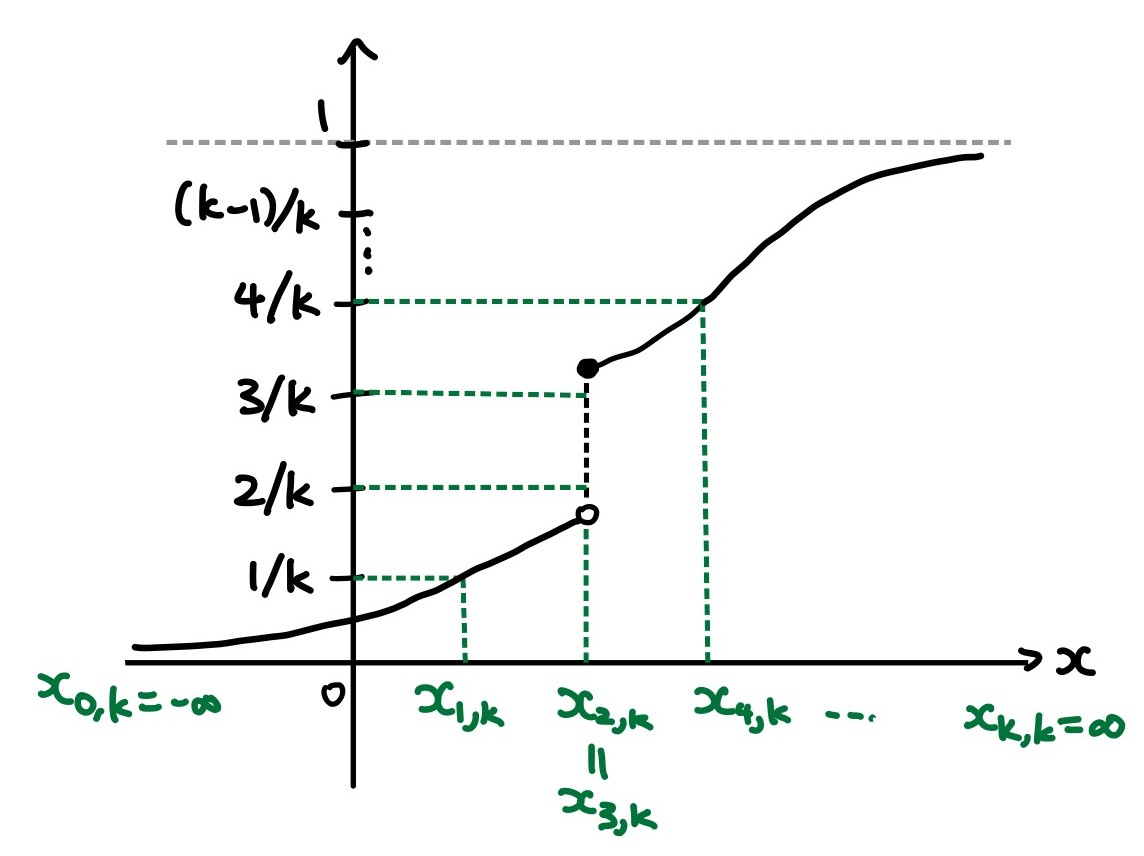
\includegraphics[scale=0.3]{figures/Fig1.2.jpg}
\captionof{figure}{An illustration of knot points}
\end{center}
\vspace{12pt}

By pointwise convergence, for all $j=1,...,k-1$ there are positive integers $N_{j,k,\omega}$ such that for all $n \geq N_{j,k,\omega}$ we have 
\begin{equation*}
|[F_n(\omega)](x_{j,k}) - F_\xi(x_{j,k})| < 1/2k.
\end{equation*}

There are also positive integers $N^-_{j,k,\omega}$ such that for all $n \geq N_{j,k,\omega}$ we have 
\begin{equation*}
|[F_n(\omega)](x_{j,k}-) - F_\xi(x_{j,k}-)| < 1/2k.
\end{equation*}

Take $N_{k,\omega} = \max{(\max_{j=1,...,k-1} N_{j,k,\omega}, \max_{j=1,...,k-1} N^-_{j,k,\omega})}$, we have for all $n \geq N_{k,\omega}$,
\begin{equation*}
\forall j = 1,...,k-1, \quad |[F_n(\omega)](x_{j,k}) - F_\xi(x_{j,k})| < 1/2k.
\end{equation*}
Now let $x \in \R$ be falling into one of the intervals $[x_{j,k}, x_{j+1,k})$. We immediately have
\begin{equation*}
    [F_n(\omega)](x_{j,k}) \leq [F_n(\omega)](x) \leq [F_n(\omega)](x_{j,k+1}-) \leq [F_n(\omega)](x_{j,k+1}).
\end{equation*}
In particular, when $n \geq N_{k,\omega}$, we have
\begin{gather*}
    F_\xi(x_{j,k})-1/2k < [F_n((\omega)](x_{j,k}) F_\xi(x_{j,k})+1/2k, \\
    F_\xi(x_{j+1,k}-)-1/2k \leq [F_n(\omega)](x_{j+1,k}-) < F_\xi(x_{j+1,k}-)+1/2k.
\end{gather*}
This lead to 
\begin{equation*}
[F_n(\omega)](x) \in \bracket{F_\xi(x_{j,k})-\frac{1}{2k}, \,  F_\xi(x_{j+1,k})+\frac{1}{2k}}
\end{equation*}
\newpage

But we also have 
\begin{equation*}
F_\xi(x) \in \left[ F_\xi(x_{j,k}), \,  F_\xi(x_{j+1,k}-) \right) \subseteq \bracket{F_\xi(x_{j,k})-\frac{1}{2k}, \,  F_\xi(x_{j+1,k})+\frac{1}{2k}}
\end{equation*}

\begin{center}
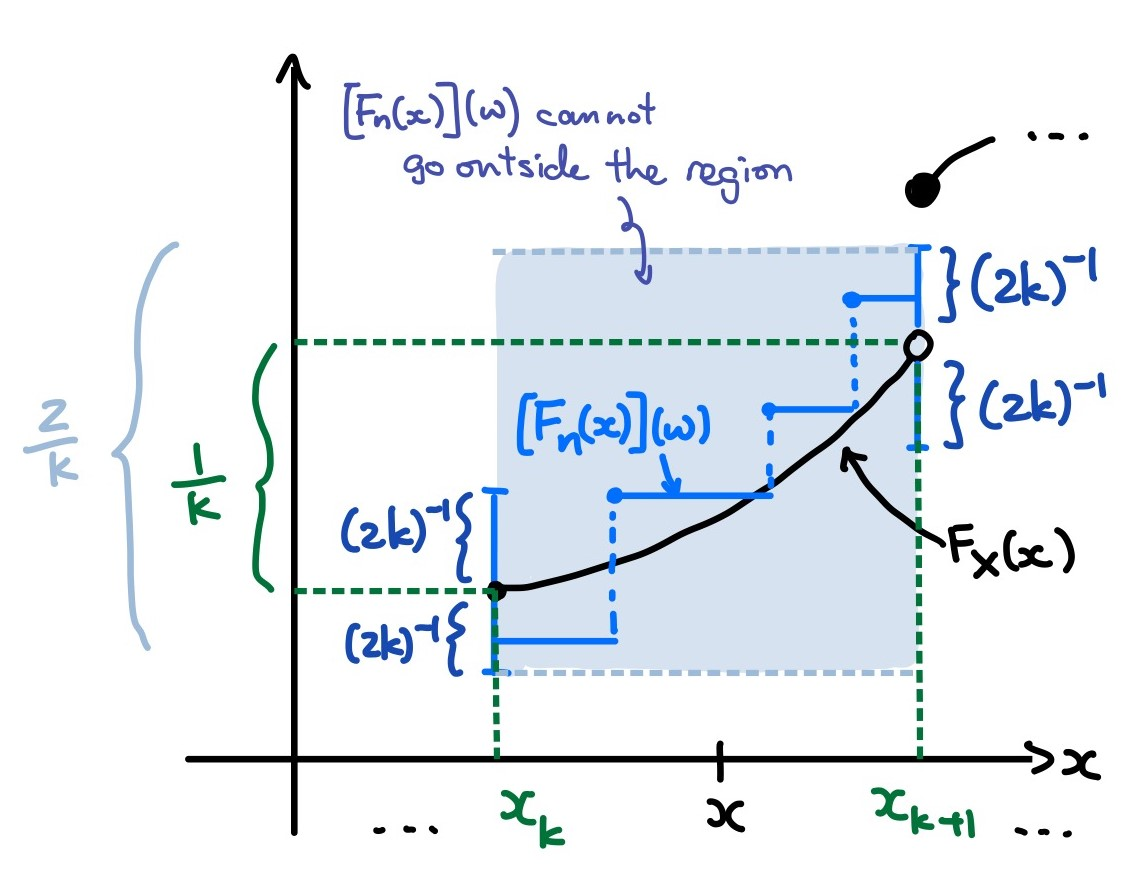
\includegraphics[scale=0.3]{figures/Fig1.3.jpg}
\end{center}
\captionof{figure}{The bound of $[F_n(\omega)](x)$ (labelled as $[F_n(x)](\omega)$) for $x \in [x_{j,k}, x_{j,k+1})$}
\vspace{12pt}
The interval at RHS has length $2/k$, so $|[F_n(\omega)](x) - F_X(x)| < 2/k < \epsilon$. This leads to uniform convergence.
\end{proof}

\begin{remark}
We note that there is an analogue of the central limit theorem, which says that as $n \to \infty$,
\begin{equation}
\sqrt{n} \sup_x \abs{[F_n(x)](\omega) - F_X(x)} \xrightarrow{d} \mathsf{KS} 
\end{equation}
where $\mathsf{KS}$ is the Kolmogorov-Smirnov distribution, defined on $[0,\infty)$ with distribution function
\begin{equation}
F_{\mathsf{KS}}(\alpha) = 1-2 \sum_{n=1}^\infty (-1)^{n+1} e^{-2n^2\alpha^2}.
\end{equation}
If interested, please refer to the 
\end{remark}
\end{unexaminable}

\subsection{Interlude: Stochastic processes*}

\begin{unexaminable}
We will soon move on from the discussion of limiting theorems to stochastic analysis. Stochastic analysis studies the class of objects called stochastic processes, which is now defined below: 
\begin{definition}[Stochastic Process]
Stochastic process $(\xi_\alpha)_{\alpha \in A}$ with index $\alpha$ is a collection of random variables on a common probability space $(\Omega,\F,\p)$.
\end{definition}

For simplicity we assume the output of a stochastic process be a Polish space $(X,\B(X))$ equipped with metric $d$, e.g. $(\R^n, \B(\R^n))$ or $(\C,\B(\C)^n)$. We have already seen two examples of stochastic processes in the previous sections:
\begin{itemize}
\item The \textit{discrete random walk} $(S_n)_{n\geq 1}$, with $S_n := \xi_1 + ... + \xi_n$, where $\xi_1, \xi_2,...$ are defined on a common probability space and being i.i.d. The collection $(S_n)_{n\geq 1}$ is a stochastic process indexed with $n \in \N$.
\item There are some "continuous" analogues of the above random walk, in the sense that it has a "continuous" index $t \in \R$. One of the most important ones is the Brownian motion $W_t$.
\item The empirical distribution function $[F(\omega)](x)$ is also a stochastic process indexed by $x \in \R$.
\end{itemize}

We will focus on the case when the index set $A$ has a metric and total order, e.g. $A = \N, \Z, \Q, \R, [0,\infty)$, as they represent "time". Nevertheless, we may let $A$ be anything. In fact, we let $A = L^2(\R)$ when studying empirical process theory.\\

An important remark is that one may view stochastic processes as one single random variable with outputs as maps $\alpha \mapsto \xi_\alpha(\omega)$. Often the images of these single random variables are Polish spaces. For instance,
\begin{itemize}
\item The \textit{discrete random walk} $(S_n)_{n\geq 1}$ can be viewed as a single random variable taking values in $(\R^\N, \B(\R^\N))$.
\item The Brownian motion $W_t$ can be viewed as a single random variable taking values in $(C^0[0,\infty), \B(C^0[0,\infty)))$, equipped with the uniform norm.
\item The empirical distribution function $[F(\omega)](x)$ is also a stochastic process taking values in the space of the distribution function. Notice that this is a closed subspace of the Skorohod space $(D(\R), \B(D(\R)))$, equipped with the Skorokhod metric.
\end{itemize}
If you have studied weak convergence of measures in general Polish space (see chapter), then you will have a head-start in studying stochastic analysis, but you can probably still survive if you haven't so.
\end{unexaminable}
\newpage

\part{Foundations of Stochastic Processes}
\section{Conditioning and Disintegration}
In studying stochastic processes $(\xi_\alpha)_{\alpha \in A}$, we want to see how different random variables are related to each other. In particular, we want to see if observing one random variable will give more information on other random variables. For this, we need the notion of conditional probability and expectation.

\subsection{Conditional Probability}
\subsubsection{The Discrete Case}
Let $(\Omega, \F, \p)$ be a probability space. We recall the notions of conditional probability on an event: 

\begin{definition}[Conditional Probabilities]
Let $B \in \F$ be an event with $\p(B) > 0$. The \textit{conditional probability of $A$ with respect to $B$} is 
\begin{equation}
    \p(A \,|\, B) = \frac{\p(A \cap B)}{\p(B)}, \quad A\in \F.
\end{equation}
By convention, if $\p(B) = 0$ then we set $\p(A \,|\, B) = 0$
\end{definition}

\begin{exercise}
Check that $\p(\cdot | B)$ is a measure on $\F$.
\end{exercise}

Conditioning should be relative to information one has and $\sigma$-algebra are the natural carriers or descriptions for information content. We would thus like to condition on a $\sigma$-algebra. In the example above, we could replace $B$ by its complement $B^c$ and obtain a new measure $\p(A|B^c)$. Now, for any $\omega \in \Omega$, we have either $\omega \in B$ or $\omega \in B^c$ so it is natural to define
\begin{equation}
    \p(A | \sigma(B))(\omega) := \p(A|B)\chi_B(\omega) + \p(A | B^c)\chi_{B^c}(\omega).
\end{equation}
In this way, for a fixed $\omega \in \Omega$, $\p(\cdot | \sigma(B))(\omega)$ is a probability measure but for a fixed $A\in \F$, $\p(A|\sigma(B))(\cdot)$ is a random variable (taking two values).\\

The sets $B$ and $B^c$ partition $\Omega$, and these ideas carry over to the general partition. 
\begin{definition}[Conditional Expectation on $\sigma$-algebra generated by partition]
    Let $D = \{D_1, D_2, \dots \}$ be a finite or countable partition of $\Omega$ and let $\G = \sigma(D)$. For $A \in \F$ consider the function with values
    \begin{equation} \label{eq:conditional_probability_partition}
        f(\omega) := \p(A | D_i) = \frac{\p(A\cup D_i)}{\p(D_i)}, \quad \text{if }\omega \in D_i.
    \end{equation}
    This function or random variable $f$ is called the \textbf{conditional probability of $A$ given $\G$} and is denoted $\p(A | \G)$. This is written as $\p(A | \G)_\omega$ or $[\p(A | \G)](\omega)$, whenever the argument $\omega$ needs to be explicitly shown.
\end{definition}

\begin{exercise}
Convince yourself that if $\G = \set{\emptyset, \Omega}$ then $f(\omega) := [\p(A\,|\,\G)](\omega)$ is the constant function $f(\omega) := \p(A)$.
\end{exercise}

If the observer learns which element $D_i$ of the partition it is that contains $\omega$, then his new probability for the event $\omega \in A$ is $f(\omega)$. The partition $\{D_i\}$, or equivalently the $\sigma$-algebra, $\G$, can be regarded as an experiment, and to learn which $D_i$ it is that contains $\omega$ is to learn the outcome of the experiment. Thus $\p(A | \G)$ is a function whose value on $D_i$ is the ordinary conditional probability $\p(A | D_i)$. This definition needs to be completed, because $\p(A | D_i)$ is not defined if $\p(D_i) = 0$. In this case $\p(A | \G)$ will be taken to have any constant value on $D_i$; the value is arbitrary but must be the same over all of the set $D_i$.
\begin{example}
Suppose that $X_0, X_1, \dots$ is a Markov chain with state space $S$. The events
\begin{equation*}
    \{ X_0 = i_0,\dots, X_n = i_n \}, \quad i_0,\dots, i_n \in S
\end{equation*}
form a finite or countable partition of $\Omega$. If $\G_n$ is the $\sigma$-algebra generated by this partition, then by the defining condition for Markov chains, 
\begin{equation*}
    \p(X_{n+1} = j | \G_n)_\omega = \p(X_{n+1} = j|X_n = i_n),
\end{equation*}
for $\omega \in \{ X_0 = i_0,\dots, X_n = i_n \}$, $i_0,\dots, i_n \in S$. The sets $\{X_n = i \}$ for $i\in S$ also partition $\Omega$, and they generate a $\sigma$-algebra $\G_n^0$ smaller than $\G_n$. Now 
\begin{equation*}
    \p(X_{n+1} = j | \G_n^0)_\omega = \p(X_{n+1} | X_n = i),
\end{equation*}
for $\omega \in \{X_n = i\}, i \in S$, and the essence of the Markov property is that 
\begin{equation*}
    \p(X_{n+1} | \G_n) = \p(X_{n+1}|\G_n^0).
\end{equation*}
\end{example} 
\subsubsection{The General Case}
If $\G$ is the $\sigma$-algebra generated by a partition $D_1, D_2, \dots$, then the general element of $\G$ is a disjoint union $D_{i_1} \cup \D_{i_2} \cup \cdots$, finite or countable, of certain of the $D_i$. To know which set $D_i$ it is that contains $\omega$ is the same thing as to know which sets in $\G$ contain $\omega$ and which do not. This second way of looking at the matter carries over to the general $\sigma-$algebra $\G$ contained in $\F$ (as always, we have the probability space $(\Omega, \F, \p)$). The $\sigma-$algebra $\G$ will not in general come from a partition as above.\\

One can imagine an observer who knows for each $G$ in $\G$ whether $\omega \in G$ or $\omega \in G^c$. Thus the $\sigma$-algebra $\G$ can in principle be identified with an experiment or observation. Is is natural to try and define conditional probabilities $\p(A | \G)$ with respect to the experiment $\G$. To do this, fix an $\A$ in $\F$ and define a finite measure $\nu$ on $\G$ by
\begin{equation}
    \nu (G) = \p(A \cap G), \quad G \in \G.
\end{equation}
Then $\p(G) = 0$ implies that $\nu (G) = 0$. The Radon-Nikodym theorem can be applied to the measures $\nu$ and $\p$ on the measurable space $(\Omega, \G)$ because the first one is absolutely continuous with respect to the second. It follows that there exists a function or a random variable $f$, which is $\G-$measurable and integrable with respect to $\p$, such that 
\begin{equation}
    \p(A \cap G) = \nu (G) = \int_G f \d \p,
\end{equation}
for all $G$ in $\G$. Denote this function $f$ by $\p(A | \G)$. It is a random variable with two properties:
\begin{enumerate}[(i)]
    \item $\p(A | \G)$ is $\G$-measurable and integrable
    \item $\p(A | \G)$ satisfies the functional equation
    \begin{equation} \label{eq:conditional_probability_sigma_algebra}
        \int_G \p(A | \G) \d \p = \p(A \cap G), \quad G \in \G.
    \end{equation}
\end{enumerate}
There will in general be many such random variables $\p(A | \G)$, but any two of them are equal with probability $1$.\\

If $\G$ is generated by a partition $D_1, D_2, \dots$, the function $f$ defined by $(8.1)$ is $\G$-measurable because $\{ \omega: f(\omega) \in H \}$ is the union of those $D_i$ over which the constant value of $f$ lies in $H$. Any $G$ in $\G$ is a disjoint union $G = \bigcup_{k} D_{i_k}$, and 
\begin{equation}
    \p(A \cap G) = \sum_k \p(A | D_{i_k})\p(D_{i_k}),
\end{equation}
so that \eqref{eq:conditional_probability_partition} satisfies \eqref{eq:conditional_probability_sigma_algebra} as well. Thus the general definition is an extension of the one for the discrete case.\\

Condition $(i)$ above requires that the values of $\p(A|\G)$ depend only on the sets in $\G$. An observer who knows the outcome of $\G$ viewed as an experiment knows for each $G$ in $\G$ whether it contains $\omega$ or not. For each $x$ he knows this in particular for the set $\{\omega' : \p(A|\G)_{\omega'} = x\}$, and hence he knows in principle the functional value $\p(A|\G)_\omega$ even if he does not know $\omega$ itself.\\

Condition $(ii)$ has a gambling interpretation. Suppose that the observer, after he has learned the outcome of $\G$ is offered the opportunity to bet on the event $A$ (unless $A$ lies in $\G$, he does not yet know whether or not it occurred). He is required to pay an entry fee of $\p(A|\G)$ units and will win $1$ unit if $A$ occurs and nothing otherwise. If the observer decides to bet and pays the fee, he gains $1 - \p(A|\G)$ if $A$ occurs and $-\p(A | \G$ otherwise, so that his gain is 
\begin{equation*}
    (1 - \p(A | \G)) \chi_A + (-\p(A|\G))\chi_{A^c} = \chi_A - \p(A | \G).
\end{equation*}
If he declines to bet, his gain is of course $0$. Suppose that he adopts the strategy of betting if $G$ occurs but not otherwise, where $G$ is some set in $\G$. He can actually carry out this strategy, since after learning the outcome of the experiment $\G$ he knows whether or not $G$ occurred. His expected gain with this strategy is his gin integrated over $G$:
\begin{equation*}
    \int_G (\chi_A - \p(A | \G)) \d \p.
\end{equation*}
But \eqref{eq:conditional_probability_sigma_algebra} is exactly the requirement that this vanish for each $G$ in $\G$. Condition $(ii)$ requires then that each strategy be fair in the sense that the observer stands neither to win nor to lose on the average. Thus $\p(A | \G)$ is just entry fee, as intuition requires.\\


\subsection{Conditional Expectation}
We now develop the theory of condition expectation from first principles. 

\begin{definition}[Conditional expectation] \label{def:conditional_expectation}
Suppose that $\xi$ is an integrable random variable on $(\Omega, \F, \p)$ and that $\G$ is a $\sigma-$algebra contained in $\F$. There exists a random variable $\E[\xi | \G]$, called \textbf{conditional expectation of $\xi$ given $\G$}, having these two properties:
\begin{itemize}
    \item $\E[\xi | \G]$ is $\G$-measurable and integrable.
    \item For every $G \in \G$,
    \begin{equation} \label{eq:condtional_expectation}
        \E[\chi_G \E[\xi | \G]] = \int_G \E[\xi | \G] \d \p = \int_G \xi \d \p = \E[\chi_G \xi]
    \end{equation}
\end{itemize}
\end{definition}

\begin{theorem}[Existence of conditional expectation] Whenever $\xi$ is an integrabl random variable on $(\Omega, \F, \p)$, and that $\G$ is a $\sigma$-algebra contained in $\F$, then $\E[\xi \,|\, \G]$ exists, and is unique almost everywhere.
\end{theorem}

To prove the existence of such a random variable, we recall the following generalised version of the Randon-Nikodym theorem.

\begin{theorem}[Radon-Nikodym Theorem]
Let $(\Omega, \F)$ be a measure space, $\mu$ - a finite measure on $\F$. Let $\lambda$ be a measure on $\F$ a.c. with respect to $\mu$ (i.e. $\lambda (A) = 0$ whenever $\mu(A)=0)$. Then there exists an $\F$-measurable function $f$ such that 
\begin{equation}
    \lambda(A) = \int_A f \d \mu \quad \forall A \in \F.
\end{equation}
This function is determined uniquely, up to sets of measure zero. It is called the derivative of $\lambda$ w.r.t. $\mu: f = \frac{\d \lambda}{\d \mu}$. 
\end{theorem}

Consider first the case of nonnegative $\xi$. Define a measure $\nu$ on $\G$ by
\begin{equation*}
    \nu(G) = \int_G \xi \, \d \p.
\end{equation*}
This measure is finite because $\xi$ is integrable, and it is absolutely continuous with respect to $\p$. By the Radon-Nikodym theorem there is a function $f$, $\G-$measurable, such that $\nu(G) = \int_G f \d \p$. This $f$ has the two properties of our definition. If $\xi$ is not necessarily nonnegative, $\E[\xi^+ | \G] - \R[\xi^- | \G]$ clearly has the required properties. \\

There will in general be many such random variables $\E[\xi | \G]$. Any one of them is called a version of the conditional expected value. Any two versions are equal with probability $1$.

\begin{example}[Conditioning on $\sigma$-algbera generated by partition]
Suppose that $G_1, G_2, \dots$ is a finite or countable partition of $\Omega$ generating the $\sigma-$algebra $\G$. Then $\E[\xi | \G]$ must, since it is $\G-$measurable, have some constant value over $G_i$, say $\alpha_i$. Then
\begin{align}
    \int_{G_i} \E[\xi | \G] \d \p &= \int_{G_i} \alpha_i \, \d \p = \alpha_i \p(G_i).
\end{align}
Therefore,
\begin{equation}
    \alpha_i \p (G_i) = \int_{G_i} \xi \d \p,
\end{equation}
which implies
\begin{equation}
    \E[\xi | \G]_\omega = \frac{1}{\p(G_i)} \int_{G_i} \xi \d \p, \quad \omega \in \G_i.
\end{equation}
If $\p(G_i) = 0$, then the value of $\E[\xi | \G]$ over $G_i$ is constant but arbitrary.
\end{example}

To familiarise yourself with the definition of conditional expectation on a $\sigma$-algebra, we provide the following exercise.
\begin{exercise} \label{ex:tower_property}
\begin{enumerate}
    \item[]
    \item Convince yourself that if $\G = \set{\emptyset, \Omega}$ then $[\E[\xi\,|\,\G]](\omega)$ is equal to the constant function $f(\omega) := \E(\xi)$ almost everywhere.
    \item More challenging: let's say you know that $\xi$ is independent of $\G$, which means that for all $B \in \G$ we have $\xi$ independent of $\chi_B$, then we still have $\E[\xi\,|\,\G] = \E[\xi]$
    \item Convince yourself that $\E[\xi \,|\, \F] = \xi$ almost everywhere.
    \item Show that $\E[\E[\xi \,|\, \G]] = \E[\xi]$.
\end{enumerate}
\end{exercise}

\begin{hint}
All problems can be solved solely by checking the definition. For example, in question 1 you check that equality \eqref{eq:conditional_probability_sigma_algebra} holds for $G = \phi$ and $G = \Omega$, and in question 4 you directly use the equality \eqref{eq:conditional_probability_sigma_algebra} for appropriate choice of $G \in \G$. You should also try to convince yourself that the above results are intuitive, e.g. in question 3 the conditional expectation is the random variable itself since you know everything about the random variable.
\end{hint}

\begin{solution} (For question 2):
This is perhaps the most tricky question, but again we try to resort to the definition \eqref{eq:conditional_probability_sigma_algebra}. Here we want to show for all $G \in \G$
\begin{equation}
    \E[\xi] \E[\chi_G] \E[\chi_G \E[\xi]] = \E[\chi_G \xi]
\end{equation}
which is true by the independence assumption. This makes sense, because the $\sigma$ algebra does not give additional information about the random variable $\xi$.
\end{solution}

The example below links conditional expectation and conditional probabilities.

\begin{example}[Conditional expectation of indicator function]
For an indicator random variable $\chi_A$ the defining properties of $\E[\chi_A | \G]$ and $\p(A| \G)$ coincide, therefore 
\begin{equation}
    \E[\chi_A | \G] = \p(A | \G)
\end{equation}
almost surely. For a simple random variable $\xi = \sum \alpha_i \chi_{A_i}$,
\begin{equation}
    \E[\xi | \G] = \sum \alpha_i \p(A_i | \G)
\end{equation}
almost surely.
\end{example}

\subsection{Properties of conditional expectation}
We list some of the properties for conditional expectation. Most properties are direct applications of the definition \eqref{eq:conditional_probability_sigma_algebra}, and we encourage you to prove them by yourselves. The proofs are, however, still included if you want extra hint to familiarise yourself with the notion of conditional expectation.

\begin{property}[I. Linearity] 
Let $\xi,\eta$ is a random variable on $(\Omega, \F, \p)$ and let $\G$ be a $\sigma-$algebra contained in $\F$. Then, almost surely,
\begin{equation} \label{eq:linearity_conditional_expectation}
    \E[a\xi + b\eta + c \,|\, \G] = a\E[\xi \,|\, \G] + b \E[\eta \,|\, \G ] + c
\end{equation}
\end{property}

\begin{proof}
For all $G \in \G$, we have
\begin{align*}
    \E[\chi_G \E[a\xi + b\eta + c \,|\, \G]] 
    &= \E[\chi_G (a\xi + b\eta + c)] \\
    &= a\E[\chi_G\xi] + b\E[\chi_G \eta] + c\E[\chi_G] \\
    &= a\E[\chi_G \E[\xi\,|\,\G]] + b\E[\chi_G \E[\eta\,|\,\G]] + c\E[\chi_G] \\
    &= \E[\chi_G (a\E[\xi \,|\, \G] + b \E[\eta \,|\, \G ] + c)]
\end{align*}
\end{proof}

\begin{property}[II. Monotonicity] \label{prop:conditional_expectation_monotonicity} 
Let $\xi, \eta$ is a random variable on $(\Omega, \F, \p)$ such that $\xi \leq \eta$ almost surely, and let $\G$ be a $\sigma-$algebra contained in $\F$. Then, almost surely, $\E[\xi\,|\,\G] \leq \E[\eta \,|\, \G]$. The above result also holds when $\geq$ is replaced by $>$.
\end{property}

\begin{proof}
Consider the set $G = \set{\omega\,|\,\E[\xi\,|\,\G] > \E[\eta\,|\,\G]}$. If $\p(G) > 0$ then $\E[\chi_G (\E[\xi\,|\,\G] - \E[\eta\,|\,\G])] > 0$ by our definition of $G$. But we also know that $\E[\chi_G (\E[\xi\,|\,\G] - \E[\eta\,|\,\G])] = \E[\chi_G (\xi-\eta)] \leq 0$, which is a contradiction. So $\p(G) = 0$, and $\E[\chi_G (\E[\xi\,|\,\G] - \E[\eta\,|\,\G])] = 0$. So $\E[(\E[\xi\,|\,\G] - \E[\eta\,|\,\G])] = \E[\chi_{G^C} (\E[\xi\,|\,\G] - \E[\eta\,|\,\G])] \leq 0$, and hence $\E[\xi\,|\,\G] \leq \E[\eta\,|\,\G]$ almost surely.
\end{proof}

Substituting $\xi = 0$, then we know that $\eta \geq 0$ a.s. $\implies$ $\E[\eta\,|\,\G] \geq$ a.s.

\begin{exercise}
Prove that for all integrable $\xi$, we have $|\E[\xi|\G]| \leq \E[|\xi| \, | \G]$.
\end{exercise}

\begin{hint}
Note that $\xi = \xi^+ - \xi^-$ and utilise triangle inequality. Also note that $|\xi| = \xi^+ + \xi^-$.
\end{hint}

We can hence prove a conditional version of Jensen inequality:
\begin{theorem}[Conditional Jensen's Inequality]
Suppose that $(\Omega, \F,\p)$ is a probability space and $\xi$ is an integrable random variable taking values in an open interval $I \subset \R$. Let $g: I \to \R$ be convex and let $\G$ be a sub $\sigma-$algebra of $\F$. If $\E[|g(\xi)|] < \infty$, then
\begin{equation} \label{eq:conditional_Jensen_ineq}
    \E[\varphi(\xi) | \G] \ge \varphi(\E[\xi | \G])  \text{ almost surely.}
\end{equation}
\end{theorem}

\begin{property}[III. Tower/Telescopic Properties] \label{prop:tower_property_general}
Let $(\Omega, \F,\p)$ be a probability space, $\xi$ an integrable random variable and $\F_1, \F_2$ be $\sigma-$algebras with $\F_1 \subseteq \F_2 \subseteq \F$. Then almost surely
\begin{equation}
\E[\E[\xi | \F_2] | \F_1] = \E[\xi | \F_1] = \E[\E[\xi | \F_1] | \F_2]
\end{equation}
\end{property}

\begin{hint}
This is a generalisation of exercise \ref{ex:tower_property}.
\end{hint}

\begin{proof}
The first equality can be proven by just using the definition: consider arbitrary $G \in \F_1$, then $G \in \F_2$ and hence 
\begin{equation}
    \E[\chi_G \E[\xi | \F_2]] = \E[\chi_G \xi] = \E[\chi_G \E[\xi | \F_1]]
\end{equation}
which establish the first equality. The second equality can be proven by using similar method in  question 3 from exercise \ref{ex:tower_property}, noting $\E[\xi\,|\,\F_1]$ is $\F_1$ measurable then it is also $\F_2$ measurable.
\end{proof}

\begin{property}[IV. On Taking Limits Under the Conditional Expectation Sign]
Let $\{ \xi_n \}_{n \ge 1}$ be a sequence of extended random variables.
\begin{enumerate}
    \item (Dominated convergence) If $|\xi_n| \le \eta$, $\E[\eta]<\infty$, and $\xi_n \to \xi$ $(a.s.)$, then
    \begin{equation*}
        \E[\xi_n \,|\, \G] \xrightarrow{a.s.} \E[\xi \,|\, \G]
    \end{equation*}
    and 
    \begin{equation*}
        \E[|\xi_n - \xi| | \G] \xrightarrow{a.s.} 0.
    \end{equation*}
    \item (Monotone convergence) If $\xi_n \ge \eta$, $\E[\eta] > -\infty$, $\xi_n \uparrow \xi \, (a.s.)$ and $\E[|\xi|] < \infty$, then
    \begin{equation*}
        \E[\xi_n | \G] \uparrow \E[\xi | \G] \quad (a.s.)
    \end{equation*}
    \item If $\xi_n \le \eta$, $\E[\eta] < \infty$, and $\xi_n \downarrow \xi \, (a.s.)$, then
    \begin{equation*}
        \E[\xi_n | \G] \downarrow \E[\xi | \G] \quad (a.s.)
    \end{equation*}
    \item (Fatou) If $\xi_n \ge \eta $, $\E[\eta] > - \infty$, then
    \begin{equation*}
        \E[\liminf \xi_n | \G] \le \liminf \E[\xi_n | \G] \quad (a.s.)
    \end{equation*}
    \item If $\xi_n \le \eta $, $\E[\eta] < \infty$, then
    \begin{equation*}
        \E[\limsup \xi_n | \G] \le \limsup \E[\xi_n | \G] \quad (a.s.)
    \end{equation*}
    \item (Summation) If $\xi_n \ge 0$ then
    \begin{equation*}
        \E\big[\sum \xi_n | \G \big] = \sum \E[\xi_n | \G] \quad (a.s.)
    \end{equation*}
\end{enumerate}
\end{property}

\begin{proof}
\begin{enumerate}
\item[]
\item Let $\zeta_n = \sup_{m\geq n} |\xi_m - \xi|$. Then $0 \leq |\zeta_n| \leq 2\eta$ and $\zeta_n \to 0$ almost surely, so by DCT we have $\E[\zeta_n] \overset{n\to\infty}\to 0$ Now by triangle inequality, one has 
\begin{equation*}
0 \leq \abs{\E[X_n|\G] - \E[X|\G]} \leq \E[|X_n-X| \,|\, \G] \leq \E[\zeta_n|\G].
\end{equation*}
Since the sequence $\E[\zeta_n|\G](\omega)$ is decreasing on $n$ for fixed $\omega$, the sequence $\E[\zeta_n|\G](\omega)$ exhibits limits $\omega$-almost surely. To evaluate the limit, notice that
\begin{equation*}
0 \leq \E\sqbracket{\lim_{n\to\infty} \E[\zeta_n|\G]} \leq \E\sqbracket{\E[\zeta_n|\G]} = \E[\zeta_n] \overset{n\to\infty}\to 0,
\end{equation*}
so $\lim_{n\to\infty} \E[\zeta_n|\G] = 0$ almost surely, completing the proof.
\item We note from the proof of MCT that one can set $\eta = 0$. Let $\tilde{\xi}_n = \E[\xi_n|\G]$. Then by property II (monotonicity) we have $\tilde{\xi}_n \geq 0$ almost surely and the events $A_n = \set{\tilde{\xi}_n < \tilde{\xi}_{n-1}} \in \G$ has $\p(A_n) = 0$. Let $\tilde{\xi} := \limsup_{n\to\infty} \tilde{\xi}_n$ and $A = \cup_{n\geq 2}$. Then $A \in \G$, $\p(A) = 0$ and for all $\omega \in A^c$ we know that $\tilde{\xi}_n(\omega) \nearrow \tilde{\xi}(\omega)$. We evaluate the limits by noting that for all $G \in \G$,
\begin{equation*}
    \E\sqbracket{\tilde{\xi} \chi_G} = \E\sqbracket{\tilde{\xi}\chi_{G \cap A^c}} \overset{\text{MCT}}= \lim_{n\to\infty} \E\sqbracket{\tilde{\xi}_n \chi_{G \cap A^c}} = \lim_{n\to\infty} \E\sqbracket{\xi \chi_{G \cap A^c}} \overset{\text{MCT}} = \E\sqbracket{\xi\chi_{G \cap A^c}} = \E\sqbracket{\xi\chi_{G}},
\end{equation*}
so we see that $\tilde{\xi}$ is integrable (by taking $G \in \G$) and that $\xi = \tilde{\xi}$ almost surely as desired.
\item This is trivially equivalent to (2) by considering the sequence $\xi - \xi_n$.
\item This is a direct application to (2) by considering the sequence $\eta_n = \inf_{k\geq n} \xi_n$, which is increasing.
\item This is trivially equivalent to (4).
\item This is a direct application to (2).
\end{enumerate}
\end{proof}

\begin{corollary}[V. Factorisation] \label{cor:conditional_expectation_factorisation}
Let $\xi$ and $\eta$ be random variables on $(\Omega, \F, \p)$ with $\xi$, $\eta$ and $\xi \eta $ integrable. Let $\G \subset \F$ be  a $\sigma$-algebra and suppose that $\eta$ is $\G-$measurable. Then
\begin{equation}
	\E[\xi \eta | \G] = \eta \E[\xi | \G] \text{ almost everywhere}
\end{equation}
\end{corollary}

\begin{hint}
Sorry this is not an easy proof. We utilise the four step proof, see chapter 1.
\end{hint}

We finally have the following
\begin{proposition}[$L^2$ orthogonal projection] \label{prop:conditional_expectation_proj}
Suppose $\xi$ is a random variable on $(\Omega,\F,\p)$ such that $\E[\xi^2] < \infty$ (i.e. $\xi \in L^2$). Then $\E[X\,|\,\G]$ is the $L^2$ orthogonal projection onto the subspace 
\begin{equation}
\mathcal{P} = \set{g \in L^2 \,|\, g \text{ is }\G\text{ measurable.}}
\end{equation}
In other words, $\E[X\,|\,\G]$ is the unique minimiser of $\E[X-Y]^2$ for $Y \in \G$.
\end{proposition}

\begin{proof}
We first note that $\E[\E[X\,|\,\G]^2] \leq \E[X^2]$ by conditional Jensen inequality \eqref{eq:conditional_Jensen_ineq}, and that $\E[X\,|\,\G]$ is $\G$-measurable, so $\E[X\,|\,\G] \in \G$. Let $Z$ be a $\G$-measurable function, then \begin{align*}
    \E[X-Z]^2 &= \E[X-\E[X\,|\,\G]+\E[X\,|\,\G]-Z]^2 \\
    &= \E[X-\E[X\,|\,\G]^2 + \E[X\,|\,\G]-Z]^2 + 2\E[(X-\E[X\,|\,\G])(\E[X\,|\,\G]-Z)]
\end{align*}
It remains to show that the cross term is zero. Notice that $\E[X\,|\,\G]-Z$ is $\G$-measurable, so by tower property (exercise \ref{ex:tower_property})
\begin{align*}
    \E[(X-\E[X\,|\,\G])(\E[X\,|\,\G]-Z)] &= \E[\E[(X-\E[X\,|\,\G])(\E[X\,|\,\G]-Z)\,|\, \G]] \\
    &= \E[(\E[X\,|\,\G]-\E[X\,|\,\G])(\E[X\,|\,\G]-Z)] = 0
\end{align*}
the last equality is justified by the factorisation property (corollary \ref{cor:conditional_expectation_factorisation}), linearity and another application of tower property. So we have
\begin{equation}
    \E[X-Z]^2 \geq \E[X-\E[X\,|\,\G]^2 + \E[X\,|\,\G]-Z]^2 \geq \E[X-\E[X\,|\,\G]^2
\end{equation}
with equality holds if $\E[X\,|\,\G]=Z$ almost everywhere.
\end{proof}

\subsection{Conditioning on a random variable}
We define the following
\begin{definition}
The \textit{conditional expectation} of a random variable $\xi$ with respect to a random variable $\eta$ is defined as follows
\begin{equation*}
    \E[\xi | \eta] \equiv \E[\xi | \sigma(\eta)],
\end{equation*}
where $\sigma(\eta)$ is the $\sigma-$algebra generated by $\eta$.
\end{definition}

\begin{theorem}[Representation of conditional expectation] \label{thm:rep_of_conditional_expectation}
There exists a unique (almost everywhere) Borel function $g: \R \to \R$ such that
\begin{equation}
    \E[\xi | \eta] = g(\eta).
\end{equation}
\end{theorem}

The proof is a direct application of the following lemma from measure theory

\begin{lemma}
Let $\mu, \eta$ be random variables on $(\Omega,\F,\p)$. Then $\mu$ be $\sigma(\eta)$-measurable $\iff$ there exists a Borel-measurable function $f: \R \to \R$ such that $\mu = f(\eta)$. 
\end{lemma}

\begin{hint}
We apply four-step proof on $\mu$.
\end{hint}

\begin{proof}
\begin{enumerate}
    \item[]
    \item Let $\mu = \chi_A$ for some $A \in \F$. For $\mu$ to be $\sigma(\eta)$ measurable we must have $A \in \sigma(\eta)$. (Why?) This means there exists $B \in \B(\R)$ such that $\eta^{-1}(B) = A$. We immediate see that $\mu = \chi_B(\eta)$.
    \item Let $\mu$ be a simple random variable such that $\mu = \sum_{i=1}^n c_j \chi_{A_j}$, with $\set{A_j}_{j=1}^n$ partitions $\Omega$. Again we must have $A_j \in \sigma(\eta)$, so for all $j$ there exists $B \in \B(\R)$ such that $\eta^{-1}(B_j) = A_j$. Then $\set{B_j}_{j=1}^n$ partitions $\eta(\Omega)$, and that $\mu = f(\eta)$ with $f = \sum_{i=1}^n c_j \chi_{B_j}(x)$.
    \item We assume $\mu$ being non-negative, then $\mu$ can be approximated by a pointwise non-decreasing sequence of simple random variable which converges pointwise to $\mu$: $\mu_n \nearrow \mu$. Each $\mu_n$ can be represented in the form of $f_n(\eta)$. Choose $f = \sup_{n\geq 1} f_n$, which is Borel measurable, and for all $\omega$, 
    \begin{equation}
        f(\eta(\omega)) = \sup_{n\geq 1} \mu_n(\omega) = \mu(\omega)
    \end{equation}
    \item For general $\mu$, we decompose it into $\mu^+ - \mu^-$, and write $\mu^+ = f^+(\eta)$ and $\mu^- = f^-(\eta)$ by step 3. We let $f = f^+ - f^-$ to complete the proof.
\end{enumerate}
\end{proof}

\begin{example}[Conditional expectation of random variables with joint density] \label{eg:conditional_expectation_joint_rv}
Consider real valued random variables $X,Y$ on same probability space $(\Omega,\F,\p)$. Assume the random vector $(X,Y)$ has continuous joint density $f_{X,Y}(x,y) > 0$. Recall that $X$ has density $f_X(x) = \int_\Omega f_{X,Y}(x,y) \, dy$ and $Y$ has density $f_Y(y) = \int_\Omega f_{X,Y}(x,y) \, dx$. Assume $f_X(x), f_Y(y) > 0$ almost everywhere in $\R$. We want to compute $\E[h(X)\,|\,Y]$ for all Borel-measurable function $h$ with $\E[|h(X)|] < \infty$. By theorem \ref{thm:rep_of_conditional_expectation}, we know that $\E[h(X)\,|\,Y] = \phi(Y)$ for a unique (almost everywhere) Borel-measurable $\phi$. We claim that
\begin{equation} \label{eq:conditional_expectation_rv}
    \phi: y \mapsto \int_\R h(x) \frac{f_{X,Y}(x,y)}{f_Y(y)} \, dx
\end{equation}
We can show this by utilising the definition of conditional expectation: for all $A \in \sigma(Y)$ we have
\begin{equation}
    \E[\chi_A \phi(Y)] = \E[\chi_A h(X)]
\end{equation}
Since $A \in \sigma(Y) \subseteq \F$, we know that $A = Y^{-1}(B)$ for some $B \in \B(\R)$.

\begin{align*}
    \E[\chi_A h(X)] &= \E[\chi_B(Y) h(X)] \\
    &= \int_\R \int_\R h(x) \chi_B(y) f_{X,Y}(x,y) \, dy \, dx \\
    &= \int_\R \int_\R h(x) \chi_B(y) \frac{f_{X,Y}(x,y)}{f_Y(y)} f_Y(y) \, dy \, dx \\
    &\overset{\text{(Tonelli)}}{=} \int_\R \int_\R h(x) \chi_B(y) \frac{f_{X,Y}(x,y)}{f_Y(y)} f_Y(y) \, dx \, dy \\
    &= \int_\R \chi_B(y) \bracket{\int_\R h(x) \frac{f_{X,Y}(x,y)}{f_Y(y)} \, dx} \, f_Y(y) dy \\
    &= \E[\chi_B(Y) \phi(Y)] \\
    &= \E[\chi_A \phi(Y)]
\end{align*}
which completes the proof. In particular, this shows us that if $C = X^{-1}(D)$
\begin{equation} \label{eq:regular_conditional_distribution_joint_rv}
    \p(X \in C \,|\, Y) = Q(Y;C), \; \text{with} \; Q(y;C) = \int_\R \chi_C(x) \frac{f_{X,Y}(x,y)}{f_Y(y)} \, dx
\end{equation}
This example can be generalised to the case when $X,Y$ are random vectors.
\end{example}

\begin{exercise}[Conditional expectation of discrete random variables] \label{ex:conditional_expectation_discrete_rv}
\begin{itemize}
    \item[]
    \item Consider random variables $X,Y$ taking value in $\N$, and assume they have joint mass $p_{X,Y}(x,y)$ for $x,y \in \N$. Assume $h:\N \to \R$ such that $\E[|h(X)|] < \infty$. Using \eqref{eq:conditional_probability_partition}, verify that $\E[h(X)\,|\,Y] = \phi(Y)$, where for $y$ such that $p_Y(y) \neq 0$,
    \begin{equation}
        \phi(y) = \sum_{x\in\N} h(x) \frac{p_X(x,y)}{p_Y(y)}
    \end{equation}
    Notice how this formula is similar to \eqref{eq:conditional_expectation_rv}. What value should we assign to $\phi(y)$ for $p_Y(y) = 0$ if we were to follow our convention about conditional probability on zero-probability events?
    \item Here is an application to the above formula. Consider random variables $Z_1, Z_2$ on $(\Omega,\F,\p)$ with $Z_1 \sim \Po(\lambda_1)$ and $Z_2 \sim \Po(\lambda_2)$. Assume $p = \lambda_1/(\lambda_1+\lambda_2)$, show that
    \begin{equation}
        \p[Z_1 = k \,|\, Z_1 + Z_2 = n] = {n \choose k} p^k (1-p)^{n-k}
    \end{equation}
\end{itemize}
\end{exercise}

We will study the above examples further in the next section. Before that, let us highlight the projection property of conditional expectation.

\begin{proposition}[$L^2$ orthogonal projection II]
If $\E[\xi^2] < \infty$, then 
\begin{equation*}
    \min_f \E[(\xi - f(\eta)^2] = \E[(\xi - \E[\xi | \eta])^2],
\end{equation*}
where min is over all $\sigma(\eta)$-measurable functions such that $\E[f^2(\eta)] < \infty$.
\end{proposition}

\begin{proof}
This is a direct application of proposition \ref{prop:conditional_expectation_proj}.
\end{proof}

We can therefore obtain conditional expectation by obtaining the minimiser of $L^2$ error.

\begin{exercise}[Conditional expectation of normal distribution] Consider random variables $X,Y$ such that they are jointly normally distributed:
\begin{equation}
    \begin{pmatrix} X \\ Y\end{pmatrix} \sim \mathbf{N}_{2} \bracket{ \begin{pmatrix} \mu_X \\ \mu_Y \end{pmatrix}, \begin{pmatrix} \sigma_X^2 & \rho \sigma_X \sigma_Y \\ \rho \sigma_X \sigma_Y & \sigma_Y^2 \end{pmatrix}},
\end{equation}

then $\E[Y|X] = f(X)$. Assume we know that $f(x) = ax+b$, then we know that $a,b$ are minimiser of $\E[Y - aX - b]^2$. Verify that
\begin{equation}
    \E(Y\,|\,X) = \mu_Y + \rho \frac{\sigma_Y}{\sigma_X}(X - \mu_X) = \bracket{\mu_Y - \rho \frac{\sigma_Y}{\sigma_X}\mu_X} + \rho \frac{\sigma_Y}{\sigma_X} X.
\end{equation}
\end{exercise}
\newpage

\subsection{Regular conditional distribution*}
\begin{unexaminable}
Let us revisit the above examples. We know from example \ref{eg:conditional_expectation_joint_rv} that if $(X,Y)$ has joint density $f_{X,Y}(x,y) > 0$ then we have
\begin{equation}
    \p(X \in C \,|\, Y) = Q(Y;C), \; \text{with} \; Q(y;C) = \int_\R \chi_C(x) \frac{f_{X,Y}(x,y)}{f_Y(y)} \, dx.
\end{equation}

There are two ways to interpret $Q(y;C)$. If we fix a set $C \in \F$, then the function $Q(.;C)$ is a $\sigma(Y)$-measurable. On the other hand, if we fix $y \in Y(\Omega)$, then the set function $Q(y;.)$ is a measure on $(\R,\B(\R))$. To see this it is trivial to see that $Q(y;\varnothing) = 0$ and 
\begin{equation}
    Q(y,\R) = \frac{1}{f_Y(y)} \int_\R f_{X,Y}(x,y) \, dx = 1 
\end{equation}

We only need to prove $\sigma$-additivity. Let $A_1, A_2, ...$ be disjoint sets in $\B(\R)$, and let $A = \sqcup_{i\geq 1} A_i$, then by monotone convergence theorem
\begin{align*}
    Q(y,A) = \int_\R \chi_A(x) \frac{f_{X,Y}(x,y)}{f_Y(y)} \, dx 
    &= \int_\R \sum_{i\geq 1} \chi_{A_i}(x) \frac{f_{X,Y}(x,y)}{f_Y(y)} \, dx \\ &\overset{\text{(MCT)}}{=} \sum_{i\geq1} \int_\R \chi_{A_i}(x) \frac{f_{X,Y}(x,y)}{f_Y(y)} \, dx = \sum_{i\geq 1} Q(y,A_i)
\end{align*}

$Q(y,C)$ is hence considered as a \textit{(Markov) stochastic kernel}. In this chapter, we would like to prove that we can construct such transitional kernel $Q_{Y,\G}(\omega, C) = [\p(Y \in C \,|\, \G)](\omega)$ for any random variables $Y$ and $\sigma$-algebra $\G$. We begin by formally defining the notion of transitional kernel

\begin{definition}[Transitional, Stochastic kernel]
Let $(\Omega_1, \F_1)$, $(\Omega_2,\F_2)$ be measurable spaces. A map $Q:\Omega_1 \times \F_2 \to [0,\infty]$ is a \textit{transitional kernel} if
\begin{itemize}
    \item when $A_2 \in \F_2$ is fixed, $Q(.,A_2)$ is a $\F_1$-measurable function.
    \item when $\omega_1 \in \Omega_1$ is fixed, the set function $Q(\omega_1,.)$ is a measure on $(\Omega_2, \F_2)$
\end{itemize}
In addition if $\forall \omega_1 \in \Omega_1$, $Q(\omega_1, \Omega_2) = 1$ (i.e. $Q(\omega_1,.)$ is a probability measure), then $Q$ is a \textit{(Markov) stochastic kernel}. If we have $\forall \omega_1 \in \Omega_1$, $Q(\omega_1, \Omega_2) \leq 1$, then $Q$ is \textit{substochastic}.
\end{definition}

\begin{remark}
A time-homogeneous Markov chain is characterise by a family of stochastic kernels, which explains why stochastic kernels are named after Markov.
\end{remark}

From this, we can define the notion of regular conditional distribution. Here we assume $\xi$ takes value on a general measurable space $(E,\mathcal{E})$.

\begin{definition}[Regular conditional distribution]
Let $\xi:(\Omega,\F) \to (E,\mathcal{E})$ be a random variable, and let $\G$ be a $\sigma$-algebra of $\Omega$ contained in $\F$. A regular conditional distribution of $\xi$ \textbf{given the $\sigma$-algebra} $\G$ is a stochastic kernel $Q: \Omega \times \mathcal{E} \to [0,\infty]$ such that for almost all $\omega \in \Omega$, we have 
\begin{equation} \label{eq:rcd}
    \forall B \in \mathcal{E}, \quad Q(\omega, B) = [\p(\xi \in B \,|\, \G)](\omega)
\end{equation}
In addition, assume $\eta: (\Omega, \sigma(\eta)) \to (E',\mathcal{E}')$ is a random variable (not necessary equal to $(E,\mathcal{E})$), then the conditional distribution of $\xi$ given the \textbf{random variable $\eta$} is the conditional distribution of $\xi$ given on the $\sigma$-algebra $\sigma(\eta)$.
\end{definition}

\begin{remark} \label{rmk:rcd}
Let $Q:\Omega \times \E$ be a regular conditional distribution of $\xi$ given $\eta$, then for almost all $\omega \in \Omega$, and for all $B \in \mathcal{E}$, we have
\begin{equation}
    Q(\omega,B) = [\p(\xi \in B \,|\, \eta)](\omega)
\end{equation}
When $Q$ is restricted so that the above equality is satisfied, then $Q(.,B)$ is $\eta$ measurable, and hence $Q(\omega,B) = \tilde{Q}(\eta(\omega), B)$ for a unique function $\tilde{Q}: (E',\mathcal{E}') \times \mathcal{E} \to [0,\infty]$, such that $\tilde{Q}(.,B)$ is $\mathcal{E}$ measurable for all $B \in \mathcal{E}$. We will also refer to this function $\tilde{Q}$ when talking about regular conditional distribution of $\xi$ on $\eta$.
\end{remark}

\begin{example}[Continuation of Example \ref{eg:conditional_expectation_joint_rv}] Under same settings, we see that $Q(y,C)$ is a regular conditional distribution of $X$ given $Y$ in the sense as described in remark \ref{rmk:rcd}. Note that when $y$ is fixed, then the measure $Q(y,.)$ is absolutely continuous with density $f_{X|Y}(x|y) := f_{X,Y}(x,y)/f_Y(y)$. The function $f_{X|Y}(x|y)$ is known as the \textit{conditional density} of $X$ given $Y$.
\end{example}

\subsubsection{Existence of regular conditional distribution}

We first assume $(E,\mathcal{E})$ to be $(\R,\B(\R))$ for simplicity. The main difficulty of constructing appropriate regular conditional distribution is that the conditional expectation $[\p(Y \in B \,|\, \G)](\omega)$ is unique up to measure-zero set. Moreover, many properties of probability measures only hold almost surely, e.g. monotonicity and continuity from above/below. Fortunately, we only need the equality \eqref{eq:rcd} to hold for almost all $\omega$. Our plan is therefore to construct the stochastic kernel $Q(\omega,B)$ for almost all "good" $\omega$ when all desired properties hold, and extend this kernel to other "bad" $\omega$. This will work if the set of "bad" $\omega$ is measure zero.

\begin{theorem}[Existence of regular conditional distribution for real-valued random variables] \label{thm:existence_rcd}
Let $\xi:(\Omega,\F,\p) \to (\R,\B(\R))$ be a random variable, then for all $\sigma$-algebra $\G \subseteq \F$ we can construct a regular conditional distribution $\xi$ given $\G$.
\end{theorem}

\begin{hint}
We only need to look at $Q(\omega,B)$ for all $B = (-\infty,r]$ for some $r$, since the half intervals $(-\infty,r]$ generates $\B(\R)$. From chapter 1, we list out the desired property for a version of $F(\omega,r) = [\p[\xi \in (-\infty,r] \,|\, \G]](\omega)$ to be a valid distribution function
\begin{enumerate}
    \item $F(\omega,r) \overset{r \to -\infty}{\to} 0$ and $F(\omega,r) \overset{r \to \infty}{\to} 1$
    \item (Monotonicity) $F(\omega,r) \leq F(\omega,s)$ whenever $r \leq s$, and
    \item (Right continuity) $F(\omega, (-\infty,r_n)) \searrow F(\omega,r)$ whenever $r_n \searrow r$.
\end{enumerate}
So there are four cases for $F(\omega, r)$ not to be a distribution function:
\begin{itemize}
    \item $\omega \in A_{r,s} := \set{\omega \,|\, F(\omega,r) > F(\omega,s)}$ for $r \leq s$.
    \item $\omega \in B_r' := \set{\omega \,|\, \text{there exists a sequence } (r_n) \searrow r \text{ such that } F(\omega,r_n) \not\rightarrow F(\omega,r)}$
    \item $\omega \in C' := \set{\omega \,|\, F(\omega,r) \overset{r\to \infty}{\not\rightarrow} 1}$
    \item $\omega \in D' := \set{\omega \,|\, F(\omega,r) \overset{r\to -\infty}{\not\rightarrow} 0}$
\end{itemize}
If we can show that the "bad" set of $\omega$, $G' = (\cup_{r\leq s} \, A_{r,s}) \cup (\cup_r \, B_r) \cup C \cup D$, has measure zero, then we can define $F(\omega,.)$ as followed:
\begin{equation}
    F(\omega, r) = \begin{cases}
    [\p(\xi \in (-\infty, r] \,|\, \G)](\omega) & \omega \in \Omega \setminus G' \\
    F_0(r) & \omega \in F
    \end{cases}
\end{equation}
where $F_0$ can be any appropriate distribution function. Then for all $\omega$, $F(\omega,r)$ is a distribution function, and for almost all $\omega$, $F(\omega,r) = \p(\xi \in (-\infty,r] \,|\, \G)$. \\

We note from property \ref{prop:conditional_expectation_monotonicity} that $A_{r,s}$ has measure zero for any fixed $r,s$, but this does not imply that $\cup_{r\leq s} A_{r,s}$ has measure zero if we only assume $r,s$ are real, since this is an uncountable union. Moreover, even though we know that for a fixed sequence $(r_n) \searrow r$, we have $F(\omega,r_n) \searrow F(\omega,r)$ almost surely in $\omega$, we don't know whether $B_r$ itself has measure zero, since
\begin{equation}
    B_r' = \bigcup_{(r_n) \text{ sequence} \\ (r_n) \searrow r} \set{\omega \,|\, F(\omega,r_n) \not\to F(\omega,r)}
\end{equation}
which is again an uncountable union of measure zero sets. Fortunately, we can refine our analysis by noting the following elementary facts in analysis: (exercise!)
\begin{itemize}
    \item If $f:\R \to \R$ is a monotonic increasing function, then $f$ is right continuous iff for all $x$, there exists a sequence $(x_n) \searrow x$ such that $f(x_n) \to x$ as $n \to \infty$.
    \item $\Q$ is dense in $\R$. As a result, the half-intervals $(-\infty,a], a\in \Q$ generate $\B(\R)$.
\end{itemize}
As a result, we may refine our analysis by considering $F(\omega,r)$ for all $r \in \Q$, then extend our analysis to $r \in \R$.
\end{hint}

\begin{proof}
We redefine the sets of "bad" $\omega$.
\begin{itemize}
    \item $\omega \in A_{r,s} := \set{\omega \,|\, F(\omega,r) > F(\omega,s)}$ for $r \leq s$
    \item $\omega \in B_r := \set{\omega \,|\, F(\omega, r + 1/n) \not\rightarrow F(\omega,r)}$
    \item $\omega \in C := \set{\omega \,|\, F(\omega,n) \overset{n\to \infty}{\not\rightarrow} 1}, n \in \Z_{\geq 1}$
    \item $\omega \in D := \set{\omega \,|\, F(\omega,-n) \overset{n\to \infty}{\not\rightarrow} 0}, n \in \Z_{\geq 1}$.
\end{itemize}
Define 
\begin{equation}
    G = \bracket{\bigcup_{r\leq s, \\ r,s \in \Q} A_{r,s}} \cup \bracket{\bigcup_{r \in \Q} B_r} \cup C \cup D
\end{equation}
Then $G$ is a countable union of measure-zero sets, and so $G$ is also measure-zero. Hence if we define
\begin{equation}
    F(\omega, z) = \begin{cases}
    \inf\bracket{[\p(\xi \in (-\infty, r] \,|\, \G)](\omega) \,:\, r \in \Q, r > z} & \omega \in \Omega \setminus G \\
    F_0(z) & \omega \in F
    \end{cases}
\end{equation}
then it is a valid distribution function for all $\omega$, and by chapter 1 we can assign a measure $Q(\omega,.)$ to each of the distribution $F(\omega,.)$. Be reminded that $Q(\omega,B)$ is itself a measurable function for all $B \in \B(\R)$, we have therefore constructed a stochastic kernel. \\

We finally check that $Q$ is actually a regular conditional distribution, i.e. for all $A \in \G$,
\begin{equation}
    \E[\chi_A(\omega) Q(\omega, B)] = \E[\chi_{A \cap \set{\xi \in B}}] = \p(A \cap \set{\xi \in B})
\end{equation}
Fix an arbitrary $A \in \G$, then we see that the above equality holds for all $B = (-\infty,r]$ where $r \in \Q$, and hence we can extend the equality to for all $B \in \B(\R)$.
\end{proof}

\begin{remark}
We can extend the above result to any Polish spaces $(E,\mathcal{E})$, for instance $\R^n$ and $C^0([0,1])$ equipped with supremum norm. To do so (theoretically) we note that there is a bijective map $\varphi:(E,\mathcal{E}) \to (\R,\B(\R))$ such that $\varphi$ is $\mathcal{E}$ measurable and $\varphi^{-1}$ is $\B(\R)$ measurable. We can hence construct regular conditional distribution on $\xi:(\Omega,\F) \to (E,\mathcal{E})$ by constructing a regular conditional distribution on $\xi' = \phi \circ \xi: (\Omega,\F) \to (\R,\B(\R))$, denote as $\overline{Q}:\Omega \times \B(\R) \to [0,\infty]$. Then the stochastic kernel $Q(\omega,A) = \overline{Q}(\omega,\phi(A)) : \Omega \times \mathcal{E} \to [0,\infty]$ is indeed a regular conditional distribution of $\xi$.
\end{remark}

\subsubsection{Further Examples}

\begin{example}[Continuation of exercise \ref{ex:conditional_expectation_discrete_rv}]
 Consider random variables $Z_1, Z_2$ on $(\Omega,\F,\p)$ with $Z_1 \sim \Po(\lambda_1)$ and $Z_2 \sim \Po(\lambda_2)$. Assume $p = \lambda_1/(\lambda_1+\lambda_2)$. We have shown that the following regular conditional distribution of $Z_1$ given $Z_1 + Z_2$
\begin{equation}
    \p[Z_1 = k \,|\, Z_1 + Z_2 = n] = {n \choose k} p^k (1-p)^{n-k}
\end{equation}
is actually the probability mass of a binomial distribution $\mathsf{B}(n,p)$. As a result, we may abuse definitions to say that of $Z_1$ given $Z_1 + Z_2$ is "$\mathsf{B}(n,p)$" distributed, written as $Z_1 \,|\, Z_1 + Z_2 \sim \mathsf{B}(n,p)$.
\end{example}

\begin{exercise}[Evaluating conditional expectation from conditional distribution]
Let $Q(\omega,B)$ be a regular conditional distribution of random variable $\xi: (\Omega,\F,\p) \to (E,\mathcal{E})$ given $\sigma$-algebra $\G\subseteq\F$. Assume $h:(E,\mathcal{E}) \to (\R,\B(\R))$ is a $\mathcal{E}$-measurable function such that $\E|h(\xi)| < \infty$. 
\begin{enumerate}
    \item Show that
\begin{equation}
    [\E[h(\xi)\,|\,\G]](\omega) = \int h(x) Q(\omega, dx) 
\end{equation}
where the integral at the RHS is defined so that
\begin{equation}
    \int \chi_B(x) Q(\omega, dx) = \int \chi_B(x) \, dQ(\omega, .) =  Q(\omega,B)
\end{equation}
    \item Define the map $\overline{Q}$ mapping $f$ as a bounded function on $(E,\mathcal{E})$ to a function $\overline{Q}f$ on $(\Omega,\F)$ such that:
    \begin{equation}
        \overline{Q}: f \mapsto \bracket{\omega \mapsto \int f(x) \, Q(\omega, dx)}
    \end{equation}
    Show that $\overline{Q}f$ is bounded, and that $\overline{Q}$ is a contraction int the following sense:
    \begin{equation}
        \sup_{\omega \in \Omega} |\overline{Q}f(\omega)| \leq \sup_{x \in E} |f(x)|
    \end{equation}
\end{enumerate}
\end{exercise}

\begin{hint}
For question 1, one can prove the desired result to $h$ being simple function by using linearity of integrals. Then follow the remaining steps of the four-step proof by utilising appropriate convergence theorems.
\end{hint}

\begin{exercise}[Bayesian Analysis]
\begin{enumerate}
    \item[]
    \item Construct a random vector $(\lambda,N): (\Omega,\F) \to ([0,\infty), \B([0,\infty))) \otimes (\N, 2^\N)$ such that $\lambda \sim \Gamma(\alpha,\beta)$ and $N \,|\, \lambda \sim \Po(\lambda)$.
    \item Show that $\lambda \,|\, N$ follows a Poisson distribution with a suitable parameter as a function of $N$.
\end{enumerate}
\end{exercise}
\end{unexaminable}
\newpage

\vfill
\begin{center}
    \textbf{- End of Probability Theory -}
\end{center}
\newpage

\nopagecolor
\bibliographystyle{vancouver}
\bibliography{export}
\end{document}
